\documentclass[UTF8]{ctexbook}

\usepackage[a4paper,margin=2.5cm]{geometry}\usepackage{amsmath,amssymb,amsthm}
\usepackage{graphicx}
\graphicspath{{image/}}
\usepackage{float}
\usepackage{subcaption}
\usepackage{hyperref}
\usepackage{booktabs}
\usepackage{longtable}
\usepackage{tabularx}
\usepackage{tikz}

\usepackage[version=4]{mhchem}
\usepackage{chemfig}
\setchemfig{bond offset=1pt, atom sep=2.2em, cram width=1.6ex}

\usetikzlibrary{arrows.meta,positioning,calc}
\newcommand{\R}{\mathbb{R}}
\raggedbottom
\hfuzz=30pt
\vfuzz=30pt
\tracinglostchars=0

\begin{document}
\tableofcontents

% ---- chunk ch1_2 : 1.2 化学热力学与动力学 ----

\chapter{化学物理原理}

\section{化学反应热力学}

化学反应能否发生、能放出多少热、最终停在什么位置，是热力学要回答的问题。本节先把能量与方向性拆成焓与熵，再合成为吉布斯自由能；随后给出处理溶液平衡的三件通用工具——分布系数、守恒方程组、活度与条件常数；在此基础上讨论化学平衡的移动与多重平衡；最后把平衡条件用于电子转移，得到电极电势与能斯特方程。

\subsection{焓变}

热力学第一定律给出内能变化的普遍形式。若系统只做体积功，则
\begin{equation}
dU=\delta Q-p\,dV .
\end{equation}
化学反应中我们能够直接测量的是热量，而测量条件通常只有两种极端：恒容与恒压。

恒容条件下，体积功为零，弹式量热计测得的反应热直接等于内能变化：
\begin{equation}
Q_V=\Delta U .
\end{equation}
恒压条件下，杯式量热计测得的热量包含了系统对抗外压所做的体积功：
\begin{equation}
\Delta U=Q_P-p\Delta V,
\qquad\text{即}\qquad
Q_P=\Delta U+p\Delta V .
\end{equation}
由于大多数化学过程在大气中进行，恒压情形更为常见。为把 $Q_P$ 也写成一个状态函数的增量，定义焓
\begin{equation}
H=U+pV,
\end{equation}
于是恒压反应热就是焓变：
\begin{equation}
\Delta H=Q_P=\Delta U+p\Delta V .
\end{equation}
焓是状态函数，其变化只取决于始态与终态，与路径无关。这一点使焓变成为热化学计算的基本量。

对一般反应 $aA+bB\to cC+dD$，引入反应进度
\begin{equation}
\xi=\frac{n_i-n_{i,0}}{\nu_i},
\end{equation}
其中 $\nu_i$ 为化学计量数（反应物取负、产物取正）。反应焓变与反应进度之比即摩尔反应焓变 $\Delta_rH_m=\Delta_rH/\xi$。为了在不同实验之间比较，还要规定标准状态：通常取 $p^\theta=100~\mathrm{kPa}$、$c^\theta=1~\mathrm{mol\cdot L^{-1}}$、$T=298.15~\mathrm{K}$，此时的标准摩尔反应焓变记为 $\Delta_rH_m^\theta$。

若想由各物质的焓直接计算反应焓变，会遇到一个根本困难：焓包含内能，而内能不能被直接测量。因此焓的零点只能人为规定。热化学约定，最稳定单质的标准摩尔生成焓为零：
\begin{equation}
\Delta_fH_m^\theta(\text{最稳定单质})=0 .
\end{equation}
任何化合物的生成焓则定义为由单质生成 $1~\mathrm{mol}$ 该物质时的焓变。于是任意反应的焓变可以写成产物与反应物生成焓的代数和：
\begin{equation}
\Delta_rH_m^\theta=\sum_i\nu_i\,\Delta_fH_m^\theta(\text{生成物})
-\sum_i\nu_i\,\Delta_fH_m^\theta(\text{反应物}).
\end{equation}
这条式子的意义在于，它把一个无法直接测量的绝对量转化成了可以查表求得的标准生成焓，从而使热化学计算成为可能。

\subsection{熵变}

熵描述系统的混乱程度。若已知系统的微观状态数 $\Omega$，玻尔兹曼给出的定义是
\begin{equation}
S=k_{\mathrm B}\ln\Omega ,
\end{equation}
其中 $k_{\mathrm B}$ 为玻尔兹曼常数。微观状态数越多，系统可选择的排布方式越多，熵越大。

化学中更常用的是克劳修斯熵，它来自对热机循环的分析。卡诺循环由两个等温过程和两个绝热过程组成，工作在高温热源 $T_h$ 与低温热源 $T_c$ 之间。若高温热源向工作物质传热 $Q_h>0$，工作物质向低温热源传热 $Q_c<0$，则热机效率为
\begin{equation}
\eta=1-\frac{|Q_c|}{Q_h}=1-\frac{T_c}{T_h}.
\end{equation}
整理得
\begin{equation}
\frac{Q_c}{T_c}+\frac{Q_h}{T_h}=0 .
\end{equation}
也就是说，在一个可逆的卡诺循环中，各段热温商之和为零。

把任意一个可逆循环（在 $p$--$V$ 图上是一条闭合曲线）用许多绝热线和等温线切成无数个微小的卡诺循环：相邻小循环共用的绝热过程一正一反、相互抵消，所有小循环的外轮廓便逼近原来的任意循环。于是对任意可逆循环都有
\begin{equation}
\oint\frac{\delta Q_{\mathrm{rev}}}{T}=0 .
\end{equation}
这说明 $\delta Q_{\mathrm{rev}}/T$ 是某个状态函数的全微分。定义熵
\begin{equation}
dS=\frac{\delta Q_{\mathrm{rev}}}{T},
\end{equation}
它只由始末状态决定，与路径无关。

若循环不可逆，热机效率总是低于卡诺效率，重复上述论证便得到克劳修斯不等式
\begin{equation}
dS\geq\frac{\delta Q}{T},
\end{equation}
等号仅在可逆过程中成立。这条不等式是热力学第二定律的数学表达：孤立系统（$\delta Q=0$）中熵永不减少。不可逆过程中“多出来”的熵，正是过程不可逆性的度量。

玻尔兹曼熵与克劳修斯熵并不矛盾，前者从微观计数出发，后者从宏观热量出发，二者在统计意义下等价。以单原子理想气体为例，其微观状态数满足
\begin{equation}
\Omega(U,V,N)\propto\frac{1}{N!}\left(\frac{V}{h^3}\right)^{N}\left(2\pi mU\right)^{3N/2},
\end{equation}
取对数得
\begin{equation}
S(U,V)=Nk_{\mathrm B}\ln V+\frac{3}{2}Nk_{\mathrm B}\ln U+S_0 .
\end{equation}
求全微分，
\begin{equation}
dS=\frac{Nk_{\mathrm B}}{V}\,dV+\frac{3Nk_{\mathrm B}}{2U}\,dU .
\end{equation}
对单原子理想气体有 $U=\frac{3}{2}Nk_{\mathrm B}T$、$pV=Nk_{\mathrm B}T$，代入后化为
\begin{equation}
dS=\frac{p}{T}\,dV+\frac{1}{T}\,dU .
\end{equation}
再由第一定律 $dU=\delta Q_{\mathrm{rev}}-p\,dV$，便回到
\begin{equation}
dS=\frac{\delta Q_{\mathrm{rev}}}{T}.
\end{equation}
可见两条路径得到同一个熵。至于为何多原子气体的内能更大、不等式仍然成立，则源于自由度不同带来的状态数差别，这里不再展开。

与焓一样，反应的熵变可以由标准摩尔熵的代数和对齐：
\begin{equation}
\Delta_rS_m^\theta=\sum_i\nu_i\,S_m^\theta(\text{生成物})
-\sum_i\nu_i\,S_m^\theta(\text{反应物}).
\end{equation}

\subsection{吉布斯自由能}

单靠焓变或熵变都无法判断反应方向：有些反应放热却仍不自发，有些反应吸热却能进行。方向性的判据必须把二者合在一起，这就是吉布斯自由能的来源。

对任意过程，若系统除体积功外还做非体积功 $\delta W'$，则
\begin{equation}
dU=\delta Q+\delta W=\delta Q-p\,dV+\delta W' .
\end{equation}
代入克劳修斯不等式 $dU\leq T\,dS-p\,dV+\delta W'$，得
\begin{equation}
dU\leq T\,dS-p\,dV+\delta W' .
\end{equation}
在恒温恒压条件下，$dH=dU+p\,dV$，上式变为
\begin{equation}
dH-T\,dS\leq\delta W' .
\end{equation}
于是定义吉布斯自由能
\begin{equation}
G=H-TS,\qquad dG=dH-T\,dS\quad(\text{恒温}),
\end{equation}
判据就简化为
\begin{equation}
dG\leq\delta W' .
\end{equation}
若系统不做非体积功（$\delta W'=0$），则 $dG<0$ 时过程自发，$dG=0$ 时达到平衡，$dG>0$ 时过程不能自发进行。换言之，恒温恒压下系统总是朝着吉布斯自由能减小的方向演化。

对化学反应，标准摩尔吉布斯自由能变为
\begin{equation}
\Delta_rG_m^\theta=\Delta_rH_m^\theta-T\Delta_rS_m^\theta ,
\end{equation}
它同时包含了焓与熵两种驱动力，并且显式地依赖温度，因此可以用来估算反应自发进行的温度条件。

不过上式只对标准压强下的恒压过程成立。若压强可变，吉布斯自由能的完整微分应写成
\begin{equation}
dG=-S\,dT+V\,dp .
\end{equation}
恒温下 $dG=V\,dp$；对理想气体 $V=RT/p$，积分得
\begin{equation}
\Delta G_m=RT\ln\frac{p}{p^\theta}.
\end{equation}
于是非标准状态下的反应自由能变为
\begin{equation}
\Delta_rG_m=\Delta_rG_m^\theta+RT\ln Q,
\end{equation}
其中
\begin{equation}
Q=\prod_i\left(\frac{p_i}{p^\theta}\right)^{\nu_i}
\end{equation}
为浓度商（对溶液则用 $c_i/c^\theta$）。这条式子把标准态的数据与实际浓度联系起来，是化学平衡与电化学的共同基础。

从能量分配的角度看，吉布斯自由能是总能量中扣除了不可逆热损耗 $T\Delta S$ 之后剩下的部分。这部分能量可以被自由支配：在氧化还原反应中它转化为电势能，在其它过程中也可能以辐射或其它形式释放。

\subsection{分布系数：总浓度在各形态间的分配}
\label{sec:delta}

平衡常数给的是各形态之间的比例，实际计算还需要把比例换算成浓度。设某组分的总分析浓度为 $c_T$，其中第 $i$ 种形态的浓度为 $c_i$，定义\textbf{分布系数}
\begin{equation}
\delta_i=\frac{c_i}{c_T},\qquad \sum_i\delta_i=1 .
\end{equation}
求和等于 1 并非额外假设：由物料平衡 $c_T=\sum_i c_i$，两边同除 $c_T$ 即得。真正有用的性质是 $\delta_i$ 只依赖主变量（酸碱体系中的 $[\mathrm{H^+}]$，配位体系中的 $[\mathrm{L}]$），与总浓度无关——稀释时各形态同比例减少，分配比例不变。推导中会看到 $c_T$ 被约掉，原因就在这里。

\paragraph{一元酸}

对 $\mathrm{HA}$，由 $K_{\mathrm{a}}=[\mathrm{H^+}][\mathrm{A^-}]/[\mathrm{HA}]$ 解出 $[\mathrm{A^-}]=K_{\mathrm{a}}[\mathrm{HA}]/[\mathrm{H^+}]$，代入物料平衡并提取公因子：
\begin{equation}
c_T=[\mathrm{HA}]+[\mathrm{A^-}]
=[\mathrm{HA}]\left(1+\frac{K_{\mathrm{a}}}{[\mathrm{H^+}]}\right).
\end{equation}
由此 $[\mathrm{HA}]=c_T[\mathrm{H^+}]/([\mathrm{H^+}]+K_{\mathrm{a}})$，同法得 $[\mathrm{A^-}]=c_TK_{\mathrm{a}}/([\mathrm{H^+}]+K_{\mathrm{a}})$。两式各自除以 $c_T$：
\begin{equation}
\delta_{\mathrm{HA}}=\frac{[\mathrm{H^+}]}{[\mathrm{H^+}]+K_{\mathrm{a}}},
\qquad
\delta_{\mathrm{A^-}}=\frac{K_{\mathrm{a}}}{[\mathrm{H^+}]+K_{\mathrm{a}}}.
\label{eq:delta-mono}
\end{equation}
$\mathrm{pH}=\mathrm{p}K_{\mathrm{a}}$ 时两者都是 $1/2$；$\mathrm{pH}$ 每改变 1 个单位，比值 $[\mathrm{A^-}]/[\mathrm{HA}]$ 改变 10 倍。

\paragraph{多元酸}

对 $\mathrm{H}_n\mathrm{A}$，从全脱质子的 $\mathrm{A}^{n-}$ 出发，逐级加质子的累积常数记作
\begin{equation}
\beta_i^{\mathrm{H}}=\frac{[\mathrm{H}_i\mathrm{A}^{(n-i)-}]}{[\mathrm{A}^{n-}][\mathrm{H^+}]^i}
=\frac{1}{K_{\mathrm{a}1}K_{\mathrm{a}2}\cdots K_{\mathrm{a}i}},
\qquad \beta_0^{\mathrm{H}}=1 ,
\end{equation}
其中 $i$ 是加上的质子数。于是每个物种都是 $[\mathrm{A}^{n-}]$ 的已知倍数，代入物料平衡并提出公因子：
\begin{equation}
c_T=[\mathrm{A}^{n-}]\sum_{k=0}^{n}\beta_k^{\mathrm{H}}[\mathrm{H^+}]^k .
\end{equation}
两边同除以 $c_T$，就得到任意形态的分布系数
\begin{equation}
\delta_{\mathrm{H}_{n-i}\mathrm{A}^{i-}}
=\frac{\beta_i^{\mathrm{H}}[\mathrm{H^+}]^i}
{\sum_{k=0}^{n}\beta_k^{\mathrm{H}}[\mathrm{H^+}]^k}
=\frac{[\mathrm{H^+}]^{n-i}\prod_{j=1}^{i}K_{\mathrm{a}_j}}
{\sum_{k=0}^{n}[\mathrm{H^+}]^{n-k}\prod_{j=1}^{k}K_{\mathrm{a}_j}},
\qquad \prod_{j=1}^{0}K_{\mathrm{a}_j}=1 .
\label{eq:delta-poly}
\end{equation}
第二式由第一式分子分母同乘 $\prod_{j=1}^{i}K_{\mathrm{a}_j}$ 并整理得到。它的读法是：分子里出现几个 $K_{\mathrm{a}}$，这个形态就比全质子化形式少几个质子；分母对同一 $\mathrm{pH}$ 下的所有形态都一样，归一化因此自动成立。

在对数坐标下，把第二式分子分母同除以 $[\mathrm{H^+}]^n$，每项化为常数的连乘积：
\begin{equation}
\delta_{\mathrm{H}_{n-i}\mathrm{A}^{i-}}
=\frac{10^{-i\,\mathrm{pH}}\prod_{j=1}^{i}K_{\mathrm{a}_j}}
{\sum_{k=0}^{n}10^{-k\,\mathrm{pH}}\prod_{j=1}^{k}K_{\mathrm{a}_j}} .
\end{equation}
分母中每一项都含 $10^{-k\mathrm{pH}}$，取对数后是 $\mathrm{pH}$ 的直线。这是对数浓度图可以画成折线的原因，也是判断“某 $\mathrm{pH}$ 下是否只剩一种形态”的依据。

\begin{table}[H]
\centering
\caption{$\mathrm{H_3PO_4}$ 的分布系数（$\mathrm{p}K_{\mathrm{a1}}=2.15$，$\mathrm{p}K_{\mathrm{a2}}=7.20$，$\mathrm{p}K_{\mathrm{a3}}=12.35$）}
\begin{tabularx}{\textwidth}{rrrrr>{\centering\arraybackslash}X}
\toprule
$\mathrm{pH}$ & $\delta_{\mathrm{H_3A}}$ & $\delta_{\mathrm{H_2A^-}}$ & $\delta_{\mathrm{HA^{2-}}}$ & $\delta_{\mathrm{A^{3-}}}$ & 主要形态 \\
\midrule
2.0 & 0.59 & 0.41 & $\approx0$ & $\approx0$ & $\mathrm{H_3A}$ \\
4.7 & $\approx0$ & 0.99 & 0.01 & $\approx0$ & $\mathrm{H_2A^-}$ \\
7.2 & $\approx0$ & 0.50 & 0.50 & $\approx0$ & 缓冲 \\
9.8 & $\approx0$ & 0.005 & 0.995 & $\approx0$ & $\mathrm{HA^{2-}}$ \\
12.35 & $\approx0$ & $\approx0$ & 0.50 & 0.50 & 缓冲 \\
14.0 & $\approx0$ & $\approx0$ & 0.02 & 0.98 & $\mathrm{A^{3-}}$ \\
\bottomrule
\end{tabularx}
\end{table}

\begin{figure}[H]
\centering
\begin{tikzpicture}[x=0.85cm,y=5cm]
  \draw[->] (0,0) -- (14.4,0) node[right] {$\mathrm{pH}$};
  \draw[->] (0,0) -- (0,1.12) node[above] {$\delta$};
  \foreach \x in {0,2,...,14} \draw (\x,0) -- (\x,-0.015) node[below,font=\scriptsize] {\x};
  \foreach \y in {0,0.5,1} \draw (0,\y) -- (-0.12,\y) node[left,font=\scriptsize] {\y};
  \draw[thick,domain=0:14,samples=200] plot (\x,{1/(1+exp(min(9,2.302585*(\x-4.74))))});
  \draw[thick,dashed,domain=0:14,samples=200] plot (\x,{1-1/(1+exp(min(9,2.302585*(\x-4.74))))});
  \draw[dotted] (4.74,0) -- (4.74,0.5) -- (0,0.5);
  \node[font=\scriptsize] at (4.74,1.03) {$\mathrm{pH}=\mathrm{p}K_{\mathrm{a}}$};
  \node[font=\scriptsize] at (2.2,0.72) {$\delta_{\mathrm{HA}}$};
  \node[font=\scriptsize] at (7.6,0.72) {$\delta_{\mathrm{A^-}}$};
\end{tikzpicture}
\caption{一元酸（$\mathrm{p}K_{\mathrm{a}}=4.74$）的分布曲线。实线为酸式，虚线为碱式；两条曲线在 $\mathrm{pH}=\mathrm{p}K_{\mathrm{a}}$ 处相交于 $\delta=0.5$。}
\label{fig:delta-mono}
\end{figure}

\paragraph{极值与交叉点}

一元酸的 $\delta_{\mathrm{HA}}$ 随 $\mathrm{pH}$ 单调下降，没有内部极值。多元酸的中间形态则不同。设某中间形态两侧的逐级解离常数为 $K_1'$、$K_2'$（$K_1'>K_2'$，即先失去的那个质子对应的常数更大），它与两侧形态的浓度比分别为 $[\mathrm{H^+}]/K_1'$ 与 $K_2'/[\mathrm{H^+}]$，于是
\begin{equation}
\delta=\frac{1}{1+\dfrac{[\mathrm{H^+}]}{K_1'}+\dfrac{K_2'}{[\mathrm{H^+}]}} .
\end{equation}
对 $[\mathrm{H^+}]$ 求导并令导数为零，得
\begin{equation}
\frac{1}{K_1'}-\frac{K_2'}{[\mathrm{H^+}]^2}=0
\quad\Longrightarrow\quad
[\mathrm{H^+}]=\sqrt{K_1'K_2'},
\end{equation}
即极大值位于
\begin{equation}
\mathrm{pH}=\frac{\mathrm{p}K_1'+\mathrm{p}K_2'}{2}.
\end{equation}
代回得极大值
\begin{equation}
\delta_{\max}=\frac{1}{1+2\sqrt{K_2'/K_1'}}
=\frac{1}{1+2\times10^{-\Delta/2}},
\qquad \Delta=\mathrm{p}K_2'-\mathrm{p}K_1' .
\end{equation}
$\Delta=0$ 时 $\delta_{\max}=1/3$（三种形态等量）；$\Delta=3$ 时约 $0.94$；$\Delta$ 再小，中间形态就始终到不了接近 1，溶液中任何 $\mathrm{pH}$ 下都同时存在多种形态——这是判断“能否分步滴定”的第一条依据。相邻两个形态的曲线在 $\mathrm{pH}=\mathrm{p}K_{\mathrm{a}}$ 处相交，此时两者 $\delta$ 相等。

\paragraph{与配位分布的同构}

配位体系换一个主变量即可。设金属离子 $\mathrm{M}$ 与配体 $\mathrm{L}$ 逐级配位，累积稳定常数为 $\beta_i$，与多元酸的推导完全平行，得到
\begin{equation}
\delta_{\mathrm{ML}_i}
=\frac{\beta_i[\mathrm{L}]^i}
{1+\sum_{j=1}^{n}\beta_j[\mathrm{L}]^j},
\qquad
\sum_{i=0}^{n}\delta_{\mathrm{ML}_i}=1 .
\label{eq:delta-complex}
\end{equation}
对照式 \eqref{eq:delta-poly}：把 $[\mathrm{H^+}]$ 换成 $[\mathrm{L}]$，把 $K_{\mathrm{a}}$ 的倒数换成 $\beta$，把“少几个质子”换成“多几个配体”，两式逐项对应。由此得到一条重要推论：\textbf{酸碱分布与配位分布在数学上是同一个问题}。酸的 $\mathrm{p}K_{\mathrm{a}}$ 对应配位的 $-\lg\beta$；酸碱滴定曲线与配位滴定曲线、缓冲容量与配位缓冲，都可以互相翻译。后面把金属离子水解也纳入这一框架\textsuperscript{[\pageref{sec:metal-acid}]}，靠的就是这条同构性。

\subsection{溶液守恒方程组与质子平衡}
\label{sec:balance}

一个溶液体系该列几个方程，可以先数清楚。设溶液共有 $S$ 个物种，由 $C$ 个独立组分构成（溶剂水算一个组分）。独立的化学平衡数为 $S-C$；每个非溶剂组分可写一个物料平衡，共 $C-1$ 个；再加一个电中性条件。独立方程总数为
\begin{equation}
(S-C)+(C-1)+1=S,
\end{equation}
恰好等于 $S$ 个未知浓度的个数。这解释了平衡问题原则上为什么有唯一解，也解释了为什么不能多写方程：多写的那个一定是已有方程的线性组合。

以一元弱酸 $\mathrm{HA}$ 为例。物种为 $\mathrm{H^+}$、$\mathrm{OH^-}$、$\mathrm{HA}$、$\mathrm{A^-}$，$S=4$；组分为 $\mathrm{HA}$ 与水，$C=2$。两个独立平衡、一个物料平衡、一个电荷平衡，四式四未知：
\begin{equation}
K_{\mathrm{a}}=\frac{[\mathrm{H^+}][\mathrm{A^-}]}{[\mathrm{HA}]},
\qquad
K_{\mathrm{w}}=[\mathrm{H^+}][\mathrm{OH^-}],
\qquad
c=[\mathrm{HA}]+[\mathrm{A^-}],
\qquad
[\mathrm{H^+}]=[\mathrm{A^-}]+[\mathrm{OH^-}].
\end{equation}

但“可解”不等于“好解”。把后两式与平衡常数联立，得到的是关于 $[\mathrm{H^+}]$ 的三次方程；阶数随多元酸和配位数迅速升高。所以实际的工作顺序是：先用分布系数把所有物种表示成主变量的函数，再用一个守恒条件定出主变量，最后判断能否近似、降到一次或二次。

化学平衡方程就是逐个反应的 $K$ 表达式，其数目为 $S-C$；$K$ 与标准自由能变的关系见后文化学平衡一节。

\paragraph{物料平衡}

对每个非溶剂组分，其各形态浓度之和等于该组分的分析浓度：
\begin{equation}
c_T=\sum_i c_i .
\end{equation}
例如草酸溶液 $c=[\mathrm{H_2C_2O_4}]+[\mathrm{HC_2O_4^-}]+[\mathrm{C_2O_4^{2-}}]$。物料平衡正是分布系数的分母：把它两边除以 $c_T$，就得到 $\sum_i\delta_i=1$。

\paragraph{电荷平衡}

溶液整体电中性，正负电荷的总数相等：
\begin{equation}
\sum_i z_i c_i=0 .
\end{equation}
例如 $\mathrm{NaAc}$ 溶液有
\begin{equation}
[\mathrm{Na^+}]+[\mathrm{H^+}]=[\mathrm{Ac^-}]+[\mathrm{OH^-}] .
\end{equation}
电荷平衡的优点是不需要知道物种之间的反应关系；缺点是必须把溶液中所有离子都列出，包括不参与主反应的旁观离子。

\paragraph{质子平衡与零水准}

质子平衡（质子条件式，PBE）说的是：得质子的物质所得质子总数，等于失质子的物质所失质子总数。它不是新的独立条件，而是电荷平衡消去旁观离子的结果。仍以 $\mathrm{NaAc}$ 溶液为例：电荷平衡为 $[\mathrm{Na^+}]+[\mathrm{H^+}]=[\mathrm{Ac^-}]+[\mathrm{OH^-}]$，物料平衡为 $c=[\mathrm{HAc}]+[\mathrm{Ac^-}]$，而 $\mathrm{NaAc}$ 完全解离给出 $[\mathrm{Na^+}]=c$。把后两式代入第一式，消去 $[\mathrm{Na^+}]$ 与 $[\mathrm{Ac^-}]$，得
\begin{equation}
[\mathrm{H^+}]+[\mathrm{HAc}]=[\mathrm{OH^-}] .
\end{equation}
旁观离子 $\mathrm{Na^+}$ 不再出现，这就是 PBE。它与电荷平衡并不独立，二者选其一即可。

\paragraph{零水准法} 写 PBE 的标准做法是先选“零水准”（参考水准）：溶液中大量存在、且直接参与质子转移的原始组分，外加溶剂水。以零水准为基准，比它多一个质子的物种记在“得质子”一侧，少一个质子的记在“失质子”一侧，转移了几个质子就乘几。

\begin{table}[H]
\centering
\caption{常见体系的零水准与质子平衡方程}
\begin{tabular}{p{2.4cm}p{4.6cm}p{7.6cm}}
\toprule
体系 & 零水准 & 质子平衡方程 \\
\midrule
$\mathrm{HA}$ & $\mathrm{HA},\ \mathrm{H_2O}$ & $[\mathrm{H^+}]=[\mathrm{A^-}]+[\mathrm{OH^-}]$ \\
$\mathrm{NaA}$ & $\mathrm{A^-},\ \mathrm{H_2O}$ & $[\mathrm{H^+}]+[\mathrm{HA}]=[\mathrm{OH^-}]$ \\
$\mathrm{NaHA}$ & $\mathrm{HA^-},\ \mathrm{H_2O}$ & $[\mathrm{H^+}]+[\mathrm{H_2A}]=[\mathrm{A^{2-}}]+[\mathrm{OH^-}]$ \\
$\mathrm{Na_2S}$ & $\mathrm{S^{2-}},\ \mathrm{H_2O}$ & $[\mathrm{H^+}]+[\mathrm{HS^-}]+2[\mathrm{H_2S}]=[\mathrm{OH^-}]$ \\
$\mathrm{H_2CO_3}$ & $\mathrm{H_2CO_3},\ \mathrm{H_2O}$ & $[\mathrm{H^+}]=[\mathrm{HCO_3^-}]+2[\mathrm{CO_3^{2-}}]+[\mathrm{OH^-}]$ \\
$(\mathrm{NH_4})_2\mathrm{HPO_4}$ & $\mathrm{NH_4^+},\ \mathrm{HPO_4^{2-}},\ \mathrm{H_2O}$ & $[\mathrm{H^+}]+[\mathrm{H_2PO_4^-}]+2[\mathrm{H_3PO_4}]=[\mathrm{OH^-}]+[\mathrm{PO_4^{3-}}]+[\mathrm{NH_3}]$ \\
\bottomrule
\end{tabular}
\end{table}

系数的来源在最后一例中看得最清楚：$\mathrm{HPO_4^{2-}}$ 得一个质子成 $\mathrm{H_2PO_4^-}$，得两个成 $\mathrm{H_3PO_4}$，所以后者系数是 2；$\mathrm{NH_4^+}$ 失一个质子成 $\mathrm{NH_3}$，系数为 1。凡转移了 $k$ 个质子的物种，系数就是 $k$。

\paragraph{为什么优先用 PBE} 以 $\mathrm{NaAc}$ 与 $\mathrm{HAc}$ 的混合溶液为例，用电荷平衡要写
\begin{equation}
[\mathrm{Na^+}]+[\mathrm{H^+}]=[\mathrm{Ac^-}]+[\mathrm{OH^-}],
\end{equation}
其中 $[\mathrm{Na^+}]$ 是外部给定的分析浓度；用 PBE 则直接写
\begin{equation}
[\mathrm{H^+}]+[\mathrm{HAc}]=[\mathrm{Ac^-}]+[\mathrm{OH^-}],
\end{equation}
不必再处理旁观离子。含多种盐的复杂体系里，这个优势更明显：PBE 只关心“谁得质子、谁失质子”，不关心溶液里还漂着多少 $\mathrm{Na^+}$、$\mathrm{K^+}$、$\mathrm{Cl^-}$。

\paragraph{书写中的两个易错点} \begin{enumerate}
  \item \textbf{零水准只能选一个形态}。同一物质不能既把 $\mathrm{H_2A}$ 又把 $\mathrm{HA^-}$ 当零水准，否则会重复计数。
  \item \textbf{忽略水时要说明条件}。若溶液酸性较强，$[\mathrm{OH^-}]$ 可略；但“可略”必须有数量级依据（通常差两个数量级以上），不能凭感觉。
\end{enumerate}

\subsection{活度、离子强度与条件常数}
\label{sec:activity}

以上所有常数都写在“浓度”意义上。严格地说，化学势应由活度定义：
\begin{equation}
\mu_i=\mu_i^{\ominus}+RT\ln a_i,
\qquad
a_i=\gamma_i\frac{c_i}{c^{\ominus}},
\end{equation}
其中 $\gamma_i$ 是活度系数，$c^{\ominus}=1\ \mathrm{mol\cdot L^{-1}}$。稀溶液中 $\gamma\to1$，浓度可以代替活度；离子强度增大后，离子间的静电作用不能再忽略，$\gamma$ 明显偏离 1。本节把它定量推出来。

\paragraph{离子强度：从离子氛推出}

取一个中心离子，电荷 $z_i e$，放在原点。其余离子受它的电势 $\varphi(r)$ 作用，按 Boltzmann 分布排布，数密度为
\begin{equation}
n_j(r)=n_j^0\exp\!\left(-\frac{z_j e\,\varphi(r)}{kT}\right).
\end{equation}
异号离子被吸引、同号离子被排斥，中心离子周围因此形成一层净电荷相反的“离子氛”。稀溶液中 $z_j e\varphi\ll kT$，指数展开并保留一阶项：
\begin{equation}
n_j(r)\approx n_j^0\left(1-\frac{z_j e\,\varphi(r)}{kT}\right).
\end{equation}
离子氛的电荷密度为 $\rho=\sum_j z_j e\,n_j(r)$。其中与 $\varphi$ 无关的一项 $\sum_j z_j e\,n_j^0$ 就是溶液整体的电中性条件，恒为零，于是
\begin{equation}
\rho(r)=-\frac{e^2\varphi(r)}{kT}\sum_j z_j^2 n_j^0 .
\end{equation}
代入 Poisson 方程 $\varepsilon_0\varepsilon\nabla^2\varphi=-\rho$，得
\begin{equation}
\nabla^2\varphi=\kappa^2\varphi,
\qquad
\kappa^2=\frac{e^2}{\varepsilon_0\varepsilon kT}\sum_j z_j^2 n_j^0 .
\end{equation}
球对称下满足边界条件的解是
\begin{equation}
\varphi(r)=\frac{z_i e}{4\pi\varepsilon_0\varepsilon}\cdot\frac{e^{-\kappa r}}{r},
\end{equation}
$\kappa^{-1}$ 就是离子氛的特征厚度（Debye 长度）：距离超过它，中心电荷基本被屏蔽。

关键在 $\kappa^2$ 里的浓度加权和 $\sum_j z_j^2 n_j^0$。把它换成摩尔浓度，并特意提取一个 $1/2$：
\begin{equation}
\sum_j z_j^2 n_j^0=N_A\sum_j z_j^2 c_j=2N_A I,
\qquad
I\equiv\frac{1}{2}\sum_j c_j z_j^2 .
\end{equation}
于是
\begin{equation}
\kappa^2=\frac{2e^2N_A I}{\varepsilon_0\varepsilon kT}
=\frac{2F^2I}{\varepsilon_0\varepsilon RT},
\end{equation}
其中用了 $F=N_Ae$、$R=N_Ak$。这就是离子强度的来历：它不是为了凑公式而人为定义的量，而是把 $\kappa^2$ 中的浓度加权和记成一个符号的结果。电荷以平方出现，是因为 Boltzmann 因子中的电势乘的是 $z_j e$，线性化时又提出一个 $z_j$，两个因子相乘得到 $z_j^2$。一个 $\mathrm{Al^{3+}}$ 的贡献因此是 $\mathrm{Na^+}$ 的 9 倍：即使总浓度不高，高价离子也能把离子强度抬得很高。

在 $25^\circ\mathrm{C}$ 的水中（$\varepsilon=78.3$）代入常数，得 $\kappa=3.29\times10^{9}\sqrt{I}\ \mathrm{m^{-1}}$（$I$ 以 $\mathrm{mol\cdot L^{-1}}$ 计），离子氛厚度为 $\kappa^{-1}=0.304/\sqrt{I}\ \mathrm{nm}$。

\paragraph{活度系数：充电功}

有了离子氛，就能算中心离子的静电稳定化能。把中心离子的电荷从 0 可逆地充到 $z_i e$，克服自身离子氛的电势所做的功为
\begin{equation}
W=\frac{1}{2}z_i e\,\varphi_{\mathrm{atm}}(0),
\qquad
\varphi_{\mathrm{atm}}(0)=-\frac{z_i e\kappa}{4\pi\varepsilon_0\varepsilon},
\end{equation}
因子 $1/2$ 来自充电过程中电荷与电势同步增长。每摩尔离子的超额自由能为 $N_A W$，而超额化学势又等于 $RT\ln\gamma_i$，故
\begin{equation}
\ln\gamma_i=\frac{N_A W}{RT}
=-\frac{z_i^2e^2\kappa}{8\pi\varepsilon_0\varepsilon kT}.
\end{equation}
把 $\kappa=\sqrt{2F^2I/(\varepsilon_0\varepsilon RT)}$ 代入，与 $I$ 无关的部分只剩基本常数，收成一个无量纲系数 $A$：
\begin{equation}
-\lg\gamma_i=A z_i^2\sqrt{I},
\qquad
A=\frac{1}{2.303}\cdot\frac{e^2}{8\pi\varepsilon_0\varepsilon kT}
\sqrt{\frac{2F^2}{\varepsilon_0\varepsilon RT}} .
\end{equation}
此式以国际单位制写出，$I$ 须用 $\mathrm{mol\cdot m^{-3}}$。换成常用的 $\mathrm{mol\cdot L^{-1}}$ 时，$I$ 缩小 $10^3$ 倍，$A$ 相应乘 $\sqrt{10^3}$；在 $25^\circ\mathrm{C}$ 的水中算得 $A=0.51$。这就是 Debye--H\"uckel 极限式，适用于 $I<0.01\ \mathrm{mol\cdot L^{-1}}$：
\begin{equation}
-\lg\gamma_i=0.51\,z_i^2\sqrt{I}.
\end{equation}

极限式把离子当成点电荷，浓度稍高就高估了屏蔽。真实的离子有体积，两个离子的中心不能靠得比某个距离 $a$ 更近。在 $r=a$ 处匹配边界条件重解 Poisson 方程，球对称解改为
\begin{equation}
\varphi(r)=\frac{z_i e}{4\pi\varepsilon_0\varepsilon}\cdot
\frac{e^{-\kappa(r-a)}}{1+\kappa a}\cdot\frac{1}{r},
\end{equation}
重复上面的充电计算，分母多出一个 $1+\kappa a$，得到扩展式（$I<0.1\ \mathrm{mol\cdot L^{-1}}$）：
\begin{equation}
-\lg\gamma_i=\frac{0.51\,z_i^2\sqrt{I}}{1+\kappa a},
\qquad
\kappa a=0.00328\,\dot{a}\sqrt{I},
\label{eq:debye}
\end{equation}
其中 $\dot{a}$ 是水化离子的有效半径，单位 pm；系数 0.00328 由 $\kappa=3.29\times10^{9}\sqrt{I}\ \mathrm{m^{-1}}$ 与 $1\ \mathrm{pm}=10^{-12}\ \mathrm{m}$ 换算而来。$\dot{a}$ 越大，离子能靠近的距离越远，屏蔽越弱，$\gamma$ 越接近 1。

\begin{table}[H]
\centering
\caption{常见离子的 $\dot{a}$ 值（pm）}
\begin{tabular}{cccccccc}
\toprule
$\mathrm{H^+}$ & $\mathrm{Li^+}$ & $\mathrm{Na^+}$ & $\mathrm{K^+}$ & $\mathrm{Ca^{2+}}$ & $\mathrm{Al^{3+}}$ & $\mathrm{Cl^-}$ & $\mathrm{OH^-}$ \\
\midrule
900 & 600 & 450 & 300 & 600 & 900 & 300 & 350 \\
\bottomrule
\end{tabular}
\end{table}

\textbf{例}：计算 $0.10\ \mathrm{mol\cdot L^{-1}}$ $\mathrm{HCl}$ 中 $\mathrm{H^+}$ 的活度系数。离子强度
\begin{equation}
I=\frac{1}{2}\left(0.10\times1^2+0.10\times1^2\right)=0.10\ \mathrm{mol\cdot L^{-1}}.
\end{equation}
由式 \eqref{eq:debye}，
\begin{equation}
-\lg\gamma_{\mathrm{H^+}}
=\frac{0.51\times1^2\times\sqrt{0.10}}{1+0.00328\times900\times\sqrt{0.10}}
=0.084,
\end{equation}
故 $\gamma_{\mathrm{H^+}}=0.83$，活度 $a_{\mathrm{H^+}}=0.083$，$\mathrm{pH}=1.08$；而 $-\lg c_{\mathrm{H^+}}=1.00$。两者相差 0.08 个 $\mathrm{pH}$ 单位。$\mathrm{pH}$ 计测量的是活度，这就是高离子强度下必须用标准缓冲校准、不能直接拿浓度算 $\mathrm{pH}$ 的原因。

\paragraph{浓度常数}

把活度系数并入平衡常数，得到浓度常数（条件常数）。对 $\mathrm{A}+\mathrm{B}\rightleftharpoons\mathrm{AB}$，热力学常数为 $K^{\ominus}=a_{\mathrm{AB}}/(a_{\mathrm{A}}a_{\mathrm{B}})$，代入 $a=\gamma c$：
\begin{equation}
K'=\frac{[\mathrm{AB}]}{[\mathrm{A}][\mathrm{B}]}
=K^{\ominus}\frac{\gamma_{\mathrm{A}}\gamma_{\mathrm{B}}}{\gamma_{\mathrm{AB}}}.
\end{equation}
在固定离子强度的介质中工作，$\gamma$ 基本不变，$K'$ 就近似是常数：所有平衡公式保持原样，只需把 $K$ 换成 $K'$。这是“条件化”思想的第一步。

\paragraph{副反应系数}

主反应之外的其它平衡统称副反应。设某物种 $\mathrm{X}$ 除游离态外还能与配体 $\mathrm{L}$ 形成 $\mathrm{XL}_i$，累积稳定常数为 $\beta_i$。它的分析浓度是各形态之和：
\begin{equation}
c_{\mathrm{X}}=[\mathrm{X}]+\sum_{i=1}^{n}[\mathrm{XL}_i]
=[\mathrm{X}]\left(1+\sum_{i=1}^{n}\beta_i[\mathrm{L}]^i\right),
\end{equation}
第二个等号用了 $[\mathrm{XL}_i]=\beta_i[\mathrm{X}][\mathrm{L}]^i$。定义副反应系数 $\alpha_{\mathrm{X}}=c_{\mathrm{X}}/[\mathrm{X}]$，就得到
\begin{equation}
\alpha_{\mathrm{X}}=1+\sum_{i=1}^{n}\beta_i[\mathrm{L}]^i\ge1 .
\end{equation}
它度量“有多少 $\mathrm{X}$ 被副反应占住”，越大表示游离态越少。

配体的酸效应是同一公式的特例。以 EDTA（$\mathrm{Y^{4-}}$）为例，$\mathrm{Y}$ 与质子逐级结合，质子化常数为 $\beta_i^{\mathrm{H}}$：
\begin{equation}
\alpha_{\mathrm{Y(H)}}=1+\beta_1^{\mathrm{H}}[\mathrm{H^+}]+\beta_2^{\mathrm{H}}[\mathrm{H^+}]^2+\cdots+\beta_6^{\mathrm{H}}[\mathrm{H^+}]^6
=1+\sum_{i=1}^{6}\beta_i^{\mathrm{H}}[\mathrm{H^+}]^i.
\label{eq:alpha-YH}
\end{equation}
$\mathrm{pH}$ 越低，$\alpha_{\mathrm{Y(H)}}$ 越大，EDTA 越被质子占住，配位能力越弱。金属离子的水解效应把 $[\mathrm{H^+}]$ 换成 $[\mathrm{OH^-}]$：
\begin{equation}
\alpha_{\mathrm{M(OH)}}=1+\sum_{i=1}^{n}\beta_i[\mathrm{OH^-}]^i.
\label{eq:alpha-MOH}
\end{equation}
两者形式相同，这正是“金属离子也是酸”的数学体现：酸效应与水解效应是同一个多项式，只是一个用质子浓度，一个用氢氧根浓度。若有辅助配体 $\mathrm{L}$，同理 $\alpha_{\mathrm{M(L)}}=1+\sum_i\beta_i[\mathrm{L}]^i$。

多种副反应同时存在时，由分析浓度的可加性直接相加：
\begin{equation}
c_{\mathrm{M}}=[\mathrm{M}]+(c_{\mathrm{M}}^{\mathrm{(OH)}}-[\mathrm{M}])+(c_{\mathrm{M}}^{\mathrm{(L)}}-[\mathrm{M}])
\;\Longrightarrow\;
\alpha_{\mathrm{M}}=\alpha_{\mathrm{M(OH)}}+\alpha_{\mathrm{M(L)}}-1 .
\end{equation}
减 1 是因为游离 $\mathrm{M}$ 这一项在两个 $\alpha$ 中被各算了一次。

\paragraph{条件常数}

把副反应系数并入主反应的平衡常数。对 $\mathrm{M}+\mathrm{Y}\rightleftharpoons\mathrm{MY}$，由 $c_{\mathrm{M}}=\alpha_{\mathrm{M}}[\mathrm{M}]$、$c_{\mathrm{Y}}=\alpha_{\mathrm{Y}}[\mathrm{Y}]$、$c_{\mathrm{MY}}\approx[\mathrm{MY}]$，得
\begin{equation}
K'_{\mathrm{MY}}
=\frac{c_{\mathrm{MY}}}{c_{\mathrm{M}}c_{\mathrm{Y}}}
=\frac{[\mathrm{MY}]}{\alpha_{\mathrm{M}}[\mathrm{M}]\,\alpha_{\mathrm{Y}}[\mathrm{Y}]}
=\frac{K_{\mathrm{MY}}}{\alpha_{\mathrm{M}}\alpha_{\mathrm{Y}}}.
\label{eq:conditional-K}
\end{equation}
这就是条件稳定常数：在指定 $\mathrm{pH}$、指定辅助配体浓度下，主反应“看起来”有多强。$\mathrm{pH}$ 太低，$\alpha_{\mathrm{Y}}$ 大，$K'$ 小；$\mathrm{pH}$ 太高，$\alpha_{\mathrm{M(OH)}}$ 大，$K'$ 也小。两者之间存在使 $K'$ 最大的 $\mathrm{pH}$ 窗口，这就是配位滴定必须控制酸度的根本原因。

\begin{table}[H]
\centering
\caption{四类滴定的条件常数}
\begin{tabular}{p{2.2cm}p{4.2cm}p{4.2cm}p{3.6cm}}
\toprule
类型 & 主反应 & 条件常数 & 主要副反应 \\
\midrule
酸碱 & $\mathrm{HA}+\mathrm{OH^-}\rightleftharpoons\mathrm{A^-}+\mathrm{H_2O}$ & $K_t=K_{\mathrm{a}}/K_{\mathrm{w}}$ & 溶剂的拉平与区分 \\
配位 & $\mathrm{M}+\mathrm{Y}\rightleftharpoons\mathrm{MY}$ & $K'_{\mathrm{MY}}=K_{\mathrm{MY}}/(\alpha_{\mathrm{M}}\alpha_{\mathrm{Y}})$ & 酸效应、水解、共存离子 \\
沉淀 & $\mathrm{M}+\mathrm{A}\rightleftharpoons\mathrm{MA}\downarrow$ & $K_{\mathrm{sp}}'=K_{\mathrm{sp}}\alpha_{\mathrm{M}}\alpha_{\mathrm{A}}$ & 配位、水解、同离子 \\
氧化还原 & $\mathrm{Ox}_1+\mathrm{Red}_2\rightleftharpoons\mathrm{Red}_1+\mathrm{Ox}_2$ & $\varphi^{\ominus'}=\varphi^{\ominus}+\dfrac{0.059}{z}\lg\dfrac{\alpha_{\mathrm{Red}}}{\alpha_{\mathrm{Ox}}}$ & 配位、沉淀、酸度 \\
\bottomrule
\end{tabular}
\end{table}

氧化还原体系的条件电势是同一思想的应用：把活度换成分析浓度与副反应系数的乘积，与浓度比无关的部分并入常数。推导见下节。

\subsection{化学平衡}
\label{ChemBlanance}

平衡判据 $\Delta_rG=0$ 与反应商 $Q$ 已在吉布斯自由能一节给出。对反应 $a\mathrm{A}+b\mathrm{B}\rightleftharpoons c\mathrm{C}+d\mathrm{D}$，达平衡时 $\Delta_rG=\Delta_rG^{\ominus}+RT\ln Q=0$，此时的 $Q$ 就是平衡常数：
\begin{equation}
K=\frac{a_{\mathrm{C}}^c\,a_{\mathrm{D}}^d}{a_{\mathrm{A}}^a\,a_{\mathrm{B}}^b}
\approx\frac{[\mathrm{C}]^c[\mathrm{D}]^d}{[\mathrm{A}]^a[\mathrm{B}]^b},
\qquad
\Delta_rG^{\ominus}=-RT\ln K .
\end{equation}
“平衡常数大”因此等价于“反应自由能下降多”；要求反应定量，本质上就是要求 $K$ 足够大。末一步用浓度代替活度在稀溶液中成立，离子强度较大时的修正见活度与条件常数一节。

\paragraph{多重平衡}

实际体系里几个反应常同时存在。把反应式相加，对应的标准自由能变也相加，取指数后就是平衡常数相乘；相减则相除；方程式乘 $n$，$K$ 取 $n$ 次方。例如
\begin{equation}
\mathrm{AgCl(s)}\rightleftharpoons\mathrm{Ag^+}+\mathrm{Cl^-}\quad(K_{\mathrm{sp}}),
\qquad
\mathrm{Ag^+}+2\mathrm{NH_3}\rightleftharpoons[\mathrm{Ag(NH_3)_2}]^+\quad(\beta_2),
\end{equation}
两式相加得
\begin{equation}
\mathrm{AgCl(s)}+2\mathrm{NH_3}\rightleftharpoons[\mathrm{Ag(NH_3)_2}]^++\mathrm{Cl^-},
\qquad
K=K_{\mathrm{sp}}\beta_2 .
\end{equation}
氯化银能否溶于氨水，就看这个乘积够不够大。酸碱、配位、沉淀、氧化还原的耦合，都可以按同一条规则合并成一个总反应来处理。

\paragraph{四类离子效应}

溶液中的平衡很少孤立存在，另外加入的离子会通过四条途径使其移动：

\begin{itemize}
  \item \textbf{同离子效应}：加入含有相同离子的强电解质，平衡向消耗该离子的方向移动，解离度或溶解度减小。缓冲溶液正是利用这一点：弱酸与其共轭碱共存时，$\mathrm{pH}$ 由二者的浓度比决定。具体计算见第四章\textsuperscript{[\pageref{sec:buffer-ph}]}。
  \item \textbf{盐效应}：加入不含相同离子的强电解质，离子强度增大，活度系数下降，解离度或溶解度略微增大。定量关系由活度与条件常数一节给出。
  \item \textbf{配位效应}：金属离子与加入的试剂形成稳定配合物，游离金属离子浓度下降，沉淀溶解度增大。
  \item \textbf{酸效应}：溶液酸度改变弱酸根的质子化程度，从而改变配体浓度或沉淀溶解度。
\end{itemize}

这四类效应往往同时出现。处理时不必逐个修正，而是把活度系数与副反应系数一起并入条件常数，让平衡式保持原来的形式——这正是上一节“条件化”的做法。

\subsection{氧化还原反应平衡与电极电势}
\label{sec:nernst}

氧化还原反应的本质是电子传递。为了描述电子的得失，先要区分两个容易混淆的概念：\textbf{氧化数}是按化学式分配的价态，是形式上的记账；\textbf{化合价}则指实际形成的共价键数目。前者用于配平与判断氧化还原，后者用于描述结构。

由于氧化还原反应可以拆成两个半反应，用电池符号记述最为方便。约定左侧为负极（发生氧化），右侧为正极（发生还原），相界面用单竖线“$|$”表示，盐桥用双竖线“$\|$”表示。例如
\begin{equation}
(-)\ \mathrm{Zn(s)}\mid\mathrm{Zn^{2+}}(c_1)\ \|\ \mathrm{Cu^{2+}}(c_2)\mid\mathrm{Cu(s)}\ (+).
\end{equation}
半反应的通式为
\begin{equation}
\mathrm{Ox}+z\,e^-\rightleftharpoons\mathrm{Red}.
\end{equation}
若半反应中还含有 $\mathrm{H^+}$ 或 $\mathrm{OH^-}$，则溶液的酸碱性会通过浓度商影响电极电势：$\mathrm{H^+}$ 出现在氧化型一侧时，酸性越强，氧化性越强；$\mathrm{OH^-}$ 出现在氧化型一侧时，碱性越强，氧化性越强。

反应自由能与电池电势之间的关系为
\begin{equation}
\Delta_rG_m^\theta=-zFE^\theta ,
\end{equation}
其中 $z$ 为转移电子数，$F$ 为法拉第常数。由此可得能斯特方程
\begin{equation}
E=E^\theta-\frac{RT}{zF}\ln Q,
\end{equation}
$Q$ 为整个电池反应的浓度商。实际计算时通常把它拆成两个半反应，总电势为
\begin{equation}
E=E_+-E_- .
\end{equation}
对单个电极反应，
\begin{equation}
E_{\mathrm{Ox/Red}}=E^\theta_{\mathrm{Ox/Red}}
-\frac{RT}{zF}\ln\frac{a_{\mathrm{Red}}}{a_{\mathrm{Ox}}}.
\end{equation}
在 $298~\mathrm{K}$ 下代入常数，常写成便于手算的形式
\begin{equation}
E_{\mathrm{Ox/Red}}=E^\theta_{\mathrm{Ox/Red}}
-\frac{0.059}{z}\lg\frac{[\mathrm{Red}]}{[\mathrm{Ox}]}.
\end{equation}
其中 $\mathrm{Ox}$ 是高价态，$\mathrm{Red}$ 是低价态。这一形式在氧化还原滴定中直接用来计算滴定过程中的电势，那里不再重复推导，只引用这里的结论\textsuperscript{[\pageref{sec:redox-titration}]}。

标准电极电势对应各组分活度均为 1 的理想状态。实际体系中离子强度不可忽略，氧化型与还原型还会发生水解、配位或沉淀等副反应，存在形式随之改变；此时若仍按标准电势与浓度计算，结果会与实测值明显偏离。

仍以单电极反应 $\mathrm{Ox}+z e^-\rightleftharpoons\mathrm{Red}$ 为例。设氧化型、还原型的分析浓度分别为 $c_{\mathrm{Ox}}$、$c_{\mathrm{Red}}$，总副反应系数分别为 $\alpha_{\mathrm{Ox}}$、$\alpha_{\mathrm{Red}}$，活度系数分别为 $\gamma_{\mathrm{Ox}}$、$\gamma_{\mathrm{Red}}$。游离浓度与活度分别为
\begin{equation}
[\mathrm{Ox}]=\frac{c_{\mathrm{Ox}}}{\alpha_{\mathrm{Ox}}},
\qquad
[\mathrm{Red}]=\frac{c_{\mathrm{Red}}}{\alpha_{\mathrm{Red}}},
\qquad
a_{\mathrm{Ox}}=\gamma_{\mathrm{Ox}}[\mathrm{Ox}],
\qquad
a_{\mathrm{Red}}=\gamma_{\mathrm{Red}}[\mathrm{Red}].
\end{equation}
代入能斯特方程
\begin{equation}
E_{\mathrm{Ox/Red}}
=E^\theta_{\mathrm{Ox/Red}}
+\frac{0.059}{z}\lg\frac{a_{\mathrm{Ox}}}{a_{\mathrm{Red}}},
\end{equation}
得
\begin{equation}
E_{\mathrm{Ox/Red}}
=E^\theta_{\mathrm{Ox/Red}}
+\frac{0.059}{z}\lg
\frac{\gamma_{\mathrm{Ox}}\alpha_{\mathrm{Red}}\,c_{\mathrm{Ox}}}
{\gamma_{\mathrm{Red}}\alpha_{\mathrm{Ox}}\,c_{\mathrm{Red}}}.
\label{eq:cond-potential-raw}
\end{equation}
式 \eqref{eq:cond-potential-raw} 中，前一部分只与介质（离子强度、副反应）有关，与浓度比无关。把它单独记为
\begin{equation}
E^{\theta'}_{\mathrm{Ox/Red}}
=E^\theta_{\mathrm{Ox/Red}}
+\frac{0.059}{z}\lg
\frac{\gamma_{\mathrm{Ox}}\alpha_{\mathrm{Red}}}
{\gamma_{\mathrm{Red}}\alpha_{\mathrm{Ox}}},
\label{eq:cond-potential}
\end{equation}
则有
\begin{equation}
E_{\mathrm{Ox/Red}}
=E^{\theta'}_{\mathrm{Ox/Red}}
+\frac{0.059}{z}\lg\frac{c_{\mathrm{Ox}}}{c_{\mathrm{Red}}}.
\label{eq:cond-potential-use}
\end{equation}
$E^{\theta'}$ 称为\textbf{条件电极电势}（conditional potential）。它是特定条件下氧化型与还原型的分析浓度均为 $1\ \mathrm{mol\cdot L^{-1}}$ 时的实际电势：式 \eqref{eq:cond-potential-use} 中令 $c_{\mathrm{Ox}}=c_{\mathrm{Red}}$，对数项为零，$E=E^{\theta'}$。条件电势与标准电势的关系，和配位滴定中条件稳定常数 $K'$ 与 $K$ 的关系相同：都把离子强度与副反应打包进常数，形式不变，数值随介质而变。

影响条件电势的因素相应分为四类：\textbf{盐效应}通过活度系数 $\gamma$ 起作用；\textbf{酸效应}、\textbf{沉淀效应}与\textbf{配位效应}通过副反应系数 $\alpha$ 起作用。$\gamma$ 与 $\alpha$ 往往难以逐个求准，条件电势因此通常由实验测定，手册中给出的是不同介质中的实测值。缺少所需介质的数据时，可借用条件相近的数值，而不能退回标准电势。例如 $\mathrm{Fe^{3+}/Fe^{2+}}$ 的标准电势为 $0.77\ \mathrm{V}$，在 $1.0\ \mathrm{mol\cdot L^{-1}}$ $\mathrm{H_2SO_4}$ 中实测条件电势只有 $0.68\ \mathrm{V}$；若未查到 $1.5\ \mathrm{mol\cdot L^{-1}}$ $\mathrm{H_2SO_4}$ 中的数据，用 $0.68\ \mathrm{V}$ 近似比用 $0.77\ \mathrm{V}$ 可靠得多。

\label{sec:cond-potential}

把电极电势随条件的变化画成图，可以直观地读出元素各氧化态的稳定性。常用的有三种图。第一种是电势--$\mathrm{pH}$ 图（普贝图），横轴为 $\mathrm{pH}$、纵轴为电极电势，图上每一条线代表两种物种的平衡边界；给定溶液的电势与 $\mathrm{pH}$，即可判断哪个物种稳定。图~\ref{fig:pourbaix-co} 是钴的普贝图。

\begin{figure}[H]
  \centering
  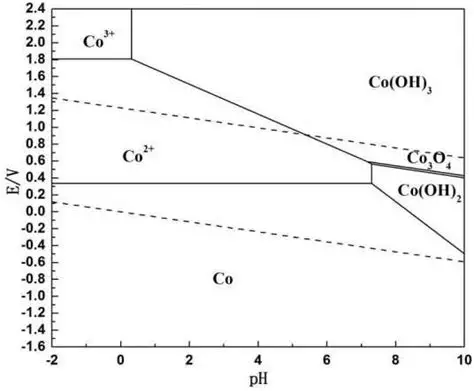
\includegraphics[width=0.62\textwidth]{pourbaix-co.png}
  \caption{钴的电势--$\mathrm{pH}$ 图（普贝图）}
  \label{fig:pourbaix-co}
\end{figure}

第二种是弗罗斯特图，以氧化数为横轴、$nE^\theta$ 为纵轴。图上相邻两点连线的斜率对应步进电势，凹点处对应的物种容易发生歧化，凸点则对应归中。图~\ref{fig:frost-mn} 是锰的弗罗斯特图。

\begin{figure}[H]
  \centering
  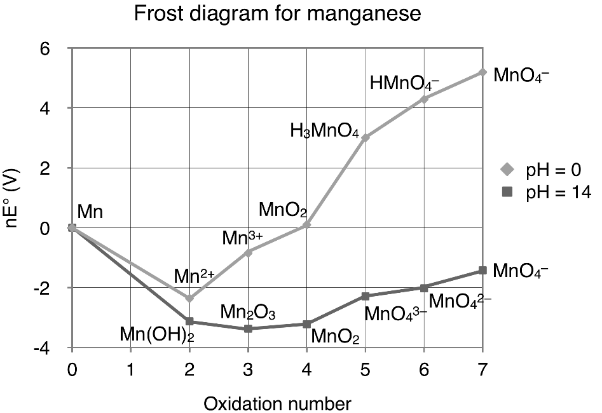
\includegraphics[width=0.68\textwidth]{frost-mn.png}
  \caption{锰的弗罗斯特图}
  \label{fig:frost-mn}
\end{figure}

第三种是拉提莫图，把同一元素各氧化态按从高到低的顺序排成一行，并在相邻物种之间的箭头上标出标准电极电势。例如氯的拉提莫图为
\begin{equation}
\ce{ClO4-}\xrightarrow{+0.37}\ce{ClO3-}\xrightarrow{+0.30}\ce{ClO2-}
\xrightarrow{+0.68}\ce{ClO-}\xrightarrow{+0.42}\ce{Cl2}
\xrightarrow{+1.89}\ce{Cl-}.
\end{equation}
拉提莫图最能直接反映不同氧化态之间的转化趋势：若某物种右侧的电势大于左侧，它便倾向于歧化。熟悉一个元素的氧化还原化学，往往就是从这张图开始的。注意图中各电势均为标准状态下的数值。

\section{化学反应动力学}

热力学只告诉我们反应的终点在哪里，却不告诉我们到达终点需要多久。动力学的基本假设是碰撞理论：只有能量足够、取向正确的分子相遇，才能越过过渡态，反应物才转化为产物。要把“能量足够”与“取向正确”写成定量表达式，先需要统计分布这个工具。

\subsection{配分函数与玻尔兹曼分布}

设有 $M$ 个可区分的系统（例如定域子系统），处于能级 $E_i$ 的系统有 $M_i$ 个，则总系统数与总能量满足
\begin{equation}
\sum_i M_i=M,\qquad \sum_i M_iE_i=E .
\end{equation}
由等概率原理，每一种微观分配方式出现的概率相同。把 $M$ 个可区分的系统分配到各能级，能级 $i$ 上放 $M_i$ 个，分配方式数为
\begin{equation}
\Omega=\frac{M!}{\prod_i M_i!}.
\end{equation}
这里分子上的 $M!$ 是全排列数，分母上的 $M_i!$ 是为了消除同一能级内部交换带来的重复计数——这正是麦克斯韦--玻尔兹曼统计的处理方式。系统处于某一宏观态的概率与该宏观态的 $\Omega$ 成正比：
\begin{equation}
P_i=\frac{\Omega_i}{\Omega_{\mathrm{all}}}.
\end{equation}

平衡分布对应 $\Omega$ 最大的那种分配。为此对 $\ln\Omega$ 求极值。当 $x$ 很大时有斯特林近似
\begin{equation}
\ln x!\approx x\ln x-x,
\end{equation}
于是
\begin{equation}
\ln\Omega\approx M\ln M-M-\sum_i\left(M_i\ln M_i-M_i\right)
=M\ln M-\sum_i M_i\ln M_i .
\end{equation}
其中 $M\ln M$ 为常数，求最大值等价于求 $\sum_i M_i\ln M_i$ 的最小值。约束条件为
\begin{equation}
\varphi_1=\sum_i M_i-M=0,\qquad
\varphi_2=\sum_i E_iM_i-E=0 .
\end{equation}
引入拉格朗日乘子 $\alpha$、$\beta$，构造
\begin{equation}
L=\ln\Omega-\alpha\left(\sum_i M_i-M\right)
-\beta\left(\sum_i E_iM_i-E\right).
\end{equation}
把 $M_i$ 当作连续变量求偏导并令其为零：
\begin{equation}
\frac{\partial L}{\partial M_i}
=-\ln M_i-1-\alpha-\beta E_i=0,
\end{equation}
解得
\begin{equation}
\ln M_i=-1-\alpha-\beta E_i,
\qquad
M_i=Ae^{-\beta E_i}.
\end{equation}
由第一个约束定出 $A$：
\begin{equation}
A\sum_i e^{-\beta E_i}=M
\quad\Longrightarrow\quad
A=\frac{M}{Z},
\end{equation}
其中定义配分函数
\begin{equation}
Z=\sum_i e^{-\beta E_i}.
\end{equation}
于是平衡分布为
\begin{equation}
M_i=\frac{M}{Z}e^{-\beta E_i}.
\end{equation}
再由第二个约束确定 $\beta$。注意到
\begin{equation}
-\frac{\partial Z}{\partial\beta}=\sum_i E_i e^{-\beta E_i},
\end{equation}
因此
\begin{equation}
-M\frac{\partial\ln Z}{\partial\beta}=E .
\end{equation}
与热力学中内能的统计表达式对比，可定出
\begin{equation}
\beta=\frac{1}{k_{\mathrm B}T}.
\end{equation}
至此得到完整的玻尔兹曼分布
\begin{equation}
M_i=\frac{M}{Z}e^{-E_i/k_{\mathrm B}T},
\qquad
Z=\sum_i e^{-E_i/k_{\mathrm B}T}.
\end{equation}
配分函数是统计力学的核心量：系统的所有热力学性质都可以由它导出。

\subsection{碰撞理论与速率方程}

对一般反应 $aA+bB\to cC+dD$，总反应可分解为若干基元反应。以基元反应 $mA+nB\to eE$ 为例，按碰撞理论，速率取决于具有足够活化能的 $A$、$B$ 分子相遇的数目。能级 $E_i$ 上的分子数为 $M_i=Ae^{-E_i/k_{\mathrm B}T}$，而对固定系统配分函数 $Z$ 是常数，因此处于活化态的概率为
\begin{equation}
P=\frac{M}{Z}e^{-E_i/k_{\mathrm B}T}.
\end{equation}
分子相遇还需取向合适，引入取向因子 $f$，则有效碰撞的概率正比于
\begin{equation}
f\,\frac{[A]^m[B]^n}{Z_A^mZ_B^n}\,
e^{-(mE_A+nE_B)/k_{\mathrm B}T}.
\end{equation}
再引入过渡态的坍缩修正因子 $f^*$，反应速率可写为
\begin{equation}
v=ff^*\,\frac{[A]^m[B]^n}{Z_A^mZ_B^n}\,
e^{-(mE_A+nE_B)/k_{\mathrm B}T}.
\end{equation}
对固定反应，配分函数可由分子参数算出，温度是唯一可调的变量，活化能则是唯一的未知量。于是上式可简记为
\begin{equation}
v=A\,e^{-E_a/k_{\mathrm B}T}[A]^m[B]^n,
\end{equation}
即
\begin{equation}
v=k[A]^m[B]^n,\qquad
k=A\,e^{-E_a/k_{\mathrm B}T}.
\end{equation}
这就是质量作用定律。反应级数为 $m+n$，即各反应物浓度幂指数之和。

实验上通常先测不同温度下的速率常数，再求活化能。对速率常数取对数得
\begin{equation}
\ln k=\ln A-\frac{E_a}{k_{\mathrm B}T}.
\end{equation}
用两组数据 $(T_1,k_1)$、$(T_2,k_2)$ 相减，得
\begin{equation}
\ln\frac{k_1}{k_2}
=-\frac{E_a}{k_{\mathrm B}}\left(\frac{1}{T_1}-\frac{1}{T_2}\right).
\end{equation}
因此以 $\ln k$ 对 $1/T$ 作图，斜率为 $-E_a/k_{\mathrm B}$，由斜率即可求出活化能，截距给出指前因子 $A$。

对 $m+n$ 级反应，速率方程常写成
\begin{equation}
v=-\frac{dc}{dt}=k\,c^{m+n},
\end{equation}
其中 $c$ 为按化学计量关系合并后的统一浓度变量。分离变量并积分，得
\begin{equation}
\frac{c^{1-(m+n)}}{1-(m+n)}=kt+C,
\qquad (m+n\neq1)
\end{equation}
由此可由浓度随时间的变化反推反应级数与速率常数。对一级反应，积分结果为指数衰减，这是后面讨论放射性衰变与配合物取代反应的基础。

\newpage


% ---- chunk ch1_4 : 1.3 介观物理模型（顶替缺失的 ch1_3，标题一致） ----



\section{介观物理模型：原子、分子与配合物}

前两节讨论的是宏观的热力学与动力学，本节把尺度缩小到原子与分子，回答三个层层递进的问题：电子在原子核周围如何排布，原子之间如何成键，多个原子与配体又如何组成具有一定空间构型的配合物。这条线索从单个电子的波函数一直延伸到配合物的能级分裂，构成了后面理解各区元素结构性质的理论骨架。

\subsection{从原子光谱到分子间作用力}

在人类还无法直接观测原子的年代，关于原子结构的知识几乎全部来自光谱。1888 年，里德伯从氢原子光谱的经验规律中总结出
\begin{equation}
\tilde{\nu}=R\left(\frac{1}{n_1^2}-\frac{1}{n_2^2}\right),
\end{equation}
其中 $\tilde{\nu}$ 为波数，$R$ 为里德伯常数，$n_1<n_2$ 为正整数。这条经验公式后来成为玻尔原子模型最有力的证据之一：它说明原子内部只允许某些分立的能量状态。

从原子到分子，首先遇到的是电荷分布是否对称的问题。若分子中正、负电荷中心重合，电偶极矩为零，称为\textbf{非极性分子}；若二者不重合，电偶极矩不为零，称为\textbf{极性分子}。电偶极矩的定义为
\begin{equation}
\boldsymbol{\mu}=q\mathbf{d},
\end{equation}
其中 $q$ 为极上电荷，$\mathbf{d}$ 为正负电荷中心之间的矢量。偶极矩的大小反映分子极性的强弱，方向习惯上由正电荷指向负电荷。

分子靠近时产生的偶极有三种来源。极性分子本身固有的偶极称为\textbf{固有偶极}（永久偶极）；非极性分子相互靠近时，电子与原子核的瞬时相对位移使正负电荷中心暂时分离，产生\textbf{瞬时偶极}；极性分子与非极性分子靠近时，后者的电荷中心在前者的电场中被拉开，产生\textbf{诱导偶极}。三种偶极对应三种分子间作用力，统称范德华引力：

\begin{itemize}
  \item \textbf{取向力}：固有偶极之间因取向而产生的吸引，强极性分子之间以此为主；
  \item \textbf{诱导力}：固有偶极与诱导偶极之间的相互作用，存在于极性--非极性以及极性--极性分子之间，通常较小；
  \item \textbf{色散力}：瞬时偶极诱导邻近分子产生瞬时偶极，异极相吸。一切分子之间都存在色散力，而且对大多数分子而言，色散力是分子间作用力的主要成分。
\end{itemize}

与分子间力平行的另一对概念是离子极化。离子使邻近离子发生形变的能力称为\textbf{极化能力}：离子半径越小、电荷越高，极化能力越强。离子自身被外加电场形变的能力称为\textbf{变形性}：离子半径越大、电荷越低，变形性越强。这两条看似简单的规律，后面在解释离子键向共价键过渡、以及某些化合物颜色加深时会反复用到。

\subsection{原子模型}

\subsubsection{基态氢原子轨道波函数}

单电子原子的定态行为由薛定谔方程描述：
\begin{equation}
\frac{\partial^2\psi}{\partial x^2}
+\frac{\partial^2\psi}{\partial y^2}
+\frac{\partial^2\psi}{\partial z^2}
+\frac{2m}{\hbar^2}\left(E-V\right)\psi=0 .
\end{equation}
对中心力场中的电子，直角坐标并不方便，应换到球坐标。拉普拉斯算符在球坐标下写作
\begin{equation}
\nabla^2\psi=\frac{1}{r^2\sin\theta}\left[
\sin\theta\frac{\partial}{\partial r}\left(r^2\frac{\partial\psi}{\partial r}\right)
+\frac{\partial}{\partial\theta}\left(\sin\theta\frac{\partial\psi}{\partial\theta}\right)
+\frac{1}{\sin\theta}\frac{\partial^2\psi}{\partial\varphi^2}\right].
\end{equation}
氢原子核的势能为 $V=-Ze^2/(4\pi\varepsilon_0r)$，代回原方程得
\begin{equation}
\frac{1}{r^2\sin\theta}\left[
\sin\theta\frac{\partial}{\partial r}\left(r^2\frac{\partial}{\partial r}\right)
+\frac{\partial}{\partial\theta}\left(\sin\theta\frac{\partial}{\partial\theta}\right)
+\frac{1}{\sin\theta}\frac{\partial^2}{\partial\varphi^2}\right]\psi
+\frac{2m}{\hbar^2}\left(E+\frac{Ze^2}{4\pi\varepsilon_0r}\right)\psi=0 .
\end{equation}

由于势场是球对称的，可以尝试分离变量：
\begin{equation}
\psi(r,\theta,\varphi)=R(r)\,\Theta(\theta)\,\Phi(\varphi).
\end{equation}
代入后两边同乘 $r^2\sin^2\theta/(R\Theta\Phi)$，可以把含 $\varphi$ 的项单独移到等式一侧：
\begin{equation}
\frac{1}{R}\frac{1}{r^2}\frac{d}{dr}\left(r^2\frac{dR}{dr}\right)
+\frac{1}{\Theta}\frac{1}{r^2\sin\theta}\frac{d}{d\theta}\left(\sin\theta\frac{d\Theta}{d\theta}\right)
+\frac{2m}{\hbar^2}\left(E+\frac{Ze^2}{4\pi\varepsilon_0r}\right)
=-\frac{1}{\Phi\sin^2\theta}\frac{d^2\Phi}{d\varphi^2}.
\end{equation}
等式左边只含 $r$、$\theta$，右边只含 $\varphi$，故两边必等于同一常数。记为 $m^2$，即得方位角方程
\begin{equation}
\frac{d^2\Phi}{d\varphi^2}+m^2\Phi=0 .
\end{equation}
剩余的径向与极角部分可以再分离一次。把含 $\Theta$ 的项归到一边，令其等于 $l(l+1)$，于是得到极角方程与径向方程：
\begin{equation}
\frac{1}{\sin\theta}\frac{d}{d\theta}\left(\sin\theta\frac{d\Theta}{d\theta}\right)
+\left[l(l+1)-\frac{m^2}{\sin^2\theta}\right]\Theta=0,
\end{equation}
\begin{equation}
\frac{1}{r^2}\frac{d}{dr}\left(r^2\frac{dR}{dr}\right)
+\left[\frac{2m}{\hbar^2}\left(E+\frac{Ze^2}{4\pi\varepsilon_0r}\right)-\frac{l(l+1)}{r^2}\right]R=0 .
\end{equation}

三个方程依次求解。第一个方程最简单，其归一化解为
\begin{equation}
\Phi_m(\varphi)=\frac{1}{\sqrt{2\pi}}e^{im\varphi}.
\end{equation}
单值性要求 $\Phi(\varphi+2\pi)=\Phi(\varphi)$，因此 $m$ 必须为整数。

第二个方程先令 $m=0$，并作代换 $x=\cos\theta$，化为勒让德方程
\begin{equation}
(1-x^2)\frac{d^2\Theta}{dx^2}-2x\frac{d\Theta}{dx}
+\left[l(l+1)-\frac{m^2}{1-x^2}\right]\Theta=0 .
\end{equation}
设解为幂级数 $\Theta(x)=\sum_{k=0}^{\infty}a_k x^k$，代入后比较同次幂系数，得到递推关系
\begin{equation}
a_{k+2}=\frac{k(k+1)-\lambda}{(k+2)(k+1)}a_k,
\end{equation}
其中 $\lambda$ 是与分离常数有关的参数。若级数在 $k\to\infty$ 时不截断，则 $a_{k+2}\approx a_k$，级数行为近似于 $\sum x^k/k^2$，在 $x=\pm1$（即 $\theta=0,\pi$）处发散，波函数在极点失去物理意义。为保证波函数有限且平方可积，级数必须在某一阶 $k_{\max}$ 之后截断，即存在 $k$ 使 $a_{k+2}=0$。这要求 $\lambda=l(l+1)$，其中 $l$ 为非负整数。截断后 $\Theta(x)$ 退化为多项式，即勒让德多项式 $P_l(x)$。

对于 $m\neq0$ 的情形，需由勒让德多项式构造连带勒让德函数
\begin{equation}
P_l^m(x)=(-1)^m(1-x^2)^{m/2}\frac{d^m}{dx^m}P_l(x),
\qquad m\geq0 .
\end{equation}

第三个是径向方程。先把第一项展开：
\begin{equation}
\frac{1}{r^2}\frac{d}{dr}\left(r^2\frac{dR}{dr}\right)
=\frac{d^2R}{dr^2}+\frac{2}{r}\frac{dR}{dr},
\end{equation}
代入后引入玻尔半径与里德伯能量
\begin{equation}
a_0=\frac{4\pi\varepsilon_0\hbar^2}{me^2},
\qquad
E_0=\frac{me^4}{2(4\pi\varepsilon_0)^2\hbar^2},
\end{equation}
并定义无量纲变量
\begin{equation}
\rho=\frac{Zr}{a_0},\qquad \epsilon=\frac{E}{E_0}.
\end{equation}
径向方程化为
\begin{equation}
\frac{d^2R}{d\rho^2}+\frac{2}{\rho}\frac{dR}{d\rho}
+\left[\epsilon+\frac{2}{\rho}-\frac{l(l+1)}{\rho^2}\right]R=0 .
\end{equation}
令 $R(\rho)=\rho^l e^{-\rho/n}L(\rho)$，其中 $n$ 为待定的主量子数，代入后可化为拉盖尔方程，其解为连带拉盖尔多项式
\begin{equation}
L_n^{\alpha}(\rho)=\frac{\rho^{-\alpha}e^{\rho}}{n!}
\frac{d^n}{d\rho^n}\left(\rho^{n+\alpha}e^{-\rho}\right).
\end{equation}
为保证波函数在 $r\to\infty$ 时收敛，能量必须量子化：
\begin{equation}
E_n=-\frac{Z^2E_0}{n^2}
=-\frac{Z^2}{n^2}\cdot\frac{me^4}{2(4\pi\varepsilon_0)^2\hbar^2},
\qquad n=l+1,l+2,\dots
\end{equation}

综合三部分，完整的轨道波函数为
\begin{equation}
\psi_{n,l,m}(r,\theta,\varphi)
=R_{n,l}(r)\,\Theta_{l,m}(\theta)\,\Phi_m(\varphi).
\end{equation}
三个量子数的物理意义也随之明确：主量子数 $n$ 决定能层与轨道能量；角量子数 $l=0,1,2,\dots,n-1$ 决定轨道的形状；磁量子数 $m=-l,\dots,+l$ 决定轨道在空间中的取向。

\subsubsection{原子轨道波函数}

把三部分合起来看，
\begin{equation}
\Phi_m(\varphi)=\frac{1}{\sqrt{2\pi}}e^{im\varphi},\qquad
\Theta_{l,m}(\theta)=P_l^m(\cos\theta),\qquad
R_{n,l}(r)\propto\rho^l e^{-\rho/n}L_{n-l-1}^{2l+1}(\rho).
\end{equation}
任何单电子原子的轨道都具有相似的形式，因为电子感受到的都是球对称势场；改变原子核电荷或选取不同量子数，只是改变了参数。

多电子原子则不同。电子之间的相互作用使势场不再是严格的球对称场，无法用上述解析解直接描述。常用的处理是引入屏蔽常数 $\sigma$，把内层电子对核电荷的削弱折算进去，用有效核电荷
\begin{equation}
Z^*=Z-\sigma
\end{equation}
代替真实的 $Z$，再把体系近似当作类氢原子处理。这个近似虽然粗糙，却足以解释能级交错、原子半径变化与电离能趋势等大量现象。

\subsection{分子轨道模型}

分子轨道模型是原子轨道模型的自然推广：先写出氢分子的哈密顿量，再设法近似求解。氢分子含两个电子和两个核 $A$、$B$，哈密顿量为
\begin{equation}
\begin{aligned}
H=&-\frac{\hbar^2}{2m_e}\left(\nabla_1^2+\nabla_2^2\right)
-\frac{e^2}{4\pi\varepsilon_0}\left(\frac{1}{r_{1A}}+\frac{1}{r_{1B}}+\frac{1}{r_{2A}}+\frac{1}{r_{2B}}\right)\\
&+\frac{e^2}{4\pi\varepsilon_0 r_{12}}
+\frac{e^2}{4\pi\varepsilon_0 R_{AB}},
\end{aligned}
\end{equation}
其中第一行依次是两电子的动能与电子--核吸引势能，第二行是电子--电子排斥与核--核排斥。由于 $1/r_{12}$ 把两个电子的坐标耦合在一起，方程无法精确解析求解，只能借助近似方法。无论采用哪种近似，求解过程大体都遵循四步：

\begin{enumerate}
  \item 建立试探波函数 $\Psi=c_1\Psi_1+c_2\Psi_2$；
  \item 用变分法求能量泛函 $E=\langle\Psi|H|\Psi\rangle/\langle\Psi|\Psi\rangle$，得到久期方程，解出使能量最低的系数 $c_1$、$c_2$；
  \item 代入系数求能量，并由归一化条件定出归一化系数；
  \item 得到完整的轨道模型。
\end{enumerate}

\subsubsection{化学键模型}

价键模型假设成键的两个电子分属两个原子，波函数写成两种分配方式的线性组合：
\begin{equation}
\Psi=c_1\,\phi_A(1)\phi_B(2)+c_2\,\phi_A(2)\phi_B(1).
\end{equation}
按变分法，能量泛函为
\begin{equation}
E=\frac{\langle\Psi|H|\Psi\rangle}{\langle\Psi|\Psi\rangle}
=\frac{\iint\Psi^*H\Psi\,d\tau_1d\tau_2}
{\iint\Psi^*\Psi\,d\tau_1d\tau_2}.
\end{equation}
由对称性，两种分配方式权重相同，即 $c_1=c_2$。分别代入对称与反对称组合，归一化系数为
\begin{equation}
N_-=\frac{1}{\sqrt{2-2S_{12}}},\qquad
N_+=\frac{1}{\sqrt{2+2S_{12}}}.
\end{equation}
相应的能量为
\begin{equation}
E_-=\frac{H_{11}-H_{12}}{1-S_{12}},\qquad
E_+=\frac{H_{11}+H_{12}}{1+S_{12}}.
\end{equation}
其中出现的几个积分各有名称与含义：
\begin{itemize}
  \item 库仑积分 $Q=H_{11}=\iint\phi_A(1)\phi_B(2)\,H\,\phi_A(1)\phi_B(2)\,d\tau_1d\tau_2$；
  \item 交换积分 $J=H_{12}=\iint\phi_A(1)\phi_B(2)\,H\,\phi_A(2)\phi_B(1)\,d\tau_1d\tau_2$；
  \item 重叠积分 $S=\int\phi_A\phi_B\,d\tau$，以及 $S_{12}=\iint\phi_A(1)\phi_B(2)\phi_A(2)\phi_B(1)\,d\tau_1d\tau_2$，在简单情形下 $S_{12}=S^2$。
\end{itemize}
于是得到一对成键与反键轨道：
\begin{equation}
\Psi_+=\frac{1}{\sqrt{2+2S_{12}}}\left[\phi_A(1)\phi_B(2)+\phi_A(2)\phi_B(1)\right],
\qquad E_+=\frac{H_{11}+H_{12}}{1+S_{12}},
\end{equation}
\begin{equation}
\Psi_-=\frac{1}{\sqrt{2-2S_{12}}}\left[\phi_A(1)\phi_B(2)-\phi_A(2)\phi_B(1)\right],
\qquad E_-=\frac{H_{11}-H_{12}}{1-S_{12}}.
\end{equation}
两轨道的能量差来自交换积分与重叠积分，前者提供主要的稳定化，后者修正其大小。价键模型因此得到一个重要结论：共价键的稳定化能本质上来源于电子的交换作用。

\subsubsection{杂化轨道模型}

价键模型能解释双原子分子，却难以说明甲烷的正四面体构型。杂化轨道模型的处理是：同一原子中能量相近的原子轨道先线性组合成一组新的等价轨道，再由这些杂化轨道与其它原子成键。以 $\mathrm{sp^3}$ 杂化为例，一个 $s$ 轨道与三个 $p$ 轨道等性混合，每个杂化轨道写作
\begin{equation}
h_i=a_i\phi_{1s}+b_i\phi_{2p_x}+c_i\phi_{2p_y}+d_i\phi_{2p_z}.
\end{equation}
系数由归一化与正交性条件确定：
\begin{equation}
\langle h_i|h_i\rangle=a_i^2+b_i^2+c_i^2+d_i^2=1,
\qquad
\langle h_i|h_j\rangle=a_ia_j+b_ib_j+c_ic_j+d_id_j=0 .
\end{equation}
四条等价轨道要彼此正交且完全等价，解为
\begin{equation}
|a_i|=|b_i|=|c_i|=|d_i|=\frac{1}{2},
\end{equation}
正负号的排布决定了四个杂化轨道分别指向正四面体的四个顶点。这就解释了 $\mathrm{CH_4}$ 的键角为 $109.5^\circ$。

\subsubsection{分子轨道模型}

分子轨道模型不预先指定电子属于哪个原子，而是直接把整个分子的波函数写成原子轨道的线性组合。对双原子分子，取两个原子轨道 $\phi_A$、$\phi_B$，组合为
\begin{equation}
\Psi=c_1\phi_A+c_2\phi_B,\qquad
\Psi^*=c_1\phi_A-c_2\phi_B .
\end{equation}
以氢分子为例，两个基轨道都是 $1s$ 轨道：
\begin{equation}
\phi_A(\mathbf{r})=\frac{1}{\sqrt{\pi a_0^3}}e^{-r_A/a_0},
\qquad
\phi_B(\mathbf{r})=\frac{1}{\sqrt{\pi a_0^3}}e^{-r_B/a_0}.
\end{equation}
把试探轨道代入变分能量泛函：
\begin{equation}
E=\frac{\langle\Psi|H|\Psi\rangle}{\langle\Psi|\Psi\rangle}
=\frac{c_1^2H_{AA}+2c_1c_2H_{AB}+c_2^2H_{BB}}
{c_1^2S_{AA}+2c_1c_2S_{AB}+c_2^2S_{BB}}.
\end{equation}
各积分的含义为：库仑积分 $H_{AA}=\int\phi_AH\phi_A\,d\tau$、$H_{BB}=\int\phi_BH\phi_B\,d\tau$，由对称性 $H_{AA}=H_{BB}=\alpha$；共振积分 $H_{AB}=\int\phi_AH\phi_B\,d\tau=H_{BA}=\beta$；重叠积分 $S_{AB}=\int\phi_A\phi_B\,d\tau=S$；归一化积分 $S_{AA}=S_{BB}=1$。

令能量对两个系数的偏导为零，
\begin{equation}
\frac{\partial E}{\partial c_1}=\frac{\partial E}{\partial c_2}=0,
\end{equation}
得到久期方程
\begin{equation}
\begin{cases}
(H_{AA}-E)c_1+(H_{AB}-ES_{AB})c_2=0,\\
(H_{BA}-ES_{BA})c_1+(H_{BB}-E)c_2=0,
\end{cases}
\end{equation}
有非零解的条件是系数行列式为零：
\begin{equation}
\begin{vmatrix}
H_{AA}-E & H_{AB}-ES_{AB}\\
H_{BA}-ES_{BA} & H_{BB}-E
\end{vmatrix}=0 .
\end{equation}
代入 $\alpha$、$\beta$、$S$，并利用对称性，行列式化为
\begin{equation}
(\alpha-E)^2-(\beta-ES)^2=0,
\end{equation}
解得
\begin{equation}
E_-=\frac{\alpha-\beta}{1-S},\qquad
E_+=\frac{\alpha+\beta}{1+S}.
\end{equation}
分别代回久期方程，得
\begin{equation}
\Psi_+=\frac{1}{\sqrt{2+2S}}\left(\phi_A+\phi_B\right),
\qquad E_+=\frac{\alpha+\beta}{1+S},
\end{equation}
\begin{equation}
\Psi_-=\frac{1}{\sqrt{2-2S}}\left(\phi_A-\phi_B\right),
\qquad E_-=\frac{\alpha-\beta}{1-S}.
\end{equation}
$E_+$ 低于原来的原子轨道能级，对应成键轨道；$E_-$ 高于原能级，对应反键轨道；两者的能量差为 $2\beta/(1-S^2)$。与价键模型相比，分子轨道模型的显著优势在于它允许电子占据非键或反键轨道，因此能自然地解释分子中单电子的存在、以及氧分子的顺磁性等现象。

\subsection{配合物}

配位化合物由中心原子（或离子）与若干配体通过配位键结合而成。中心原子提供空轨道，配体提供孤对电子，二者形成具有一定空间构型的整体。

\subsubsection{命名与异构}

配合物的命名遵循以下顺序：

\begin{itemize}
  \item 先无机后有机；
  \item 先阴离子，后阳离子和中性分子；
  \item 同类配体按字母顺序排列；
  \item 配位原子相同时，原子数少的写在前面；
  \item 原子数也相同时，按与配位原子直接相连的其它原子在字母表中的次序排列。
\end{itemize}

配合物的异构分为两大类。\textbf{结构异构}包括：解离异构（内外界交换成分）、配位异构（内界之间交换配体）、键合异构（同一配体以不同配位原子配位）与配体异构（配体本身互为异构体）。\textbf{立体异构}包括：几何异构（如 $\mathrm{Ma_3b_3}$、$\mathrm{Ma_2b_2}$、$\mathrm{Mabc_2}$、$\mathrm{Mabcd}$ 等类型）与旋光异构（手性，两种对映体不能重合）。

\subsubsection{晶体场理论}

\paragraph{晶体场模型}

中心原子的价层轨道杂化方式不同，所成键的强度也不同。若只用外层轨道 $(ns)(np)(nd)$ 杂化，得到的是\textbf{外轨型}配合物，电价配键较弱；若动用内层 $(n-1)d$ 轨道参与杂化，得到\textbf{内轨型}配合物，共价配键较强。

晶体场模型从静电作用出发：配体被看作点电荷或偶极子，它们对中心原子的五个简并 $d$ 轨道产生不同程度的排斥，使能级发生分裂。分裂后体系能量降低，所释放的能量即分裂能 $\Delta$。与此同时，电子在轨道间重新排布需要克服成对能 $P$，即把两个电子挤进同一轨道所需付出的能量。二者竞争决定了电子的排布方式：

\begin{itemize}
  \item 当 $\Delta>P$ 时，电子倾向于成对占据低能轨道，形成\textbf{低自旋}态；
  \item 当 $\Delta<P$ 时，电子倾向于分占各轨道并保持自旋平行，形成\textbf{高自旋}态。
\end{itemize}

内轨型配合物的分裂能通常大于外轨型，因此内轨型多为低自旋，外轨型多为高自旋。配合物的自旋状态可由磁矩判断：
\begin{equation}
\mu=\sqrt{n(n+2)}\,\mu_{\mathrm B},
\end{equation}
其中 $n$ 为未成对电子数，$\mu_{\mathrm B}$ 为玻尔磁子。测得磁矩即可反推 $n$，从而判断高自旋还是低自旋。

\paragraph{八面体场的对称性分析}

晶体场理论的定量处理是微扰理论的一个漂亮范例。先写出未受微扰的哈密顿算符及其本征方程：
\begin{equation}
H_0\phi=E_0\phi .
\end{equation}
配体场作为微扰加入：
\begin{equation}
H=H_0+V,
\end{equation}
其中 $V$ 是晶体场引起的势能变化。由于晶体场模型是纯静电模型，势能全部来自配体：
\begin{equation}
V=\frac{q}{4\pi\varepsilon_0|\mathbf{r}-\mathbf{R}|},
\end{equation}
$\mathbf{r}$ 为电子位矢，$\mathbf{R}$ 为配体位矢。把 $V$ 按球谐函数展开：
\begin{equation}
V(r,\theta,\varphi)=\sum_{k=0}^{\infty}\sum_{m=-k}^{k}
A_{k,m}\,r^k\,Y_k^m(\theta,\varphi),
\end{equation}
其中展开系数 $A_{k,m}$ 由配体的几何构型决定，正是它区分了四面体、八面体与平面四边形等不同场。

中心原子的五个简并 $d$ 轨道为
\begin{equation}
\phi_1,\dots,\phi_5=d_{xy},\,d_{xz},\,d_{yz},\,d_{z^2},\,d_{x^2-y^2}.
\end{equation}
微扰后，一级能量修正由久期方程给出：
\begin{equation}
\det\left|\langle\phi_i|V|\phi_j\rangle-E'\delta_{ij}\right|=0 .
\end{equation}
这是五个轨道之间的二十五个矩阵元，直接计算极为繁琐。对称性可以大幅简化：以八面体场 $O_h$ 为例，$O_h$ 群是旋转群 $O$（24 个操作）与反演群 $\{E,i\}$ 的直积，
\begin{equation}
O_h=O\times\{E,i\}.
\end{equation}
其中 $E$ 为恒等操作，$i$ 为中心反演 $(x,y,z)\mapsto(-x,-y,-z)$。$d$ 轨道在反演下为偶函数（记为 $g$），因此只需考虑 $O$ 群的 24 个旋转操作。

对称操作前后物理规律不变，这意味着五个 $d$ 轨道构成 $O$ 群的一个五维表示。若一个矩阵与所有旋转操作对易，则它与整个群的表示矩阵可以同时对角化。我们希望把可约表示分解为不可约表示，也就是把五个轨道分成若干组、每组内部按同一变换规律变化。判据是特征标，即表示矩阵的迹：在该操作下保持自身方向的基函数贡献 1 到对角元，被混入其它轨道的基函数不贡献。

$O$ 群的五类操作及其在 $d$ 轨道基上的特征标为：
\begin{itemize}
  \item $E$：所有轨道不变，$\chi(E)=5$；
  \item $C_3$：沿体对角线旋转 $120^\circ$，$\chi(C_3)=-1$；
  \item $C_4$：沿面心轴旋转 $90^\circ$，$\chi(C_4)=-1$；
  \item $C_2$：沿面心轴旋转 $180^\circ$，$\chi(C_2)=1$；
  \item $C_2'$：绕对棱中点轴旋转 $180^\circ$，$\chi(C_2')=1$。
\end{itemize}
对照 $O$ 群的特征标表（表~\ref{tab:O-character}），可以验证这组特征标恰好分解为 $E_g$ 与 $T_{2g}$ 两个不可约表示之和：
\begin{equation}
\chi=E_g+T_{2g}.
\end{equation}

\begin{table}[H]
\centering
\caption{$O$ 群的特征标表}
\label{tab:O-character}
\renewcommand{\arraystretch}{1.15}
\begin{tabular}{@{}lccccc@{}}
\toprule
$O$ & $E$ & $8C_3$ & $3C_2$ & $6C_4$ & $6C_2'$ \\
\midrule
$A_1$ & 1 & 1 & 1 & 1 & 1 \\
$A_2$ & 1 & 1 & 1 & $-1$ & $-1$ \\
$E$   & 2 & $-1$ & 2 & 0 & 0 \\
$T_1$ & 3 & 0 & $-1$ & 1 & $-1$ \\
$T_2$ & 3 & 0 & $-1$ & $-1$ & 1 \\
\bottomrule
\end{tabular}
\end{table}

由舒尔引理，若一个算符与群的所有操作对易，则它在该不可约表示的子空间内只能是常数乘以单位矩阵。于是势能矩阵在 $T_{2g}$ 与 $E_g$ 两个子空间内分别退化为常数，整个矩阵化简为
\begin{equation}
V=\operatorname{diag}\bigl(
\underbrace{\alpha,\alpha,\alpha}_{T_{2g}},\;
\underbrace{\beta,\beta}_{E_g}\bigr),
\end{equation}
其中三个 $\alpha$ 对应 $t_{2g}$ 组（$d_{xy}$、$d_{xz}$、$d_{yz}$），两个 $\beta$ 对应 $e_g$ 组（$d_{z^2}$、$d_{x^2-y^2}$）。

现在只需确定 $\alpha$ 与 $\beta$ 之差。定义分裂能
\begin{equation}
\Delta_O=\alpha-\beta=10Dq,
\end{equation}
并把能级重心取为零点，则由重心守恒得
\begin{equation}
E_{t_{2g}}=3\alpha+2\beta=0
\quad\Longrightarrow\quad
\alpha=-4Dq,\qquad \beta=+6Dq .
\end{equation}
可见八面体场中五个简并的 $d$ 轨道分裂为两组：$t_{2g}$ 组能量降低 $4Dq$，$e_g$ 组能量升高 $6Dq$，二者相差 $10Dq$。分裂图像如图~\ref{fig:oct-splitting} 所示。

\begin{figure}[H]
  \centering
  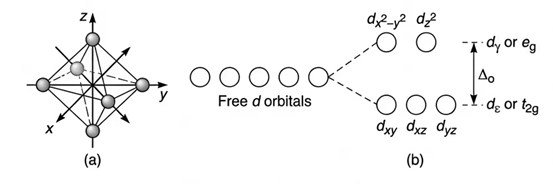
\includegraphics[width=0.85\textwidth]{Oct.png}
  \caption{八面体场中 $d$ 轨道的能级分裂}
  \label{fig:oct-splitting}
\end{figure}

四面体场与平面四边形场可用同样的方法处理，只是微扰的对称性不同。四面体场中 $t_2$ 组能量升高、$e$ 组能量降低，分裂图像与八面体场上下颠倒，且分裂能小得多（图~\ref{fig:tet-splitting}）；平面四边形场则分裂得更为复杂（图~\ref{fig:quad-splitting}）。三种场的分裂能相对大小为
\begin{equation}
\Delta_p>\Delta_o>\Delta_t ,
\end{equation}
即平面四边形最大、八面体次之、四面体最小。此外，中心离子的电荷数、所在周期以及配体的场强（即电子排布与配位原子的性质）都会影响分裂能的大小。

\begin{figure}[H]
  \centering
  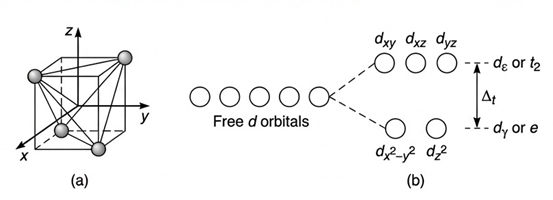
\includegraphics[width=0.85\textwidth]{Tetra.png}
  \caption{四面体场中 $d$ 轨道的能级分裂}
  \label{fig:tet-splitting}
\end{figure}

\begin{figure}[H]
  \centering
  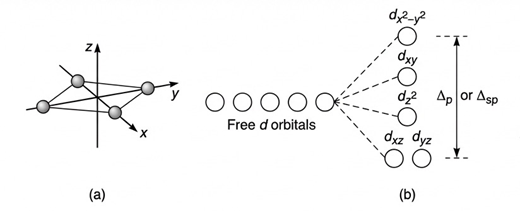
\includegraphics[width=0.85\textwidth]{Quad.png}
  \caption{平面四边形场中 $d$ 轨道的能级分裂}
  \label{fig:quad-splitting}
\end{figure}

\paragraph{晶体场稳定化能}

晶体场稳定化能（CFSE）是体系因能级分裂而额外降低的能量，定义为球形场能量与分裂后能量之差：
\begin{equation}
\mathrm{CFSE}=E_{\mathrm{spherical}}-E_{\mathrm{crystal}}=-E_{\mathrm{crystal}} .
\end{equation}
把电子按高、低自旋规则填入 $t_{2g}$ 与 $e_g$ 轨道，再按各自能量求和，即可得到 CFSE。它直接影响配合物的热力学稳定性、磁性与动力学行为，也是比较不同构型稳定性的重要依据。

\paragraph{姜--泰勒效应}

姜--泰勒效应可以看作一次“对称性自发破缺”：为了获得额外的稳定化能，高对称性的结构会自发畸变为低对称性的结构。

其基本定理是：在非线性多原子分子中，如果某一电子组态是轨道简并的（多个轨道能量相同），则该分子必然发生畸变以解除简并，从而达到更稳定的状态。对理想的八面体配合物，若电子在 $e_g$ 或 $t_{2g}$ 上均匀占据，则结构稳定；若占据不对称，就相当于在某一方向上产生了不平衡的推拉，畸变随之发生。

\begin{itemize}
  \item 最显著的情形是 $e_g$ 的不对称占据：两个简并轨道中一个填满、另一个半满。为降低总能量，$E_g$ 组进一步分裂，八面体沿 $z$ 轴拉长或压扁，形成拉长的八面体场。
  \item $t_{2g}$ 的不对称占据引起较弱的姜--泰勒效应。
  \item 当 $e_g$ 与 $t_{2g}$ 全满、半满或全空时，电子分布对称，不发生姜--泰勒畸变。
\end{itemize}

姜--泰勒畸变不是罕见的例外，而是理解许多过渡金属配合物结构畸变、颜色变化与磁性的关键。它把晶体场理论的静态图像与分子几何的动态调整联系了起来。




% ===== [源文件缺失 ch1：原章首/1.1，源文件已被编译日志覆盖，无法恢复] =====

% ---- chunk ch2 : 第二章 元素化学 2.1 总论 ----

\chapter{元素化学}

本章从总论开始，先给出适用于各区的共同规则，再按 S、P、D 与 DS 分区讨论元素及其化合物的性质。

\section{总论：适用于各区的原理}

本节讨论的不是某一族元素的“特殊小故事”，而是几乎整张周期表都会反复用到的基本思想：电子怎样排布，能级怎样升降，屏蔽怎样改变有效核电荷，离子怎样极化，键型怎样从理想离子键滑向共价键。它们像一组底层规则。后面不论谈 S 区、P 区还是 D 区，只要现象看起来复杂，我们都可以回头问一句：这里究竟是哪一条基本规则在起作用？

\subsection{结构、能级与松紧效应}

松紧效应指原子能层随周期变化呈现“松—紧”交替的趋势，其形成与核电荷增长、屏蔽效应变化、相对论修正及层间补偿的共同作用有关。它在不同分区中的表现并不相同，可概括为两种模式：
\begin{itemize}
  \item 模式A： 对于s区元素，松紧效应呈第二周期松-第三周期紧-...的模式
  \item 模式B：对于p区元素，松紧效应呈第三周期松-第四周期紧-...的模式
\end{itemize}

通常认为，$d$层电子屏蔽不完全会使有效核电荷增加；相对论效应又增强了$s$电子的钻穿与收缩，进一步加强外层电子所受束缚，从而形成“紧”。而前一周期的“紧”又会增强对外层电子的屏蔽，进而在后一周期表现出“松”。
在同一主量子数（同层）下，电子的钻穿能力经验排序为：
\[
\mathrm{s > p > d > f}
\]
钻穿能力越强，电子越可能出现在靠近原子核的区域，受到更大的核吸引；因此对应轨道电子平均能量更低、稳定性更高。

屏蔽效应指内层电子对外层电子感受到的核电荷的削弱。由于同层中不同轨道的钻穿能力不同，其“屏蔽与被屏蔽”表现也不同：
\begin{enumerate}
  \item 对同层电子而言，$s$ 电子钻穿最强，对其他电子的屏蔽贡献通常更明显；$d,f$ 电子钻穿较弱，屏蔽效率较差。
  \item 当过渡元素与后过渡元素参与成键时，$d$ 电子屏蔽不完全可使外层电子感受到较高有效核电荷，进而影响原子半径、电离能与氧化态稳定性。
  \item 需同时考虑“\textbf{钻穿能力差异} + \textbf{屏蔽不完全}”对有效核电荷 $Z_{\mathrm{eff}}$ 的联合作用，才能解释部分非单调变化。
\end{enumerate}

由于有效核电荷的精确计算较为复杂，这里只引入一种常用的经验规则：\textbf{Slater 规则}
\[
Z_{\mathrm{eff}} = Z - S
\]
其中 $Z$ 为核电荷数，$S$ 为屏蔽常数。具体计算可按以下步骤：
\begin{enumerate}
  \item 先按组写电子排布：
  \[(1s)\,(2s,2p)\,(3s,3p)\,(3d)\,(4s,4p)\,(4d)\,(4f)\cdots\]
  \item 对于待求电子是 $ns/np$：
  同组其余电子各记 $0.35$（$1s$ 组内为 $0.30$）；前一层 $(n-1)$ 各记 $0.85$；再内层 $(n-2)$ 及更内层各记 $1.00$。
  \item 对于待求电子是 $nd/nf$：
  同组其余电子各记 $0.35$；其左侧所有电子（含同主量子数的 $ns,np$）一般按 $1.00$ 计；右侧电子不计。
\end{enumerate}

沿族向下可用“松紧效应”辅助理解元素性质变化：通常把高电荷密度、束缚电子更强的一端称为“紧”，其化学行为更偏向氧化性；而电子束缚相对较弱的一端称为“松”，更容易失电子，因而还原性增强。

对于无机化学学习者而言，元素周期律是理解元素性质与变化规律的重要理论框架。然而随着学习的深入，一系列周期反常现象——如碱土金属与硼族电离能反常、铜分族中银元素的特殊性、$p$区含氧酸氧化性的“中间高两端低”等——常以离散知识点形式呈现，缺乏统一且可定量的解释框架。

为服务化学教学，金松寿教授曾提出“松紧效应”这一经验规律；本文在此基础上进一步归纳其原理与应用。通过比较狄拉克方程修正结果与玻尔能级差值，我们发现后者反而更清楚地呈现出“松紧”特征。因此，本文倾向于认为：松紧效应未必首先来自电子相互作用或相对论效应，而可能更根本地源于主量子数$n$与核电荷数$Z$增长之间的结构性不对称。
具体而言，$n$按周期递增，而电子层容量（$2, 8, 18, 32, \ldots$）并不均匀，因而$Z$在层间填充时呈“跳跃式”增长。这种$(Z,n)$增长的不对称，使相邻周期的能级差自然演化为“大—小—大”的交替模式。换言之，许多周期反常并非孤立例外，而是原子结构内在数学关系的外显。

全部计算采用原子单位制（$\hbar=e=m_e=1$）。



氢样原子的玻尔能级，以及在玻尔框架下引入有效核电荷修正后的多电子原子近似能级可表示为
\begin{equation}
E_n^{\mathrm{Bohr}}=-\frac{Z^2}{2n^2},\qquad E_n^{\mathrm{Sch}}=-\frac{Z_{\mathrm{eff}}^2}{2n^2},
\label{eq:bohr_zeff}
\end{equation}
其中$Z_{\mathrm{eff}}$为有效核电荷数，$n$为主量子数，能量单位为$Hartree$（$a.u.$）。



高精度数值解采用Dirac--Fock方法。多电子原子的相对论近似哈密顿量写作
\begin{equation}
H = \sum_i H_D(i) + \frac{1}{2} \sum_{i,j} \left\{ \frac{1}{r_{ij}} + H_B(i,j) \right\},
\end{equation}
其中$H_D(i)$为单电子Dirac哈密顿量：
\begin{equation}
H_D = i c \, \boldsymbol{\alpha} \cdot \nabla + \beta c^2 + V_N(r).
\end{equation}

原子核近似为均匀带电球体，半径为$R$。其核势为
\begin{equation}
V_N(r)=
\begin{cases}
-\dfrac{Z}{2R}\left(3-\dfrac{r^2}{R^2}\right), & r<R,\\[0.8em]
-\dfrac{Z}{r}, & r\ge R.
\end{cases}
\end{equation}
核半径取
\begin{equation}
R = 2.2677 \times 10^{-5} A^{1/3}\quad \text{(a.u.)},
\end{equation}
其中$A$为原子质量数。

每个径向波函数的Dirac积分微分方程采用迭代求解。自洽迭代收敛条件设为：相邻两次迭代波函数差小于$10^{-5}$，且单电子结合能满足$5\times10^{-6}$的收敛判据，从而保证总能量稳定至六位以上有效数字。



单电子积分$I$定义为
\begin{equation}
\begin{aligned}
I = c \int_0^\infty \Bigg\{& Q \frac{dP}{dr} - P \frac{dQ}{dr} + \frac{2K}{r} PQ 
&- 2c Q^2 + \frac{V_n}{c}(P^2 + Q^2) \Bigg\} dr,
\end{aligned}
\end{equation}
其中$P$和$Q$分别为Dirac旋量的大、小分量，$K$为相对论量子数。该积分用于刻画数值求解中的能量贡献，包含电子动能、势能及相对论效应。



\begin{figure}[H]
    \centering
    \begin{subfigure}[t]{0.47\textwidth}
        \centering
        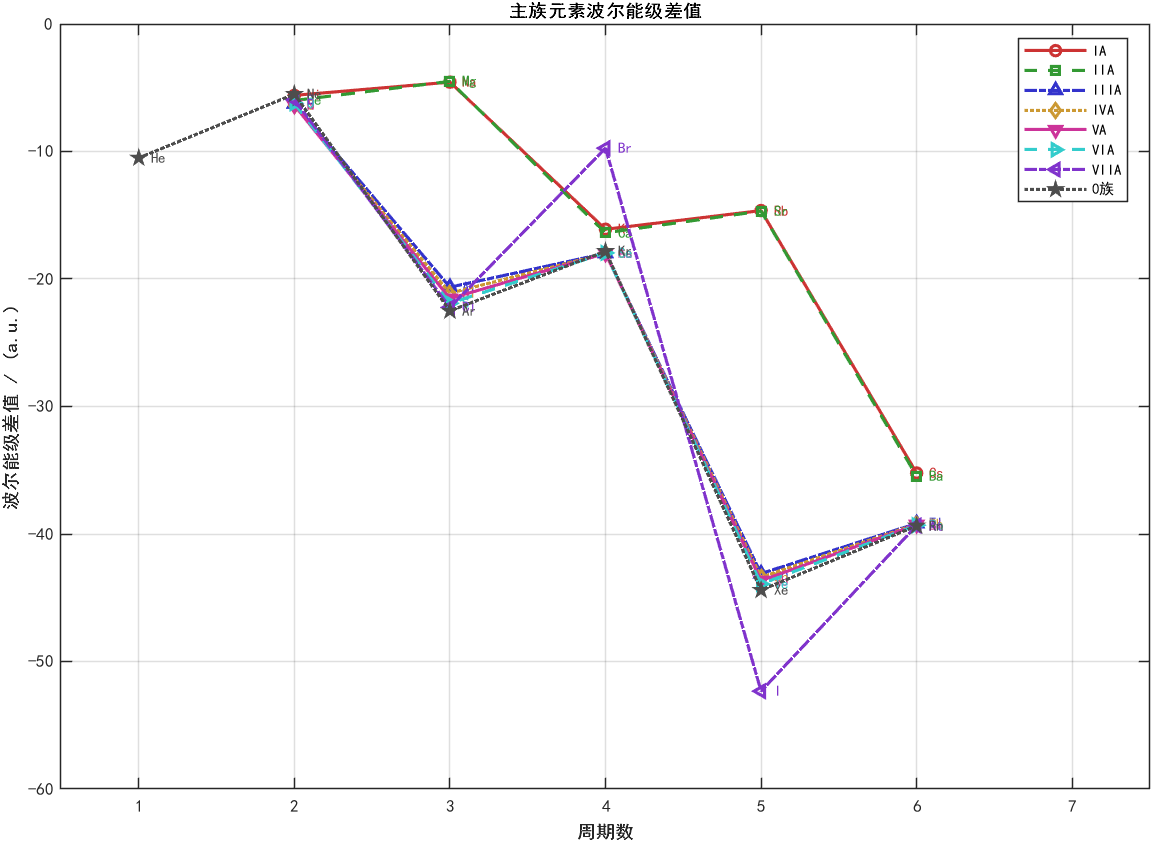
\includegraphics[width=\linewidth]{abol.png}
        \caption{主族-玻尔能级}
    \end{subfigure}\hfill
    \begin{subfigure}[t]{0.47\textwidth}
        \centering
        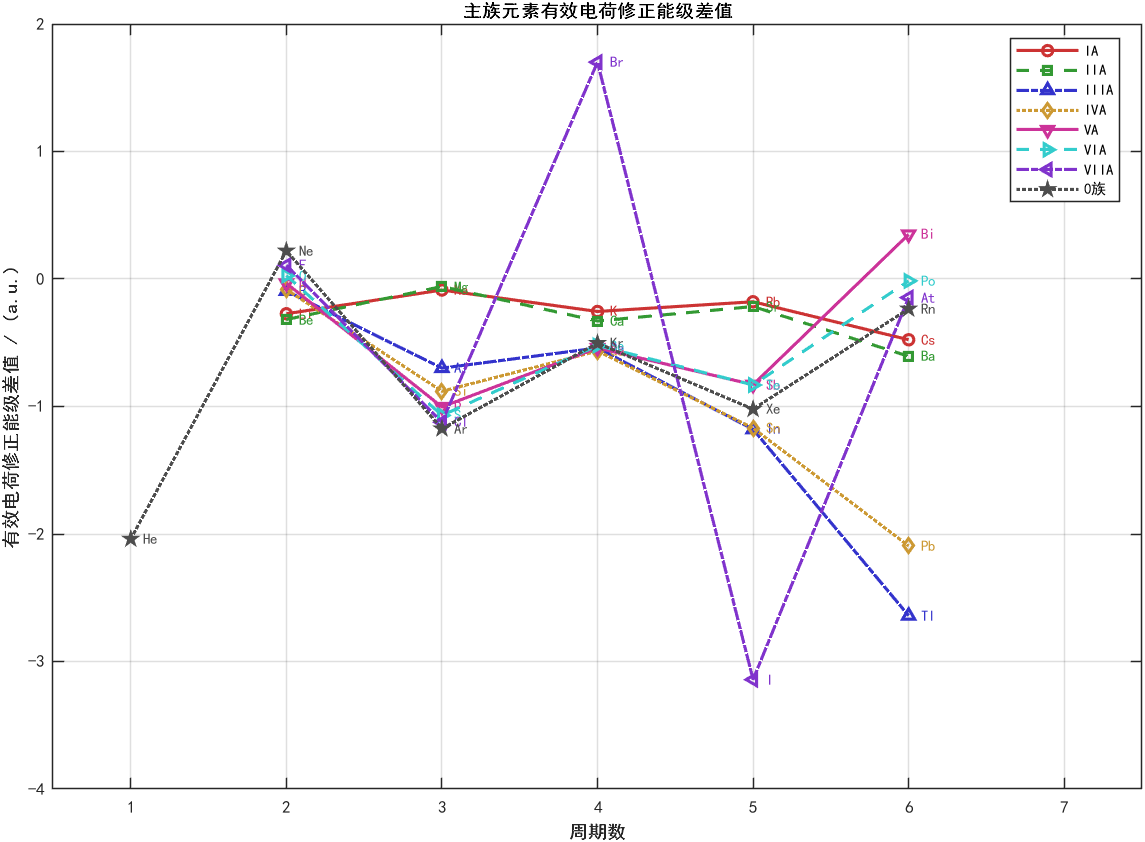
\includegraphics[width=\linewidth]{asch.png}
        \caption{主族-有效电荷修正}
    \end{subfigure}

    \vspace{0.3cm}

    \begin{subfigure}[t]{0.47\textwidth}
        \centering
        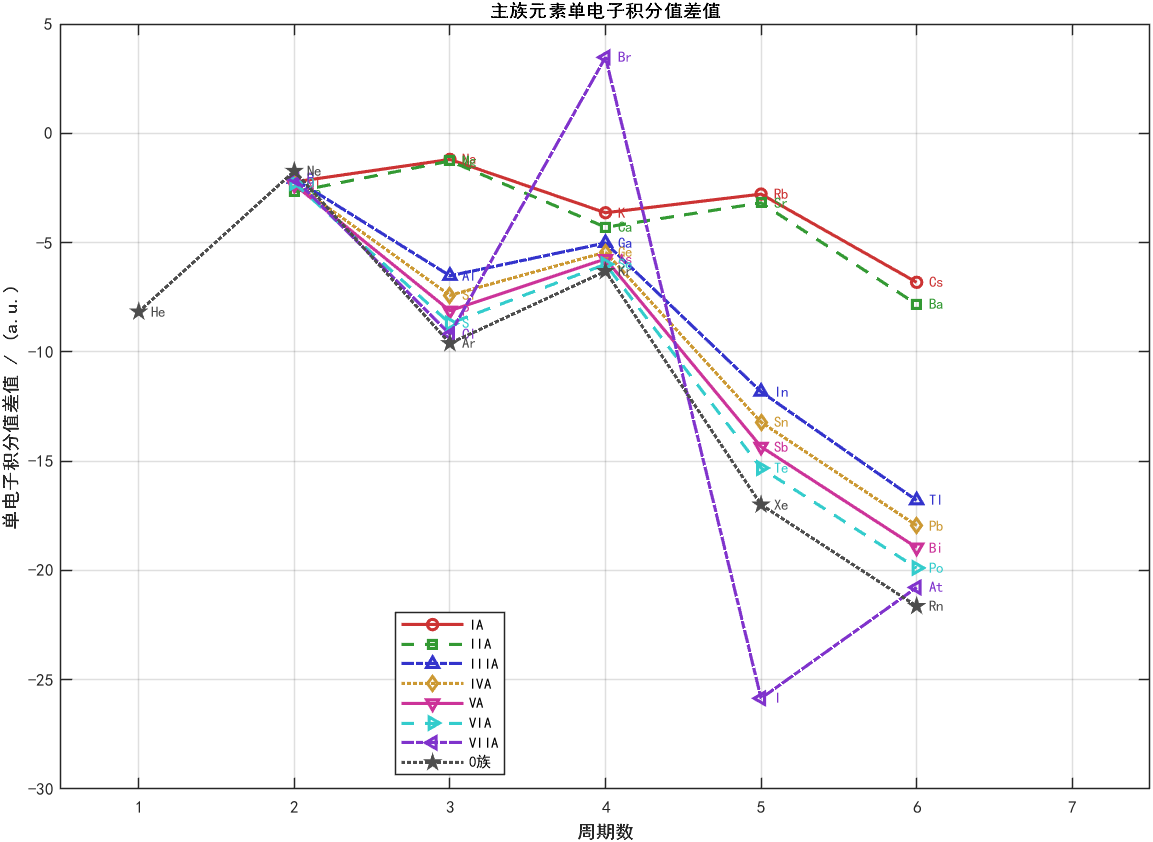
\includegraphics[width=\linewidth]{anon.png}
        \caption{主族-单电子积分}
    \end{subfigure}\hfill
    \begin{subfigure}[t]{0.47\textwidth}
        \centering
        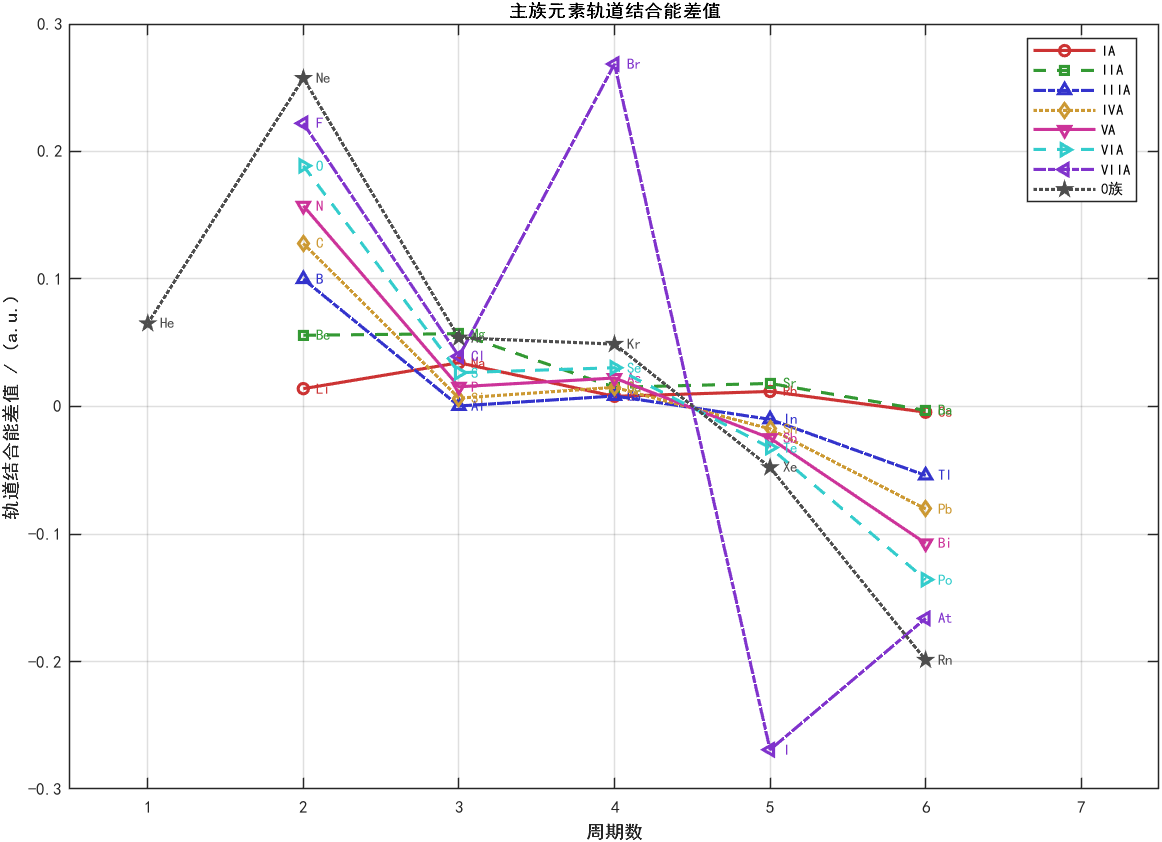
\includegraphics[width=\linewidth]{arel.png}
        \caption{主族-轨道结合能}
    \end{subfigure}
    \caption{主族数据对比图}
    \label{fig:main-group-compare}
\end{figure}


图~\ref{fig:main-group-compare} 给出了主族元素的玻尔能级，有效电荷修正的玻尔能级，单电子积分，轨道结合能的差值折线图。结果显示，玻尔能级普遍呈现显著的松紧数值特征，并在$s/p$区表现出不同模式：$s$区总体呈“大—小—大—小—大”，$p$区总体呈“小—大—小—大—小”，与已有研究描述基本一致。

对于$p$区元素，在纳入电子间相互作用后，第3、4主族元素的第4--6周期差值开始递减；考虑相对论效应后，$p$区元素除了第7主族，第4--6周期差值都呈现为递减态势；而在相对论效应基础上进一步引入电子相互作用修正后，保持与只引入相对论效应相同的特征。提示该区间可能存在由相对论效应主导的补偿效应。

对于零族元素，电子相互作用修正后保持松紧模式；引入相对论效应后，第4--6周期差值均呈递减趋势；而共同考虑相对论效应和电子相互作用修正后则呈现2--6周期单调减小的特征。说明封闭壳层体系中松紧效应的外显形式对相对论修正更敏感。


\begin{figure}[H]
    \centering
    \begin{subfigure}[t]{0.47\textwidth}
        \centering
        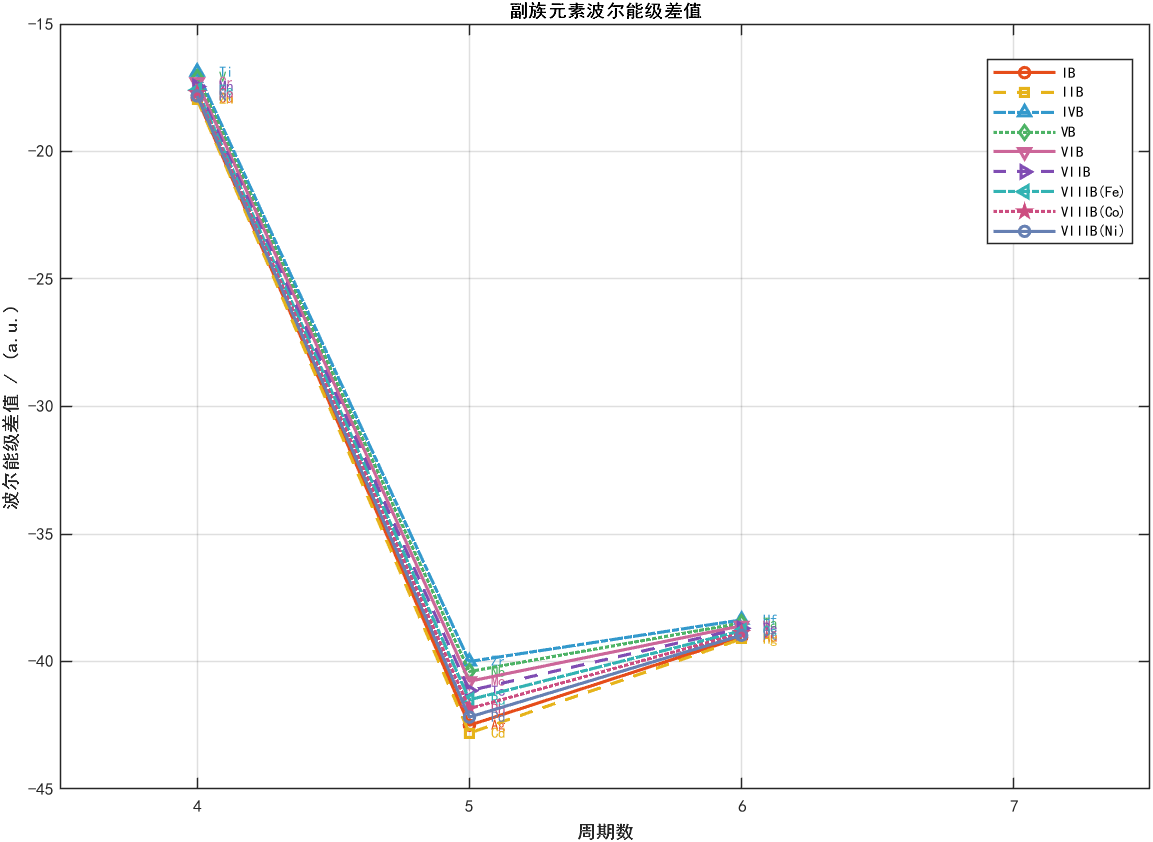
\includegraphics[width=\linewidth]{bbol.png}
        \caption{副族-玻尔能级}
    \end{subfigure}\hfill
    \begin{subfigure}[t]{0.47\textwidth}
        \centering
        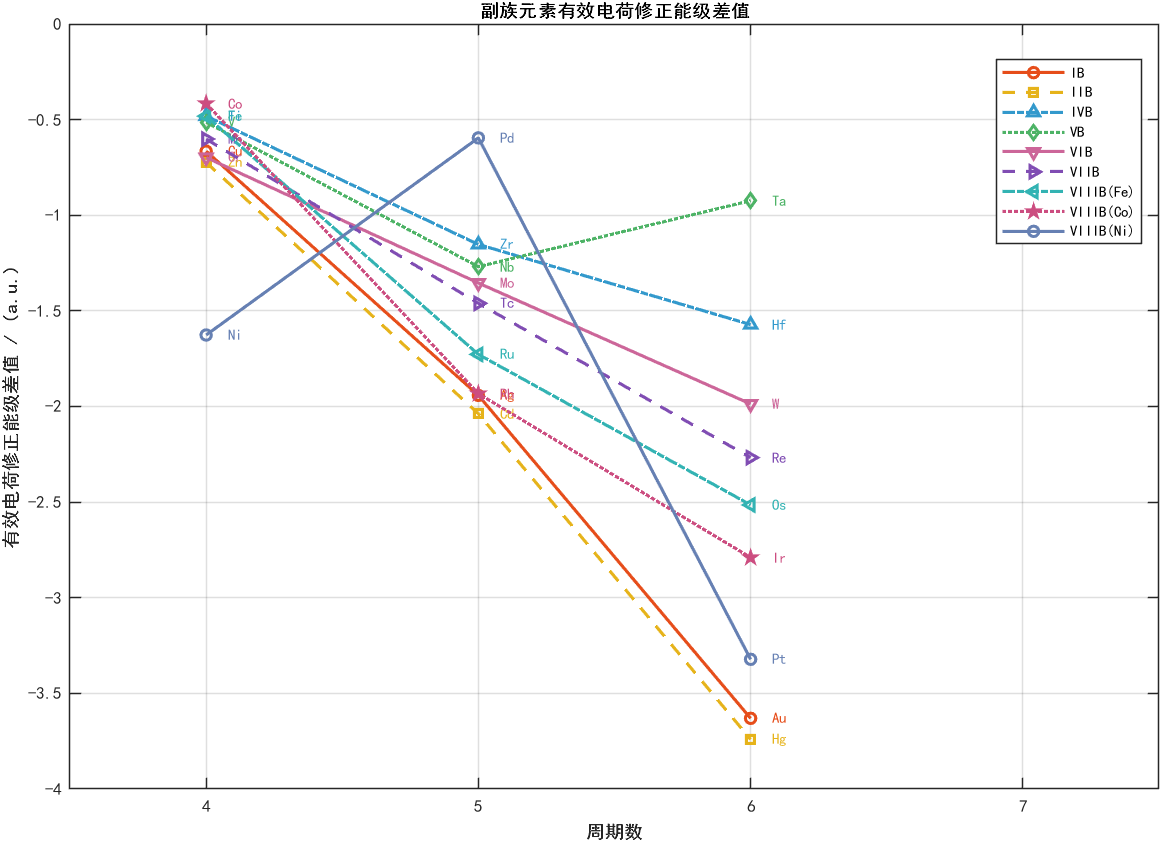
\includegraphics[width=\linewidth]{bsch.png}
        \caption{副族-有效电荷修正}
    \end{subfigure}

    \vspace{0.3cm}

    \begin{subfigure}[t]{0.47\textwidth}
        \centering
        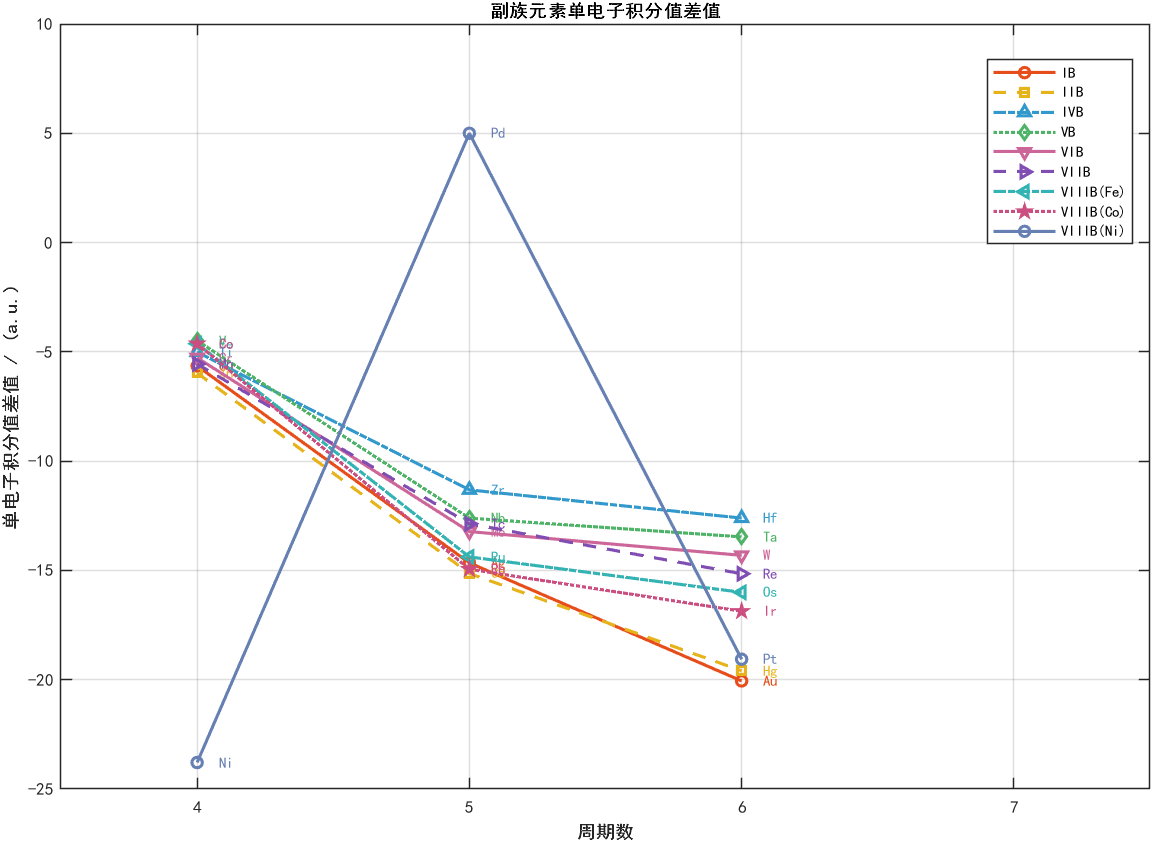
\includegraphics[width=\linewidth]{bnon.png}
        \caption{副族-单电子积分}
    \end{subfigure}\hfill
    \begin{subfigure}[t]{0.47\textwidth}
        \centering
        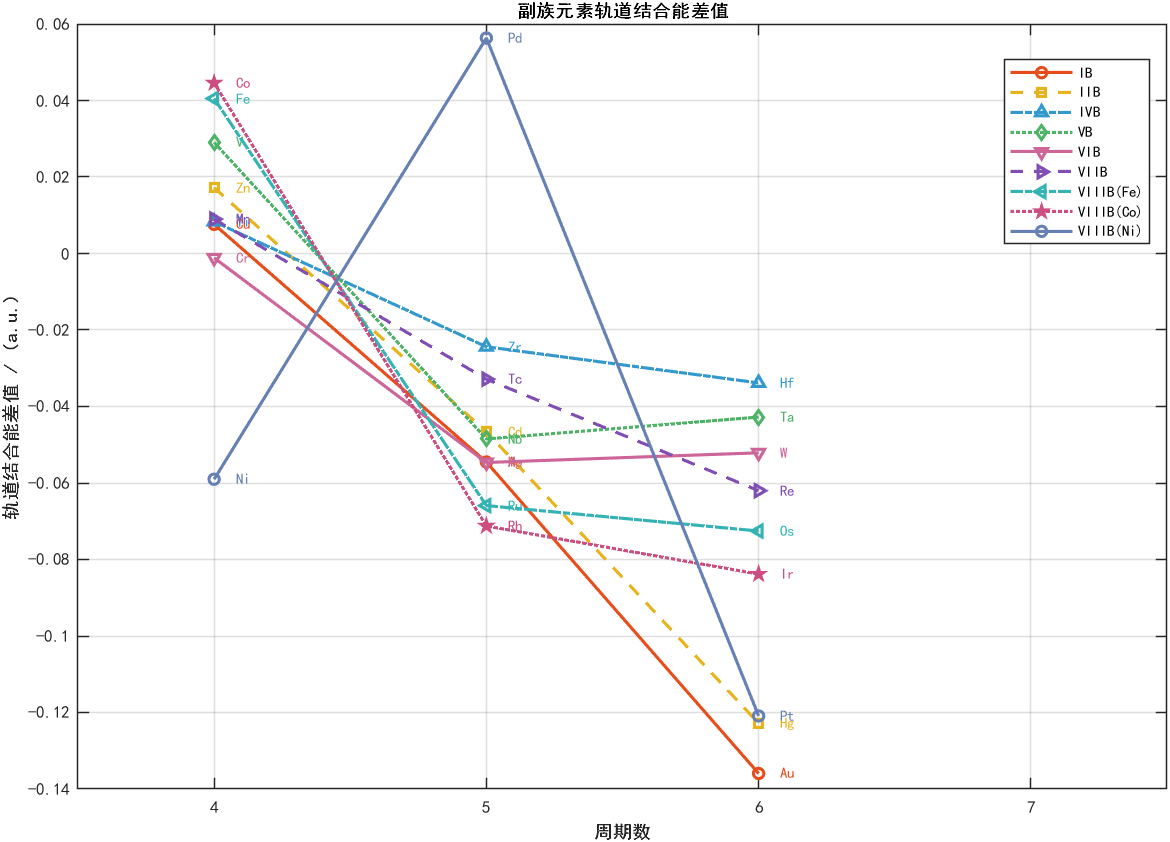
\includegraphics[width=\linewidth]{brel.png}
        \caption{副族-轨道结合能}
    \end{subfigure}
    \caption{副族数据对比图}
    \label{fig:subgroup-compare}
\end{figure}

图~\ref{fig:subgroup-compare} 给出了副族元素在不同计算方法下的差值折线图。对于副族元素，除第十副族及数据点不足的第三副族外，玻尔能级整体仍表现“小—大—小”特征。考虑电子相互作用后，除了第5、10副族外其余副族对应差值转为单调减小；考虑相对论效应后，除去第10副族其余副族全部出现同类趋势。而在电子相互作用修正下进一步引入相对论效应后，第5、6副族再次呈现松紧数值特征，表明在该区间电子相互作用与相对论效应之间存在一定程度的相互抵消。特别的，第十副族修正后全程呈现出“大-小-大”的松紧模式，暗示该族元素周期行为可能与$s$区元素呈现出相似特征

为从解析层面刻画“松紧效应”，考虑氢样能级表达式（见式（\ref{eq:bohr_zeff}））。
定义相邻周期对应的能级差为
\begin{equation}
\Delta E_n = E_{n+1}(Z+\Delta Z_n) - E_n(Z),
\end{equation}
其中 $\Delta Z_n$ 表示从第 $n$ 层填充至第 $n+1$ 层所需增加的核电荷数。根据电子层容量规则，有
\begin{equation}
\Delta Z_n \approx 2n^2.
\end{equation}

将其代入能级表达式，得
\begin{equation}
\Delta E_n = -\frac{(Z+\Delta Z_n)^2}{2(n+1)^2} + \frac{Z^2}{2n^2}.
\end{equation}

对 $\Delta Z_n$ 进行展开，并保留主导项，有
\begin{equation}
(Z+\Delta Z_n)^2 = Z^2 + 2Z\Delta Z_n + (\Delta Z_n)^2.
\end{equation}

代入后整理得
\begin{equation}
\Delta E_n \approx \frac{Z^2}{2}\left(\frac{1}{n^2} - \frac{1}{(n+1)^2}\right)
- \frac{Z\Delta Z_n}{(n+1)^2}
- \frac{(\Delta Z_n)^2}{2(n+1)^2}.
\end{equation}

注意到三项分别表现出不同的标度行为：
\begin{align}
\text{(i)}\;& \sim \frac{Z^2}{n^3}, \\
\text{(ii)}\;& \sim \frac{Z\,\Delta Z_n}{n^2} \sim Z, \\
\text{(iii)}\;& \sim \frac{(\Delta Z_n)^2}{n^2} \sim n^2.
\end{align}

由于 $\Delta Z_n \sim 2n^2$ 呈超线性增长，而 $n$ 仅线性递增，导致上述各项在不同周期区间的主导性发生交替变化：在低 $n$ 区域，第一项占主导，使 $\Delta E_n$ 较大；随着 $n$ 增大，第二、三项迅速增强并产生部分抵消，使 $\Delta E_n$ 减小；进一步增大 $n$ 时，高阶项再次占优，导致差值重新增大。

因此，$\Delta E_n$ 随周期变化会自然呈现“松—紧—松”的振荡结构。其首要来源不是额外修正项，而是 $Z$ 与 $n$ 在填充过程中的非对称增长；电子相互作用与相对论效应更多是在调节这一基本模式的幅度与适用边界。

从本文数据看，松紧效应在 \(s\) 区最稳定，\(p\) 区在第五周期后明显减弱，副族整体较弱，但第五、第六副族仍保留一定规律性。这说明：当电子填充基本遵循主量子层顺序时，结构性不对称更容易显现；而当 \(d\)、\(f\) 电子介入后，填充顺序的复杂化会削弱这一趋势。

这一结论既界定了松紧效应的适用范围，也为元素周期律教学提供了更清晰的边界参照，有助于学生区分“基本数学骨架”与“精细物理修正”各自的作用。
在无机化学教学中，建议采用“先骨架、后血肉”的教学路径：先引导学生从玻尔模型出发，理解$Z$与$n$的数学关系如何自然导致能级差的“松紧”振荡，进而建立起“数理必然性”的初步认识；随后再引入屏蔽效应与相对论效应，探讨其如何对基础模式进行修正与完善，从而解释各分区元素的具体反常。这种层次清晰、逻辑递进的讲解方式，不仅能辅助学生构建完整的知识体系，还能有效提升学生对化学规律本质的科学认知。
\newpage


% ===== [源文件缺失 ch2_2：2.1.2 起，源缺失（编译 PDF 存于 out/ch2_2/chapter.pdf）] =====

% ===== [源文件缺失 ch2_3：2.2 S区元素] =====

% ===== [源文件缺失 ch2_4：源缺失] =====

% ===== [源文件缺失 ch2_5：源缺失] =====

% ===== [源文件缺失 ch2_6：源缺失] =====

% ---- chunk ch2_7 : 2.x 具体元素（P区） ----


\subsection{具体元素}

\subsubsection{硼族元素}

硼族元素多成三个单键，因而总有一个$p$轨道是空的，从而常常伴有强缺电子性，作为$p$区元素，惰电子对效应，族首元素效应占有较大的影响。

\textbf{硼族元素（B, Al, Ga, In, Tl）部分物性参数}

\medskip
\renewcommand{\arraystretch}{1.2}
\noindent\begin{tabular*}{\textwidth}{@{\extracolsep{\fill}}lccccc@{}}
\toprule
性质 & B & Al & Ga & In & Tl \\
\midrule
共价半径/pm & 80 & 125 & 125 & 150 & 155 \\
金属半径/pm & -- & 143 & 141 & 166 & 171 \\
离子半径/pm & 27 & 53 & 62 & 80 & 89 \\
熔点/\(^{\circ}\mathrm{C}\) & 2300 & 660 & 30 & 157 & 304 \\
沸点/\(^{\circ}\mathrm{C}\) & 3930 & 2470 & 2403 & 2000 & 1460 \\
1$^{\mathrm{st}}$ 电离能/\(\mathrm{kJ\cdot mol^{-1}}\) & 799 & 577 & 577 & 556 & 590 \\
2$^{\mathrm{nd}}$ 电离能/\(\mathrm{kJ\cdot mol^{-1}}\) & 2427 & 1817 & 1979 & 1821 & 1971 \\
Pauling 电负性 & 2.0 & 1.6 & 1.8 & 1.8 & 2.0 \\
\(E^{\circ}(\mathrm{M^{3+}/M})/\mathrm{V}\) & -0.89 & -1.68 & -0.53 & -0.34 & +0.72 \\
\bottomrule
\end{tabular*}
\renewcommand{\arraystretch}{1.0}

硼族中族首元素 B 具有明显的“首元素效应”：原子半径小、电离能高、可用价层轨道较少，因此常表现出较低配位数与较强共价成键倾向。硼原子价层仅有 3 个价电子，典型三卤化硼（如 $\mathrm{BF_3}$、$\mathrm{BCl_3}$）属于缺电子 Lewis 酸，易与含孤对电子物种发生配位。其水解可生成硼酸（常写作 $\mathrm{B(OH)_3}$），体现出硼中心对电子对受体行为。另一方面，硼族缺电子中心常通过反馈 $\pi$ 相互作用（$p\pi$--$p\pi$）部分缓解电子不足，这也是解释其键长、键能与反应活性差异的重要观点。

从标准电极电势看，$\mathrm{Al^{3+}/Al}$ 为 $-1.68\ \mathrm{V}$（强还原性），而 $\mathrm{Tl^{3+}/Tl}$ 高达 $+0.72\ \mathrm{V}$（氧化性显著增强），这一跨度反映出重硼族元素中 $ns^2$ 惰性电子对效应的增强。所谓惰性电子对效应，是指随着族中原子序数增加，外层 $ns^2$ 电子对因相对论效应收缩且能级降低，越来越不愿参与成键或氧化。因此从 Ga 到 In 再到 Tl，$+3$ 氧化态的氧化性逐渐增强、稳定性下降，而 $+1$ 氧化态趋于稳定。事实上，Tl 在水溶液中主要以 $\mathrm{Tl^+}$ 形式存在，其化学行为更接近碱金属离子而非典型的 $+3$ 价硼族元素。

特别的，镓在结构和物性上具有若干“反常”特征：其原子/金属半径与 Al 接近甚至局部呈收缩趋势（与屏蔽不完全相关）；固态 Ga 易形成具有方向性的弱共价网络并可视作含二聚单元特征$Ga_2$，因此熔点较低。镓的晶体结构是正交晶系，二聚体之间靠较弱的金属键和范德华力维系。熔化时主要破坏的是二聚体之间的弱作用力，因此熔点极低。一旦熔化，这些共价方向性被破坏，液态 Ga 变成典型的密堆积金属液体。
熔化后，体系逐步转为更典型的\textbf{金属性液体结构}，使其液态温区较宽。价态方面，受惰性电子对效应影响，重硼族元素低价态稳定性增强，这一规律在 Ga 之后更为显著。

\newpage
\subsubsection{碳族}

\textbf{第四主族元素（C, Si, Ge, Sn, Pb）电负性（Pauling 标度）}

\medskip
\renewcommand{\arraystretch}{1.2}
\noindent\begin{tabular*}{\textwidth}{@{\extracolsep{\fill}}lccccc@{}}
\toprule
元素 & C & Si & Ge & Sn & Pb \\
\midrule
Pauling 电负性 & 2.55 & 1.90 & 2.01 & 1.96 & 2.33 \\
\bottomrule
\end{tabular*}
\renewcommand{\arraystretch}{1.0}

第四主族元素电负性整体上并非简单单调变化，呈现出“先降—小幅回升—再降—显著回升”的松紧特征（$\mathrm{C > Ge > Sn > Si}$，且 $\mathrm{Pb}$ 出现反常升高）。其中 $\mathrm{C\to Si}$ 的下降最明显，$\mathrm{Si\to Ge}$ 略有回升，$\mathrm{Ge\to Sn}$ 再次小幅降低，而 $\mathrm{Sn\to Pb}$ 回升幅度较大。该非单调性与屏蔽效应、轨道能级变化及相对论效应共同相关。

对碳而言，作为族首元素，原子半径最小、价层轨道紧凑，常形成稳定的定向共价键（如 $\mathrm{sp^3}$、$\mathrm{sp^2}$、$\mathrm{sp}$ 杂化），故电负性显著高于同族其余元素。由 C 到 Si 时，主量子数增加导致价电子平均距离增大，核吸引相对减弱，电负性明显下降。

由 Si 到 Ge 的轻微回升可广泛被理解为过渡金属后段 $d$ 电子屏蔽不完全带来的有效核电荷补偿效应；到 Sn 时，原子进一步增大，价电子束缚再度减弱，电负性出现小幅回落。

到 Pb 阶段，受相对论效应影响，$6s$ 轨道收缩增强，惰性电子对效应更显著；同时价层能级结构变化使其在 Pauling 标度上表现出明显偏高值。这也是重碳族元素化学行为与中间同族元素出现差异的重要原因之一。

\begin{center}
  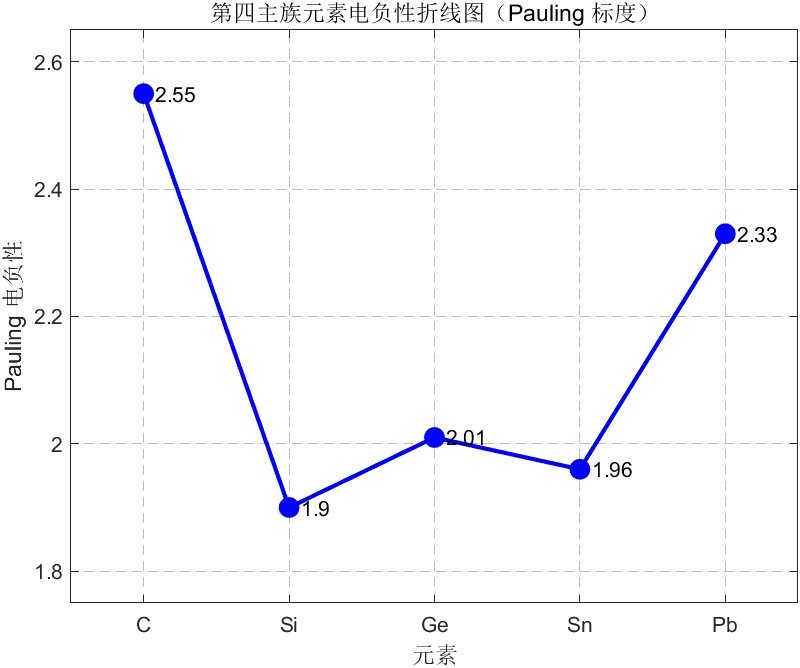
\includegraphics[width=0.5\textwidth]{CCC.png}
\end{center}

\newpage
\subsubsection{氮族}

\textbf{第五主族元素（N, P, As, Sb, Bi）电负性（Pauling 标度）}

\medskip
\renewcommand{\arraystretch}{1.2}
\noindent\begin{tabular*}{\textwidth}{@{\extracolsep{\fill}}lccccc@{}}
\toprule
元素 & N & P & As & Sb & Bi \\
\midrule
Pauling 电负性 & 3.04 & 2.19 & 2.18 & 2.05 & 2.02 \\
\bottomrule
\end{tabular*}
\renewcommand{\arraystretch}{1.0}

第五主族元素的电负性沿族总体呈下降趋势（$\mathrm{N > P \approx As > Sb > Bi}$），但相邻元素间降幅并不均匀，体现出一定的“松—紧”交替特征：$\mathrm{N\to P}$ 与 $\mathrm{As\to Sb}$ 的变化较明显，而 $\mathrm{P\to As}$ 与 $\mathrm{Sb\to Bi}$ 的变化较小。该非线性变化可用于辅助理解其氧化还原性质的阶段性差异。
\begin{center}
  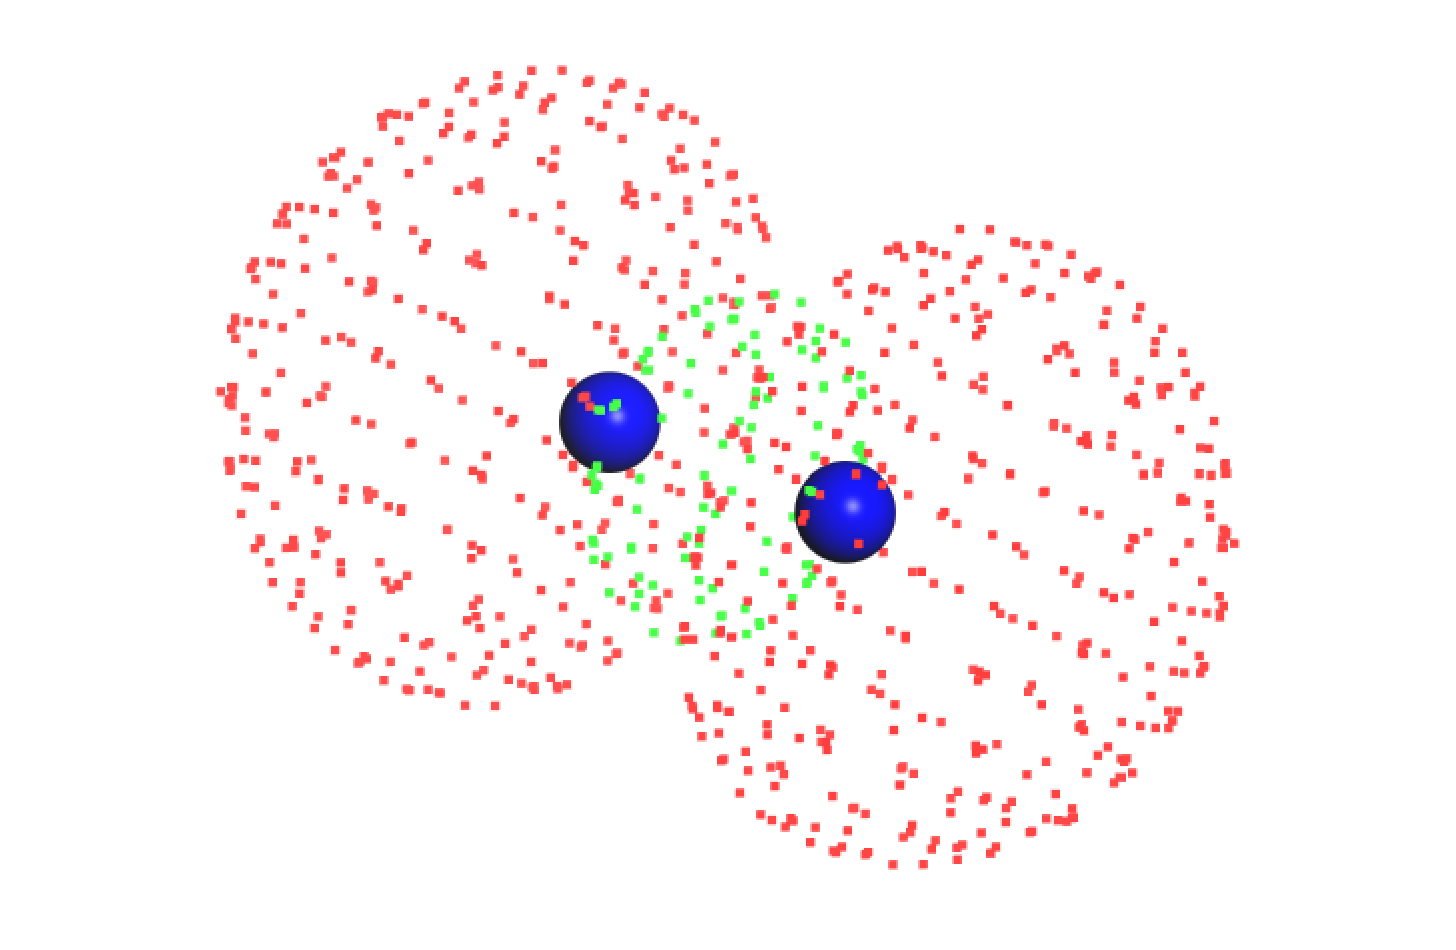
\includegraphics[width=0.5\textwidth]{N2HOMO.png}
\end{center}
对氮而言，作为族首元素，原子半径小、价层电子受核吸引较强，表现出明显“紧”的特征；但单质 $\mathrm{N_2}$ 由于三键键能高、动力学惰性强，其氧化还原行为需与分子稳定性区分讨论。氮的强氧化态特征更多体现在含氧含氮物种中。

磷相对更“松”，第二能层的紧使得有效核电荷数下降，第三能层价层电子束缚减弱，因此与氮相比更易参与成键重排；在常见化学环境下，磷的氧化性通常弱于对应高价氮物种，而还原性表现相对更突出。

由 P 到 As，受屏蔽效应变化与有效核电荷调整影响，电子束缚出现再增强趋势；同时随核电荷增大，相对论效应逐步显现，$s$ 轨道收缩与惰性电子对效应开始发挥作用。因此砷既可形成 +5 价物种（如砷酸盐体系），+3 价化合物的稳定性也明显提高。

到 Sb、Bi 阶段，相对论效应与惰性电子对效应进一步增强，+3 价通常比 +5 价更稳定；相应地，+5 价化合物整体氧化性更强、热力学稳定区间更窄。



\begin{center}
  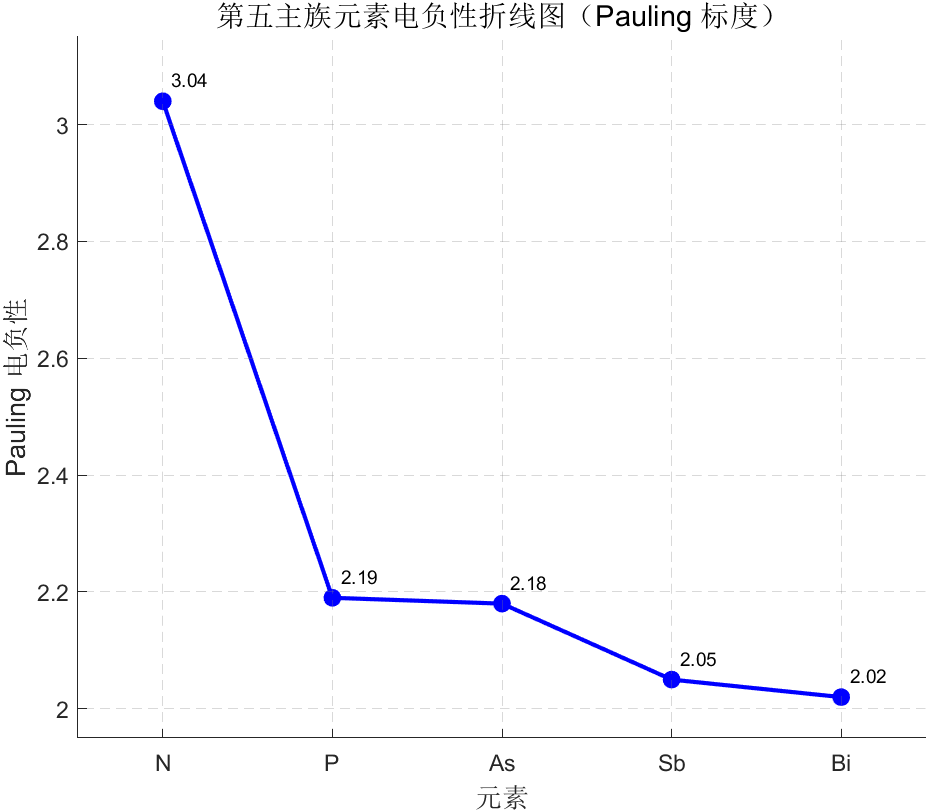
\includegraphics[width=0.5\textwidth]{NNN.png}
\end{center}


\newpage
\subsubsection{氧族}

\textbf{第六主族元素（O, S, Se, Te, Po）电负性（Pauling 标度）}

\medskip
\renewcommand{\arraystretch}{1.2}
\noindent\begin{tabular*}{\textwidth}{@{\extracolsep{\fill}}lccccc@{}}
\toprule
元素 & O & S & Se & Te & Po \\
\midrule
Pauling 电负性 & 3.44 & 2.58 & 2.55 & 2.10 & 2.00 \\
\bottomrule
\end{tabular*}
\renewcommand{\arraystretch}{1.0}

第六主族元素电负性沿族总体下降（$\mathrm{O > S \approx Se > Te > Po}$），但降幅并不均匀：$\mathrm{O\to S}$ 下降最显著，$\mathrm{S\to Se}$ 仅小幅变化，而到 $\mathrm{Te\to Po}$ 继续降低。该趋势体现了主量子数增加导致的价电子平均距离增大，以及屏蔽效应、相对论效应对重元素的共同影响。

氧作为族首元素，半径小、价层电子受核吸引强，电负性显著偏高，因此在含氧化合物中常表现出较强吸电子能力。由 O 到 S 时，价层从第二周期跃迁到第三周期，电子云显著外扩，电负性明显下降。

从 S 到 Se 变化较小，可理解为轨道扩展与有效核电荷补偿的共同结果；到 Te、Po 阶段，原子半径继续增大且重元素效应更复杂，整体仍表现为电负性降低。对应化学行为上，重氧族元素形成高氧化态物种的稳定区间通常收缩，低氧化态相对更常见。

\begin{center}
  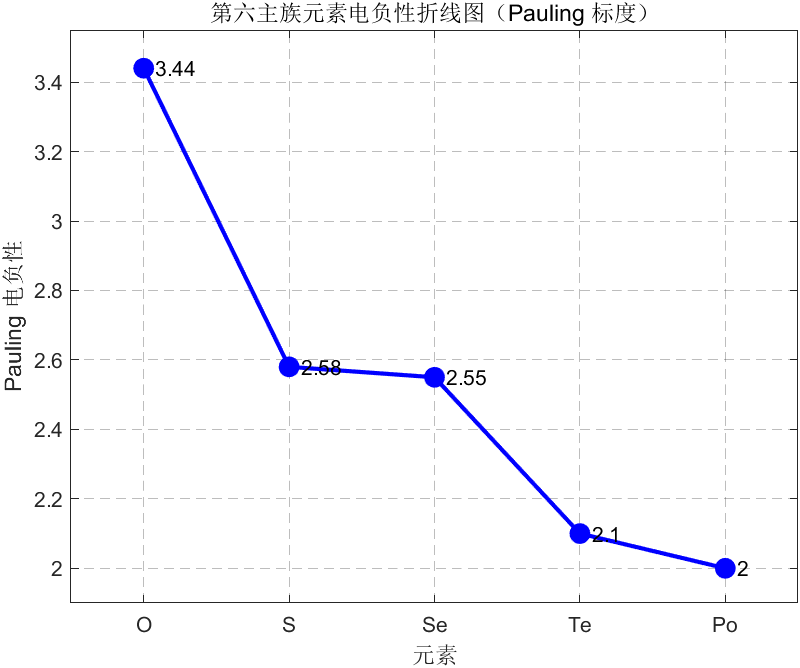
\includegraphics[width=0.5\textwidth]{OOO.png}
\end{center}





氧族元素有一个特殊的单质——臭氧。
臭氧 $\mathrm{O_3}$ 可由两条等价共振式表示（$\mathrm{O{=}O{-}O^-}$ 与 $\mathrm{^-O{-}O{=}O}$），其本质是三中心四电子（3c--4e）离域 $\pi$ 键：
\[
\mathrm{O_3:}\quad \text{两端 O--O 键级均约为 }1.5
\]
因此两条 O--O 键长度近似相等，分子呈弯曲结构并具有较强氧化性。

与之对比，硫的同素体化学更偏向形成单键环状结构（如 $\mathrm{S_8}$）。虽然 $\mathrm{S_3}$ 物种可在气相或瞬态条件下观测到，但常温常压下难以形成与臭氧对应的稳定“臭硫”分子。主要原因包括：
\begin{enumerate}
  \item $3p$ 轨道离域重叠效率低于氧的 $2p$ 体系，稳定离域 $\pi$ 键的能力较弱；
  \item 硫原子半径更大、键角与成键能匹配不利于臭氧式弯曲三原子结构长期稳定；
  \item 热力学上硫更倾向转化为多硫环/链结构而非维持三原子离域体系。
\end{enumerate}


\newpage
\subsubsection{氟族}

\textbf{第七主族元素（F, Cl, Br, I, At）电负性（Pauling 标度）}

\medskip
\renewcommand{\arraystretch}{1.2}
\noindent\begin{tabular*}{\textwidth}{@{\extracolsep{\fill}}lccccc@{}}
\toprule
元素 & F & Cl & Br & I & At \\
\midrule
Pauling 电负性 & 3.98 & 3.16 & 2.96 & 2.66 & 2.20 \\
\bottomrule
\end{tabular*}
\renewcommand{\arraystretch}{1.0}

第七主族（卤素）电负性沿族呈明显下降趋势（$\mathrm{F > Cl > Br > I > At}$），其中 $\mathrm{F\to Cl}$ 的降幅最大，之后逐步趋缓。该规律与卤素从强吸电子非金属向较弱吸电子重卤素过渡的化学行为一致。

氟的电负性在全部元素中最高，源于其极小原子半径与高有效核吸引；因此 F 在成键中最易夺取电子密度，且几乎不表现正氧化态。由 Cl、Br 到 I，随电子云外扩与屏蔽增强，电负性依次减小，氧化性总体减弱。

到 At 阶段，重元素相对论效应与轨道能级变化进一步增强，其电负性继续下降；对应地，化学行为较轻卤素更偏向“金属性增强、典型卤素性减弱”的方向。


\begin{center}
  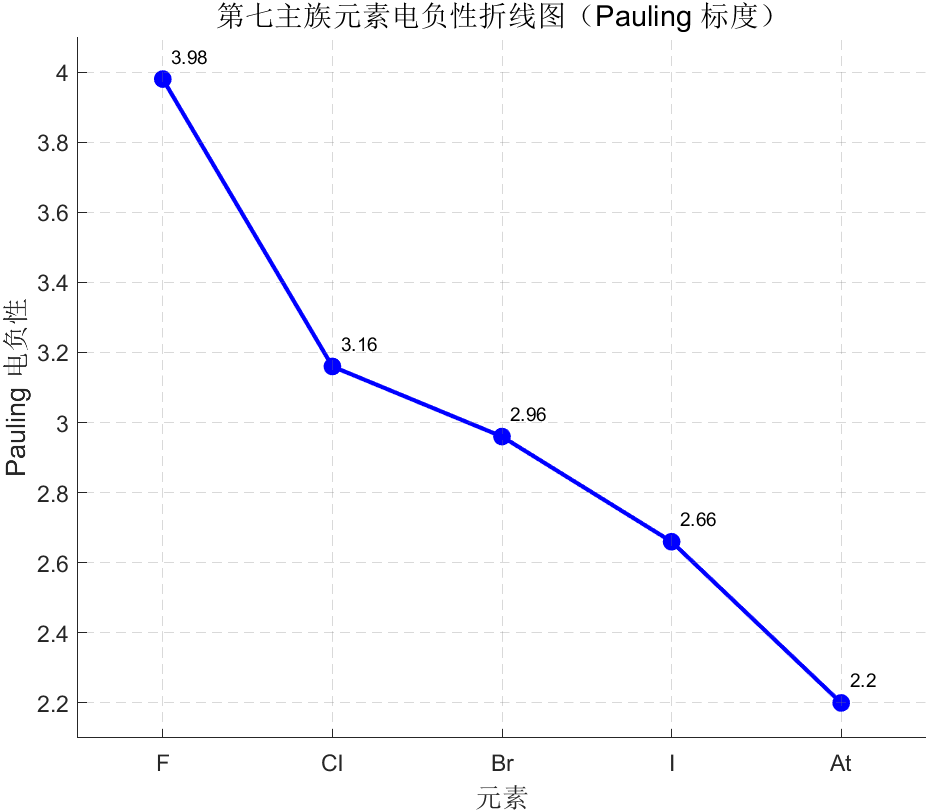
\includegraphics[width=0.5\textwidth]{FFF.png}
\end{center}

\textbf{卤素单质键能对比（$\mathrm{X_2}$，近似键解离能）}

\medskip
\renewcommand{\arraystretch}{1.2}
\noindent\begin{tabular*}{\textwidth}{@{\extracolsep{\fill}}lccccc@{}}
\toprule
分子 & $\mathrm{F_2}$ & $\mathrm{Cl_2}$ & $\mathrm{Br_2}$ & $\mathrm{I_2}$ & $\mathrm{At_2}$（估计） \\
\midrule
$D_0$ / $\mathrm{kJ\cdot mol^{-1}}$ & 158 & 243 & 193 & 151 & $\sim 110$--130 \\
\bottomrule
\end{tabular*}
\renewcommand{\arraystretch}{1.0}

从整体看，卤素单质键能并不单调下降：$\mathrm{Cl_2}$ 反而高于 $\mathrm{F_2}$，随后沿 $\mathrm{Cl_2\to Br_2\to I_2}$ 逐步降低。$\mathrm{F_2}$ 键能“反常偏低”的核心原因是：
\begin{enumerate}
  \item 氟原子半径极小，成键后两原子距离很短，非键电子对之间排斥显著增强；
  \item $2p$ 轨道重叠虽强，但短键距下电子-电子排斥对键稳定化的抵消更明显；
  \item 因而净成键稳定化不足以达到“最强 X--X 键”，导致 $\mathrm{F_2}$ 的 $D_0$ 低于 $\mathrm{Cl_2}$。
\end{enumerate}


现在我们来聊聊卤素和水之间的事情。你可能会想：氯气溶于水，不就是溶解吗？没那么简单。卤素和水之间发生的是一连串既有氧化还原、又有歧化、还受酸碱平衡牵制的复杂反应。更有趣的是，从氟到碘，每个卤素的“脾气”都不太一样。

我们先看氟。氟气是卤素里最凶猛的氧化剂，它跟水根本不谈什么可逆平衡——上来就把水氧化了，放出氧气，自己变成 HF。这个过程干脆利落，没有中间商赚差价。因为氟几乎不形成稳定正氧化态，所以它也不走什么“次氟酸”的路径，跟下面几个卤素完全是两条路。

往下走到氯和溴，情况就不同了。氯气和溴气溶于水时，会跟水达成一种可逆的歧化平衡：一个卤原子被氧化成 $+1$ 价（生成次卤酸 HXO），另一个被还原成 $-1$ 价（生成氢卤酸 HX）。写成反应式就是：
\[
\mathrm{X_2 + H_2O \rightleftharpoons HX + HXO}\quad (\mathrm{X=Cl,Br})
\]
这个平衡对 pH 非常敏感。你往溶液里加碱，HXO 被中和成 XO$^-$，平衡就被拉着向右跑；你加酸，反应就往回退。HOCl 和 HOBr 本身也是相当活性的氧化剂——漂白剂和消毒水的有效成分就是它们。

再往下到碘，平衡常数就很小了。碘在水里的溶解度本来就低，歧化也没那么情愿。不过碘有个巧妙的招数：它会拉着溶液里的碘离子（I$^-$）形成三碘离子 I$_3^-$，借助这个配合物的形成来提高表观溶解度。所以碘在水里的行为，既有氧化还原，又有配位化学参与进来。

总的趋势很明确：从氟到碘，氧化性越来越弱，和水反应的驱动力越来越小。但这不只是单一趋势——氟直接氧化水，氯和溴走可逆歧化平衡，碘则被溶解度和平衡常数双重拖累，每一步都体现了它们在周期表位置上的微妙差异。

\medskip

如果我们换个角度，不以单个卤素分子为出发点，而是以“中心卤素原子”的视角来看，事情还有另一层规律。卤素水解后生成的含氧物种——次卤酸根（XO$^-$）、亚卤酸根（XO$_2^-$）、卤酸根（XO$_3^-$）、高卤酸根（XO$_4^-$）——它们的形成趋势沿族有明显的递变。

氯是这条规律最“标准”的执行者。Cl$_2$ 在水中生成 HOCl/OCl$^-$，在碱性条件下加热，OCl$^-$ 还会进一步歧化成 Cl$^-$ 和 ClO$_3^-$。这条从 $0$ 到 $-1$ 和 $+1$，再从 $+1$ 到 $-1$ 和 $+5$ 的歧化链路，氯走得相当顺畅。

溴也走类似的路，但它的各种含氧酸根稳定区间都比氯窄一些。HOBr/OBr$^-$ 比次氯酸根更容易继续歧化或被还原掉，所以在溶液里维持高浓度比较困难。

碘的次碘酸 HOI 稳定性就更差了，几乎一生成就急着进一步歧化成 I$^-$ 和 IO$_3^-$。所以在碘的溶液化学中，碘酸根比次碘酸根常见得多。

氟呢，作为中心原子几乎不形成稳定的正氧化态，所以根本就没有这个“典型次卤酸平衡”的路径。你大可以把氟当作这条规律的例外来处理，记住它自成一家就好。

\medskip

把这些现象串起来，我们可以用一个“先水解、后歧化或重排”的模型来统一理解:
\begin{enumerate}
    \item 第一步，卤素分子和水作用，一个原子变成 $-1$ 价氢卤酸，另一个变成 $+1$ 价次卤酸。
    \item 第二步，次卤酸根 XO$^-$ 不会老老实实待着——它可以走歧化通道，同一个中间体既被氧化又被还原，生成卤离子和高价含氧卤离子；也可以走重排通道，通过氧原子迁移和键重组，向更稳定的含氧阴离子分布演化。
\end{enumerate}

具体走哪条路、停在哪个氧化态，取决于卤素的种类、溶液的 pH 和温度。整个图景并不复杂：就是氧化还原和歧化两条主线交织在一起，由一个酸碱平衡的天平在背后调控着。

\medskip

最后说说互卤素——就是不同卤素之间形成的化合物，比如 ICl、BrF$_3$、IF$_7$ 这类。它们水解的规律其实很直觉：两种卤素原子里，电负性弱的那个当“中心原子”，水解后变成含氧酸；电负性强的那个当“末端原子”，水解后变成氢卤酸。一条简单的近似规则是：
\[
\mathrm{XY + H_2O \rightarrow HOX + HY}
\]
X 是电负性较弱的中心原子，Y 是电负性较强的末端原子。拿 ICl 来说，I 的电负性比 Cl 小，所以 I 是中心原子，生成 HOI（次碘酸），Cl 是末端原子，生成 HCl。IBr 同理，I 是中心，生成 HOI 和 HBr。BrCl 里 Br 是中心，生成 HOBr 和 HCl。

如果中心原子本身已经带了较高的氧化态，那么水解就会直接生成对应的更高价含氧酸。比如 ClF$_3$ 水解，Cl 是 $+3$ 价中心原子，就生成亚氯酸 HClO$_2$ 和 HF：
\[
\mathrm{ClF_3 + 2H_2O \rightarrow HClO_2 + 3HF}
\]
BrF$_3$ 也一样，生成亚溴酸和 HF。

IF$_5$ 水解，I 是 $+5$ 价，就直接生成碘酸 HIO$_3$：
\[
\mathrm{IF_5 + 3H_2O \rightarrow HIO_3 + 5HF}
\]
IF$_7$ 更是把 I 顶到了 $+7$ 价，水解给出高碘酸 HIO$_4$：
\[
\mathrm{IF_7 + 4H_2O \rightarrow HIO_4 + 7HF}
\]

你看，互卤素水解的规则根本不用死记：找出谁的电负性小，它就是中心原子，变成含氧酸；电负性大的变成氢卤酸。中心原子的氧化态有多高，含氧酸的氧化态就有多高，水分子数目自然配平。整个逻辑链条是透明的，从电负性大小直接就能推出来。

\newpage
\subsubsection{稀有气体}

现在我们来谈谈稀有气体——周期表最右边那一列，曾经被叫做“惰性气体”。这个名字起得不太好，因为它暗示这些家伙什么都不肯干。实际上，从氪往下，稀有气体是可以参与化学反应的，而且它们的化合物还相当有趣。

稀有气体（He、Ne、Ar、Kr、Xe、Rn）最外层电子排布通常为闭壳层，因此单原子稳定、第一电离能较高、电子亲和倾向弱，常温下多以单原子分子形式存在。沿族向下，原子半径增大、极化率增大、电离能降低，因此从 He 到 Xe/Rn，参与成键的可能性逐渐增强。

\textbf{稀有气体第一电离能数据（单位：$\mathrm{kJ\cdot mol^{-1}}$）}

\medskip
\renewcommand{\arraystretch}{1.15}
\noindent\begin{tabular*}{\textwidth}{@{\extracolsep{\fill}}lcccccc@{}}
\toprule
元素 & He & Ne & Ar & Kr & Xe & Rn \\
\midrule
第一电离能 & 2372 & 2081 & 1521 & 1351 & 1170 & 1037 \\
\bottomrule
\end{tabular*}
\renewcommand{\arraystretch}{1.0}

从表中可见，稀有气体第一电离能沿族整体\textbf{单调下降}。这说明从 He 到 Rn，最外层电子受原子核束缚逐渐减弱，因此较重稀有气体更容易被极强化学条件活化，其中 Xe、Kr 最容易形成已知稳定化合物。


\begin{center}
  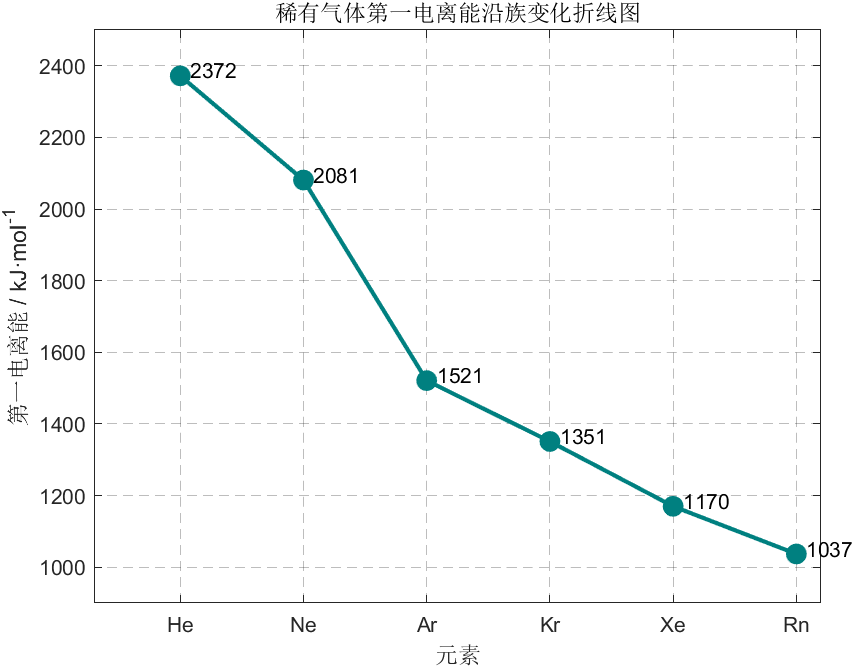
\includegraphics[width=0.8\textwidth]{HeHeHe.png}
\end{center}



我们先从最基本的物理性质说起。稀有气体都是无色无味的气体，沸点和熔点低得可怜——这很好理解，它们以单原子分子存在，彼此之间只有微弱的色散力在起作用。色散力虽然弱，但随着原子半径增大、电子云越来越“软”、越来越容易极化，这种吸引力也会逐渐增强。所以从氦到氡，沸点是逐步升高的。

接下来是关键问题：为什么稀有气体这么“懒”？答案就写在它们的电子结构上。价层全满——对轻稀有气体来说，这意味着无论是再塞一个电子进去，还是从里面拽一个电子出来，能量上都非常不划算。所以氦、氖、氩在通常条件下几乎不参与任何化学反应，它们是真正的“社交绝缘体”。

但事情到了氪和氙就开始起变化了。它们的原子半径大得多，最外层电子离核更远，束缚得没那么紧。这就意味着，如果碰上一个足够强的氧化剂、一个足够贪恋电子的配体——比如氟和氧——氪和氙的外层电子是可以被拉出来参与成键的。换句话说，不是稀有气体不反应，是你没找对反应对象。一旦氟这样的“电子强盗”出场，氙就乖乖就范，形成一系列相当稳定的氟化物和氧化物。

那么，稀有气体要成键，需要满足什么条件？经验上大概有三条。
\begin{itemize}
  \item 第一，得有个高电负性的配体来当搭档，氟和氧是最佳人选——它们能把中心原子的电子云拽过来，把高氧化态稳定住。
  \item 第二，反应条件得够劲——直接氟化、放电、紫外光照或者高压，总之得给体系注入足够的能量让稀有气体从全满的舒适区里走出来。
  \item 第三，中心原子得足够大、足够“软”，电子云能灵活地重新排布，以容纳成键带来的剧烈变化。
\end{itemize}

这就是为什么氙的化合物最多、最稳定，氪次之，氡虽然有潜力但自己先衰变了，化学研究很有限。

目前已知的典型稀有气体化合物包括：
\[
\mathrm{XeF_2,\; XeF_4,\; XeF_6,\; XeO_3,\; XeO_4,\; KrF_2}
\]
其中氙是绝对的明星，它的氟化物和氧化物构成了稀有气体化学的主体。

\medskip

好的，现在我们来处理一个更深的问题：$\mathrm{XeF_2}$ 是怎么成键的？按传统的八隅体规则，氙已经是满壳层了，凭什么再跟两个氟原子结合？你当然可以说这叫“超价”——氙的价电子超过了八个。但这个说法只是给现象贴了个标签，并没有解释清楚电子到底是怎么排的。

真正有意思的图景来自分子轨道理论。以线形的 $\mathrm{F\!-\!Xe\!-\!F}$ 为例，我们只关注沿着键轴方向的那个“骨架”：两个末端氟原子各出一个 $p$ 轨道，中心的氙也出一个对应的轨道。三个原子轨道组合在一起，会形成三个分子轨道——一个成键的、一个近似非键的、一个反键的。现在来数电子：两个氟各提供一个电子，氙在这个方向上贡献什么呢？可以认为氙拿出一对原来属于自己的电子放进这个三原子轨道体系。总共是四个电子，刚好填满成键轨道和非键轨道，反键轨道空着。

这就是著名的\textbf{三中心四电子键}（3c--4e 键）。写成填充方式就是：
\[
\sigma_{\text{成键}}^2\; \sigma_{\text{非键}}^2\; \sigma_{\text{反键}}^0
\]
四个电子分配到三个原子上，意味着两个 Xe--F 键的键级各自只有大约 $0.5$——比普通的单键弱。电子也不是定域在某一个 Xe--F 对上，而是离域在整个 F--Xe--F 三原子骨架之间。这就很自然地解释了为什么 $\mathrm{XeF_2}$ 是线形的，为什么它的 Xe--F 键比普通共价单键长，为什么它比较容易断裂。

这个三中心四电子键模型不只适用于 $\mathrm{XeF_2}$，也同样适用于 $\mathrm{KrF_2}$、三碘离子 $\mathrm{I_3^-}$ 以及其他看起来“电子超标”的线形体系。它的核心思想是：不要老想着中心原子硬塞了超过八个电子，而是要把电子看成分布在整个分子骨架上的离域波函——所谓的“超价”其实是一个离域成键问题，不是八隅体的机械扩充。

\medskip

如果你更喜欢用 VSEPR 的方式来直观理解，也没问题。拿 $\mathrm{XeF_2}$ 来说，氙周围有两对成键电子（连着两个氟）和三对孤对电子，总共五对电子域。五对电子域在空间里按三角双锥排布。关键来了：孤对电子之间排斥最厉害，它们一定要占据赤道平面上的三个位置，离得最远，彼此夹角 $120^\circ$。成键电子对就被挤到上下两个轴向顶点，形成一条直线——结果就是线形的 F--Xe--F，键角 $180^\circ$，和实验完全吻合。

用同样的逻辑推下去：$\mathrm{XeF_4}$ 是六对电子域——四个成键对加两个孤对——排成正八面体。两对孤对占据相对的两个顶点，剩下四个氟在赤道平面上排成一个正方形，所以分子是正方平面构型。$\mathrm{XeF_6}$ 更复杂些，六对成键加一对孤对，电子域排布本身就不那么对称，导致分子结构偏离完美的八面体，常呈现畸变八面体甚至单帽八面体的特征。

你看，无论是用分子轨道去追踪电子到底填在哪些轨道里，还是用 VSEPR 去画电子对互斥排布，两种思路指向的是同一个物理事实。VSEPR 给你直观的空间图像，三中心四电子键给你电子离域的定量说明——两者配合起来，稀有气体化合物的结构和成键就变得通透而自然。

\medskip

最后总结几句。稀有气体不是绝对不反应的——轻的（He、Ne、Ar）确实极难成键，但重的（Kr、Xe、Rn）在合适条件下可以和强电负性配体形成稳定化合物。氙是这个家族里最活跃的成员，它的氟化物和氧化物构成了稀有气体化学的主要版图。三中心四电子键是理解 $\mathrm{XeF_2}$、$\mathrm{KrF_2}$、$\mathrm{I_3^-}$ 这类线形超价分子的关键工具——它告诉我们，电子不足的稳定结构不是靠中心原子打破八隅体硬撑，而是靠电子在多原子骨架上离域来实现的。“超价”这个词，与其理解成“价电子超过八个”，不如理解成“成键电子分布在超过两个原子之间”。

\newpage


% ---- chunk ch2_8 : 2.x 碱金属/碱土后续 ----


\subsection{氧化物}

\subsubsection{含氮氧化物}
\begin{figure}[htbp]
    \centering
    \begin{subfigure}[b]{0.3\textwidth}
        \centering
        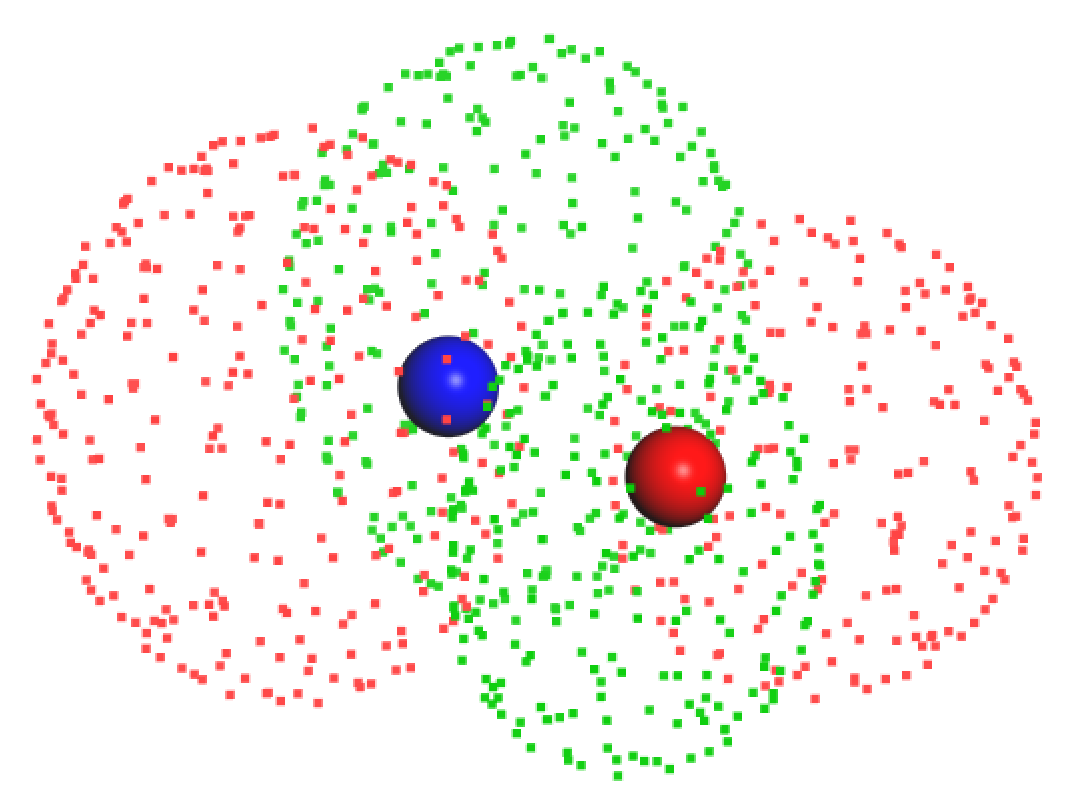
\includegraphics[width=\textwidth]{NOHOMO.png}
        \caption{NO HOMO}
        \label{fig:no}
    \end{subfigure}
    \hfill
    \begin{subfigure}[b]{0.3\textwidth}
        \centering
        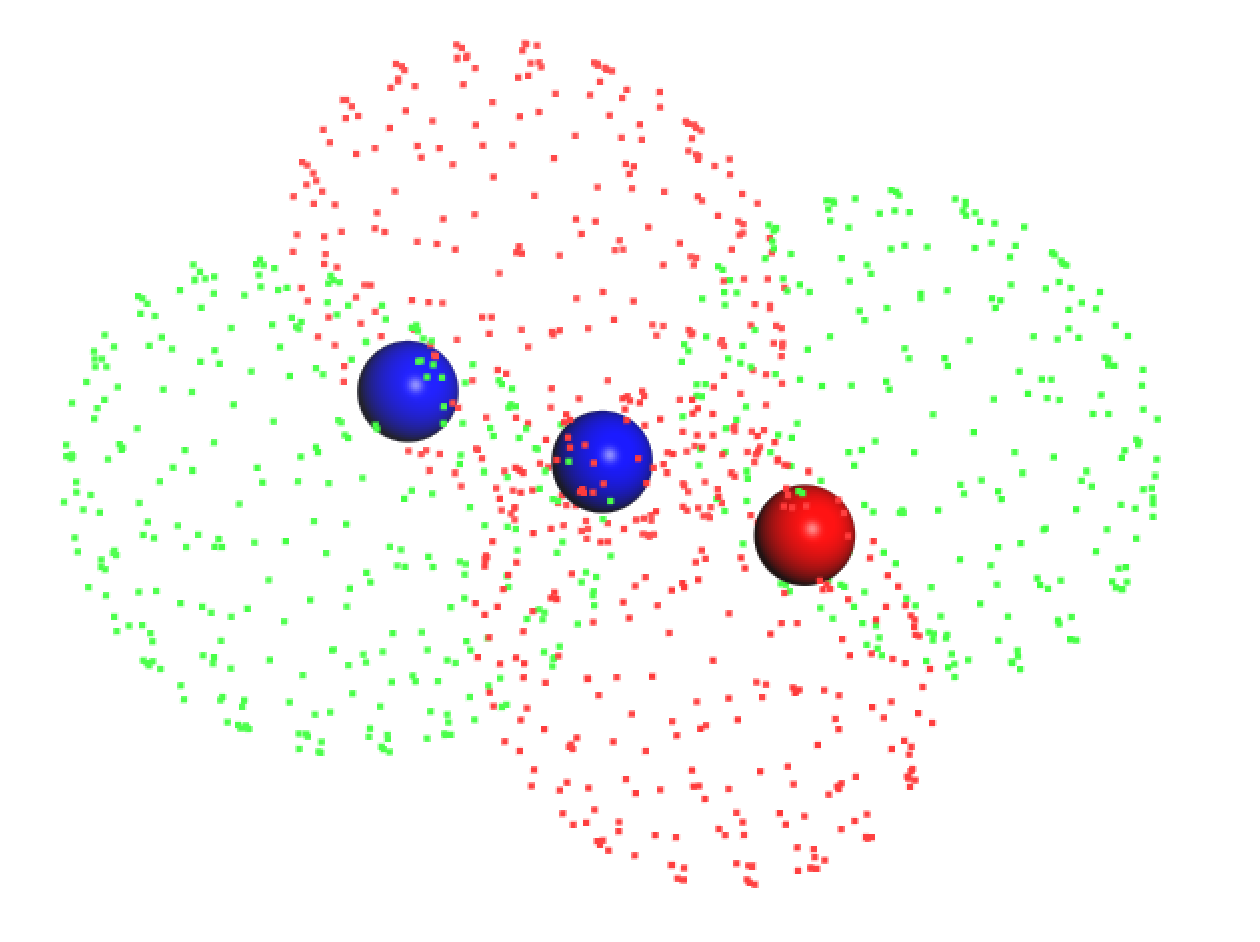
\includegraphics[width=\textwidth]{N2OHOMO.png}
        \caption{N\(_2\)O HOMO}
        \label{fig:n2o}
    \end{subfigure}
    \hfill
    \begin{subfigure}[b]{0.3\textwidth}
        \centering
        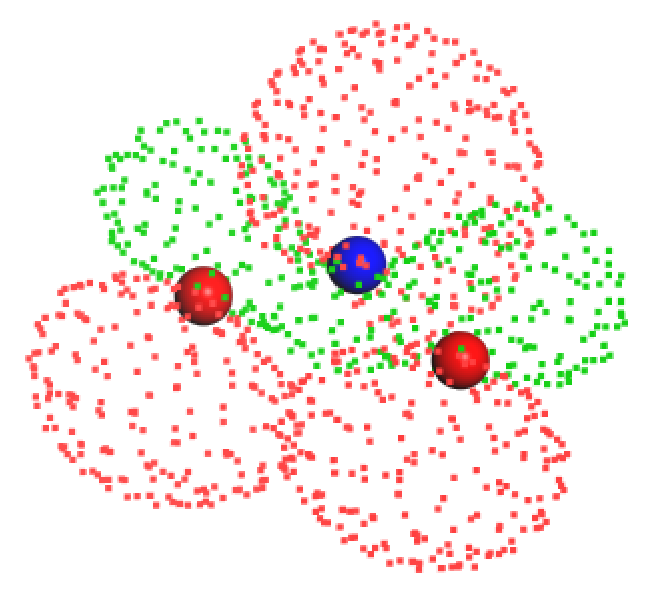
\includegraphics[width=\textwidth]{NO2HOMO.png}
        \caption{NO\(_2\) HOMO}
        \label{fig:no2}
    \end{subfigure}
    \caption{HOMO电子云图：NO，N\(_2\)O，NO\(_2\)}
    \label{fig:homo}
\end{figure}

\subsubsection{含硫氧化物}


\subsection{含氧酸}

在谈论具体的反馈键之前，让我们先环顾一下元素周期表。
你会发现，\textbf{p 区元素}——尤其是那些坐在周期表右侧的家伙们——
在含氧酸的舞台上出奇地活跃。
硫酸、磷酸、氯酸、硅酸……
这张名单可以一直列下去，而里面的主角几乎无一例外地来自 p 区。
这并非巧合。
这些元素天生就处在一个有趣的“边缘地带”：
它们的电负性足以稳定地与氧结合，
却又保留着足够灵活的空轨道来接纳电子的“回赠”。
正是这种微妙的平衡，使得 p 区元素成了含氧酸化学里不折不扣的明星。
现在，让我们来看看它们招牌动作背后的秘密——那个被称为“反馈 $\pi$ 键”的电子舞蹈。

\subsubsection{\texorpdfstring{$d$-$p\pi$}{d-p pi}反馈键：一个微妙的电子舞蹈}

现在我们来讨论一个更精细的量子力学效应。在第三周期及之后的原子形成的分子中，化学家们常常谈论所谓的“$d$-$p\pi$ 反馈键”。这个名字听起来像是一个神秘的咒语，但让我们看看它到底是什么意思。

本质上，这是一个关于电子如何“回流”的故事。想象一个中心原子，比如硅、磷、硫或氯，它处在一个较高的氧化态，周围被氧、氮或卤素这样的配体包围。按照简单的$\sigma$键图像，配体会慷慨地提供电子对，与中心原子形成共价键。但故事到这里并没有结束。这些配体，特别是那些带有孤对电子的，发现中心原子其实并非那么“电子满足”——它有一些空着的、能量上可以接受的$d$轨道。于是，一种奇妙的舞蹈开始了：配体上的一部分孤对电子，它们的电子云不只是待在原地，而是会微妙地“漏”向、或者说“反馈”给中心原子的那些空$d$轨道。因为这种侧向重叠的对称性类似于一个$\pi$键，但又是由$d$和$p$轨道构成的，所以我们就叫它$d$-$p\pi$ 反馈键。

要让这个反馈机制起作用，大自然开出了几个条件，就像一张严格的舞会请柬：

\begin{enumerate}
  \item \textbf{中心原子必须有“空位”。} 这并不是说它真的有一个空座位，而是说它必须具备能量足够低、能够接纳外来电子密度的空轨道。
  
  \item \textbf{捐赠者和接收者的能量要谈得拢。} 配体上的孤对电子有它们自己的能级，中心原子的空轨道也有它的能级。O、N、卤素这些配体的孤对电子，恰好常常和许多中心原子的空$d$轨道能级相近，所以它们成了绝佳的搭档。
  
  \item \textbf{几何上要“对得准”。} 轨道重叠不是随随便便的。要让$p$轨道的侧面和$d$轨道有好的重叠，它们的朝向必须匹配。
  
  \item \textbf{电荷的驱动力。} 中心原子上正电荷越多——或者说它越“贫电子”——它吸引配体上那些孤对电子云的本领就越强。
\end{enumerate}


现在我们要触及一个化学家们非常关心的问题：这种电子的微妙回流，怎么改变一个含氧酸的酸性强度？

想象一个含氧酸，比如$\mathrm{H_2SO_4}$或$\mathrm{HClO_3}$。它有一个$\mathrm{O}$--$\mathrm{H}$键，当这个键断裂、释放出质子的时侯，剩下的那个负离子——共轭碱——需要稳定住那个多出来的负电荷。如果这个负电荷能舒服地分散到整个离子上，不那么局促地堆在一个氧原子上，那么酸就会更强，因为它更愿意释放质子。

反馈$\pi$机制正是这样一个了不起的“分散大师”。当配体氧上的孤对电子向中心原子的空$d$轨道反馈时，整个体系的电子云被重新分配了。这通常会使得共轭碱中的负电荷更加离域，散布到更大的空间范围去。结果呢？共轭碱变得更稳定，酸性因此增强。

但这里有一个微妙的转折，我们必须诚实地说出来。如果反馈作用变得太强，导致中心原子几乎“吃饱”了电子，它的电子贫乏状态被大大缓解，那么它拉动$\mathrm{O}$--$\mathrm{H}$键电子对的能力反而可能下降。在这种情况下，酸性未必一味增强。大自然总是这样——从来不是单一因素说了算。实际的酸性，是由诱导效应、共振离域、溶剂化作用三方共同协商决定的。反馈键是这场协商中一个重要的声音，但不是唯一的声音。


电子的行为虽然看不见摸不着，但它会在分子结构上留下清晰的脚印。如果你能测量键长、观察分子的形状，你会看到这些证据：

\begin{enumerate}
  \item \textbf{键长会缩短，单键和双键的差别会变小。} 在没有反馈的时候，你预期中心原子和配体氧之间是一个典型的单键，旁边可能还有一个典型的双键。但反馈作用一来，单键获得了一些双键的特征，双键也匀出了一些电子密度。于是键长变得介于单键和双键之间——一种键级的“平均化”发生了。在硫酸根、磷酸根这些离子里，所有$\mathrm{S}$--$\mathrm{O}$或$\mathrm{P}$--$\mathrm{O}$键等长，就是最好的见证。
  
  \item \textbf{分子倾向于“躺平”。} 因为这种反馈要求轨道之间良好的侧向重叠，分子自然会倾向于采取平面的、或至少是近共平面的构型，好让反馈最大化。一旦分子躺平了，绕着键的自由旋转也就被抑制了——就像一扇门被额外加了一个铰链固定住。
  
  \item \textbf{在多配位阴离子中，等效键增多，电荷弥漫开来。} 在$\mathrm{ClO_4^-}$、$\mathrm{SO_4^{2-}}$、$\mathrm{PO_4^{3-}}$这些离子里，你找不到哪一个氧原子“独自”承担多余的负电荷。反馈机制让所有氧原子在对称性上是等价的，负电荷被均匀地涂抹在整个离子的表面上。这对于理解它们的反应性和稳定性至关重要。
\end{enumerate}

\subsubsection{含氯酸}


好了，理论讲了不少，现在我们也要介绍这个理论所对应的经验定理了。我们来看看一个具体的家族——氯的含氧酸。这是一组漂亮的例子，可以让我们把刚才讨论的那些原理放在一起检验。

氯形成一整个系列的含氧酸：
$$
\mathrm{HClO,\quad HClO_2,\quad HClO_3,\quad HClO_4}
$$
对应的氯氧化态依次是$+1,+3,+5,+7$。你看，氯的氧化态在逐步升高，周围那些不与氢相连的端氧原子数目也在增加。这给了我们一个绝佳的对比序列。

实验事实很清楚：
$$
\mathrm{HClO < HClO_2 < HClO_3 < HClO_4}
$$
酸性依次递增。为什么？从我们刚才讨论的角度看，原因至少有两条。第一，随着中心氯的氧化态升高，它的电负性有效值也在增大，对$\mathrm{O}$--$\mathrm{H}$键电子对的诱导拉力更强。第二，也是更重要的，非羟基氧的数目增加了。每一个非羟基氧都是一扇新的窗户，让反馈$\pi$机制有更多机会把负电荷从共轭碱中拉走、离域开来。$\mathrm{ClO_4^-}$中四个氧等价，负电荷被分摊得不能再舒服了，所以$\mathrm{HClO_4}$几乎是一个完全解离的强酸。

我必须在这里插一句提醒。化学初学者常常把“酸性强”和“氧化性强”混为一谈。在氯的含氧酸系列里，情况恰好是反过来的：酸性最弱的$\mathrm{HClO}$，反而是动力学上最活泼的氧化剂；而酸性最强的$\mathrm{HClO_4}$，在常温下却可以安安静静地待在瓶子里。热力学稳定性、动力学反应活性、酸性强度，这是三个不同的剧本，需要分开来读。不要让大脑自动把它们画上等号。

谈到含氧酸的酸性，就不能不提莱纳斯·鲍林——一位对化学键本质有着惊人直觉的人物。他总结过一个简单得让人愉快的经验规则。对于一般的含氧酸，第一步解离的$\mathrm{p}K_a$可以大概这样估算：
$$
\mathrm{p}K_{a1}\approx 8-5m
$$
这里的$m$是什么呢？非常直接：它就是“不与氢相连”的端氧原子数目（羰基氧）。让我们用这个规则来检验氯的含氧酸家族：$\mathrm{HClO}$的$m=0$，预计$\mathrm{p}K_a\approx 8$；$\mathrm{HClO_2}$的$m=1$，预计$\mathrm{p}K_a\approx 3$；$\mathrm{HClO_3}$的$m=2$，预计$\mathrm{p}K_a\approx -2$；$\mathrm{HClO_4}$的$m=3$，预计$\mathrm{p}K_a\approx -7$。趋势完全正确，而且数量级也大致合理。

当然，如果你去查精确的实验值，会发现偏差。这没什么好惊讶的。这个规则忽略了溶剂化能的细节、忽略了离子强度、忽略了温度。把它当作一个趋势判断的指南针就好——它能告诉你朝哪个方向走，但别指望它给出精确到小数点后两位的坐标。

\subsubsection{含硫酸}

如果说氯的含氧酸是一个井然有序的家族，那么硫的含氧酸就是一个关系更复杂、花样更多的亲戚群。硫形成的含氧酸种类繁多，我们来挑几个有代表性的：
$$
\mathrm{H_2SO_3,\quad H_2SO_4,\quad H_2S_2O_3,\quad H_2S_2O_7}
$$
这里面有简单的单核酸，也有通过硫-硫键或桥氧连接起来的“缩合”结构。每一种都有自己独特的电子结构和化学行为。



这个对比直接又清晰。$\mathrm{H_2SO_4}$中的硫氧化态是$+6$，被四个氧包围，其中两个是非羟基氧。按照鲍林规则，$m=2$，我们预期它是一个强酸——事实正是如此，它的第一步解离几乎完全。$\mathrm{H_2SO_3}$呢？硫的氧化态是$+4$，只有一个非羟基氧，$m=1$，酸性明显要弱。

但亚硫酸还有一个额外的复杂性：它在水中其实和溶解的$\mathrm{SO_2}$存在平衡，并不全以$\mathrm{H_2SO_3}$分子形式存在。大自然又一次提醒我们：不要把写在纸上的分子式当成溶液里真实发生的全部故事。


更有趣的是$\mathrm{H_2S_2O_3}$（硫代硫酸）和$\mathrm{H_2S_2O_7}$（焦硫酸）。前者可以看作硫酸根中的一个端氧被硫原子取代——一个$\mathrm{S}$--$\mathrm{O}$变成了$\mathrm{S}$--$\mathrm{S}$。这个末端硫和中心硫的电子环境截然不同，造成了有趣的化学反应性差异，尤其是在配位化学和氧化还原反应中。

后者$\mathrm{H_2S_2O_7}$则是两分子硫酸脱去一分子水缩合而成的。一个氧原子变成桥氧，连接两个硫中心。缩合之后，整个分子的电子结构改变了，酸性行为也随之调整——这提醒我们，氧在这些体系中不只是配位者，它还是优秀的连接者。

对于硫的含氧酸，大原则仍然站得住：中心氧化态越高、非羟基氧数目越多，酸性通常越强。但一旦分子结构变得复杂——出现了硫-硫键、桥氧连接、末端基团差异——这些额外的因素就会登台亮相，各自施加它们对电子密度分布、溶剂化和反应性的影响。好的化学理解，就是在掌握大原则的同时，也对这些“添乱的细节”保持敬意。

\subsubsection{含磷酸}

与硫的含氧酸类似，磷的含氧酸也展现出丰富的结构多样性，尤其以缩合程度不同而形成的各种多聚磷酸为特征。我们先列出几种代表性的磷酸：
$$
\mathrm{H_3PO_4,\quad H_3PO_3,\quad H_4P_2O_7,\quad H_5P_3O_{10}}
$$
这里面既有简单的单核酸，也有通过桥氧原子连接多个磷中心形成的缩合酸。

磷的含氧酸在结构上有一个区别于硫的显著特征：磷几乎总是以四配位形式存在，形成磷氧四面体。$\mathrm{H_3PO_4}$中磷的氧化态为$+5$，含有一个非羟基氧。按鲍林规则，$m=1$，预期为中强酸，这与实验事实一致——磷酸的$pK_{a1}\approx2.1$，属于中等强度的酸。

$\mathrm{H_3PO_3}$（亚磷酸）的情况则值得注意。虽然分子式写为$\mathrm{H_3PO_3}$，但它的实际结构是$\mathrm{HP(O)(OH)_2}$，含有一个直接键合在磷上的氢原子，即P--H键。这意味着三个氢中只有两个是酸性羟基氢，因此亚磷酸是二元酸而非三元酸。这一结构特征在命名简写时容易被忽略，却是理解其酸性和反应性的关键。

缩合磷酸是磷含氧酸中极为重要的一类。$\mathrm{H_4P_2O_7}$（焦磷酸）由两分子磷酸脱去一分子水缩合而成，通过一个桥氧原子连接两个磷中心。$\mathrm{H_5P_3O_{10}}$（三聚磷酸）则含有三个磷原子和两个桥氧连接。缩合后，每个磷原子仍保留自身的非羟基氧，因此分子整体的非羟基氧数目增加。按照鲍林规则的思路，缩合程度越高，第一级解离的酸性通常越强——链状多聚磷酸的酸性确实强于正磷酸，例如焦磷酸的$pK_{a1}\approx0.8$，三聚磷酸的$pK_{a1}\approx0.6$。

对于磷的含氧酸，大原则仍然成立：中心原子的氧化态越高、非羟基氧数目越多，酸性越强。亚磷酸中P--H键的存在提醒我们，分子式中氢原子的数目并不总是等于可解离的质子数，结构信息不可或缺。缩合磷酸则进一步体现了桥氧在整个聚阴离子结构中对电荷离域和酸性增强的贡献。这些结构因素共同构成了磷含氧酸丰富的化学行为。

\newpage


% ---- chunk ch2_9 : 2.x D区DS区 ----



\section{D区和DS区}

\subsection{副族元素的一般原理：电子结构、变价与配位}

副族元素涵盖D区与DS区，其共同特征在于价电子填充主要发生在$(n-1)d$轨道，同时伴随$ns$轨道参与成键。与$s$区和$p$区主族元素相比，副族元素的化学行为呈现出氧化态多样、配位化学丰富、化合物颜色变化显著以及磁性、催化活性与电子排布关系密切等系统性差异。

然而，D区与DS区在电子结构和化学性质上存在重要区别，有必要首先加以界定。

\subsubsection{D区与DS区的结构区分}

D区元素是指价电子依次填充$(n-1)d$轨道的过渡金属，其原子或离子的$d$轨道处于部分填充状态，典型代表如第一过渡系的Ti至Ni。DS区则指价层电子构型接近或达到$(n-1)d^{10}ns^{1\sim 2}$的元素区域，典型代表为IB族（Cu、Ag、Au）和IIB族（Zn、Cd、Hg）。二者的根本差异在于：D区元素的$(n-1)d$轨道未充满，成键时$d$电子可直接参与，从而表现出多种氧化态和丰富的$d$--$d$跃迁光谱；DS区元素的$d$轨道已充满，$d^{10}$电子组态主要表现为弱屏蔽和高极化率，成键时主要动用$ns$电子，$d$电子相对化学惰性，由此导致氧化态分布更为集中、水合离子多为无色以及与软配体的亲和力更强等特征。

DS区氧化态分布相对集中，可用$d^{10}$组态的稳定性加以理解。因为$d$轨道已满，高氧化态的形成需要动用已被相对论效应稳定化的$ns$电子，这在能量上不利。沿Zn、Cd、Hg顺序，相对论效应对$6s$轨道的收缩稳定化作用最强，导致Hg的化学行为与Zn、Cd存在明显差异——倾向于保留$6s^2$电子对、$+1$氧化态以$\mathrm{Hg_2^{2+}}$形式稳定存在、$+2$氧化态具有强氧化性等，均可由此得到统一解释。

再者，DS区元素与软配体的强亲和力，源于$d^{10}$电子组态的弱屏蔽效应使阳离子有效核电荷较高，极化能力强，同时$d$轨道的扩展有利于与软碱配体形成有效共价重叠。这一倾向沿Zn、Cd、Hg的顺序增强，与相对论效应导致的$d$轨道扩展趋势一致。


正是这一轨道填充度的差异，使D区与DS区在颜色规律、氧化态分布、配位倾向和键型特征上构成了系统的对照。以下先以D区为主讨论副族元素的一般结构和物理性质，再适时引入DS区的对比。

\subsubsection{副族元素的原子结构与物理性质}

从原子结构角度看，副族元素表现出几个共同的周期趋势。原子半径沿各过渡系呈现“前段明显减小、后段变化趋缓甚至略回升”的规律，这与$d$电子逐个填充时核电荷增加和屏蔽效应不完全之间的竞争有关。\ref{fig:ibdr}电负性总体沿周期上升，但因$d$电子填充对有效核电荷的影响并非线性，常出现局部回落，不如主族元素那样严格单调。\ref{fig:ibdi}

\begin{figure}[htbp]
    \centering
    \begin{subfigure}[b]{0.5\linewidth}
        \centering
        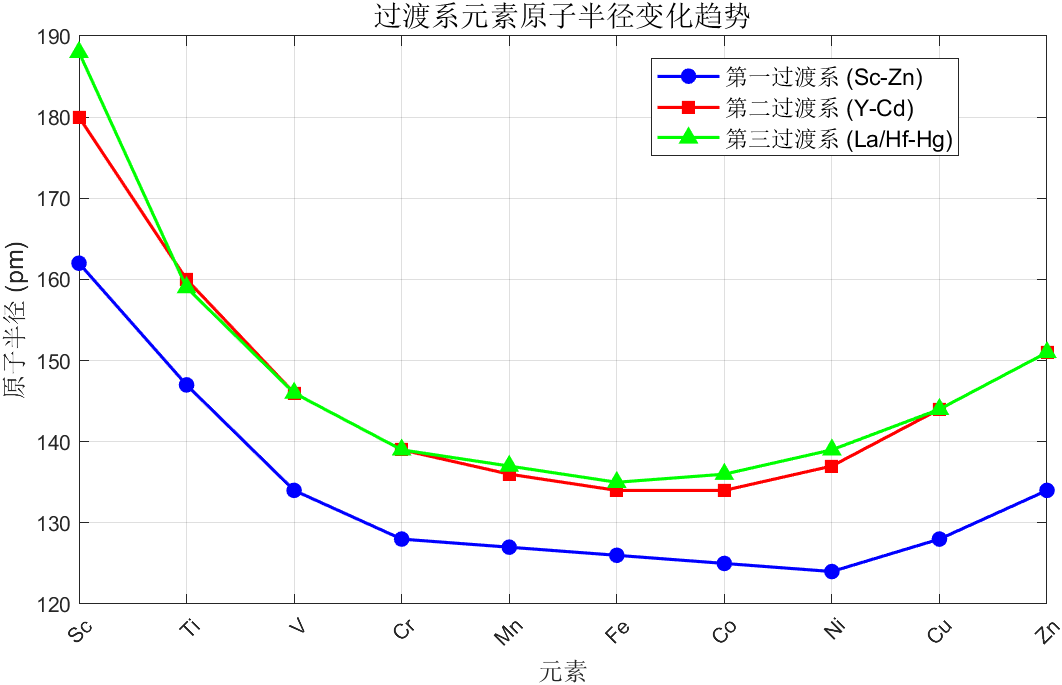
\includegraphics[width=\linewidth]{IBDR.png}
        \caption{IBDR}
        \label{fig:ibdr}
    \end{subfigure}%
    \begin{subfigure}[b]{0.5\linewidth}
        \centering
        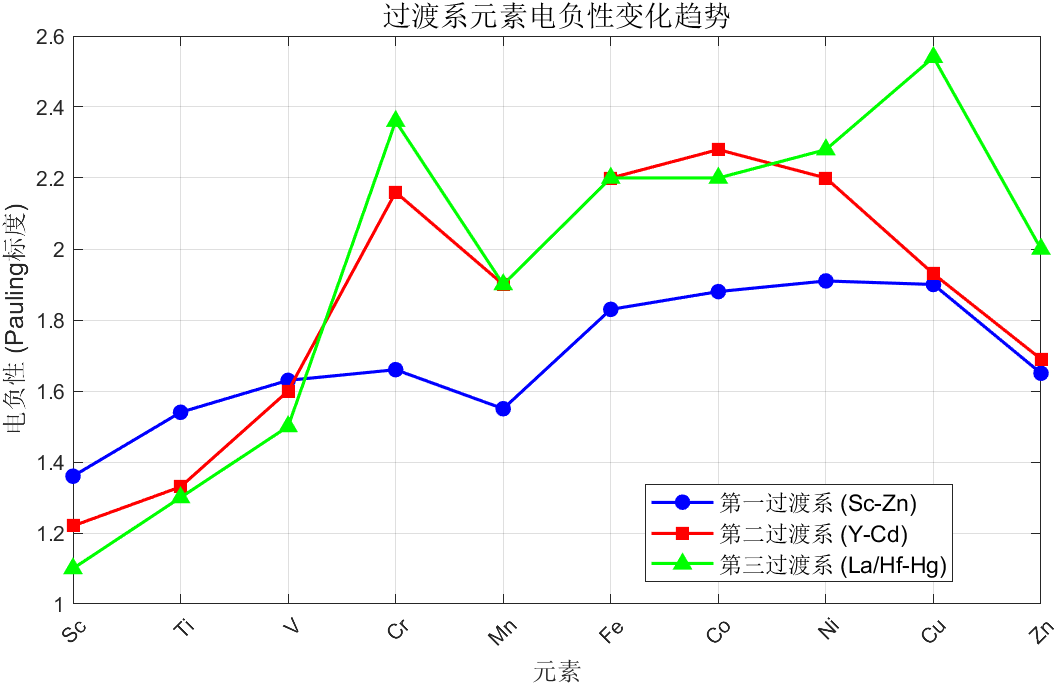
\includegraphics[width=\linewidth]{IBDI.png}
        \caption{IBDI}
        \label{fig:ibdi}
    \end{subfigure}
\end{figure}

对第一过渡系而言，$4s$与$3d$轨道的能级顺序在原子和离子中有所不同。在中性原子构造过程中，$4s$与$3d$能级非常接近，通常先填充$4s$后填充$3d$；但在形成阳离子后，$3d$轨道能量通常低于$4s$，因此失电子时往往先电离$4s$电子。这一“先填后失”的规律对理解过渡金属离子的电子构型至关重要。

电子排布方面，D区存在若干经典例外，其成因与半满和全满壳层的交换能增益以及$ns$与$(n-1)d$能级的极度接近有关。常见例子如下：

\medskip
\renewcommand{\arraystretch}{1.15}
\noindent\begin{tabular*}{\textwidth}{@{\extracolsep{\fill}}lll@{}}
\toprule
元素 & 按构造原理预期 & 实际基态排布 \\
\midrule
Cr & $[\mathrm{Ar}]\,3d^4 4s^2$ & $[\mathrm{Ar}]\,3d^5 4s^1$ \\
Cu & $[\mathrm{Ar}]\,3d^9 4s^2$ & $[\mathrm{Ar}]\,3d^{10} 4s^1$ \\
Nb & $[\mathrm{Kr}]\,4d^3 5s^2$ & $[\mathrm{Kr}]\,4d^4 5s^1$ \\
Mo & $[\mathrm{Kr}]\,4d^4 5s^2$ & $[\mathrm{Kr}]\,4d^5 5s^1$ \\
Ru & $[\mathrm{Kr}]\,4d^6 5s^2$ & $[\mathrm{Kr}]\,4d^7 5s^1$ \\
Rh & $[\mathrm{Kr}]\,4d^7 5s^2$ & $[\mathrm{Kr}]\,4d^8 5s^1$ \\
Pd & $[\mathrm{Kr}]\,4d^8 5s^2$ & $[\mathrm{Kr}]\,4d^{10} 5s^0$ \\
Ag & $[\mathrm{Kr}]\,4d^9 5s^2$ & $[\mathrm{Kr}]\,4d^{10} 5s^1$ \\
Pt & $[\mathrm{Xe}]\,4f^{14}5d^8 6s^2$ & $[\mathrm{Xe}]\,4f^{14}5d^9 6s^1$ \\
Au & $[\mathrm{Xe}]\,4f^{14}5d^9 6s^2$ & $[\mathrm{Xe}]\,4f^{14}5d^{10} 6s^1$ \\
\bottomrule
\end{tabular*}
\renewcommand{\arraystretch}{1.0}

这些例外说明，D区电子排布不能机械套用构造原理的填充顺序，必须同时考虑交换能稳定化以及$ns$与$(n-1)d$轨道能级接近带来的组态调整。

对于第二和第三过渡系元素，原子半径因镧系收缩而呈现一个重要的系统特征：$5d$元素的原子半径与同族$4d$元素十分接近，而非随周期增加而显著增大。\ref{fig:ibdr}这一效应对重过渡金属的化学性质具有深远影响，包括电离能增高、共价性增强以及某些贵金属化学惰性的出现。

\subsubsection{过渡金属离子的颜色与晶体场理论}

过渡金属化合物最直观的特征之一是其丰富的颜色表现。要理解这一现象的物理根源，需要引入晶体场理论的基本框架。

晶体场理论的核心假设是：在配位化合物中，配体被视为带负电荷的点电荷或偶极子，它们与中心金属离子的$d$电子发生静电排斥作用。由于$d$轨道具有不同的空间取向，在球形对称的自由离子中简并的五个$d$轨道，在配位场中会发生能级分裂。以八面体配合物为例，$d_{x^2-y^2}$和$d_{z^2}$轨道（合称$e_g$组）直接指向配体方向，受到的排斥较大，能量升高；$d_{xy}$、$d_{xz}$和$d_{yz}$轨道（合称$t_{2g}$组）的瓣指向配体之间的空隙，受到的排斥较小，能量降低。二者之间的能量差称为晶体场分裂能，记为$\Delta_{\mathrm{oct}}$或$10Dq$。

\begin{center}
  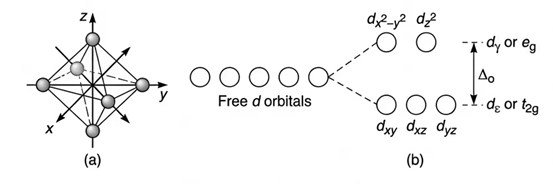
\includegraphics[width=0.9\textwidth]{Oct.png}
\end{center}

在四面体场中，情况就截然不同了。四个配体从立方体交替的四个顶点向中心离子靠近，此时坐标轴恰好从配体之间的空隙穿过。这样一来，$d_{xy}$、$d_{xz}$和$d_{yz}$轨道（在四面体对称性下记为$t_2$组）的瓣直接指向配体，受到的排斥大，能量升高；而$d_{x^2-y^2}$和$d_{z^2}$轨道（记为$e$组）反而指向配体之间的空隙，受到的排斥小，能量降低。分裂的图景恰好与八面体场上下颠倒。四面体场的分裂能记为$\Delta_{\mathrm{tet}}$，由于配体数只有四个，且没有配体直接正对着任何一条坐标轴，其分裂能远小于八面体场，理论值约为$\frac{4}{9}\Delta_{\mathrm{oct}}$。

\begin{center}
  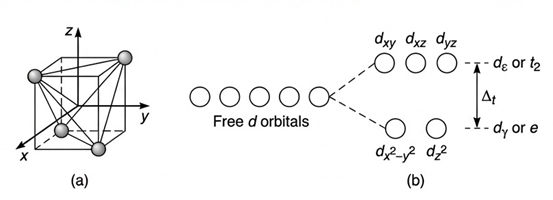
\includegraphics[width=0.9\textwidth]{Tetra.png}
\end{center}

现在到了平行四边形场，问题就变得微妙而精彩了。平面四边形配合物可以看作是八面体配合物沿$z$轴拉长的极端情形：轴向的两个配体逐渐远离，直至完全脱离，最终只在$xy$平面上留下四个配体。那么，如何理解从八面体场或四面体场到平行四边形场的畸变过程？这就需要请出姜-泰勒效应这个利器了。

\begin{center}
  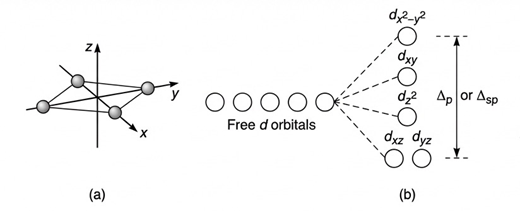
\includegraphics[width=0.9\textwidth]{Quad.png}
\end{center}

姜-泰勒定理告诉我们：在简并电子态下，非线性分子会发生几何畸变以解除简并、降低能量。对于$d^9$组态（如$\ce{Cu^2+}$）的八面体配合物，$e_g$轨道上电子占据不对称——两个简并轨道中，一个填充两个电子，另一个只填充一个电子，这就产生了简并电子态。系统为了稳定，会沿着某一坐标发生畸变。最常见的便是沿$z$轴拉长的八面体畸变：$z$方向配体远离，使含$z$分量的轨道（$d_{z^2}$、$d_{xz}$、$d_{yz}$）受到的排斥减弱，能量降低。分裂图景随之演化：原$e_g$组裂开，$d_{x^2-y^2}$能量大幅升高，$d_{z^2}$能量下降；$t_{2g}$组也裂开，$d_{xy}$因处于赤道平面而能量升高，$d_{xz}$和$d_{yz}$能量降低。若畸变程度较小，我们称之为小畸变，即仍可视为拉长的八面体，能级排序尚存八面体的影子；若轴向配体彻底离去，$d_{z^2}$的能量甚至低于$d_{xy}$，这便是大畸变，最终的极限就是平面四边形场。此时，四个配体在$xy$平面上沿$x$和$y$轴方向排列，$d_{x^2-y^2}$正对配体，能量飙至最高，$d_{xy}$次之，$d_{z^2}$和简并的$d_{xz}$、$d_{yz}$能量最低。这就是经典姜-泰勒畸变给出的八面体到平面四边形的路线图。

\begin{center}
  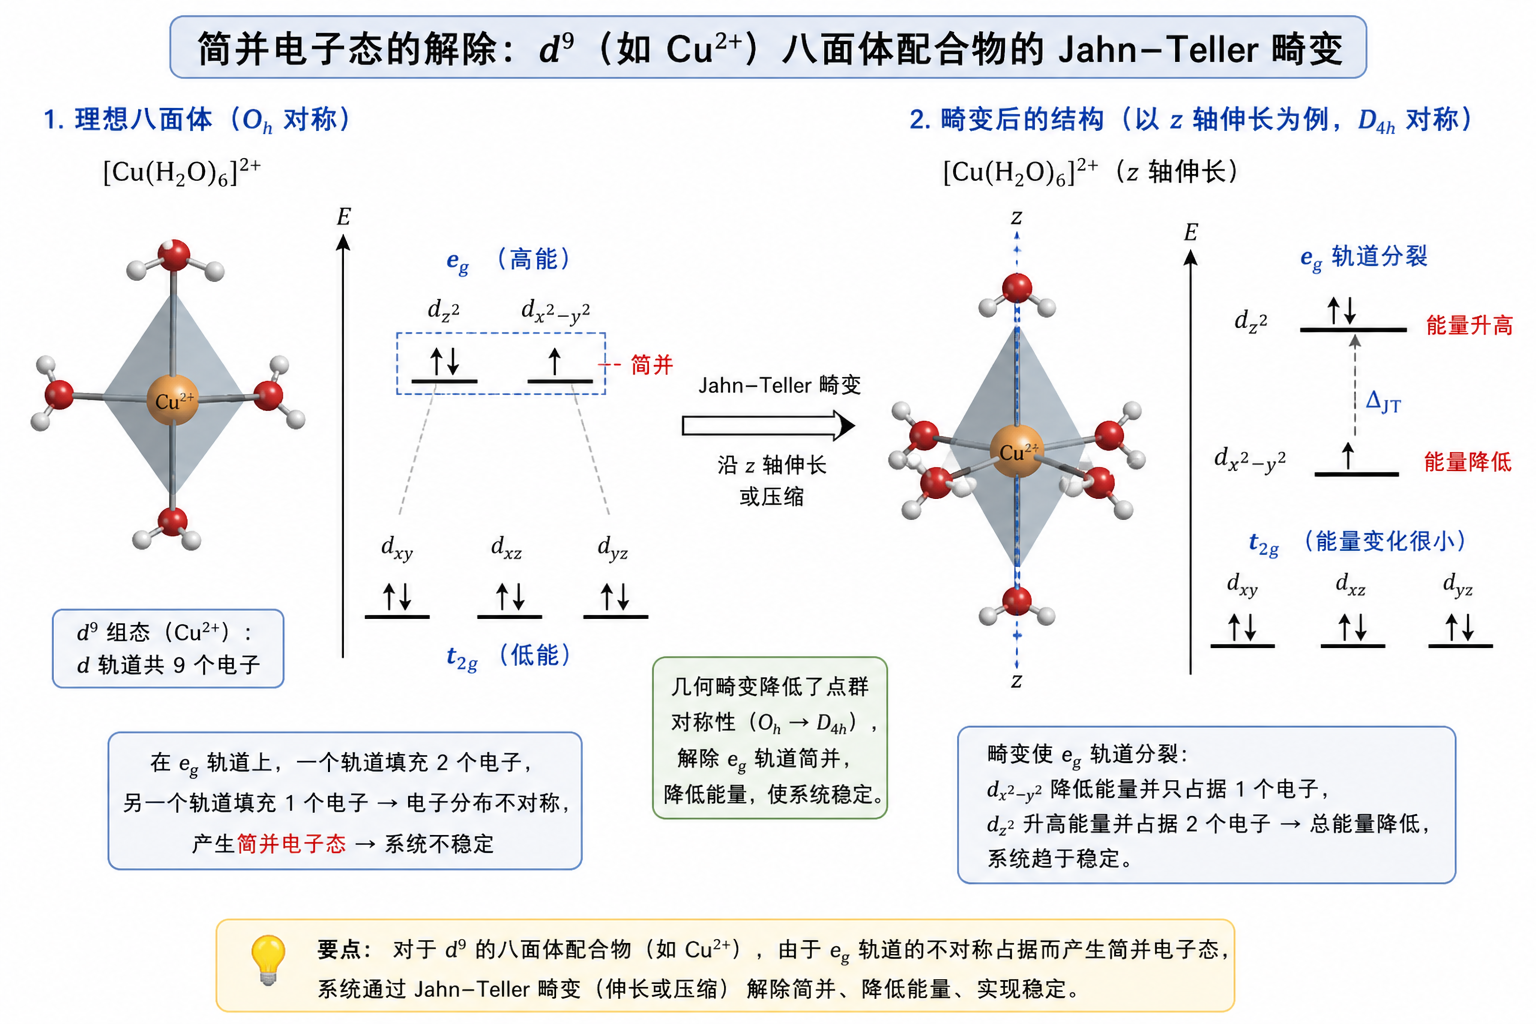
\includegraphics[width=\textwidth]{jtellereffect.png}
\end{center}

那么，四面体场也能畸变成四边形场吗？答案是肯定的，但逻辑不同。四面体配合物若发生姜-泰勒畸变——比如沿某个$S_4$轴压缩或拉伸——可以从四面体对称性逐步走向平面四边形。典型例子是某些$d^8$四配位配合物，既能以四面体构型存在，也能以平面四边形存在。畸变过程中，四面体的$t_2$和$e$轨道继续分裂，最终和平面四边形的能级图平滑衔接。

但是，这里必须辨析一个常见的误区：四边形场并不只由四面体场畸变而来。相反，在大多数常见的配合物化学中，平面四边形场更自然的前身是八面体场——通过失去轴向配体的极端姜-泰勒畸变而来。四面体到平面四边形的畸变虽然存在，却属于另一种对称性降低的路径。两种畸变殊途同归，最终都抵达$D_{4h}$对称性的平面四边形场，但它们的出发点和能级演化的中间过程完全不同。简而言之，四边形场是拉长的八面体和压扁的四面体在极端畸变下的共同归宿，但前一条路远比后一条常见得多，万不可认为四边形场只能由四面体而来。



这些能级分裂的直接后果是：当$d$轨道未完全填满时，电子可以在可见光的能量激发下从较低的$t_{2g}$能级跃迁到较高的$e_g$能级，即发生$d$--$d$跃迁。所吸收的光的波长取决于$\Delta$的大小，而透射或反射的光则呈现其互补色，这就是过渡金属离子呈现颜色的微观机制。

为系统地观察电子构型与颜色的关系，可将第一过渡系最常见的水合离子按$d$电子数排列如下：

\medskip
\renewcommand{\arraystretch}{1.15}
\noindent\begin{tabular*}{\textwidth}{@{\extracolsep{\fill}}ccccc@{}}
\toprule
$d$电子数 & 代表构型 & 常见阳离子 & 未成对电子数（高自旋） & 水合离子颜色 \\
\midrule
$d^0$ & $3d^0$ & $\mathrm{Sc^{3+}}$ & 0 & 无色 \\
$d^1$ & $3d^1$ & $\mathrm{Ti^{3+}}$ & 1 & 紫色 \\
$d^2$ & $3d^2$ & $\mathrm{V^{3+}}$ & 2 & 绿色 \\
$d^3$ & $3d^3$ & $\mathrm{Cr^{3+}}$ & 3 & 紫绿/绿色 \\
$d^4$ & $3d^4$ & $\mathrm{Mn^{3+}}$ & 4 & 紫色 \\
$d^5$ & $3d^5$ & $\mathrm{Fe^{3+}}$ & 5 & 黄色/棕黄色 \\
$d^6$ & $3d^6$ & $\mathrm{Fe^{2+}}$ & 4 & 浅绿色 \\
$d^7$ & $3d^7$ & $\mathrm{Co^{2+}}$ & 3 & 粉红色 \\
$d^8$ & $3d^8$ & $\mathrm{Ni^{2+}}$ & 2 & 绿色 \\
$d^9$ & $3d^9$ & $\mathrm{Cu^{2+}}$ & 1 & 蓝色 \\
$d^{10}$ & $3d^{10}$ & $\mathrm{Zn^{2+}}$ & 0 & 无色 \\
\bottomrule
\end{tabular*}
\renewcommand{\arraystretch}{1.0}

从该表可归纳出以下规律：

\begin{enumerate}
    \item \textbf{$d^0$和$d^{10}$构型一般无色}。前者无$d$电子，后者$d$轨道全满，均不发生$d$--$d$跃迁。因此$\mathrm{Sc^{3+}}$和$\mathrm{Zn^{2+}}$的水合离子无色。这一规律同样适用于DS区其他$d^{10}$离子如$\mathrm{Cd^{2+}}$和$\mathrm{Hg^{2+}}$。
    
    \item \textbf{$d$轨道未满时有色}。中间构型（$d^1$至$d^9$）在配位场中均可发生$d$--$d$跃迁，多数水合离子带有特征颜色。不同离子的颜色差异源于各$d^n$构型对应的基态与激发态能量差不同。
    
    \item \textbf{未成对电子数先增后减}。在高自旋八面体场中，从$d^0$到$d^5$未成对电子数逐步增至最大，从$d^6$到$d^{10}$再逐步减少。这一趋势与洪特规则在晶体场中的表现一致。
    
    \item \textbf{$d^9$构型与Jahn--Teller效应}。$\mathrm{Cu^{2+}}$（$d^9$）的八面体配合物常发生轴向拉长畸变，这是由于$e_g$轨道上电子占据不对称导致能级进一步分裂以降低体系能量。其水合离子呈蓝色，是这一构型的典型代表。
\end{enumerate}


在上述框架下，DS区元素的特殊性可得到系统说明。首先，DS区的$d^{10}$离子无色，正是晶体场理论的自然推演——无$d$--$d$跃迁意味着可见光区无吸收。若DS区化合物出现颜色，则其来源通常不是晶场分裂，而是配体-金属电荷转移跃迁或其它电子转移机制。

晶体场分裂不仅解释颜色，还对配合物的能量和磁性产生重要影响。晶体场稳定化能（CFSE）是指$d$电子在配位场分裂后的轨道中排布所获得的额外稳定化能量。对于给定$d^n$构型，电子在$t_{2g}$和$e_g$轨道上的分布方式取决于$\Delta$与电子成对能的相对大小，由此区分高自旋（弱场）和低自旋（强场）两种极限情况。

CFSE的大小直接影响配合物的热力学稳定性和动力学行为，也决定了未成对电子数，进而影响磁矩。多数第一过渡系水合离子处于高自旋态，未成对电子数与自由离子一致；强场配体（如$\mathrm{CN^-}$、$\mathrm{CO}$）则可迫使电子在$t_{2g}$上配对，形成低自旋配合物，使磁性显著降低甚至呈抗磁性。




综上，晶体场理论为理解副族元素——包括D区和DS区——的电子结构、颜色、磁性和配位行为提供了统一的理论框架。D区与DS区的差异，归根结底是$d$轨道填充程度不同所引起的系统性化学后果。

\newpage


% ===== [源文件缺失 ch2_10：源缺失] =====

% ---- chunk ch3_8 : DS区元素（顶替缺失的 ch2_11，标题一致） ----


\subsection{DS区元素}

这部分的元素可以从 Fajans 规则角度看，阳离子的极化能力主要与\textbf{电荷高、半径小、外层电子排布为18+2型、屏蔽差}有关。按理说作为18电子构型的元素，铜族元素的极化能力应该是普遍的强，但事实恰恰相反——铜离子是交界酸；金离子是极软的酸。这是因为电子构型带来的优势远不如松垮的 $d$ 电子带来的劣势。HSAB 理论本质上描述的还是电子云的变形性，虽然强极化力往往意味着紧缩的电子云，但是 $d$ 能级的放射状结构却不仅导致了屏蔽差，更使得难以有效收缩。

\subsubsection{铜银金}

铜族元素指：
\[
\mathrm{Cu,\ Ag,\ Au}
\]
它们最稳定的氧化态通常为 $+1$，对应离子分别为：
\[
\mathrm{Cu^+,\ Ag^+,\ Au^+}
\]
其价电子去除后通常形成封闭壳层或准封闭壳层，其中最常强调的是：\textbf{铜族一价离子都具有满 $d$ 壳层特征，可写作 $(n-1)d^{10}$，在配位与极化行为上表现出很强的特殊性。}

它们的化合物常呈现以下特征：
\begin{enumerate}
  \item 卤化物、硫化物和部分含氧酸盐具有比典型碱金属盐更强的共价性，且稳定性沿 $\mathrm{Cu<Ag<Au}$ 递变；
  \item 氢氧化物与氧化物常表现出\textbf{不稳定}，例如 $\mathrm{CuOH}$ 易分解为 $\mathrm{Cu_2O}$ 和水；
  \item 与软碱配体（如 $\mathrm{I^-}$、$\mathrm{S^{2-}}$、硫醚、硫脲、$\mathrm{CN^-}$ 等）结合较稳定，重元素 Ag、Au 这一趋势更明显；
  \item 在溶液化学中容易出现稳定络离子，如 $\mathrm{[Cu(CN)_2]^-}$、$\mathrm{[Ag(CN)_2]^-}$、$\mathrm{[Au(CN)_2]^-}$，以及 $\mathrm{[CuCl_2]^-}$、$\mathrm{[Ag(NH_3)_2]^+}$。
\end{enumerate}

对于较重元素，特别是 Au、Hg 以及更重的 $p$ 区元素，相对论效应已不再是微小修正，而会显著改变轨道能量与原子尺寸。其核心可概括为：\textbf{内层电子高速运动导致有效质量增加，使靠核较近的 $s$ 轨道发生收缩并稳定，而相应的 $d,f$ 轨道因屏蔽与正交效应表现为相对去稳定化和外扩。}

在铜族中，相对论效应沿族增强，可作如下理解：
\[
\mathrm{Cu < Ag < Au}
\]
其中 Au 最显著，因此 $\mathrm{Au^+}$、$\mathrm{Au^0}$ 与 $\mathrm{Au^{3+}}$ 都表现出比上方同族元素更特殊的成键行为与化学活性。对于金元素：
\begin{enumerate}
  \item Au 的 $6s$ 轨道受相对论效应强烈稳定，$6s$ 电子结合得异常紧；
  \item 结果使得 Au 的标准电极电势异常高，$\mathrm{Au^+}$ 具有很强的氧化性，而单质 Au 表现出极大的化学惰性（“真金不怕火炼”）；
  \item 同时 $5d$ 轨道因相对论效应发生扩缩与能级改变，使 Au(III) 配合物（如 $\mathrm{[AuCl_4]^-}$）呈现平面正方形构型，且金能与 $\mathrm{CO}$、$\mathrm{C_2H_4}$ 等分子形成稳定配合物，催化反应中表现独特。
\end{enumerate}

换言之，\textbf{金之所以“既是贵金属又不那么‘典型’”，根源就在于 $6s$ 电子被相对论效应过度稳定，使得 $+1$ 氧化态具有显著共价性和亲软性，同时 $+3$ 氧化态因 $d^8$ 构型而趋于平面四方形配位。}

\subsubsection{锌镉汞}

锌族元素指：
\[
\mathrm{Zn,\ Cd,\ Hg}
\]
它们最稳定的氧化态通常为 $+2$，对应离子分别为：
\[
\mathrm{Zn^{2+},\ Cd^{2+},\ Hg^{2+}}
\]
它们的化合物常呈现以下特征：
\begin{enumerate}
  \item 卤化物、硫化物和部分含氧酸盐具有比典型碱土金属盐更强的共价性；
  \item 氢氧化物与氧化物常表现出\textbf{两性}，例如 $\mathrm{Zn(OH)_2}$ 可溶于强酸也可溶于强碱；
  \item 与软碱配体（如 $\mathrm{I^-}$、$\mathrm{S^{2-}}$、硫醚、硫脲等）结合较稳定，重元素 Cd、Hg 这一趋势更明显；
  \item 在溶液化学中容易出现稳定络离子，如 $\mathrm{[Zn(NH_3)_4]^{2+}}$、$\mathrm{[CdCl_4]^{2-}}$、$\mathrm{[HgI_4]^{2-}}$。
\end{enumerate}

对于较重元素，特别是 Au、Hg 以及更重的 p 区元素，相对论效应已不再是微小修正，而会显著改变轨道能量与原子尺寸。其核心可概括为：\textbf{内层电子高速运动导致有效质量增加，使靠核较近的 $s$ 轨道发生收缩并稳定，而相应的 $d,f$ 轨道因屏蔽与正交效应表现为相对去稳定化和外扩。}

在锌族中，这惰电子对效应沿族增强，可作如下理解：
\[
\mathrm{Zn < Cd < Hg}
\]
其中 Hg 最显著，因此 $\mathrm{Hg^{2+}}$ 与中性 Hg 都表现出比上方同族元素更特殊的物态与成键行为。对于汞元素：
\begin{enumerate}
  \item Hg 的 $6s$ 轨道受相对论效应强烈稳定，$6s^2$ 电子结合得异常紧；
  \item 结果是 Hg--Hg 金属键显著减弱，晶格内原子间吸引不足；
  \item 因而汞的熔点异常低，在室温下呈液态，这是 DS 区最著名的相对论效应宏观体现之一。
\end{enumerate}

换言之，\textbf{汞之所以“像金属却不善于形成强金属键”，根源就在于 $6s$ 电子被相对论效应过度稳定，难以像普通金属价电子那样有效离域形成金属键。}





\newpage


% ---- chunk ch2_12 : D区元素化学（与 ch3_9 内容相同，取 ch2_12） ----



\subsection{D区元素化学：从钪组到锰族再到八族}

如果说主族元素像一排性格分明的“直线角色”，那么前五副族更像一组逐步展开的“连续人物”：从钪组开始，金属中心还比较“朴素”，高氧化态虽稳定但化学变化不算繁复；往右走到钛、钒、铬、锰族，$d$ 电子逐渐增多，氧化态、氧化还原、成簇倾向、含氧酸和配位行为便一层一层丰富起来。学习它们时，最重要的不是死记一长串化合物，而是抓住三条主线：\textbf{价态怎样变化、氧化物与含氧酸怎样对应、由轻到重时金属--金属成键和成簇能力怎样增强。}


把钪组到锰族并排看，可见一条清楚的横向主线：\textbf{最高氧化态随族序升高而升高}，由钪组的 +3 依次推进到锰族的 +7；\textbf{高价氧化物和含氧酸盐的重要性逐步增加}；\textbf{由 3d 向 4d/5d 过渡时，低价态金属--金属成键和成簇能力明显增强}；同时，\textbf{轻元素更善于在水溶液中表现颜色与变价，重元素更善于在固态和多核结构中“搭骨架”。}

\subsubsection{钪组：Sc, Y, La}

钪组元素常被看作过渡金属区的“起点”。它们最稳定、最重要的氧化态几乎都是\textbf{+3}，这一点一旦抓住，很多性质就会自动变得简单。对 Sc 而言，失去 $4s^2 3d^1$ 三个价电子后得到空的 $3d$ 壳层，形成 $\mathrm{Sc^{3+}}$；Y 和 La 也都同样偏爱三价。于是，这一族虽然站在 D 区里，却没有后面各族那样纷繁的变价行为。

从氧化物看，最典型的是\textbf{倍半氧化物} $\mathrm{M_2O_3}$，如 $\mathrm{Sc_2O_3}$、$\mathrm{Y_2O_3}$、$\mathrm{La_2O_3}$。它们整体上都偏\textbf{碱性}，且由 Sc 到 La，金属半径增大、离子键特征增强，氧化物碱性一般增强。换句话说，钪的氧化物还保留一点“边界感”，而到 Y、La 时，就更像典型电正金属的碱性氧化物了。它们与酸反应较易生成水合三价离子，而与强碱形成稳定酸根的倾向远不如后面高价态元素明显。

这一族的水合离子和盐类也很好理解。由于 $\mathrm{Sc^{3+}}$、$\mathrm{Y^{3+}}$、$\mathrm{La^{3+}}$ 半径较大、价电荷高，水溶液中易形成水合离子并发生一定程度水解，因此其盐类溶液常带一定酸性。它们的氢氧化物如 $\mathrm{Sc(OH)_3}$、$\mathrm{Y(OH)_3}$、$\mathrm{La(OH)_3}$ 溶解度都不大，体现出“三价硬酸 + 氢氧根硬碱”这一经典配对。

就元素比较而言，钪最轻、半径最小、极化能力也相对更强，因此其化学行为最容易带一点“过渡边缘”的味道；Y 与镧系前端元素则更明显表现出大半径三价阳离子的共同特征。至于\textbf{成簇与金属--金属键}，钪组并不算这方面的主角：因为它们几乎没有特别稳定的低氧化态可供停留，所以形成富电子金属簇的能力不如后面钼、钨、铼等元素突出。对大学生而言，可把钪组理解成：\textbf{D 区的门口，重点不在变价，而在稳定三价。}

\subsubsection{钛族：Ti, Zr, Hf}

到了钛族，情形立刻变得有意思起来。这里最鲜明的特征是：\textbf{+4 成为最稳定高氧化态，但低价态尤其是 +3 也仍有重要化学意义。}Ti 的常见氧化态有 +2、+3、+4，其中以 +4 最稳；Zr、Hf 则更明显偏向 +4，低价态稳定性较差。可以把它们想成“会向高氧化态上爬，但 Ti 还常常回头看看低价态世界”。

它们最重要的氧化物是\textbf{二氧化物} $\mathrm{TiO_2}$、$\mathrm{ZrO_2}$、$\mathrm{HfO_2}$。这些氧化物熔点高、热稳定性强、晶格坚固，体现出高价小半径金属对氧的强作用。$\mathrm{TiO_2}$ 是最熟悉的一个：白色、稳定、两性偏弱酸性，是重要颜料与光催化材料。$\mathrm{ZrO_2}$、$\mathrm{HfO_2}$ 则更突出耐火、耐高温与高介电常数特征。与主族元素那种“氧化物一见水就变酸或变碱”的直观印象不同，钛族高价氧化物往往更像坚固的三维网络固体。

钛族元素与酸碱反应的规律也很值得记住。Ti、Zr、Hf 在块体状态下都容易因表面致密氧化膜而表现出\textbf{钝化}，尤其对浓硝酸等氧化性介质较稳定；但在合适条件下，它们又能与氟离子形成稳定配阴离子，如 $\mathrm{[TiF_6]^{2-}}$、$\mathrm{[ZrF_6]^{2-}}$，这说明高价硬酸中心对 F 给体具有特别强的亲和力。于是，钛族化学常常一手抓“难溶难动的高价氧化物”，一手抓“在强配位环境中又能被拉入溶液的高配位络离子”。

从含氧酸角度说，钛族不像钒、铬、锰那样拥有一整套在水溶液中十分活跃的经典含氧酸体系，但可从“\textbf{高价氧化物在碱中形成氧酸盐或羟基络阴离子}”这个角度理解其弱酸性一面。Ti(IV) 在强碱或过氧体系中可形成钛酸盐或过氧络合物；Zr、Hf 更常以高配位羟基/氧桥体系存在。这里最重要的教学点不是背酸名，而是理解：\textbf{高电荷密度使它们更愿意形成 M--O 网络和多配位氧配合结构。}

钛族的元素对比中，Ti 最灵活，既有清晰的 +3 化学，又有大量分子或配位化学实例；Zr、Hf 则更“沉稳”，以 +4、难挥发、难还原、高配位和强亲氧性为主。由于镧系收缩，Zr 与 Hf 的半径非常接近，所以二者化学性质极相似，这几乎是教材中的经典例子。至于\textbf{成簇规律}，钛族已经比钪组更容易形成金属--金属相互作用与氧桥簇，但真正特别发达的金属簇化学还要到后面的钼、钨、铼去看。

\subsubsection{钒族：V, Nb, Ta}

钒族是学习“\textbf{价态阶梯}”最理想的一组。V 可以稳定地呈现 +2、+3、+4、+5 多种氧化态，溶液中甚至能靠颜色把这些价态一层层分出来；Nb、Ta 则虽然也能到 +5，但低价态在水溶液中不如 V 那样活泼鲜明。于是，这一族提供了一个极好的横向比较：\textbf{从轻到重，最高氧化态继续稳定，而低价态水溶液化学逐渐退居次要。}

先看氧化物。V 的氧化物非常典型：$\mathrm{VO}$、$\mathrm{V_2O_3}$、$\mathrm{VO_2}$、$\mathrm{V_2O_5}$ 分别对应较低到较高价态，酸碱与氧化还原性质也依次变化。尤其 $\mathrm{V_2O_5}$ 是典型高价氧化物，兼具氧化性和酸酐特征，可视作多钒酸、偏钒酸等体系的来源。Nb 与 Ta 的最重要氧化物则是 $\mathrm{Nb_2O_5}$、$\mathrm{Ta_2O_5}$，它们热稳定、难还原、偏酸性但在水中并不“活泼表演”，更常通过熔融碱、氟配位或复杂湿法体系体现其化学。

这一族最有教学价值的一个概念，是\textbf{含氧酸和多酸盐的缩合}。V(V) 在溶液中不是死板地只有一个离子，而会随 pH、浓度改变在偏钒酸根、焦钒酸根、多钒酸根之间转化。也就是说，这里开始出现一种新的思维：元素不是只给你一个“终极产物”，而是给你一整片彼此可互变的含氧阴离子家族。Nb、Ta 在这方面也能形成复杂氧酸盐与多核氧桥物种，只是溶液化学没有 V 那样鲜艳直观。

若把反应规律说得再简单一点，就是：\textbf{低价态偏还原，高价态偏氧化；高价态越往右、往下越稳，越容易形成难挥发、难溶或高配位氧化物/含氧阴离子。}V(V) 化合物常具氧化性，V(IV) 的 $\mathrm{VO^{2+}}$（钒酰离子）和 V(III)、V(II) 则更易参与还原过程。Nb、Ta 由于 +5 更稳，化学表现更集中在高价氧化物、卤配合物与氧酸盐体系上。

钒族最有教学价值的一点，是 V 在水溶液中能把“\textbf{价态变化伴随颜色变化}”展示得非常清楚，因此常被用来讲解过渡金属的变价行为。

\renewcommand{\arraystretch}{1.15}
\noindent\begin{tabular*}{\textwidth}{@{\extracolsep{\fill}}llll@{}}
\toprule
价态 & 代表离子/物种 & 典型颜色 & 性质特点 \\
\midrule
$+2$ & $\mathrm{V^{2+}}$ & 紫色 & 还原性很强，易被空气氧化 \\
$+3$ & $\mathrm{V^{3+}}$ & 绿色 & 仍具还原性，比 $\mathrm{V^{2+}}$ 稳定 \\
$+4$ & $\mathrm{VO^{2+}}$ & 蓝色 & 钒酰离子，较稳定，常见于酸性溶液 \\
$+5$ & $\mathrm{VO_2^{+}}$、钒酸盐 & 黄色/橙黄 & 氧化性增强，易形成多钒酸盐 \\
\bottomrule
\end{tabular*}
\renewcommand{\arraystretch}{1.0}

这张表说明两条规律：一是\textbf{价态越低，还原性越强}，所以 $\mathrm{V^{2+}}$ 最易被空气氧化；二是\textbf{价态越高，越倾向与氧形成稳定配位结构}，因此从 $\mathrm{V^{3+}}$ 到 $\mathrm{VO^{2+}}$、$\mathrm{VO_2^+}$ 再到钒酸盐，可以看到化学形态由简单阳离子逐渐转向含氧离子。

从教学上看，钒在溶液中的价态变化几乎可视作一条颜色楼梯：
\[
\mathrm{V^{2+}\,(紫) \rightarrow V^{3+}\,(绿) \rightarrow VO^{2+}\,(蓝) \rightarrow V(V)\,(黄)}
\]
实际颜色会受浓度、酸度和配位环境影响，并不总像教科书色卡那样整齐；但“紫--绿--蓝--黄”的序列仍很适合作为教学主线。

这也是钒族常被用来讲“价态阶梯”的原因：\textbf{氧化态变化不仅能写在式子里，也能在颜色和配位方式上直接看到。}相比之下，Nb、Ta 虽也有重要高价含氧物种，但在水溶液中不如 V 那样直观。

就\textbf{成簇与金属--金属成键}而言，V、Nb、Ta 都开始比前两族更具潜力，尤其 Nb、Ta 在卤化物和金属富集体系中可形成多核簇或金属链相互作用。这是因为随着周期变大，$d$ 轨道径向分布和金属中心尺寸更适合参与多中心成键。不过，如果只抓本科教材主线，那么对钒族最重要的仍是：\textbf{多价态、含氧酸盐、钒酰结构以及由 V 到 Nb/Ta 的高价态稳定化。}

\subsubsection{铬族：Cr, Mo, W}

铬族的主线很清楚：\textbf{+6 是全族的重要高氧化态，且由 Cr 到 Mo、W，高价态和金属--金属成簇能力都更稳定。}Cr 体现多变价与强氧化性，Mo、W 则进一步发展出更丰富的多酸盐与金属簇化学。

在氧化物方面，Cr 呈现从 $\mathrm{CrO}$、$\mathrm{Cr_2O_3}$、$\mathrm{CrO_2}$ 到 $\mathrm{CrO_3}$ 的完整梯度；其中 $\mathrm{Cr_2O_3}$ 是稳定的 Cr(III) 氧化物，$\mathrm{CrO_3}$ 则对应铬酸、重铬酸体系。Mo、W 最关键的高价氧化物是 $\mathrm{MoO_3}$、$\mathrm{WO_3}$，它们都是典型酸性氧化物，并进一步通向钼酸盐、钨酸盐及多酸盐化学。换言之，\textbf{铬族高价氧化物普遍走向含氧酸与氧桥阴离子体系。}

铬酸与重铬酸平衡是本科无机化学的“明星反应”之一：
\[
2\mathrm{CrO_4^{2-}} + 2\mathrm{H^+} \rightleftharpoons \mathrm{Cr_2O_7^{2-}} + \mathrm{H_2O}
\]
这条平衡说明，含氧酸根会随酸碱条件在不同聚合度之间切换。Mo、W 的多酸盐化学比 Cr 更发达，常见多钼酸根、多钨酸根乃至杂多酸，体现出高价金属通过氧桥构筑大骨架的趋势。

铬族的氧化还原规律也很有层次。Cr(VI) 是强氧化态，尤其在酸性下氧化性明显；Cr(III) 则稳定得多。Mo(VI)、W(VI) 虽然也是高氧化态，但它们在水溶液中不如 Cr(VI) 那样咄咄逼人，更多表现为稳定含氧阴离子与配位骨架。换句话说，\textbf{同是 +6，Cr 更像一个强氧化剂，Mo、W 更像高价、强 M--O 成键的骨架构筑者。}

在\textbf{成簇规律}上，Mo、W 尤其容易形成金属--金属多重键和多核簇，如 Mo--Mo 四重键体系、卤化物簇、硫化物簇和金属羰基簇。随着元素变重，$4d/5d$ 轨道更适合多中心成键，因此 Mo、W 的簇化学明显比 Cr 丰富。可概括为：\textbf{从 Cr 到 Mo、W，高价氧酸盐化学与多核金属簇化学并行增强。}

Cr 较难像 Mo、W 那样形成稳定而丰富的金属簇，主要因为三点：\textbf{3d} 轨道更紧凑，金属--金属重叠较弱；高价 Cr--O 化学尤其稳定，成键能力更倾向投入含氧体系；低价态又较不稳定，容易继续被氧化或歧化，因此可作为成簇前体的窗口较窄。

如果把这件事说得更“结构化”一些，可以做一个简短比较：

\renewcommand{\arraystretch}{1.15}
\noindent\begin{tabular*}{\textwidth}{@{\extracolsep{\fill}}lccc@{}}
\toprule
比较项目 & Cr & Mo & W \\
\midrule
主要参与成键轨道 & $3d$ & $4d$ & $5d$ \\
轨道径向分布 & 较紧凑 & 较外展 & 更外展 \\
高价含氧化学稳定性 & 很强 & 很强 & 很强 \\
金属--金属多重键/簇化学 & 相对较弱 & 很发达 & 很发达 \\
典型教材印象 & 铬酸/重铬酸 & 钼簇、多酸盐 & 钨簇、多酸盐 \\
\bottomrule
\end{tabular*}
\renewcommand{\arraystretch}{1.0}

这张表并不是说 Cr 不能形成金属--金属键，而是说：\textbf{在系统而丰富的多核簇化学上，Cr 明显不如 Mo 和 W 占优势。}对本科教学而言，可记成一句话：\textbf{Cr 更突出高价含氧化学；Mo、W 则在此基础上进一步发展出更强的多重键与金属簇化学。}

\subsubsection{锰族：Mn, Tc, Re}

锰族最能体现“氧化态丰富”这一特征。Mn 可出现从 +2 到 +7 的多种氧化态，其中 +2、+4、+7 最重要；Tc、Re 也能达到 +7，且高价含氧物种更稳定。其总规律是：\textbf{由 Mn 到 Tc、Re，低价态化学逐渐退居次要，高价态则更稳定并更偏向强 M{=}O 成键与含氧酸盐结构。}

Mn 的典型氧化物有 $\mathrm{MnO}$、$\mathrm{Mn_2O_3}$、$\mathrm{MnO_2}$ 和 $\mathrm{Mn_2O_7}$，其中 $\mathrm{MnO_2}$ 最关键：它是稳定的中间价态氧化物，也在氧化还原、催化和电池化学中占有中心地位。高锰酸根 $\mathrm{MnO_4^-}$ 对应 +7，是本科化学最经典的强氧化剂之一；其还原产物随介质而变：酸性多到 $\mathrm{Mn^{2+}}$，中性或弱碱性常到 $\mathrm{MnO_2}$，强碱性可到 $\mathrm{MnO_4^{2-}}$。

Tc 与 Re 的含氧化学更偏高价和稳定。高锝酸根 $\mathrm{TcO_4^-}$、高铼酸根 $\mathrm{ReO_4^-}$ 都是典型 +7 含氧阴离子，结构上与高锰酸根相似，但氧化性并不完全相同：Mn(VII) 更像积极的氧化剂，而 Re(VII) 常更稳定、更温和。这体现了同族向下的常见趋势：\textbf{高氧化态仍能保留，但氧化性未必同样强烈。}

锰族也很适合讲“价态演变”：Mn(II) 因半满 $d^5$ 高自旋而具有特殊稳定性；Mn(III) 常不稳定，易歧化或继续氧化还原；Mn(IV) 以 $\mathrm{MnO_2}$ 形式稳定；Mn(VI)、Mn(VII) 则进入高价含氧阴离子世界。Tc、Re 也保留了宽广价态范围，但教学重点通常更放在高价氧配位和多核金属化学上。

在\textbf{成簇规律}上，Tc、Re 尤其值得一提。Re 的多核羰基簇、金属--金属键和高价氧代配合物都很典型；Tc 也有丰富的配位与簇化学，只是因放射性，教学中多停留在概念层面。可概括为：\textbf{Mn 最适合讲氧化还原，Re 最适合讲高价氧配位与金属簇，而 Tc 介于两者之间。}


\subsubsection{八族}

\newpage



% ---- chunk ch9 : 第三章 有机化学（整章新块，替代旧 ch3 系列） ----

\chapter{有机化学}


键线式（skeletal structure）是我们最常使用的记号，它的出发点是一个约定：碳骨架用线段表示，碳原子本身不写。一条折线的端点和每个拐角都是一个碳，碳上的氢按四价自动补足，因此通常也省略。杂原子（O、N、S、卤素等）必须写出，连在杂原子上的氢也必须写出——因为“省氢”这条规则的适用对象只有碳。

把这条约定拆成可操作的六条：

\begin{enumerate}
  \item 线段的端点与折点是碳；线段本身是 \ce{C-C} 单键，双线是双键，三线是三键。
  \item 每个碳按四价补氢。画出的键少于四根时，缺的价数由氢补齐，但这些氢不写。
  \item 杂原子与杂原子上的氢必须显式写出，例如 \ce{-OH}、\ce{-NH_2}、\ce{-SH}。
  \item 电荷、孤对电子、未成对电子必须标出，它们往往正是反应发生的位置。
  \item 立体信息用实楔（朝向读者）与虚楔（背离读者）表示，普通实线表示位于纸面内。
  \item 缩写基团（\ce{Me}、\ce{Ph} 等）只是把一整块骨架折叠成一个标签，展开后仍按上述规则读。
\end{enumerate}

先看最简单的例子。丙烷的骨架是一条折线，两个端点和中间一个折点，共三个碳：
\begin{center}
\chemfig{-[:30]-[:-30]}
\qquad
\chemfig{CH_3-[:30]CH_2-[:-30]CH_3}
\end{center}
右式写全了碳和氢，左式只留骨架。两者是同一个分子，但左式把注意力留给了形状，右式把注意力留给了原子。异丁烷在中间那个碳上多分出一根线，这根线的端点就是第四个碳：
\begin{center}
\chemfig{-[:30](-[2])-[:-30]}
\qquad
\chemfig{CH_3-[:30]CH(-[2]CH_3)-[:-30]CH_3}
\end{center}
如果折点处的碳已经连了四根线，就不再补氢；如果只连了三根，就补一个氢；连了两根，补两个。这条“数键补氢”的规则要练到不看结构式也能在脑中完成。

环状化合物同样如此。环己烷是一个六元环，每个顶点是一个 \ce{CH_2}：
\begin{center}
\chemfig{*6(------)}
\qquad
\chemfig{*6(-=-=-=)}
\qquad
\chemfig{**6(------)}
\end{center}
左式画出六根单键，是环己烷；中式和右式都是苯——中式画出单双键交替的 Kekulé 式，右式在环内加一个圆圈，表示六个 $\pi$ 电子离域。芳香环的这两种画法在键线式中都通行，本书在需要强调“单双键交替”的机理场合用 Kekulé 式，在只强调芳香性时用圆圈式。

杂原子一旦出现，就必须写出。乳酸（2-羟基丙酸）的骨架如下，中间的折点连着一个 \ce{OH}，端点之一是羧基：
\begin{center}
\chemfig{-[:30](-[2]OH)-[:-30](=[-2]O)-[:30]OH}
\end{center}
但是有机化学中的官能团千千万，许多官能团都是以一个整体出现的，所以为了方便我们还规定了许多简写：

\begin{table}[H]
\centering
\caption{有机化学中常用的基团缩写}
\renewcommand{\arraystretch}{1.15}
\begin{tabular*}{\textwidth}{@{\extracolsep{\fill}}llll@{}}
\toprule
缩写 & 含义 & 缩写 & 含义 \\
\midrule
\ce{Me} & 甲基 \ce{CH_3} & \ce{Et} & 乙基 \ce{C_2H_5} \\
\ce{i-Pr} & 异丙基 & \ce{t-Bu} & 叔丁基 \\
\ce{Ph} & 苯基 & \ce{Bn} & 苄基 \ce{PhCH_2} \\
\ce{Ar} & 芳基 & \ce{Ac} & 乙酰基 \ce{COCH_3} \\
\ce{Bz} & 苯甲酰基 & \ce{Ts} & 对甲苯磺酰基 \\
\ce{Ms} & 甲磺酰基 & \ce{Tf} & 三氟甲磺酰基 \\
\ce{THF} & 四氢呋喃 & \ce{DMSO} & 二甲基亚砜 \\
\ce{DMF} & \ce{N,N}-二甲基甲酰胺 & \ce{Et_2O} & 乙醚 \\
\ce{LDA} & 二异丙基氨基锂 & \ce{NBS} & \ce{N}-溴代丁二酰亚胺 \\
\ce{mCPBA} & 间氯过氧苯甲酸 & \ce{DIBAL-H} & 二异丁基氢化铝 \\
\ce{TBS} & 叔丁基二甲基硅基 & \ce{TBAF} & 四丁基氟化铵 \\
\bottomrule
\end{tabular*}
\end{table}
这部分不必强行记忆，一般来说用的多了自然就记住了。

IUPAC 命名的核心是“选主链、定编号、写取代基”三步，但真正容易出错的是优先级。官能团的优先顺序大致为：羧酸 $>$ 酸酐 $>$ 酯 $>$ 酰卤 $>$ 酰胺 $>$ 腈 $>$ 醛 $>$ 酮 $>$ 醇 $>$ 胺 $>$ 醚 $>$ 卤代物。主链必须包含最高优先级的官能团；编号使该官能团位次最小；其余基团按字母序列出。

不饱和键的位次尽量小，若与官能团冲突则官能团优先。芳烃衍生物常用邻（o-）、间（m-）、对（p-）表示两个取代基的相对位置，多于两个取代基时改用编号。

杂环的命名另有一套 Hantzsch-Widman 规则，但常用杂环（吡啶、吡咯、呋喃、噻吩、咪唑、喹啉）直接记俗名更快。本书涉及杂环时一律用俗名，并在首次出现处画出结构。

\begin{center}
\chemfig{*6(-N=-=-=)}
\quad
\chemfig{*5(-N=-=)}
\quad
\chemfig{*5(-O-=-=)}
\quad
\chemfig{*5(-S-=-=)}
\end{center}

从左到右依次是吡啶、吡咯、呋喃、噻吩。注意吡咯的氮上有一个氢，它的孤对电子参与芳香体系；吡啶的氮上孤对电子在环平面内，不参与 $\pi$ 体系。这一差别决定了前者是弱酸（\ce{N-H} 可解离），后者是弱碱（氮孤对可质子化）。

一条反应箭头承载的信息比它看起来多。箭头上方写试剂，下方写溶剂、温度或催化剂；箭尾到箭头之间若有多步，用编号或分步箭头。平衡用 $\rightleftharpoons$，不可逆用 $\longrightarrow$。

\begin{center}
{\setchemfig{compound sep=8em}
\schemestart
\chemfig{-[:30]=[:-30]}
\arrow{->[\ce{HBr}][\ce{Et_2O}, $0\,^{\circ}\mathrm{C}$]}
\chemfig{-[:30](-[2]Br)-[:-30]}
\schemestop}
\end{center}

写反应式时有两个约定值得坚持：一是配平（碳数、电荷、副产物），二是标明立体化学（楔形键、E/Z、顺反）。很多“反应写对了但产物不对”的错误，根源都在立体化学没写清。

机理用弯箭头表示电子对的移动。双钩箭头（full arrow）表示一对电子，从键或孤对出发，指向形成新键的原子或断裂的键；鱼钩箭头（fishhook）表示单电子移动，用于自由基反应。箭头的尾巴必须落在电子所在的键或孤对上，箭头必须落在能接受电子的原子或键上——这两条是画机理的硬规则。

\begin{center}
\chemfig{@{a}C=[:30]@{b}C}
\chemmove{
  \draw[-{Stealth[length=2mm]}] ($(a)!0.5!(b)+(-0.02,-0.05)$) .. controls +(270:11mm) and +(315:11mm) .. ($(b)+(-0.04,-0.13)$);
}
\end{center}

上图表示 $\pi$ 键的一对电子流向右侧碳，形成一个新键。真实的加成反应还涉及亲电试剂，完整的箭头图会在下一章逐类展开。

反应坐标图上，中间体是能量谷，过渡态是能量峰。中间体可以被捕获、可以被光谱观测；过渡态不能，它只是势能面上的一个鞍点。判断一个反应是“协同”还是“分步”，就看图上有没有中间体这个谷。

动力学控制与热力学控制的区别也在这张图上：产物 A 生成得快但能量高，产物 B 生成得慢但能量低；低温停在前者，高温平衡到后者。共轭二烯的 1,2- 与 1,4- 加成就是最经典的例子。

碳的三种杂化（$sp^3$、$sp^2$、$sp$）决定了键角与 $\pi$ 键的有无。单键是 $\sigma$ 键，双键是一个 $\sigma$ 加一个 $\pi$，三键是一个 $\sigma$ 加两个互相垂直的 $\pi$。$\pi$ 电子云暴露在键轴上下，容易被亲电试剂进攻，这是烯烃、炔烃、芳烃反应性的共同来源。

键的极性来自两端的电负性差。\ce{C-O}、\ce{C-N}、\ce{C-X} 都有明显的偶极，碳端带部分正电荷，因此成为亲核试剂的进攻位点。羰基的极性最强，因为氧的电负性大且 $\pi$ 键可极化，这就是羰基化学几乎全是亲核加成的原因。

诱导效应沿 $\sigma$ 键传递，随距离迅速衰减，通常超过三根键就可以忽略。它改变的是电子云密度，不改变轨道形状。

共轭效应要求 $p$ 轨道或 $\pi$ 轨道彼此平行且能量接近。$p$-$\pi$ 共轭（如 \ce{-OH}、\ce{-NH_2} 与苯环）、$\pi$-$\pi$ 共轭（如 1,3-丁二烯）、$\sigma$-$\pi$ 超共轭（如烷基与碳正离子）都是同一件事：电子在更大的范围内离域，体系能量降低。

\begin{center}
\chemfig{=[:30]-[:-30]=[:30]}
\qquad
\chemfig{*6(-=(-OH)-=-=)}
\end{center}

左侧是 $\pi$-$\pi$ 共轭，右侧是 $p$-$\pi$ 共轭。共轭的方向由“谁更愿意给出电子”决定：氧、氮的孤对电子推向环内，是给电子共轭；羰基、硝基的 $\pi$ 键把电子拉走，是吸电子共轭。

\newpage


% ---- chunk ch9_2 : 3.x 空间异构（与 ch3_2 同内容） ----


\section{空间异构}

一般的$\sigma$键可旋转，所以一般具有极高的对称性，但是仍然有些特殊的情况，使得这些对称性破缺，虽然两个分子构成完全相同，但却实际上不一样，这就构成了空间异构。

\subsection{手性异构}


有机化学的一大复杂点就是分子的手性，两个构成完全相同的分子，却不是相同的，就像我们的左手与右手。键线式在表示此类手性化合物上存在先天的痛点，因为平面记号很难表示出三维的结构（大多数人空间想象力不好），虽然我们可以用楔形键来表示键伸展的方向，但是还是不好用，所以在这里我们一般用 Fischer 投影式。
\begin{figure}[htbp]
  \centering
  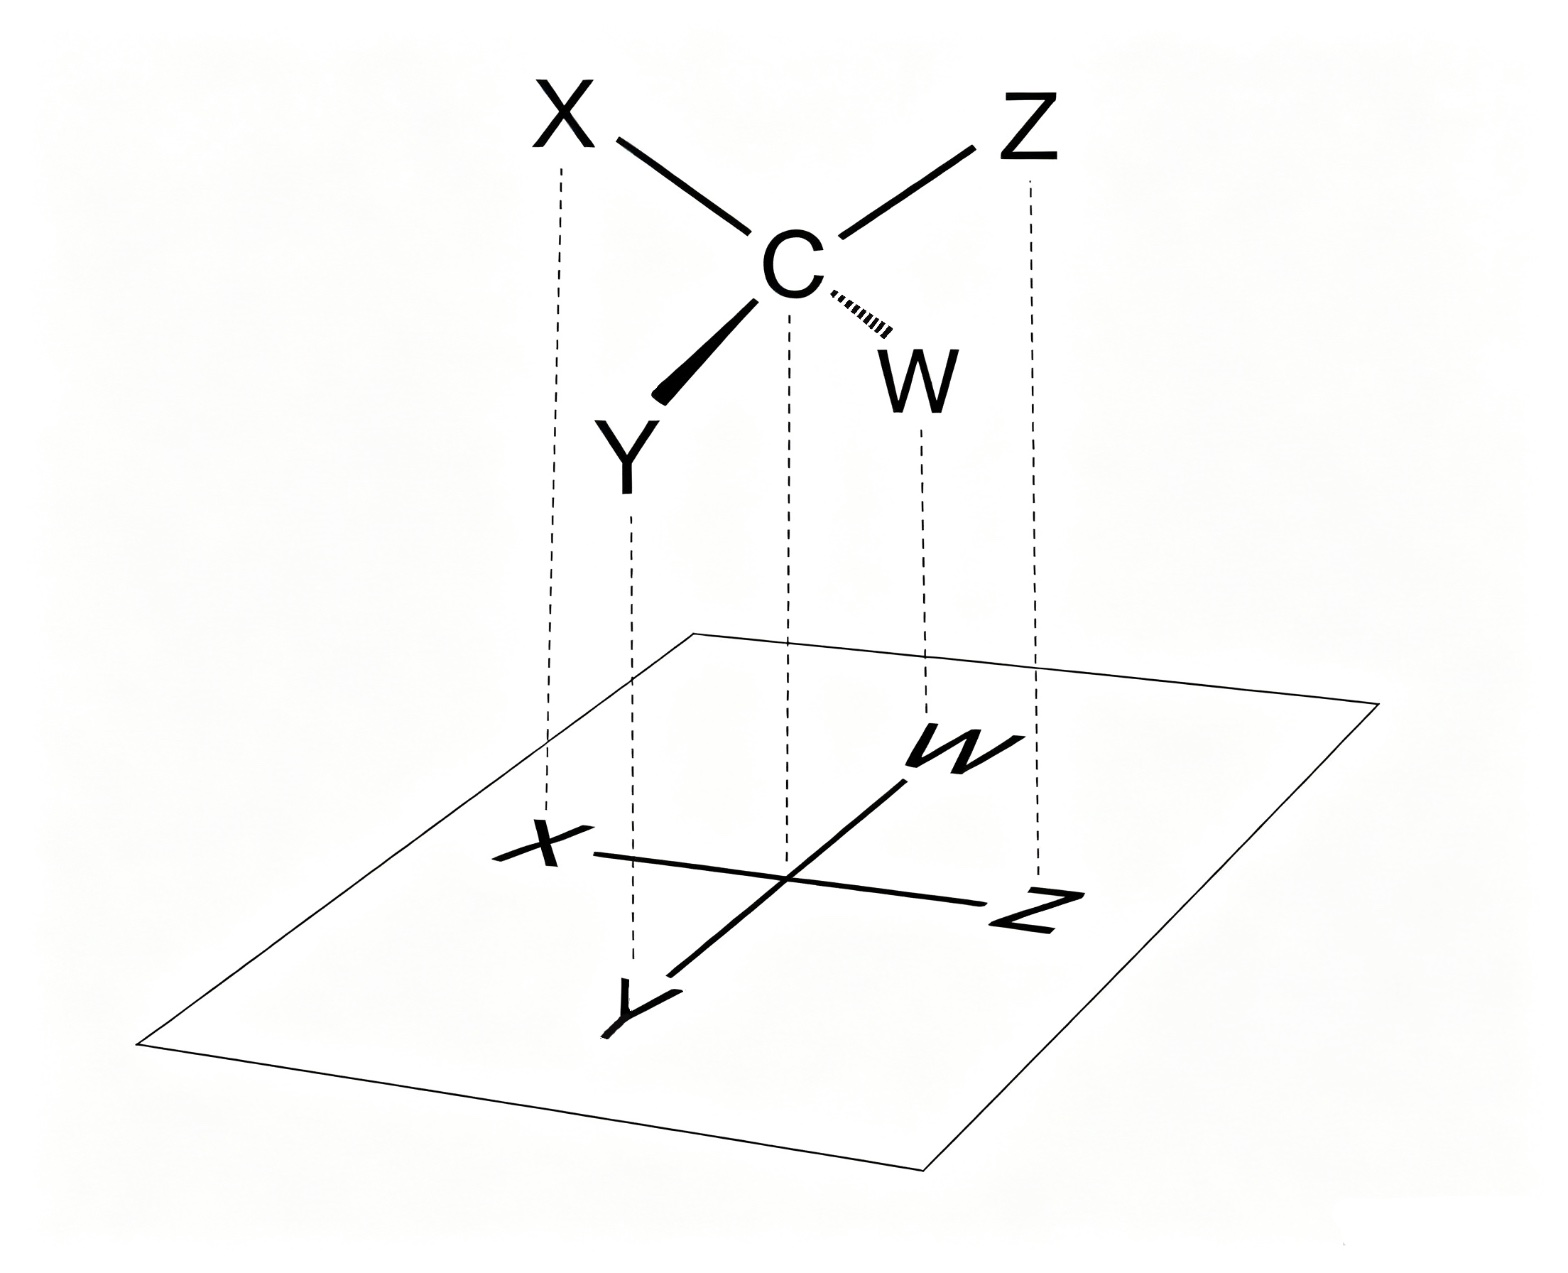
\includegraphics[width=0.5\textwidth]{20261103-fischer-projection.jpeg}
  \caption{Fischer 投影}
  \label{fig:fischer-projection}
\end{figure}
这个约定不是凭空规定的，而是把四面体“压平”的必然结果。如图~\ref{fig:fischer-projection}，$X$、$Z$ 在纸面内，$Y$ 用实楔伸出纸面，$W$ 用虚楔伸向纸面背后。沿观察方向把四个基团垂直投影到后面的投影面上，$X$、$Z$ 变成水平的左右两键，$Y$、$W$ 变成竖直的上下两键——由于 $Y$ 本来朝向读者、$W$ 本来背离读者，投影后竖直键指向后方、水平键指向读者，这正是 Fischer 投影式的写法。

Fischer 投影式有两条操作规则：在纸面内旋转 $180^\circ$ 不改变构型；旋转 $90^\circ$ 或交换任意两个基团则构型翻转。这条规则在比较糖的构型、判断内消旋体时非常有用。

手性中心的构型用 R/S 标记。步骤是：按 CIP 规则给四个基团排优先级（原子序数大者优先，同位素重者优先，双键按“复制”处理）；把最低优先级基团转向背后；剩余三个基团从高到低若为顺时针，记 R，逆时针记 S。这里有一个野路子记法，就是书写R的时候是顺时针的，所以排序是顺时针的就是R，反之亦然。

\subsection{顺反异构}

双键的构型用 E/Z 标记。比较双键每一端两个基团的优先级，高优先级基团在异侧为 E（反），在同侧为 Z（顺）。当双键两端各有一个氢时，E/Z 与顺反是一致的；当两端都有两个非氢基团时，只能用 E/Z。

\begin{center}
反-2-丁烯：\chemfig{-[:30](-[2]H)=[:-30](-[-2]H)-[:30]}
\qquad
顺-2-丁烯：\chemfig{-[:30](-[2]H)=[:-30](-[-2])-[:30]H}
\end{center}

\subsection{环己烷：顺反、直立与平伏}

环己烷不是平面六边形，而是椅式构象。每个碳上有一根直立键（a 键，垂直于环的平均平面）和一根平伏键（e 键，大致沿环的外缘）。同一个碳上的 a 键与 e 键一上一下。

顺反异构与 R/S 的关系可以这样记：在 1,2-二取代环己烷中，顺式对应一个 a、一个 e，反式对应两个 a 或两个 e；在 1,3-二取代中，顺式对应两个 a 或两个 e，反式对应一 a 一 e；1,4-二取代则与 1,2 相反。与其背表，不如把椅式画出来，逐个数上下。

环己烷的椅式翻转会把所有 a 键变 e、e 键变 a，但不改变顺反关系。这一点在讨论取代环己烷的稳定性（大基团优先占 e 键）时是关键。


\newpage


% ---- chunk ch9_3 : 3.x 有机反应类型 ----


\section{有机反应机理}

基本上所有的有机反应都离不开电性分子，也就是如下的三类分子：
\begin{center}
\chemfig{-[:30]-[:-30]-[:30]^{+}}
\qquad
\chemfig{-[:30]-[:-30]-[:30]^{-}}
\qquad
\chemfig{-[:30]-[:-30]-[:30]^{•}}
\end{center}
这样的分子是极不稳定/活泼的，所以一般只在机理中作为反应中间体出现，这三个一次是碳正离子，碳负离子，自由基。

三种粒子的电子数不同，稳定性规律也不同：碳正离子缺电子，靠给电子基团与共轭稳定；碳负离子富电子，靠吸电子基团与共轭稳定；自由基居中，靠共轭与位阻稳定。后面反复用到的，就是这三条稳定性顺序。

对于这些电性离子，都有一个统一的特性：在高级碳上稳定，所以都会有重排倾向，只不过各有不同罢了。这里指出，碳正离子的重排是三种电性离子中最活跃的，为什么？那当然是因为电子流动性强，所以正电荷的分散更容易啊。重排的驱动力通常只有一个：生成更稳定的正离子或更稳定的键。一般而言高级碳的超共轭效应和$\pi$电子的共轭效应，都可以稳定这些电性离子。

看懂重排，关键不是记名字，而是找到那个“迁移的基团”和“缺电子的中心”。最基础的就是碳正离子的 1,2-迁移：碳正离子旁边如果有氢或烷基，可以带着一对电子迁移到正电荷中心，正电荷随之转移到原来的位置。迁移的优先顺序是：氢 $>$ 芳基 $>$ 三级烷基 $>$ 二级烷基 $>$ 一级烷基。因为迁移时过渡态带部分正电荷，能给电子的基团迁移得快。

\begin{center}
\schemestart
\chemfig{-[:30](=[:90]O)-[:-30]-[:30]}
\arrow{->[\ce{mCPBA}]}
\chemfig{-[:30](=[:90]O)-[:-30]O-[:30]-[:-30]}
\schemestop
\end{center}

\subsection{自由基反应}

自由基反应由引发、增长、终止三步构成。以甲烷的氯代为例，光照使 \ce{Cl_2} 均裂产生氯自由基，氯自由基夺取甲烷的氢生成甲基自由基，甲基自由基再与 \ce{Cl_2} 反应生成氯甲烷并再生氯自由基：

\begin{center}
\schemestart
\chemfig{CH_4}
\arrow{->[\ce{Cl_2}][$h\nu$]}
\chemfig{-[:30]Cl}
\schemestop
\end{center}

一般而言，我们认为引发步需要外界提供能量（光、热或过氧化物）；增长步是链的循环，每一步都消耗一个自由基又产生一个自由基；终止步是两个自由基结合，链就此中断。理解这三步，就能理解为什么自由基反应对光敏感、为什么加入阻聚剂可以抑制反应、为什么产物分布由各步的相对速率决定。

双键旁边的碳（烯丙位）与苯环旁边的碳（苄位）生成的自由基可以被 $\pi$ 体系共轭稳定，因此这些位置的 \ce{C-H} 键特别容易被夺取。NBS（\ce{N}-溴代丁二酰亚胺）在光照或过氧化物引发下提供低浓度的 \ce{Br_2}，使溴代停在烯丙位或苄位而不加成到双键上：

\begin{center}
\schemestart
\chemfig{-[:-30]=[:30]}
\arrow{->[\ce{NBS}][$h\nu$]}
\chemfig{Br-[:30]-[:-30]=[:30]}
\schemestop
\end{center}

\begin{center}
\schemestart
\chemfig{*6(-=(-)-=-=)}
\arrow{->[\ce{NBS}][$h\nu$]}
\chemfig{*6(-=(-Br)-=-=)}
\schemestop
\end{center}


\newpage


% ---- chunk ch9_4 : 3.x 不饱和键亲电加成 ----


\section{不饱和键的亲电加成：正离子机理}

烯烃的 $\pi$ 电子是富电子的，是个极活跃的基团，容易被亲电试剂进攻。加成的第一步总是亲电试剂与 $\pi$ 键作用，区别在于中间体是“开放”的碳正离子，还是“桥连”的鎓离子。不过值得说明的是，虽然我们说是“容易被亲电试剂进攻”，但是其实一般都是电子去进攻正电荷，这是显然的，因为电子是“电子云”，是弥散在空间中的，变形性相比正电荷更好。

\begin{center}
\begin{tikzpicture}[>=Stealth, line width=0.6pt]
  % 第一段：丙烯 + E+
  \coordinate (a1) at (0,0);
  \coordinate (a2) at (0.72,0.42);
  \coordinate (a3) at (1.44,0);
  \draw (a1) -- (a2);
  \draw (a2) -- (a3);
  \draw ($(a2)!0.045!90:(a3)$) -- ($(a3)!0.045!-90:(a2)$);
  \node[font=\small] at (1.86,0.21) {$+$};
  \node[font=\small,anchor=west] at (2.04,0.21) {$E^{+}$};
  \node[font=\footnotesize,anchor=north] at (1.10,-0.42) {丙烯 + $E^{+}$};

  \draw[->] (2.72,0.21) -- (3.42,0.21);

  % 第二段：π 络合物
  \coordinate (b1) at (3.90,0);
  \coordinate (b2) at (4.62,0.42);
  \coordinate (b3) at (5.34,0);
  \draw (b1) -- (b2);
  \draw (b2) -- (b3);
  \draw ($(b2)!0.045!90:(b3)$) -- ($(b3)!0.045!-90:(b2)$);
  \draw (4.98,0.32) -- (4.98,0.92);
  \node[font=\small] at (4.98,1.10) {$E^{+}$};
  \node[font=\footnotesize,anchor=north] at (4.62,-0.42) {$\pi$ 络合物};

  % 分叉箭头
  \draw[->] (5.52,0.28) .. controls (6.28,0.58) .. (7.38,1.30);
  \draw[->] (5.52,0.10) .. controls (6.28,-0.34) .. (7.52,-1.24);

  % 上支：碳正离子
  \draw (7.55,1.15) -- (8.00,1.45) -- (8.45,1.15);
  \node[font=\small] at (8.20,1.66) {$+$};
  \node[font=\footnotesize] at (8.00,2.00) {马氏加成：坍缩为碳正离子};

  % 下支：鎓离子
  \coordinate (t2) at (8.00,-1.00);
  \coordinate (l2) at (7.65,-1.45);
  \coordinate (r2) at (8.35,-1.45);
  \draw (l2) -- (r2);
  \draw (r2) -- (8.62,-1.90);
  \draw[dash pattern=on 3pt off 2pt] (t2) -- (l2);
  \draw[dash pattern=on 3pt off 2pt] (t2) -- (r2);
  \node[font=\small] at (8.00,-0.76) {$E^{+}$};
  \node[font=\footnotesize,anchor=north] at (8.00,-2.14) {形成鎓离子（桥连中间体）};
\end{tikzpicture}
\end{center}

一般而言，对于小的亲核试剂，络合物会迅速坍缩为碳正离子；而对于半径比较大的亲核试剂，比如$Br^+$，由于半径过于大，溴的孤对电子可以与相邻的碳正离子形成三中心两电子键，桥连结构比开放碳正离子更稳定，所以一般会形成鎓离子中间体，随后也会坍缩为碳正离子。

碳正离子的坍缩是十分有门道的，起初我们只是单纯的发现：亲核试剂会倾向于加到氢离子更多的碳上，这后来也被成为马氏规则，是马尔科夫尼科夫发现的经验性定理。半个世纪后，美国化学家罗伯特·S·马利肯在1939年研究紫外光谱和共轭分子时首次提出，马氏规则的本质是超共轭效应稳定碳正离子，他发现，随着烯烃上连接的烷基增多，其吸收光谱会发生红移，并将这一现象归因于超共轭作用。

超共轭是什么，简而言之，碳原子的$sp^3$杂化使得每个轨道都带有一定的$\pi$电子成分，所以说这些$sp^3$电子也可以起到$\pi$电子类似的共轭效应，从而通过给电子来分散正电荷。所以说马氏规则的本质不是氢的多少，而是碳的多少，碳上连的碳越多，可以产生超共轭效应的$sp^3$电子也就越多，所以连接碳越多的碳所形成的碳正离子更加稳定。

后来随着人们继续使用，衍生出了碳的等级，和碳所连的碳的个数正相关，连一个碳的碳是一级碳，连两个碳的是二级碳，以此类推。在中国我们更习惯用兄弟辈次的伯仲叔季。

所以说，马氏规则的本质不是“氢加在氢多的地方”，而是“正电荷落在更稳定的碳上”。

但是，我们却发现了异常，比如……反应的时候，居然出现了第三种产物。通过衍射发现，它的碳骨架居然改变了。瓦格纳提出，当骨架中存在更高级的碳的时候，其上的甲基/质子会发生迁移，使得正电荷最终落在最高级的碳上，这个发现被称为碳正离子的重排。

\subsection{烯烃}

\subsubsection{马氏规则反应工具}

非常质朴的，\ce{HX} 与烯烃加成，卤素与烯烃加成，都遵循马氏规则。

羟汞化-脱汞是更温和的替代：醋酸汞 \ce{Hg(OAc)_2} 与烯烃生成汞鎓离子，水进攻后再用 \ce{NaBH_4} 脱汞。它同样得到马氏产物，但中间体是环状的汞鎓离子，不发生重排。

\begin{center}
\schemestart
\chemfig{-[:30]=[:-30]}
\arrow{->[\ce{Hg(OAc)_2}, \ce{H_2O}][\ce{NaBH_4}]}
\chemfig{-[:30](-[2]OH)-[:-30]}
\schemestop
\end{center}

\subsubsection{反马氏规则反应工具}

\ce{HBr} 与烯烃加成时，若体系中存在过氧化物，产物由马氏变为反马氏。原因是过氧化物均裂产生的自由基引发了另一条链：溴自由基先加到双键末端，生成较稳定的仲碳自由基，再夺取 \ce{HBr} 的氢，得到末端溴代烷。

\begin{center}
\schemestart
\chemfig{-[:30]=[:-30]}
\arrow{->[\ce{HBr}][过氧化物]}
\chemfig{-[:30]-[:-30]-[:30]Br}
\schemestop
\end{center}
注意这条规则只对 \ce{HBr} 有效。\ce{HCl} 的键太强，\ce{HI} 的碘自由基太容易结合成 \ce{I_2}，两者都不发生有效的过氧化物效应。

硼烷（\ce{BH_3}，通常以 \ce{THF} 或 \ce{Me_2S} 的配合物形式使用）是一个缺电子试剂，硼上有一个空轨道。它与烯烃反应时，硼加到取代较少、位阻较小的碳上，氢加到取代较多的碳上——这与马氏规则相反。原因不是电子效应，而是位阻与电子效应的共同作用：硼原子较大，倾向于靠近位阻较小的端位碳；同时过渡态中硼与端位碳成键时，部分正电荷落在取代较多的碳上，可以被烷基稳定。两个因素同向，因此取向很干净。

\begin{center}
\schemestart
\chemfig{-[:30]=[:-30]}
\arrow{->[\ce{BH_3}][\ce{THF}]}
\chemfig{-[:30]-[:-30]-[:30]BH_2}
\arrow{->[\ce{H_2O_2}][\ce{NaOH}]}
\chemfig{-[:30]-[:-30]-[:30]OH}
\schemestop
\end{center}

一分子 \ce{BH_3} 可以依次与三分子烯烃反应，生成三烷基硼；实际合成中常使用位阻更大的硼烷（如 9-BBN、二异戊基硼烷）来提高选择性，或只让一分子烯烃加成后直接氧化。硼氢化-氧化常被用来做三件事：把末端烯烃变成伯醇（反马氏），把末端炔变成醛，以及在存在敏感官能团时做温和的水合。它与羟汞化-脱汞构成一对互补工具：需要马氏醇用后者，需要反马氏醇用前者。

\subsubsection{双键的氧化}

过氧酸（如 mCPBA）与烯烃反应，把一个氧原子协同地加到双键上，生成环氧化物。这是一个协同过程，氧的转移与双键的断裂同时发生，因此保持烯烃的立体化学（顺式烯烃得顺式环氧）。

\begin{center}
\schemestart
\chemfig{-[:30]=[:-30]}
\arrow{->[\ce{mCPBA}][\ce{CH_2Cl_2}]}
\chemfig{*3(O--(-)--)}
\schemestop
\end{center}

环氧化物是三元环，张力大，容易被亲核试剂开环。碱性条件下亲核试剂进攻取代较少的碳（\ce{S_N2}，位阻控制）；酸性条件下环氧先质子化，亲核试剂进攻取代较多的碳（正电荷更集中）。这一取向差异在合成中非常有用。

\begin{center}
\schemestart
\chemfig{*3(O--(-)--)}
\arrow{->[\ce{CH_3O^-}][甲醇]}
\chemfig{-[:30](-[2]OH)-[:-30]-[:30]O-[:-30]}
\schemestop
\end{center}

四氧化锇或冷的高锰酸钾把烯烃氧化成邻二醇，两个羟基从同一面加上（顺式加成）。\ce{OsO_4} 毒性大、价格高，通常用催化量并配 \ce{NMO} 等再生氧化剂。

\begin{center}
\schemestart
\chemfig{-[:30]=[:-30]-[:30]}
\arrow{->[\ce{OsO_4}][\ce{NMO}, \ce{H_2O}]}
\chemfig{-[:30](-[2]OH)-[:-30](-[-2]OH)-[:30]}
\schemestop
\end{center}

臭氧分解是切断双键的经典方法。臭氧先与双键发生环加成，生成臭氧化物，随后重排、分解。还原性后处理（\ce{Zn/H_2O} 或 \ce{Me_2S}）得到醛或酮；氧化性后处理（\ce{H_2O_2}）得到羧酸。这个反应可以用来定位双键的位置。

\begin{center}
\schemestart
\chemfig{-[:30]=[:-30]-[:30]-[:-30]}
\arrow{->[1.\ \ce{O_3}][2.\ \ce{Zn}, \ce{H_2O}]}
\chemfig{-[:30](=[:90]O)-[:-30]H}
\+
\chemfig{-[:30]-[:-30](=[-2]O)-[:30]H}
\schemestop
\end{center}

\subsubsection{不饱和键的还原}

氢气在金属表面（\ce{Pd}、\ce{Pt}、\ce{Ni}）上解离成氢原子，两个氢原子从同一面加到双键上，因此是顺式加成。炔烃部分氢化可以用 Lindlar 催化剂（毒化的钯）停在顺式烯烃；用钠/液氨则得到反式烯烃。

\begin{center}
\schemestart
\chemfig{-[:30]~[:30]-[:30]}
\arrow{->[\ce{H_2}][Lindlar]}
\chemfig{-[:30]=[:-30]-[:30]}
\schemestop
\end{center}

\subsection{炔烃}

末端炔的 \ce{C-H} 具有弱酸性（pKa 约 25），可以被强碱（\ce{NaNH_2}、\ce{n-BuLi}）夺取，生成炔钠。炔钠是亲核试剂，与伯卤代烷发生 \ce{S_N2}，是延长碳链的常用手段。

\begin{center}
\schemestart
\chemfig{-[:30]~[:30]H}
\arrow{->[1.\ \ce{NaNH_2}, 液氨][2.\ \ce{CH_3CH_2Br}]}
\chemfig{-[:30]~[:30]-[:30]-[:-30]}
\schemestop
\end{center}

炔烃的亲电加成可以停在一分子，得到烯烃；由于中间体乙烯基正离子不如烷基正离子稳定，加成速率比烯烃慢，取向也更复杂。炔烃水合（\ce{HgSO_4/H_2SO_4}）遵循马氏规则，生成烯醇后互变异构为酮；末端炔生成甲基酮。

末端炔硼氢化后氧化，得到烯醇，烯醇互变异构为醛；内炔则得到酮。这与炔烃水合的马氏取向正好互补：

\begin{center}
\schemestart
\chemfig{-[:30]-[:-30]~[:-30]H}
\arrow{->[1.\ \ce{BH_3}][2.\ \ce{H_2O_2}, \ce{OH^-}]}
\chemfig{-[:30]-[:-30]-[:30](=[:90]O)-[:-30]H}
\schemestop
\end{center}


\subsection{共轭二烯与 Diels--Alder 反应}

共轭二烯的亲电加成有两个产物：1,2-加成与 1,4-加成。前者是动力学产物（低温有利），后者是热力学产物（高温有利），因为 1,4-产物的双键取代更多、更稳定。

\begin{center}
\schemestart
\chemfig{=[:30]-[:-30]=[:30]}
\arrow{->[\ce{HBr}][低温]}
\chemfig{-[:30](-[2]Br)-[:-30]=[:30]}
\schemestop
\qquad
\schemestart
\chemfig{=[:30]-[:-30]=[:30]}
\arrow{->[\ce{HBr}][高温]}
\chemfig{Br-[:30]-[:-30]=[:30]}
\schemestop
\end{center}

Diels--Alder 反应是共轭二烯与亲双烯体之间的 [4+2] 环加成。它是一步协同反应，没有中间体，因此具有高度的立体专一性：顺式亲双烯体给出顺式产物，二烯的 \emph{s-cis} 构象决定环的尺寸。内型产物（endo）通常动力学有利，因为次级轨道作用更稳定。

\begin{center}
\schemestart
\chemfig{=[:30]-[:-30]=[:30]}
\arrow{->[$\Delta$]}
\chemfig{*6(---=--)}
\schemestop
\end{center}

上式的亲双烯体是乙烯，实际反应需要更活泼的亲双烯体（如马来酸酐、丙烯醛）。Diels--Alder 是构建六元环最可靠的方法，在天然产物合成中地位极高。


硼氢化是本章最值得单独讲的一类反应。它的价值在于三点：取向是反马氏，立体化学是顺式，条件温和且不重排。这三点正好补上了酸催化水合与羟汞化的短板。

\newpage


% ---- chunk ch9_5 : 3.x 取代与消除 ----


\section{取代与消去}

同一底物在不同条件下可以得到取代或消除产物。经验规律是：强亲核弱碱（如 \ce{I^-}、\ce{CN^-}）利于取代；强碱大位阻（如 \ce{t-BuO^-}）利于消除；高温利于消除（熵增）；叔底物利于 \ce{S_N1}/E1，伯底物利于 \ce{S_N2}。

\begin{center}
\begin{tabular}{lll}
\toprule
底物 & 强亲核弱碱 & 强碱大位阻 \\
\midrule
伯卤代烷 & \ce{S_N2} & E2（少） \\
仲卤代烷 & \ce{S_N2} 与 E2 竞争 & E2 \\
叔卤代烷 & \ce{S_N1} 与 E1 竞争 & E2（少，主要为 E1） \\
\bottomrule
\end{tabular}
\end{center}

亲核取代是有机化学中最基本的反应之一：一个亲核试剂进攻带有离去基团的碳，取代离去基团。按机理分为 \ce{S_N2}（一步协同）与 \ce{S_N1}（分步，经碳正离子）。



\subsection{$S_N1$：碳正离子与消旋}

E1 与 \ce{S_N1} 共享碳正离子中间体：先离解，再失去 $\beta$-氢。它通常伴随 \ce{S_N1} 取代产物，且由于碳正离子可重排，产物可能异构化。

E1cb 是“共轭碱消除”：$\beta$-氢先被碱夺取，生成碳负离子（烯醇负离子），然后离去基团离开。它常见于 $\beta$-卤代羰基化合物、$\beta$-羟基羰基化合物，因为生成的碳负离子可以被羰基稳定。

叔卤代烷在极性溶剂中先离解成碳正离子，再被亲核试剂捕获。由于碳正离子是平面结构，两侧都可以进攻，产物通常消旋；若碳正离子可以重排，还会得到重排产物。

\begin{center}
\schemestart
\chemfig{-[:30](-[2])(-[:150]Br)-[:-30]}
\arrow{->[\ce{H_2O}]}
\chemfig{-[:30](-[2])(-[:150]OH)-[:-30]}
\schemestop
\end{center}

\ce{S_N1} 的速率只与底物浓度有关（一级），因为离解是决速步。溶剂的极性、离去基团的好坏、碳正离子的稳定性决定速率；亲核试剂的强弱影响不大。

\subsection{$S_N2$：手性反转}


E2 是协同反应，碱夺取 $\beta$-氢的同时离去基团离开，形成双键。它要求 \ce{C-H} 与 \ce{C-X} 处于反式共平面（anti-periplanar），这样两个正在断裂的键的电子云才能最大程度重叠。

在环己烷体系中，反式共平面意味着离去基团与 $\beta$-氢必须都是直立键（trans-diaxial）。因此环己烷的 E2 消除有严格的立体要求：只有处于反式二直立位置的氢才能被消除。

\begin{center}
\schemestart
\chemfig{*6(-(-Br)-----)}
\arrow{->[\ce{CH_3CH_2O^-}]}
\chemfig{*6(---=--)}
\schemestop
\end{center}


小碱（如乙醇钠）夺取取代较多的 $\beta$-氢，生成取代较多的烯烃，这是 Zaitsev 规则（热力学更稳定的烯烃为主）。大位阻碱（如叔丁醇钾）夺取位阻较小的 $\beta$-氢，生成末端烯烃，这是 Hofmann 规则。

\begin{center}
\schemestart
\chemfig{-[:30]-[:-30](-[-2]Br)-[:30]}
\arrow{->[\ce{EtO^-}]}
\chemfig{-[:30]=[:-30]-[:30]}
\schemestop
\qquad
\schemestart
\chemfig{-[:30]-[:-30](-[-2]Br)-[:30]}
\arrow{->[\ce{t-BuO^-}]}
\chemfig{-[:30]-[:-30]=[:30]}
\schemestop
\end{center}


\ce{S_N2} 的过渡态是五配位，亲核试剂从离去基团的背面进攻，三个非反应基团在过渡态中近似共平面。结果是构型翻转（Walden 翻转），就像雨伞被风吹翻。

\begin{center}
\schemestart
\chemfig{-[:30]-[:-30]Br}
\arrow{->[\ce{OH^-}][\ce{H_2O}]}
\chemfig{-[:30]-[:-30]OH}
\schemestop
\end{center}

\ce{S_N2} 的速率由底物浓度与亲核试剂浓度共同决定（二级）。影响速率的因素包括：底物的位阻（甲基 $>$ 伯 $>$ 仲 $\gg$ 叔）、亲核试剂的强弱、离去基团的好坏（\ce{I^-} $>$ \ce{Br^-} $>$ \ce{Cl^-} $>$ \ce{F^-}）、溶剂的极性（极性非质子溶剂最好）。

季铵盐在氧化银作用下加热，发生 E2 消除，生成取代最少的烯烃（Hofmann 产物）。原因是季铵基 \ce{-N^+R_3} 是很好的离去基团，反应更接近 E1cb，碱性的差异与位阻共同决定了取向。这个反应在生物碱结构测定中曾用来确定氮的位置。

\subsection{烷氧基的活化}

醇本身不是好的离去基团（\ce{OH^-} 是强碱），需要先质子化或转化为更好的离去基团。常用试剂有 \ce{HX}、\ce{PBr_3}、\ce{SOCl_2}、\ce{TsCl}。

\ce{PBr_3} 与醇反应，经亚磷酸酯中间体，溴从背面进攻，构型翻转。\ce{SOCl_2} 与醇反应，经氯代亚硫酸酯，通常构型保持（\ce{S_Ni} 机理），但加入吡啶时也可能翻转。选择试剂时要把立体化学一并考虑。

\begin{center}
\schemestart
\chemfig{-[:30]-[:-30]OH}
\arrow{->[\ce{SOCl_2}][吡啶]}
\chemfig{-[:30]-[:-30]Cl}
\schemestop
\end{center}

Williamson 醚合成是醇钠（或酚钠）与伯卤代烷的 \ce{S_N2} 反应。由于是 \ce{S_N2}，卤代烷必须是伯或甲基，否则消除产物会占主导。

\begin{center}
\schemestart
\chemfig{-[:30]-[:-30]O^{\ominus}}
\arrow{->[\ce{CH_3CH_2Br}]}
\chemfig{-[:30]-[:-30]O-[:30]-[:-30]}
\schemestop
\end{center}

醚的断裂用浓 \ce{HI} 或 \ce{HBr}：醚先质子化，卤离子进攻位阻较小的碳，生成醇与卤代烷。芳基烷基醚断裂时，进攻发生在烷基一侧，因为芳基碳不能发生 \ce{S_N2}。

醇在酸催化下脱水，机理是质子化羟基、离解成碳正离子、失去 $\beta$-氢。与 \ce{S_N1} 一样，碳正离子会重排，因此新戊醇脱水得到重排产物而不是末端烯烃。

\begin{center}
\schemestart
\chemfig{-[:30]-[:-30]OH}
\arrow{->[\ce{H_2SO_4}][$170\,^{\circ}\mathrm{C}$]}
\chemfig{=[:30]}
\schemestop
\end{center}





\newpage


% ---- chunk ch9_6 : 3.x 芳香亲电取代 ----


\section{芳烃的亲电取代}

苯环的 $\pi$ 电子同样是富电子的，但苯不与溴水加成，也不与高锰酸钾反应。原因在于芳香性：六个 $\pi$ 电子离域在环上，整体能量很低，加成会破坏这个离域体系。因此芳烃的典型反应不是加成，而是取代——用一个亲电试剂替换环上的氢，芳香性得以保留。

\subsection{$\sigma$ 络合物：取代反应的中枢}

亲电取代的第一步是亲电试剂进攻环，形成一个带正电荷的环己二烯基正离子，称为 $\sigma$ 络合物（也称芳基正离子）。正电荷离域在环的五个碳上，芳香性暂时被破坏。第二步是失去质子，恢复芳香性。

\begin{center}
\schemestart
\chemfig{*6(=-=-=-)}
\arrow{->[\ce{E^+}]}
\chemfig{*6(-=(-E)-=-=)}
\schemestop
\end{center}

这个两步机理解释了两件事。第一，取代反应需要“强亲电试剂”，因为要破坏芳香性，代价高；第二，凡能使 $\sigma$ 络合物更稳定的因素都会加速反应，这正是后面定位效应的根源。

\subsection{四类基本反应}

硝化用浓硝酸与浓硫酸的混酸，真正的亲电试剂是硝酰正离子 \ce{NO_2^+}：

\begin{center}
\schemestart
\chemfig{*6(=-=-=-)}
\arrow{->[\ce{HNO_3}, \ce{H_2SO_4}][$50\,^{\circ}\mathrm{C}$]}
\chemfig{*6(-=(-NO_2)-=-=)}
\schemestop
\end{center}

磺化用发烟硫酸或浓硫酸，亲电试剂是 \ce{SO_3}。磺化是可逆的，把磺酸基放在稀酸中加热可以脱去，这一性质常被用作“占位基”：先占住某个位置，反应完再脱掉。

\begin{center}
\schemestart
\chemfig{*6(=-=-=-)}
\arrow{->[\ce{SO_3}][\ce{H_2SO_4}]}
\chemfig{*6(-=(-SO_3H)-=-=)}
\schemestop
\end{center}

卤代需要路易斯酸活化，溴本身亲电性不够，与 \ce{FeBr_3} 生成更强的亲电试剂：

\begin{center}
\schemestart
\chemfig{*6(=-=-=-)}
\arrow{->[\ce{Br_2}][\ce{FeBr_3}]}
\chemfig{*6(-=(-Br)-=-=)}
\schemestop
\end{center}

Friedel--Crafts 反应分烷基化与酰化两种。烷基化用卤代烷加 \ce{AlCl_3}，本质是碳正离子进攻芳环：

\begin{center}
\schemestart
\chemfig{*6(=-=-=-)}
\arrow{->[\ce{CH_3CH_2Cl}][\ce{AlCl_3}]}
\chemfig{*6(-=(--[:30])-=-=)}
\schemestop
\end{center}

烷基化有三个毛病：碳正离子会重排（正丙基氯给出异丙苯）；产物比原料更活泼，容易多烷基化；强酸条件下氨基会成盐而钝化环。酰化没有这些问题：酰基正离子不重排，产物酮被钝化因而停在单取代，且不会发生多酰化。

\begin{center}
\schemestart
\chemfig{*6(=-=-=-)}
\arrow{->[\ce{CH_3COCl}][\ce{AlCl_3}]}
\chemfig{*6(-=(-(=[::60]O)-[::-60])-=-=)}
\schemestop
\end{center}

酰化的产物可以进一步还原成烷基（Clemmensen 还原用锌汞齐/盐酸，Wolff--Kishner 还原用水合肼/碱），因此“先酰化再还原”是制备直链烷基苯的标准路线，可以绕开重排。

\subsection{定位效应：谁决定第二个基团的位置}

环上已有取代基时，第二个亲电试剂进入的位置由该取代基决定。规律分两类：

\begin{center}
\begin{tabular}{lll}
\toprule
取代基类型 & 例子 & 进入位置 \\
\midrule
致活、邻对位 & \ce{-OH}、\ce{-OR}、\ce{-NH_2}、烷基 & 邻位与对位 \\
致钝、邻对位 & 卤素 & 邻位与对位 \\
致钝、间位 & \ce{-NO_2}、\ce{-CN}、\ce{-COOH}、\ce{-SO_3H} & 间位 \\
\bottomrule
\end{tabular}
\end{center}

解释要看 $\sigma$ 络合物的稳定性。以甲苯为例，甲基通过超共轭与诱导给电子，稳定正电荷；当亲电试剂进入邻位或对位时，正电荷正好落在带甲基的碳上或其邻位，可以被甲基稳定。间位进攻时正电荷不落在该碳上，得不到这份稳定化，因此邻对位产物占优。

\begin{center}
\schemestart
\chemfig{*6(-=(-)-=-=)}
\arrow{->[\ce{HNO_3}, \ce{H_2SO_4}]}
\chemfig{*6(-=(-)-(-NO_2)=-=)}
\schemestop
\end{center}

硝基苯的情况相反：硝基强吸电子，邻对位进攻时正电荷会落到带硝基的碳上，被进一步抽走电子，$\sigma$ 络合物特别不稳定；间位进攻避开了这一点，所以主要得到间位产物。

\begin{center}
\schemestart
\chemfig{*6(-=(-NO_2)-=-=)}
\arrow{->[\ce{HNO_3}, \ce{H_2SO_4}]}
\chemfig{*6(-=(-NO_2)-=(-NO_2)-=)}
\schemestop
\end{center}

卤素是“致钝但邻对位”的例外：卤素的诱导效应吸电子（使环钝化），但孤对电子可以共轭给电子（稳定邻对位的 $\sigma$ 络合物）。诱导决定速率，共轭决定位置，两者方向不同，于是出现这种组合。

更深一层的原因是轨道匹配。O、N 是第二周期元素，$2p$ 轨道与苯环碳的 $2p$ 轨道尺寸相近，$p$-$\pi$ 共轭有效，所以 \ce{-OH}、\ce{-NH_2} 是致活基；Cl、Br、I 在第三周期以后，$p$ 轨道弥散，与 $2p$ 的重叠变差，共轭减弱，电负性诱导效应就占了上风，于是表现为钝化。同一族从上到下（\ce{F} 到 \ce{I}），共轭越来越弱、钝化越来越强，这条趋势正是“轨道匹配 + 电性效应”的直接推论。

当环上有两个取代基时，定位能力强的优先。一般的强弱顺序是：\ce{-NH_2}、\ce{-OH} $>$ \ce{-OR} $>$ 烷基 $>$ 卤素 $>$ 间位定位基。若两个基团方向冲突，以强者为准；若两者都强且互为对位，往往得到混合物。

\subsection{萘与多环芳烃}

萘可以看作两个苯环并合，它的亲电取代优先发生在 $\alpha$ 位（1 位），因为 $\alpha$ 位进攻形成的 $\sigma$ 络合物可以保留另一个环的完整芳香性，共振式更多、更稳定。萘的磺化有温度依赖：低温得 $\alpha$-萘磺酸（动力学），高温得 $\beta$-萘磺酸（热力学，位阻小）。

蒽与菲的反应性更高，但氧化也更容易，合成上常需要保护。多环芳烃的致癌性与代谢中生成的环氧化物有关，这是“结构决定性质”的一个著名例子。

\subsection{侧链反应}

芳环侧链的苄位氢容易被自由基夺取（前面 NBS 一节已见），也容易被氧化。用高锰酸钾或重铬酸钾加热，只要苄位有氢，侧链就一路氧化到羧基：

\begin{center}
\schemestart
\chemfig{*6(-=(--[:30])-=-=)}
\arrow{->[\ce{KMnO_4}, \ce{H^+}][$\Delta$]}
\chemfig{*6(-=(-(=[::60]O)-[::-60]OH)-=-=)}
\schemestop
\end{center}

苄位没有氢（如叔丁基苯）则不反应。这条规律既可以用来制备芳香羧酸，也可以用来判断侧链结构。

\subsection{芳环上的亲核取代与苯炔}

芳环通常不被亲核试剂进攻，但有两个例外。其一，环上有强吸电子基（尤其是邻对位的硝基）时，可以发生加成-消除型的 \ce{S_NAr}：亲核试剂先加成形成 Meisenheimer 络合物，再消除卤离子。硝基的作用是稳定负电荷。

其二，在强碱（如 \ce{NaNH_2}/液氨）下，卤代苯先消除 \ce{HX} 生成苯炔，苯炔再被亲核试剂加成，得到取代产物：

\begin{center}
\schemestart
\chemfig{*6(-=(-Cl)-=-=)}
\arrow{->[\ce{NaNH_2}][液氨]}
\chemfig{*6(-=(-NH_2)-=-=)}
\schemestop
\end{center}

苯炔中间体解释了“ cine 取代”：若卤素邻位有取代基，产物是混合物，因为亲核试剂可以从三键的两端进攻。这个机理是芳环上“看似不可能”的取代反应的钥匙。

\newpage


% ---- chunk ch9_7 : 3.x 羰基化学 ----


\section{羰基化学}

羰基是有机化学的中心。碳氧双键强极化，碳带部分正电荷，几乎所有的亲核试剂都盯着这个碳。羰基化学的骨架只有一句话：亲核试剂加到碳上，$\pi$ 键打开，氧带负电，随后质子化。

\subsection{亲核加成的活性顺序}

醛比酮活泼，因为烷基的给电子与位阻都不利于进攻。脂肪醛 $>$ 芳香醛 $>$ 酮 $>$ 酯 $>$ 酰胺，这个顺序既是电子效应也是位阻的结果，后面判断“谁能被谁还原”时反复用到。

\subsection{氰醇、亚胺与缩醛}

醛酮与 \ce{HCN} 加成生成 $\alpha$-羟基氰（氰醇）。这个中间体是增碳的跳板：酸性水解得 $\alpha$-羟基酸 $\mathrm{R_2C(OH)COOH}$，\ce{LiAlH_4} 还原得 $\beta$-氨基醇 $\mathrm{R_2C(OH)CH_2NH_2}$。氰醇化可逆，碱性条件下易解离回醛酮，通常现配现用。

\begin{center}
\schemestart
\chemfig{-[:30](=[:90]O)-[:-30]H}
\arrow{->[\ce{HCN}]}
\chemfig{-[:30](-[2]OH)-[:-30]C~N}
\schemestop
\end{center}

与氨或伯胺反应，先加成再脱水，生成亚胺（Schiff 碱）。亚胺的 \ce{C=N} 键也可以被亲核试剂进攻，而且比羰基更容易被还原（还原胺化）：

\begin{center}
\schemestart
\chemfig{-[:30](=[:90]O)-[:-30]H}
\arrow{->[\ce{RNH_2}][$-\ce{H_2O}$]}
\chemfig{-[:30]=[:-30]N-R}
\schemestop
\end{center}

与醇在酸催化下反应，生成缩醛（酮则生成缩酮）。缩醛对碱与亲核试剂稳定，只在酸性水溶液中水解，因此是羰基最常用的保护基。合成上常把醛变成缩醛，做完对碱敏感的反应后再水解复原。

\begin{center}
\schemestart
\chemfig{-[:30](=[:90]O)-[:-30]H}
\arrow{->[\ce{2 EtOH}][\ce{H^+}]}
\chemfig{-[:30](-[2]O-[:30]-[:-30])(-[:-30]O-[:30]-[:-30])}
\schemestop
\end{center}

仲胺与醛酮反应则生成烯胺：先成亚胺，再失去 $\alpha$-氢，双键移到 $\alpha$ 位。烯胺是烯醇负离子的“稳定版本”，可以做亲核试剂，这是 Stork 烯胺合成的基础。

\subsection{格氏试剂与氢化物}

格氏试剂（\ce{RMgX}）与醛酮加成，是构建碳碳键最直接的方法。甲醛给出伯醇，其他醛给出仲醇，酮给出叔醇：

\begin{center}
\schemestart
\chemfig{-[:30](=[:90]O)-[:-30]H}
\arrow{->[1.\ \ce{CH_3MgBr}][2.\ \ce{H_3O^+}]}
\chemfig{-[:30](-[2]OH)-[:-30]}
\schemestop
\end{center}

格氏试剂有两怕：水（会淬灭）和活泼氢（醇、胺、羧酸都行）。因此反应必须在无水醚类溶剂中进行，原料中不能带活泼氢。

氢化物（\ce{LiAlH_4}、\ce{NaBH_4}）把羰基还原成醇。\ce{LiAlH_4} 更强，能还原羧酸、酯、酰胺；\ce{NaBH_4} 温和，只还原醛酮。这个差别在选择性还原中很有用。

\subsection{$\alpha$-氢的酸性：烯醇与烯醇负离子}

羰基旁边的 $\alpha$-氢有酸性，因为失去质子后生成的烯醇负离子可以被羰基共轭稳定。pKa 约为 20（酮）到 25（酯），比普通烷烃氢（pKa 50）强得多，但仍弱于醇（16）。因此制备烯醇负离子要用更强的碱（LDA），而乙醇钠只能建立平衡。

烯醇负离子是两可亲核试剂：可以进攻羰基碳（C-烷基化），也可以进攻卤代烷（C-烷基化）或氧（O-烷基化）。用 LDA 在低温下生成动力学控制的烯醇负离子，再用活泼卤代烷捕获，是定向烷基化的标准做法。

\subsection{羟醛缩合}

两分子醛在碱催化下缩合：一分子生成烯醇负离子，进攻另一分子的羰基，得到 $\beta$-羟基醛（羟醛）；加热则脱水生成 $\alpha,\beta$-不饱和醛。

\begin{center}
\schemestart
\chemfig{-[:30](=[:90]O)-[:-30]H}
\arrow{->[\ce{OH^-}]}
\chemfig{-[:30](-[2]OH)-[:-30]-[:30](=[:90]O)-[:-30]H}
\arrow{->[$\Delta$][$-\ce{H_2O}$]}
\chemfig{-[:30]=[:-30]-[:30](=[:90]O)-[:-30]H}
\schemestop
\end{center}

交叉羟醛缩合若两种醛都有 $\alpha$-氢，会得到四种产物，没有合成价值。解决办法是让一种醛没有 $\alpha$-氢（如苯甲醛、甲醛），它只能做亲电体，缩合就变得干净。

\subsection{卤仿反应}

甲基酮（\ce{CH_3-CO-R}）与卤素在碱中反应，三个 $\alpha$-氢被卤代，随后碳碳键断裂，生成卤仿与羧酸盐。碘仿反应（\ce{I_2}/\ce{NaOH}）生成黄色的碘仿沉淀，是检验甲基酮与乙醛的经典方法，也是乙醇、异丙醇被误检的原因——它们先被氧化成乙醛或丙酮。

\begin{center}
\schemestart
\chemfig{-[:30](=[:90]O)-[:-30]}
\arrow{->[\ce{I_2}, \ce{NaOH}]}
\chemfig{CHI_3} + \chemfig{-[:30](=[:90]O)-[:-30]O^{\ominus}}
\schemestop
\end{center}

\subsection{羧酸衍生物：活性顺序与相互转化}

酰卤、酸酐、酯、酰胺的活性依次下降，因为离去基团越来越差（\ce{Cl^-} $>$ \ce{RCOO^-} $>$ \ce{RO^-} $>$ \ce{NH_2^-}）。高活性的可以转成低活性的，反之则需要活化。这条“活性阶梯”决定了合成路线：要制酰胺，就用酰氯与胺反应；要制酯，可以用酰氯或酸酐，也可以用酸加醇在酸催化下酯化。

\begin{center}
\schemestart
\chemfig{-[:30](=[:90]O)-[:-30]Cl}
\arrow{->[\ce{CH_3CH_2OH}][吡啶]}
\chemfig{-[:30](=[:90]O)-[:-30]O-[:30]-[:-30]}
\schemestop
\end{center}

酯的水解在酸或碱中进行。碱水解不可逆（生成的羧酸盐不再被醇进攻），因此皂化能进行到底；酸水解是可逆的，需要过量水推动。

\subsection{$\beta$-二羰基化合物：合成上的万能积木}

乙酰乙酸乙酯与丙二酸二乙酯的 $\alpha$-氢夹在两个羰基之间，酸性更强（pKa 约 11），可以被乙醇钠定量地夺去。生成的烯醇负离子与卤代烷烷基化，再水解脱羧，就得到取代的酮或羧酸。

\begin{center}
\schemestart
\chemfig{-[:30](=[:90]O)-[:-30]-[:30](=[:90]O)-[:-30]O-[:30]-[:-30]}
\arrow{->[1.\ \ce{EtO^-}][2.\ \ce{RX}]}
\chemfig{-[:30](=[:90]O)-[:-30](-[-2]R)-[:30](=[:90]O)-[:-30]O-[:30]-[:-30]}
\schemestop
\end{center}

乙酰乙酸酯合成给出取代丙酮，丙二酸酯合成给出取代乙酸。两者的共同点是：用一个容易引入、容易去掉的“活化基团”临时提高 $\alpha$ 位的反应性，用完后脱羧移除。这是有机合成里“临时官能团”思想的最早范例。

\subsection{Claisen 缩合与 Michael 加成}

两个酯在强碱下缩合，生成 $\beta$-酮酸酯，这是 Claisen 缩合。分子内的版本（Dieckmann 缩合）可以关环，是构建五元、六元环的常用手段。交叉 Claisen 缩合中，若一个酯没有 $\alpha$-氢（如草酸二乙酯、甲酸乙酯），反应就变得定向。

Michael 加成是烯醇负离子对 $\alpha,\beta$-不饱和羰基的共轭加成：负电荷加到 $\beta$ 位，双键移到 $\alpha$ 与羰基之间，最终在 $\beta$ 位形成新键。它与 1,2-加成（直接进攻羰基碳）竞争，用软亲核试剂（如烯醇负离子、硫醇）时 1,4-加成占优。

把 Michael 加成与羟醛缩合串起来，就是 Robinson 环化：先共轭加成，再分子内羟醛缩合，一步构建六元环。这是甾体合成的经典入口。



\newpage



% ---- combo ch4_1 + ch10[4.2:] : 第四章：ch4_1（2026-11-06 19:59 最新改写的章首+4.1 人名反应）拼接 ch10 的 4.2 之后各节 ----

\section{从反应到合成：人名反应、保护基与逆合成}

下面按反应类型汇总《基础有机化学》（第 4 版）上册各章涉及的常用反应。每条反应以键线式画出反应物，向右分出多条箭头，每条箭头标出条件、指向对应产物，反应名紧随产物之后。同一条件下若有两种产物（如 1,2- 与 1,4-加成），一并写在箭头末端。实际使用时需按底物与保护基情况调整。

% SKELETAL-BEGIN
{\small
\setchemfig{atom sep=1.9em,bond offset=1pt,cram width=1.2ex}
\par\nopagebreak[4]\addvspace{7pt}\noindent\textbf{自由基取代（第四章）}\par\nopagebreak[4]\addvspace{2pt}
\noindent\begin{tikzpicture}[baseline=0pt,x=1cm,y=1cm,font=\scriptsize]
\node[anchor=west,inner sep=1pt] (a) at (0,0) {\chemfig[baseline=(current bounding box.center)]{R-H}};
\draw[->] (a.east) -- (6.40,0) node[pos=0.5,above,font=\tiny,fill=white,inner sep=1pt,yshift=2pt]{$\mathrm{X_2}$，$h\nu$ 或 $\Delta$};
\node[anchor=west,inner sep=1pt] at (6.50,0) {\chemfig[baseline=(current bounding box.center)]{R-X}+\ce{HX}\ （卤代）};
\end{tikzpicture}\par\addvspace{3pt}

\par\nopagebreak[4]\addvspace{7pt}\noindent\textbf{亲核取代与消除（第六章）}\par\nopagebreak[4]\addvspace{2pt}
\noindent\begin{tikzpicture}[baseline=0pt,x=1cm,y=1cm,font=\scriptsize]
\node[anchor=west,inner sep=1pt] (a) at (0,0) {\chemfig[baseline=(current bounding box.center)]{R-X}};
\draw (a.east) -- ++(0.45,0) coordinate (t);
\draw ([yshift=3.00cm]t) -- ([yshift=-3.00cm]t);
\draw[->] (t) ++(0,3.00) -- (6.40,3.00) node[pos=0.5,above,font=\tiny,fill=white,inner sep=1pt,yshift=2pt]{$\mathrm{OH^-}$，$\Delta$};
\node[anchor=west,inner sep=1pt] at (6.50,3.00) {\chemfig[baseline=(current bounding box.center)]{R-OH}\ （水解）};
\draw[->] (t) ++(0,1.00) -- (6.40,1.00) node[pos=0.5,above,font=\tiny,fill=white,inner sep=1pt,yshift=2pt]{$\mathrm{CN^-}$，$\Delta$};
\node[anchor=west,inner sep=1pt] at (6.50,1.00) {\chemfig[baseline=(current bounding box.center)]{R-C~N}\ （氰解）};
\draw[->] (t) ++(0,-1.00) -- (6.40,-1.00) node[pos=0.5,above,font=\tiny,fill=white,inner sep=1pt,yshift=2pt]{过量 $\mathrm{NH_3}$};
\node[anchor=west,inner sep=1pt] at (6.50,-1.00) {\chemfig[baseline=(current bounding box.center)]{R-NH_2}\ （氨解）};
\draw[->] (t) ++(0,-3.00) -- (6.40,-3.00) node[pos=0.5,above,font=\tiny,fill=white,inner sep=1pt,yshift=2pt]{$\mathrm{KOH/EtOH}$，$\Delta$};
\node[anchor=west,inner sep=1pt] at (6.50,-3.00) {\chemfig[baseline=(current bounding box.center)]{R-[:30]=[:-30]R}\ （消除）};
\end{tikzpicture}\par\addvspace{3pt}
\noindent\begin{tikzpicture}[baseline=0pt,x=1cm,y=1cm,font=\scriptsize]
\node[anchor=west,inner sep=1pt] (a) at (0,0) {\chemfig[baseline=(current bounding box.center)]{R-X}};
\draw[->] (a.east) -- (6.40,1.75) node[pos=0.5,above,sloped,font=\tiny,fill=white,inner sep=1pt,yshift=2pt]{Mg，无水醚};
\node[anchor=west,inner sep=1pt] at (6.50,1.75) {\chemfig[baseline=(current bounding box.center)]{R-MgX}\ （格氏试剂制备）};
\draw[->] (a.east) -- (6.40,0.00) node[pos=0.5,above,sloped,font=\tiny,fill=white,inner sep=1pt,yshift=2pt]{Li，无水醚};
\node[anchor=west,inner sep=1pt] at (6.50,0.00) {\chemfig[baseline=(current bounding box.center)]{R-Li}\ （有机锂制备）};
\draw[->] (a.east) -- (6.40,-1.75) node[pos=0.5,above,sloped,font=\tiny,fill=white,inner sep=1pt,yshift=2pt]{Na，无水醚};
\node[anchor=west,inner sep=1pt] at (6.50,-1.75) {\chemfig[baseline=(current bounding box.center)]{R-R}\ （Wurtz 偶联）};
\end{tikzpicture}\par\addvspace{3pt}

\par\nopagebreak[4]\addvspace{7pt}\noindent\textbf{醇与醚（第七章）}\par\nopagebreak[4]\addvspace{2pt}
\noindent\begin{tikzpicture}[baseline=0pt,x=1cm,y=1cm,font=\scriptsize]
\node[anchor=west,inner sep=1pt] (a) at (0,0) {\chemfig[baseline=(current bounding box.center)]{R-[:30]-[:-30]-[:30]OH}};
\draw[->] (a.east) -- (6.40,1.75) node[pos=0.5,above,sloped,font=\tiny,fill=white,inner sep=1pt,yshift=2pt]{170 ℃};
\node[anchor=west,inner sep=1pt] at (6.50,1.75) {\chemfig[baseline=(current bounding box.center)]{R-[:30]=[:-30]}+\ce{H_2O}\ （脱水成烯）};
\draw[->] (a.east) -- (6.40,0.00) node[pos=0.5,above,sloped,font=\tiny,fill=white,inner sep=1pt,yshift=2pt]{140 ℃（分子间）};
\node[anchor=west,inner sep=1pt] at (6.50,0.00) {\chemfig[baseline=(current bounding box.center)]{R-[:30]-[:-30]-[:30]O-[:-30]-[:30]-[:-30]R}+\ce{H_2O}\ （成醚；竞争：烯）};
\draw[->] (a.east) -- (6.40,-1.75) node[pos=0.5,above,sloped,font=\tiny,fill=white,inner sep=1pt,yshift=2pt]{HX/$\mathrm{ZnCl_2}$};
\node[anchor=west,inner sep=1pt] at (6.50,-1.75) {\chemfig[baseline=(current bounding box.center)]{R-[:30]-[:-30]-[:30]X}+\ce{H_2O}\ （取代）};
\end{tikzpicture}\par\addvspace{3pt}
\noindent\begin{tikzpicture}[baseline=0pt,x=1cm,y=1cm,font=\scriptsize]
\node[anchor=west,inner sep=1pt] (a) at (0,0) {\chemfig[baseline=(current bounding box.center)]{R-[:30]-[:-30]OH}};
\draw[->] (a.east) -- (6.40,1.35) node[pos=0.5,above,sloped,font=\tiny,fill=white,inner sep=1pt,yshift=2pt]{PCC};
\node[anchor=west,inner sep=1pt] at (6.50,1.35) {\chemfig[baseline=(current bounding box.center)]{R-[:30](=[:90]O)-[:-30]H}\ （氧化到醛）};
\draw[->] (a.east) -- (6.40,-1.35) node[pos=0.5,above,sloped,font=\tiny,fill=white,inner sep=1pt,yshift=2pt]{$\mathrm{K_2Cr_2O_7/H^+}$};
\node[anchor=west,inner sep=1pt] at (6.50,-1.35) {\chemfig[baseline=(current bounding box.center)]{R-[:30](=[:90]O)-[:-30]OH}\ （氧化到酸）};
\end{tikzpicture}\par\addvspace{3pt}
\noindent\begin{tikzpicture}[baseline=0pt,x=1cm,y=1cm,font=\scriptsize]
\node[anchor=west,inner sep=1pt] (a) at (0,0) {\chemfig[baseline=(current bounding box.center)]{R-[:30](-[::90]OH)-[:-30]R}};
\draw[->] (a.east) -- (6.40,0) node[pos=0.5,above,font=\tiny,fill=white,inner sep=1pt,yshift=2pt]{$\mathrm{K_2Cr_2O_7/H^+}$};
\node[anchor=west,inner sep=1pt] at (6.50,0) {\chemfig[baseline=(current bounding box.center)]{R-[:30](=[:90]O)-[:-30]R}\ （氧化）};
\end{tikzpicture}\par\addvspace{3pt}
\noindent\begin{tikzpicture}[baseline=0pt,x=1cm,y=1cm,font=\scriptsize]
\node[anchor=west,inner sep=1pt] (a) at (0,0) {\chemfig[baseline=(current bounding box.center)]{R-ONa} + \chemfig[baseline=(current bounding box.center)]{R'-X}};
\draw[->] (a.east) -- (6.40,0) node[pos=0.5,above,font=\tiny,fill=white,inner sep=1pt,yshift=2pt]{无水，$\Delta$};
\node[anchor=west,inner sep=1pt] at (6.50,0) {\chemfig[baseline=(current bounding box.center)]{R-O-R'}+\ce{NaX}\ （Williamson 醚合成）};
\end{tikzpicture}\par\addvspace{3pt}
\noindent\begin{tikzpicture}[baseline=0pt,x=1cm,y=1cm,font=\scriptsize]
\node[anchor=west,inner sep=1pt] (a) at (0,0) {\chemfig[baseline=(current bounding box.center)]{R-O-R'}};
\draw[->] (a.east) -- (6.40,0) node[pos=0.5,above,font=\tiny,fill=white,inner sep=1pt,yshift=2pt]{浓 HI，$\Delta$};
\node[anchor=west,inner sep=1pt] at (6.50,0) {\chemfig[baseline=(current bounding box.center)]{R-OH}+\chemfig[baseline=(current bounding box.center)]{R'-I}\ （醚裂解）};
\end{tikzpicture}\par\addvspace{3pt}

\par\nopagebreak[4]\addvspace{7pt}\noindent\textbf{烯烃与炔烃（第八章）}\par\nopagebreak[4]\addvspace{2pt}
\noindent\begin{tikzpicture}[baseline=0pt,x=1cm,y=1cm,font=\scriptsize]
\node[anchor=west,inner sep=1pt] (a) at (0,0) {\chemfig[baseline=(current bounding box.center)]{R-[:30]=[:-30]}};
\draw (a.east) -- ++(0.45,0) coordinate (t);
\draw ([yshift=5.00cm]t) -- ([yshift=-5.00cm]t);
\draw[->] (t) ++(0,5.00) -- (6.40,5.00) node[pos=0.5,above,font=\tiny,fill=white,inner sep=1pt,yshift=2pt]{$\mathrm{H_2/Pd}$-C};
\node[anchor=west,inner sep=1pt] at (6.50,5.00) {\chemfig[baseline=(current bounding box.center)]{R-[:30]-[:-30]}\ （催化加氢）};
\draw[->] (t) ++(0,3.00) -- (6.40,3.00) node[pos=0.5,above,font=\tiny,fill=white,inner sep=1pt,yshift=2pt]{HX};
\node[anchor=west,inner sep=1pt] at (6.50,3.00) {\chemfig[baseline=(current bounding box.center)]{R-[:30](-[::90]X)-[:-30]}\ （亲电加成）};
\draw[->] (t) ++(0,1.00) -- (6.40,1.00) node[pos=0.5,above,font=\tiny,fill=white,inner sep=1pt,yshift=2pt]{HBr/ROOR};
\node[anchor=west,inner sep=1pt] at (6.50,1.00) {\chemfig[baseline=(current bounding box.center)]{R-[:30]-[:-30]-[:30]Br}\ （过氧化物效应）};
\draw[->] (t) ++(0,-1.00) -- (6.40,-1.00) node[pos=0.5,above,font=\tiny,fill=white,inner sep=1pt,yshift=2pt]{$\mathrm{H_3O^+}$};
\node[anchor=west,inner sep=1pt] at (6.50,-1.00) {\chemfig[baseline=(current bounding box.center)]{R-[:30](-[::90]OH)-[:-30]}\ （水合）};
\draw[->] (t) ++(0,-3.00) -- (6.40,-3.00) node[pos=0.5,above,font=\tiny,fill=white,inner sep=1pt,yshift=2pt]{$\mathrm{BH_3}$，后 $\mathrm{H_2O_2/OH^-}$};
\node[anchor=west,inner sep=1pt] at (6.50,-3.00) {\chemfig[baseline=(current bounding box.center)]{R-[:30]-[:-30]-[:30]OH}\ （硼氢化-氧化）};
\draw[->] (t) ++(0,-5.00) -- (6.40,-5.00) node[pos=0.5,above,font=\tiny,fill=white,inner sep=1pt,yshift=2pt]{$\mathrm{X_2/H_2O}$};
\node[anchor=west,inner sep=1pt] at (6.50,-5.00) {\chemfig[baseline=(current bounding box.center)]{R-[:30](-[::90]OH)-[:-30]-[:30]X}+\ce{HX}\ （卤代醇化）};
\end{tikzpicture}\par\addvspace{3pt}
\noindent\begin{tikzpicture}[baseline=0pt,x=1cm,y=1cm,font=\scriptsize]
\node[anchor=west,inner sep=1pt] (a) at (0,0) {\chemfig[baseline=(current bounding box.center)]{R-[:30]=[:-30]}};
\draw (a.east) -- ++(0.45,0) coordinate (t);
\draw ([yshift=3.00cm]t) -- ([yshift=-3.00cm]t);
\draw[->] (t) ++(0,3.00) -- (6.40,3.00) node[pos=0.5,above,font=\tiny,fill=white,inner sep=1pt,yshift=2pt]{$\mathrm{RCO_3H}$};
\node[anchor=west,inner sep=1pt] at (6.50,3.00) {\chemfig[baseline=(current bounding box.center)]{*3(-O-(-[::-30]R)-)}\ （环氧化）};
\draw[->] (t) ++(0,1.00) -- (6.40,1.00) node[pos=0.5,above,font=\tiny,fill=white,inner sep=1pt,yshift=2pt]{冷，稀 $\mathrm{KMnO_4}$};
\node[anchor=west,inner sep=1pt] at (6.50,1.00) {\chemfig[baseline=(current bounding box.center)]{R-[:30](-[::90]OH)-[:-30]-[:30]OH}\ （双羟基化）};
\draw[->] (t) ++(0,-1.00) -- (6.40,-1.00) node[pos=0.5,above,font=\tiny,fill=white,inner sep=1pt,yshift=2pt]{$\mathrm{OsO_4/NMO}$};
\node[anchor=west,inner sep=1pt] at (6.50,-1.00) {\chemfig[baseline=(current bounding box.center)]{R-[:30](-[::90]OH)-[:-30]-[:30]OH}\ （顺式双羟基化）};
\draw[->] (t) ++(0,-3.00) -- (6.40,-3.00) node[pos=0.5,above,font=\tiny,fill=white,inner sep=1pt,yshift=2pt]{热，浓 $\mathrm{KMnO_4/H^+}$};
\node[anchor=west,inner sep=1pt] at (6.50,-3.00) {\chemfig[baseline=(current bounding box.center)]{R-[:30](=[:90]O)-[:-30]OH}+\ce{CO_2}\ （氧化断裂）};
\end{tikzpicture}\par\addvspace{3pt}
\noindent\begin{tikzpicture}[baseline=0pt,x=1cm,y=1cm,font=\scriptsize]
\node[anchor=west,inner sep=1pt] (a) at (0,0) {\chemfig[baseline=(current bounding box.center)]{R-[:30]=[:-30]R'}+\ce{O_3}};
\draw[->] (a.east) -- (6.40,1.35) node[pos=0.5,above,sloped,font=\tiny,fill=white,inner sep=1pt,yshift=2pt]{$\mathrm{Zn/H_2O}$};
\node[anchor=west,inner sep=1pt] at (6.50,1.35) {\chemfig[baseline=(current bounding box.center)]{R-[:30](=[:90]O)-[:-30]H}+\chemfig[baseline=(current bounding box.center)]{R'-[:30](=[:90]O)-[:-30]H}\ （还原性臭氧化）};
\draw[->] (a.east) -- (6.40,-1.35) node[pos=0.5,above,sloped,font=\tiny,fill=white,inner sep=1pt,yshift=2pt]{$\mathrm{H_2O_2}$};
\node[anchor=west,inner sep=1pt] at (6.50,-1.35) {\chemfig[baseline=(current bounding box.center)]{R-[:30](=[:90]O)-[:-30]OH}+\chemfig[baseline=(current bounding box.center)]{R'-[:30](=[:90]O)-[:-30]OH}\ （氧化性臭氧化）};
\end{tikzpicture}\par\addvspace{3pt}
\noindent\begin{tikzpicture}[baseline=0pt,x=1cm,y=1cm,font=\scriptsize]
\node[anchor=west,inner sep=1pt] (a) at (0,0) {\chemfig[baseline=(current bounding box.center)]{*3(O-[:30](-[::0]R)-[:-30](-R')-)}+\ce{H_2O}};
\draw[->] (a.east) -- (6.40,0) node[pos=0.5,above,font=\tiny,fill=white,inner sep=1pt,yshift=2pt]{$\mathrm{H^+}$ 或 $\mathrm{OH^-}$};
\node[anchor=west,inner sep=1pt] at (6.50,0) {\chemfig[baseline=(current bounding box.center)]{R-[:30](-[::90]OH)-[:-30](-[::-90]OH)-[:30]R'}\ （开环）};
\end{tikzpicture}\par\addvspace{3pt}
\noindent\begin{tikzpicture}[baseline=0pt,x=1cm,y=1cm,font=\scriptsize]
\node[anchor=west,inner sep=1pt] (a) at (0,0) {\chemfig[baseline=(current bounding box.center)]{R-[:30](-[::90]OH)-[:-30](-[::-90]OH)-[:30]R'}};
\draw[->] (a.east) -- (6.40,0) node[pos=0.5,above,font=\tiny,fill=white,inner sep=1pt,yshift=2pt]{$\mathrm{HIO_4}$ 或 $\mathrm{Pb(OAc)_4}$};
\node[anchor=west,inner sep=1pt] at (6.50,0) {\chemfig[baseline=(current bounding box.center)]{R-[:30](=[:90]O)-[:-30]H}+\chemfig[baseline=(current bounding box.center)]{R'-[:30](=[:90]O)-[:-30]H}\ （氧化断裂）};
\end{tikzpicture}\par\addvspace{3pt}
\noindent\begin{tikzpicture}[baseline=0pt,x=1cm,y=1cm,font=\scriptsize]
\node[anchor=west,inner sep=1pt] (a) at (0,0) {\chemfig[baseline=(current bounding box.center)]{R-C~C-R'}+\ce{H_2}};
\draw[->] (a.east) -- (6.40,1.35) node[pos=0.5,above,sloped,font=\tiny,fill=white,inner sep=1pt,yshift=2pt]{Lindlar 催化剂};
\node[anchor=west,inner sep=1pt] at (6.50,1.35) {\chemfig[baseline=(current bounding box.center)]{R-[:30]=[:-30]R'}\ （顺式，部分加氢）};
\draw[->] (a.east) -- (6.40,-1.35) node[pos=0.5,above,sloped,font=\tiny,fill=white,inner sep=1pt,yshift=2pt]{Na/$\mathrm{NH_3(l)}$};
\node[anchor=west,inner sep=1pt] at (6.50,-1.35) {\chemfig[baseline=(current bounding box.center)]{R-[:30]=[:-30]R'}\ （反式，还原）};
\end{tikzpicture}\par\addvspace{3pt}
\noindent\begin{tikzpicture}[baseline=0pt,x=1cm,y=1cm,font=\scriptsize]
\node[anchor=west,inner sep=1pt] (a) at (0,0) {\chemfig[baseline=(current bounding box.center)]{R-C~C-R'}};
\draw[->] (a.east) -- (6.40,1.75) node[pos=0.5,above,sloped,font=\tiny,fill=white,inner sep=1pt,yshift=2pt]{冷，稀 $\mathrm{KMnO_4}$};
\node[anchor=west,inner sep=1pt] at (6.50,1.75) {\chemfig[baseline=(current bounding box.center)]{R-[:30](=[:90]O)-[:-30](=[::-90]O)-[:30]R'}\ （氧化）};
\draw[->] (a.east) -- (6.40,0.00) node[pos=0.5,above,sloped,font=\tiny,fill=white,inner sep=1pt,yshift=2pt]{热，浓 $\mathrm{KMnO_4/H^+}$};
\node[anchor=west,inner sep=1pt] at (6.50,0.00) {\chemfig[baseline=(current bounding box.center)]{R-[:30](=[:90]O)-[:-30]OH}+\chemfig[baseline=(current bounding box.center)]{R'-[:30](=[:90]O)-[:-30]OH}\ （氧化断裂）};
\draw[->] (a.east) -- (6.40,-1.75) node[pos=0.5,above,sloped,font=\tiny,fill=white,inner sep=1pt,yshift=2pt]{$\mathrm{O_3}$，后 $\mathrm{H_2O}$};
\node[anchor=west,inner sep=1pt] at (6.50,-1.75) {\chemfig[baseline=(current bounding box.center)]{R-[:30](=[:90]O)-[:-30]OH}+\chemfig[baseline=(current bounding box.center)]{R'-[:30](=[:90]O)-[:-30]OH}\ （臭氧化）};
\end{tikzpicture}\par\addvspace{3pt}
\noindent\begin{tikzpicture}[baseline=0pt,x=1cm,y=1cm,font=\scriptsize]
\node[anchor=west,inner sep=1pt] (a) at (0,0) {\chemfig[baseline=(current bounding box.center)]{R-C~CH}};
\draw[->] (a.east) -- (6.40,1.75) node[pos=0.5,above,sloped,font=\tiny,fill=white,inner sep=1pt,yshift=2pt]{$\mathrm{HgSO_4/H^+}$，$\mathrm{H_2O}$};
\node[anchor=west,inner sep=1pt] at (6.50,1.75) {\chemfig[baseline=(current bounding box.center)]{R-[:30](=[:90]O)-[:-30]}\ （水合）};
\draw[->] (a.east) -- (6.40,0.00) node[pos=0.5,above,sloped,font=\tiny,fill=white,inner sep=1pt,yshift=2pt]{$\mathrm{BH_3}$，后 $\mathrm{H_2O_2/OH^-}$};
\node[anchor=west,inner sep=1pt] at (6.50,0.00) {\chemfig[baseline=(current bounding box.center)]{R-[:30]-[:-30]-[:30]CHO}\ （硼氢化-氧化）};
\draw[->] (a.east) -- (6.40,-1.75) node[pos=0.5,above,sloped,font=\tiny,fill=white,inner sep=1pt,yshift=2pt]{$\mathrm{NaNH_2}$，液氨};
\node[anchor=west,inner sep=1pt] at (6.50,-1.75) {\chemfig[baseline=(current bounding box.center)]{R-C~C-Na}\ （成盐）};
\end{tikzpicture}\par\addvspace{3pt}
\noindent\begin{tikzpicture}[baseline=0pt,x=1cm,y=1cm,font=\scriptsize]
\node[anchor=west,inner sep=1pt] (a) at (0,0) {\chemfig[baseline=(current bounding box.center)]{R-C~C-Na} + \chemfig[baseline=(current bounding box.center)]{R'-X}};
\draw[->] (a.east) -- (6.40,0) node[pos=0.5,above,font=\tiny,fill=white,inner sep=1pt,yshift=2pt]{无水};
\node[anchor=west,inner sep=1pt] at (6.50,0) {\chemfig[baseline=(current bounding box.center)]{R-C~C-R'}+\ce{NaX}\ （炔基化）};
\end{tikzpicture}\par\addvspace{3pt}

\par\nopagebreak[4]\addvspace{7pt}\noindent\textbf{共轭加成与周环反应（第九章）}\par\nopagebreak[4]\addvspace{2pt}
\noindent\begin{tikzpicture}[baseline=0pt,x=1cm,y=1cm,font=\scriptsize]
\node[anchor=west,inner sep=1pt] (a) at (0,0) {\chemfig[baseline=(current bounding box.center)]{=[:30]-[:-30]=[:30]}+\ce{HBr}};
\draw[->] (a.east) -- (6.40,1.35) node[pos=0.5,above,sloped,font=\tiny,fill=white,inner sep=1pt,yshift=2pt]{低温};
\node[anchor=west,inner sep=1pt] at (6.50,1.35) {\chemfig[baseline=(current bounding box.center)]{-[:30](-[::90]Br)-[:-30]=[:30]}\ （主）$+$\chemfig[baseline=(current bounding box.center)]{-[:30]=[:-30]-[:30]-[:-30]Br}（1,2-加成）};
\draw[->] (a.east) -- (6.40,-1.35) node[pos=0.5,above,sloped,font=\tiny,fill=white,inner sep=1pt,yshift=2pt]{高温};
\node[anchor=west,inner sep=1pt] at (6.50,-1.35) {\chemfig[baseline=(current bounding box.center)]{-[:30]=[:-30]-[:30]-[:-30]Br}\ （主）$+$\chemfig[baseline=(current bounding box.center)]{-[:30](-[::90]Br)-[:-30]=[:30]}（1,4-加成）};
\end{tikzpicture}\par\addvspace{3pt}
\noindent\begin{tikzpicture}[baseline=0pt,x=1cm,y=1cm,font=\scriptsize]
\node[anchor=west,inner sep=1pt] (a) at (0,0) {\chemfig[baseline=(current bounding box.center)]{=[:30]-[:-30]=[:30]} + \chemfig[baseline=(current bounding box.center)]{=[:30]}};
\draw[->] (a.east) -- (6.40,0) node[pos=0.5,above,font=\tiny,fill=white,inner sep=1pt,yshift=2pt]{$\Delta$};
\node[anchor=west,inner sep=1pt] at (6.50,0) {\chemfig[baseline=(current bounding box.center)]{*6(---=---)}\ （Diels-Alder 反应）};
\end{tikzpicture}\par\addvspace{3pt}
\noindent\begin{tikzpicture}[baseline=0pt,x=1cm,y=1cm,font=\scriptsize]
\node[anchor=west,inner sep=1pt] (a) at (0,0) {\chemfig[baseline=(current bounding box.center)]{=[:30]-[:-30]-[:30]O-[:-30]=[:30]}};
\draw[->] (a.east) -- (6.40,0) node[pos=0.5,above,font=\tiny,fill=white,inner sep=1pt,yshift=2pt]{$\Delta$};
\node[anchor=west,inner sep=1pt] at (6.50,0) {\chemfig[baseline=(current bounding box.center)]{=[:30]-[:-30]-[:30]-[:-30]-CHO}\ （Claisen 重排）};
\end{tikzpicture}\par\addvspace{3pt}
\noindent\begin{tikzpicture}[baseline=0pt,x=1cm,y=1cm,font=\scriptsize]
\node[anchor=west,inner sep=1pt] (a) at (0,0) {\chemfig[baseline=(current bounding box.center)]{=[:30]-[:-30]-[:30]-[:-30]=[:30]}};
\draw[->] (a.east) -- (6.40,0) node[pos=0.5,above,font=\tiny,fill=white,inner sep=1pt,yshift=2pt]{$\Delta$};
\node[anchor=west,inner sep=1pt] at (6.50,0) {\chemfig[baseline=(current bounding box.center)]{=[:30]-[:-30]-[:30]-[:-30]=[:30]}\ （Cope 重排）};
\end{tikzpicture}\par\addvspace{3pt}

\par\nopagebreak[4]\addvspace{7pt}\noindent\textbf{醛与酮（第十章）}\par\nopagebreak[4]\addvspace{2pt}
\noindent\begin{tikzpicture}[baseline=0pt,x=1cm,y=1cm,font=\scriptsize]
\node[anchor=west,inner sep=1pt] (a) at (0,0) {\chemfig[baseline=(current bounding box.center)]{R-[:30](=[:90]O)-[:-30]R}};
\draw (a.east) -- ++(0.45,0) coordinate (t);
\draw ([yshift=3.45cm]t) -- ([yshift=-3.45cm]t);
\draw[->] (t) ++(0,3.45) -- (6.40,3.45) node[pos=0.5,above,font=\tiny,fill=white,inner sep=1pt,yshift=2pt]{$\mathrm{R'MgX}$，无水醚后水解};
\node[anchor=west,inner sep=1pt] at (6.50,3.45) {\chemfig[baseline=(current bounding box.center)]{R-(-[::90]OH)(-[::-90]R')-R}\ （格氏加成）};
\draw[->] (t) ++(0,1.15) -- (6.40,1.15) node[pos=0.5,above,font=\tiny,fill=white,inner sep=1pt,yshift=2pt]{HCN，微量碱};
\node[anchor=west,inner sep=1pt] at (6.50,1.15) {\chemfig[baseline=(current bounding box.center)]{R-(-[::90]OH)(-[::-90]CN)-R}\ （氰醇化）};
\draw[->] (t) ++(0,-1.15) -- (6.40,-1.15) node[pos=0.5,above,font=\tiny,fill=white,inner sep=1pt,yshift=2pt]{$\mathrm{R'OH}$，$\mathrm{H^+}$，无水};
\node[anchor=west,inner sep=1pt] at (6.50,-1.15) {\chemfig[baseline=(current bounding box.center)]{R-(-[::90]O-R')(-[::-90]O-R')-R}+\ce{H_2O}\ （缩醛化）};
\draw[->] (t) ++(0,-3.45) -- (6.40,-3.45) node[pos=0.5,above,font=\tiny,fill=white,inner sep=1pt,yshift=2pt]{$\mathrm{NH_2Z}$，$\mathrm{H^+}$};
\node[anchor=west,inner sep=1pt] at (6.50,-3.45) {\chemfig[baseline=(current bounding box.center)]{R-[:30](=[:90]N-Z)-[:-30]R}\ （亚胺化）};
\end{tikzpicture}\par\addvspace{3pt}
\noindent\begin{tikzpicture}[baseline=0pt,x=1cm,y=1cm,font=\scriptsize]
\node[anchor=west,inner sep=1pt] (a) at (0,0) {\chemfig[baseline=(current bounding box.center)]{R-(-[::90]OH)(-[::-90]CN)-R}};
\draw[->] (a.east) -- (6.40,1.70) node[pos=0.5,above,sloped,font=\tiny,fill=white,inner sep=1pt,yshift=2pt]{$\mathrm{H_3O^+}$，$\Delta$};
\node[anchor=west,inner sep=1pt] at (6.50,1.70) {\chemfig[baseline=(current bounding box.center)]{R-(-[::90]OH)(-[::-90]COOH)-R}\ （$\alpha$-羟基酸，水解）};
\draw[->] (a.east) -- (6.40,-1.70) node[pos=0.5,above,sloped,font=\tiny,fill=white,inner sep=1pt,yshift=2pt]{$\mathrm{LiAlH_4}$};
\node[anchor=west,inner sep=1pt] at (6.50,-1.70) {\chemfig[baseline=(current bounding box.center)]{R-(-[::90]OH)(-[::-90]CH_2NH_2)-R}\ （$\beta$-氨基醇，还原）};
\end{tikzpicture}\par\addvspace{3pt}
\noindent\begin{tikzpicture}[baseline=0pt,x=1cm,y=1cm,font=\scriptsize]
\node[anchor=west,inner sep=1pt] (a) at (0,0) {\chemfig[baseline=(current bounding box.center)]{R-[:30](=[:90]O)-[:-30]R}};
\draw (a.east) -- ++(0.45,0) coordinate (t);
\draw ([yshift=3.00cm]t) -- ([yshift=-3.00cm]t);
\draw[->] (t) ++(0,3.00) -- (6.40,3.00) node[pos=0.5,above,font=\tiny,fill=white,inner sep=1pt,yshift=2pt]{$\mathrm{NaBH_4}$};
\node[anchor=west,inner sep=1pt] at (6.50,3.00) {\chemfig[baseline=(current bounding box.center)]{R-[:30](-[::90]OH)-[:-30]R}\ （温和还原，留双键）};
\draw[->] (t) ++(0,1.00) -- (6.40,1.00) node[pos=0.5,above,font=\tiny,fill=white,inner sep=1pt,yshift=2pt]{$\mathrm{LiAlH_4}$};
\node[anchor=west,inner sep=1pt] at (6.50,1.00) {\chemfig[baseline=(current bounding box.center)]{R-[:30](-[::90]OH)-[:-30]R}\ （强还原，留双键）};
\draw[->] (t) ++(0,-1.00) -- (6.40,-1.00) node[pos=0.5,above,font=\tiny,fill=white,inner sep=1pt,yshift=2pt]{Zn-Hg/HCl，$\Delta$};
\node[anchor=west,inner sep=1pt] at (6.50,-1.00) {\chemfig[baseline=(current bounding box.center)]{R-[:30]-[:-30]R}\ （Clemmensen 还原）};
\draw[->] (t) ++(0,-3.00) -- (6.40,-3.00) node[pos=0.5,above,font=\tiny,fill=white,inner sep=1pt,yshift=2pt]{$\mathrm{NH_2NH_2/KOH}$，$\Delta$};
\node[anchor=west,inner sep=1pt] at (6.50,-3.00) {\chemfig[baseline=(current bounding box.center)]{R-[:30]-[:-30]R}\ （Wolff-Kishner 还原）};
\end{tikzpicture}\par\addvspace{3pt}
\noindent\begin{tikzpicture}[baseline=0pt,x=1cm,y=1cm,font=\scriptsize]
\node[anchor=west,inner sep=1pt] (a) at (0,0) {\chemfig[baseline=(current bounding box.center)]{R-[:30]-[:-30]-[:30]CHO}};
\draw[->] (a.east) -- (6.40,1.35) node[pos=0.5,above,sloped,font=\tiny,fill=white,inner sep=1pt,yshift=2pt]{稀 $\mathrm{OH^-}$};
\node[anchor=west,inner sep=1pt] at (6.50,1.35) {\chemfig[baseline=(current bounding box.center)]{R-[:30]-[:-30]-[:30](-[::90]OH)-[:-30](-[::-90]R)-[:30]CHO}\ （羟醛缩合）};
\draw[->] (a.east) -- (6.40,-1.35) node[pos=0.5,above,sloped,font=\tiny,fill=white,inner sep=1pt,yshift=2pt]{$\Delta$};
\node[anchor=west,inner sep=1pt] at (6.50,-1.35) {\chemfig[baseline=(current bounding box.center)]{R-[:30]-[:-30]=[:30](-[::-90]R)-[:30]CHO}+\ce{H_2O}\ （脱水）};
\end{tikzpicture}\par\addvspace{3pt}
\noindent\begin{tikzpicture}[baseline=0pt,x=1cm,y=1cm,font=\scriptsize]
\node[anchor=west,inner sep=1pt] (a) at (0,0) {\chemfig[baseline=(current bounding box.center)]{R-[:30](=[:90]O)-[:-30]H}};
\draw[->] (a.east) -- (6.40,0) node[pos=0.5,above,font=\tiny,fill=white,inner sep=1pt,yshift=2pt]{$\mathrm{Ag(NH_3)_2^+}$};
\node[anchor=west,inner sep=1pt] at (6.50,0) {\chemfig[baseline=(current bounding box.center)]{R-[:30](=[:90]O)-[:-30]O^{\ominus}}+\ce{Ag}$\downarrow$\ （Tollens 氧化）};
\end{tikzpicture}\par\addvspace{3pt}
\noindent\begin{tikzpicture}[baseline=0pt,x=1cm,y=1cm,font=\scriptsize]
\node[anchor=west,inner sep=1pt] (a) at (0,0) {\chemfig[baseline=(current bounding box.center)]{*6(=-=(-CHO)-=-)}};
\draw[->] (a.east) -- (6.40,0) node[pos=0.5,above,font=\tiny,fill=white,inner sep=1pt,yshift=2pt]{浓 $\mathrm{NaOH}$};
\node[anchor=west,inner sep=1pt] at (6.50,0) {\chemfig[baseline=(current bounding box.center)]{*6(=-=(-CH_2OH)-=-)}+\chemfig[baseline=(current bounding box.center)]{*6(=-=(-COONa)-=-)}\ （Cannizzaro 反应）};
\end{tikzpicture}\par\addvspace{3pt}
\noindent\begin{tikzpicture}[baseline=0pt,x=1cm,y=1cm,font=\scriptsize]
\node[anchor=west,inner sep=1pt] (a) at (0,0) {\chemfig[baseline=(current bounding box.center)]{*6(=-=(-CHO)-=-)}};
\draw[->] (a.east) -- (6.40,0) node[pos=0.5,above,font=\tiny,fill=white,inner sep=1pt,yshift=2pt]{$\mathrm{CN^-}$/EtOH};
\node[anchor=west,inner sep=1pt] at (6.50,0) {\chemfig[baseline=(current bounding box.center)]{Ph-[:30](-[::90]OH)-[:-30](=[::-90]O)-[:30]Ph}\ （安息香缩合）};
\end{tikzpicture}\par\addvspace{3pt}
\noindent\begin{tikzpicture}[baseline=0pt,x=1cm,y=1cm,font=\scriptsize]
\node[anchor=west,inner sep=1pt] (a) at (0,0) {\chemfig[baseline=(current bounding box.center)]{R-[:30](=[:90]O)-[:-30]}};
\draw[->] (a.east) -- (6.40,0) node[pos=0.5,above,font=\tiny,fill=white,inner sep=1pt,yshift=2pt]{$\mathrm{X_2/NaOH}$};
\node[anchor=west,inner sep=1pt] at (6.50,0) {\chemfig[baseline=(current bounding box.center)]{R-[:30](=[:90]O)-[:-30]ONa}+\ce{CHX_3}\ （卤仿反应）};
\end{tikzpicture}\par\addvspace{3pt}
\noindent\begin{tikzpicture}[baseline=0pt,x=1cm,y=1cm,font=\scriptsize]
\node[anchor=west,inner sep=1pt] (a) at (0,0) {\chemfig[baseline=(current bounding box.center),atom sep=2.6em]{CH_3-(-[::90]OH)(-[::-90]CH_3)-(-[::-90]OH)(-[::90]CH_3)-CH_3}};
\draw[->] (a.east) -- (6.40,1.35) node[pos=0.5,above,sloped,font=\tiny,fill=white,inner sep=1pt,yshift=2pt]{$\mathrm{H_2SO_4}$};
\node[anchor=west,inner sep=1pt] at (6.50,1.35) {\chemfig[baseline=(current bounding box.center)]{{(CH_3)_3C}-[:30](=[:90]O)-[:-30]CH_3}+\ce{H_2O}\ （重排）};
\draw[->] (a.east) -- (6.40,-1.35) node[pos=0.5,above,sloped,font=\tiny,fill=white,inner sep=1pt,yshift=2pt]{$\mathrm{HIO_4}$ 或 $\mathrm{Pb(OAc)_4}$};
\node[anchor=west,inner sep=1pt] at (6.50,-1.35) {\chemfig[baseline=(current bounding box.center)]{CH_3-[:30](=[:90]O)-[:-30]CH_3}$+$\chemfig[baseline=(current bounding box.center)]{CH_3-[:30](=[:90]O)-[:-30]CH_3}\ （氧化断裂）};
\end{tikzpicture}\par\addvspace{3pt}

\par\nopagebreak[4]\addvspace{7pt}\noindent\textbf{羧酸（第十一章）}\par\nopagebreak[4]\addvspace{2pt}
\noindent\begin{tikzpicture}[baseline=0pt,x=1cm,y=1cm,font=\scriptsize]
\node[anchor=west,inner sep=1pt] (a) at (0,0) {\chemfig[baseline=(current bounding box.center)]{R-[:30](=[:90]O)-[:-30]OH}};
\draw (a.east) -- ++(0.45,0) coordinate (t);
\draw ([yshift=3.00cm]t) -- ([yshift=-3.00cm]t);
\draw[->] (t) ++(0,3.00) -- (6.40,3.00) node[pos=0.5,above,font=\tiny,fill=white,inner sep=1pt,yshift=2pt]{$\mathrm{LiAlH_4}$};
\node[anchor=west,inner sep=1pt] at (6.50,3.00) {\chemfig[baseline=(current bounding box.center)]{R-[:30]-[:-30]OH}\ （还原）};
\draw[->] (t) ++(0,1.00) -- (6.40,1.00) node[pos=0.5,above,font=\tiny,fill=white,inner sep=1pt,yshift=2pt]{$\mathrm{R'OH}$，$\mathrm{H^+}$，$\Delta$};
\node[anchor=west,inner sep=1pt] at (6.50,1.00) {\chemfig[baseline=(current bounding box.center)]{R-[:30](=[:90]O)-[:-30]O-[:30]R'}+\ce{H_2O}\ （酯化）};
\draw[->] (t) ++(0,-1.00) -- (6.40,-1.00) node[pos=0.5,above,font=\tiny,fill=white,inner sep=1pt,yshift=2pt]{$\mathrm{SOCl_2}$};
\node[anchor=west,inner sep=1pt] at (6.50,-1.00) {\chemfig[baseline=(current bounding box.center)]{R-[:30](=[:90]O)-[:-30]Cl}+\ce{SO_2}+\ce{HCl}\ （酰氯制备）};
\draw[->] (t) ++(0,-3.00) -- (6.40,-3.00) node[pos=0.5,above,font=\tiny,fill=white,inner sep=1pt,yshift=2pt]{$\mathrm{Br_2/P}$，$\Delta$};
\node[anchor=west,inner sep=1pt] at (6.50,-3.00) {\chemfig[baseline=(current bounding box.center)]{R-[:30](-[::90]Br)-[:-30]COOH}\ （HVZ 反应）};
\end{tikzpicture}\par\addvspace{3pt}
\noindent\begin{tikzpicture}[baseline=0pt,x=1cm,y=1cm,font=\scriptsize]
\node[anchor=west,inner sep=1pt] (a) at (0,0) {\chemfig[baseline=(current bounding box.center)]{R-[:30](=[:90]O)-[:-30]ONa}};
\draw[->] (a.east) -- (6.40,0) node[pos=0.5,above,font=\tiny,fill=white,inner sep=1pt,yshift=2pt]{NaOH/CaO，$\Delta$};
\node[anchor=west,inner sep=1pt] at (6.50,0) {\chemfig[baseline=(current bounding box.center)]{R-H}+\ce{Na_2CO_3}\ （脱羧）};
\end{tikzpicture}\par\addvspace{3pt}
\noindent\begin{tikzpicture}[baseline=0pt,x=1cm,y=1cm,font=\scriptsize]
\node[anchor=west,inner sep=1pt] (a) at (0,0) {\chemfig[baseline=(current bounding box.center)]{R-MgX}+\ce{CO_2}};
\draw[->] (a.east) -- (6.40,0) node[pos=0.5,above,font=\tiny,fill=white,inner sep=1pt,yshift=2pt]{后 $\mathrm{H_3O^+}$};
\node[anchor=west,inner sep=1pt] at (6.50,0) {\chemfig[baseline=(current bounding box.center)]{R-[:30](=[:90]O)-[:-30]OH}\ （羧化）};
\end{tikzpicture}\par\addvspace{3pt}

\par\nopagebreak[4]\addvspace{7pt}\noindent\textbf{羧酸衍生物（第十二章）}\par\nopagebreak[4]\addvspace{2pt}
\noindent\begin{tikzpicture}[baseline=0pt,x=1cm,y=1cm,font=\scriptsize]
\node[anchor=west,inner sep=1pt] (a) at (0,0) {\chemfig[baseline=(current bounding box.center)]{R-C~N}};
\draw[->] (a.east) -- (6.40,1.35) node[pos=0.5,above,sloped,font=\tiny,fill=white,inner sep=1pt,yshift=2pt]{$\mathrm{H_3O^+}$，$\Delta$};
\node[anchor=west,inner sep=1pt] at (6.50,1.35) {\chemfig[baseline=(current bounding box.center)]{R-[:30](=[:90]O)-[:-30]OH}+\ce{NH_4^+}\ （酸性水解）};
\draw[->] (a.east) -- (6.40,-1.35) node[pos=0.5,above,sloped,font=\tiny,fill=white,inner sep=1pt,yshift=2pt]{$\mathrm{OH^-}$，$\Delta$};
\node[anchor=west,inner sep=1pt] at (6.50,-1.35) {\chemfig[baseline=(current bounding box.center)]{R-[:30](=[:90]O)-[:-30]O^{\ominus}}+\ce{NH_3}\ （碱性水解）};
\end{tikzpicture}\par\addvspace{3pt}
\noindent\begin{tikzpicture}[baseline=0pt,x=1cm,y=1cm,font=\scriptsize]
\node[anchor=west,inner sep=1pt] (a) at (0,0) {\chemfig[baseline=(current bounding box.center)]{R-[:30](=[:90]O)-[:-30]Cl}};
\draw[->] (a.east) -- (6.40,1.75) node[pos=0.5,above,sloped,font=\tiny,fill=white,inner sep=1pt,yshift=2pt]{过量 $\mathrm{NH_3}$};
\node[anchor=west,inner sep=1pt] at (6.50,1.75) {\chemfig[baseline=(current bounding box.center)]{R-[:30](=[:90]O)-[:-30]NH_2}+\ce{HCl}\ （氨解）};
\draw[->] (a.east) -- (6.40,0.00) node[pos=0.5,above,sloped,font=\tiny,fill=white,inner sep=1pt,yshift=2pt]{$\mathrm{H_2/Pd}$-$\mathrm{BaSO_4}$，喹啉-硫};
\node[anchor=west,inner sep=1pt] at (6.50,0.00) {\chemfig[baseline=(current bounding box.center)]{R-[:30](=[:90]O)-[:-30]H}+\ce{HCl}\ （Rosenmund 还原）};
\draw[->] (a.east) -- (6.40,-1.75) node[pos=0.5,above,sloped,font=\tiny,fill=white,inner sep=1pt,yshift=2pt]{$\mathrm{R'_2Cd}$，低温无水};
\node[anchor=west,inner sep=1pt] at (6.50,-1.75) {\chemfig[baseline=(current bounding box.center)]{R-[:30](=[:90]O)-[:-30]R'}\ （酮合成）};
\end{tikzpicture}\par\addvspace{3pt}
\noindent\begin{tikzpicture}[baseline=0pt,x=1cm,y=1cm,font=\scriptsize]
\node[anchor=west,inner sep=1pt] (a) at (0,0) {\chemfig[baseline=(current bounding box.center)]{R-[:30](=[:90]O)-[:-30]O-[:30]R'}};
\draw[->] (a.east) -- (6.40,1.75) node[pos=0.5,above,sloped,font=\tiny,fill=white,inner sep=1pt,yshift=2pt]{$\mathrm{H^+/H_2O}$};
\node[anchor=west,inner sep=1pt] at (6.50,1.75) {\chemfig[baseline=(current bounding box.center)]{R-[:30](=[:90]O)-[:-30]OH}+\chemfig[baseline=(current bounding box.center)]{R'-OH}\ （酸性水解）};
\draw[->] (a.east) -- (6.40,0.00) node[pos=0.5,above,sloped,font=\tiny,fill=white,inner sep=1pt,yshift=2pt]{$\mathrm{OH^-/H_2O}$};
\node[anchor=west,inner sep=1pt] at (6.50,0.00) {\chemfig[baseline=(current bounding box.center)]{R-[:30](=[:90]O)-[:-30]O^{\ominus}}+\chemfig[baseline=(current bounding box.center)]{R'-OH}\ （碱性水解）};
\draw[->] (a.east) -- (6.40,-1.75) node[pos=0.5,above,sloped,font=\tiny,fill=white,inner sep=1pt,yshift=2pt]{$\mathrm{LiAlH_4}$};
\node[anchor=west,inner sep=1pt] at (6.50,-1.75) {\chemfig[baseline=(current bounding box.center)]{R-[:30]-[:-30]OH}+\chemfig[baseline=(current bounding box.center)]{R'-OH}\ （还原）};
\end{tikzpicture}\par\addvspace{3pt}
\noindent\begin{tikzpicture}[baseline=0pt,x=1cm,y=1cm,font=\scriptsize]
\node[anchor=west,inner sep=1pt] (a) at (0,0) {\chemfig[baseline=(current bounding box.center)]{CH_3-[:30](=[:90]O)-[:-30]-[:30](=[:90]O)-[:-30]O-[:30]-[:-30]} + \chemfig[baseline=(current bounding box.center)]{R'-X}};
\draw[->] (a.east) -- (6.40,0) node[pos=0.5,above,font=\tiny,fill=white,inner sep=1pt,yshift=2pt]{NaOEt};
\node[anchor=west,inner sep=1pt] at (6.50,0) {\chemfig[baseline=(current bounding box.center)]{CH_3-[:30](=[:90]O)-[:-30](-[::-90]R')-[:30](=[:90]O)-[:-30]O-[:30]-[:-30]}+\ce{NaX}\ （乙酰乙酸乙酯合成）};
\end{tikzpicture}\par\addvspace{3pt}
\noindent\begin{tikzpicture}[baseline=0pt,x=1cm,y=1cm,font=\scriptsize]
\node[anchor=west,inner sep=1pt] (a) at (0,0) {\chemfig[baseline=(current bounding box.center)]{CH_3-[:30](=[:90]O)-[:-30](-[::-90]R')-[:30](=[:90]O)-[:-30]O-[:30]-[:-30]}};
\draw[->] (a.east) -- (6.40,0) node[pos=0.5,above,font=\tiny,fill=white,inner sep=1pt,yshift=2pt]{$\mathrm{H_3O^+}$，$\Delta$};
\node[anchor=west,inner sep=1pt] at (6.50,0) {\chemfig[baseline=(current bounding box.center)]{CH_3-[:30](=[:90]O)-[:-30]-[:30]R'}+\ce{CO_2}+\ce{EtOH}\ （水解脱羧）};
\end{tikzpicture}\par\addvspace{3pt}

\par\nopagebreak[4]\addvspace{7pt}\noindent\textbf{缩合反应（第十三章）}\par\nopagebreak[4]\addvspace{2pt}
\noindent\begin{tikzpicture}[baseline=0pt,x=1cm,y=1cm,font=\scriptsize]
\node[anchor=west,inner sep=1pt] (a) at (0,0) {\chemfig[baseline=(current bounding box.center)]{CH_3-[:30](=[:90]O)-[:-30]O-[:30]-[:-30]}$\times 2$};
\draw[->] (a.east) -- (6.40,0) node[pos=0.5,above,font=\tiny,fill=white,inner sep=1pt,yshift=2pt]{NaOEt};
\node[anchor=west,inner sep=1pt] at (6.50,0) {\chemfig[baseline=(current bounding box.center)]{CH_3-[:30](=[:90]O)-[:-30]-[:30](=[:90]O)-[:-30]O-[:30]-[:-30]}+\ce{EtOH}\ （Claisen 缩合）};
\end{tikzpicture}\par\addvspace{3pt}
\noindent\begin{tikzpicture}[baseline=0pt,x=1cm,y=1cm,font=\scriptsize]
\node[anchor=west,inner sep=1pt] (a) at (0,0) {\chemfig[baseline=(current bounding box.center)]{EtOOC-[:30]-[:-30]-[:30]-[:-30]-COOEt}};
\draw[->] (a.east) -- (6.40,0) node[pos=0.5,above,font=\tiny,fill=white,inner sep=1pt,yshift=2pt]{NaOEt};
\node[anchor=west,inner sep=1pt] at (6.50,0) {\chemfig[baseline=(current bounding box.center)]{*5(---(=O)-(-COOEt)-)}\ （Dieckmann 缩合）};
\end{tikzpicture}\par\addvspace{3pt}
\noindent\begin{tikzpicture}[baseline=0pt,x=1cm,y=1cm,font=\scriptsize]
\node[anchor=west,inner sep=1pt] (a) at (0,0) {\chemfig[baseline=(current bounding box.center)]{*6(=-=(-CHO)-=-)} + $\mathrm{(RCO)_2O}$};
\draw[->] (a.east) -- (6.40,0) node[pos=0.5,above,font=\tiny,fill=white,inner sep=1pt,yshift=2pt]{$\mathrm{RCOONa}$，$\Delta$};
\node[anchor=west,inner sep=1pt] at (6.50,0) {\chemfig[baseline=(current bounding box.center)]{*6(=-=(-[:30]CH=[:-30]CH-[:30]COOH)-=-)}+\ce{RCOOH}\ （Perkin 反应）};
\end{tikzpicture}\par\addvspace{3pt}
\noindent\begin{tikzpicture}[baseline=0pt,x=1cm,y=1cm,font=\scriptsize]
\node[anchor=west,inner sep=1pt] (a) at (0,0) {\chemfig[baseline=(current bounding box.center)]{*6(=-=(-CHO)-=-)} + $\mathrm{CH_2(EWG)_2}$};
\draw[->] (a.east) -- (6.40,0) node[pos=0.5,above,font=\tiny,fill=white,inner sep=1pt,yshift=2pt]{弱碱};
\node[anchor=west,inner sep=1pt] at (6.50,0) {\chemfig[baseline=(current bounding box.center)]{*6(=-=(-[:30]CH=[:-30]C(-[::90]EWG)(-[::-90]EWG))-=-)}+\ce{H_2O}\ （Knoevenagel 缩合）};
\end{tikzpicture}\par\addvspace{3pt}
\noindent\begin{tikzpicture}[baseline=0pt,x=1cm,y=1cm,font=\scriptsize]
\node[anchor=west,inner sep=1pt] (a) at (0,0) {$\mathrm{CH_2(EWG)_2}$ + \chemfig[baseline=(current bounding box.center)]{=[:30]-[:-30]EWG}};
\draw[->] (a.east) -- (6.40,0) node[pos=0.5,above,font=\tiny,fill=white,inner sep=1pt,yshift=2pt]{碱};
\node[anchor=west,inner sep=1pt] at (6.50,0) {\chemfig[baseline=(current bounding box.center)]{EWG-[:30](-[::90]EWG)-[:-30]-[:30]-[:-30]EWG'}\ （Michael 加成）};
\end{tikzpicture}\par\addvspace{3pt}
\noindent\begin{tikzpicture}[baseline=0pt,x=1cm,y=1cm,font=\scriptsize]
\node[anchor=west,inner sep=1pt] (a) at (0,0) {\chemfig[baseline=(current bounding box.center)]{R-[:30](=[:90]O)-[:-30]} + \ce{HCHO} + 胺};
\draw[->] (a.east) -- (6.40,0) node[pos=0.5,above,font=\tiny,fill=white,inner sep=1pt,yshift=2pt]{$\mathrm{H^+}$};
\node[anchor=west,inner sep=1pt] at (6.50,0) {\chemfig[baseline=(current bounding box.center)]{R-[:30](=[:90]O)-[:-30]-[:30]-[:-30]N(-[::30]R')(-[::-90]R')}+\ce{H_2O}\ （Mannich 反应）};
\end{tikzpicture}\par\addvspace{3pt}
\noindent\begin{tikzpicture}[baseline=0pt,x=1cm,y=1cm,font=\scriptsize]
\node[anchor=west,inner sep=1pt] (a) at (0,0) {\chemfig[baseline=(current bounding box.center)]{R-[:30](=[:90]O)-[:-30]H} + \chemfig[baseline=(current bounding box.center)]{Br-[:30]-[:-30]COOEt} + Zn};
\draw[->] (a.east) -- (6.40,0) node[pos=0.5,above,font=\tiny,fill=white,inner sep=1pt,yshift=2pt]{无水醚};
\node[anchor=west,inner sep=1pt] at (6.50,0) {\chemfig[baseline=(current bounding box.center)]{R-[:30](-[::90]OH)-[:-30]-[:30]COOEt}\ （Reformatsky 反应）};
\end{tikzpicture}\par\addvspace{3pt}
}
% SKELETAL-END

$\mathrm{NaBH_4}$ 与 $\mathrm{LiAlH_4}$ 都能把醛、酮还原为醇，两个 R 基上的 $\mathrm{C{=}C}$ 均不被还原；$\alpha,\beta$-不饱和羰基一般只还原羰基，双键保留，得烯丙醇。前者温和，酯、羧酸与酰胺可保留；后者还原能力强，酯、羧酸、酰胺也会被还原。底物中还有其它易还原基团时，应据此选择。




前文建立了有机反应的语言与类型。这一章把工具装进工具箱：先给人名反应的速查与几条最常用的碳碳键构建方法，再讲官能团转换与保护基，然后进入逆合成分析，最后用波谱验证结构。学完这一章，面对一个目标分子，应该能说出“从哪切断、先装什么、后装什么、怎么证明做对了”。

\section{人名反应速查}

人名反应不是另一套知识，而是“某个条件组合下最好用的那个反应”的代号。下表按反应类型归类，只列合成上真正会被用到的那些。

\begin{table}[H]
\centering
\caption{常用人名反应一览}
\begin{tabular}{llll}
\toprule
反应 & 试剂/条件 & 产物特征 & 类型 \\
\midrule
Grignard & \ce{RMgX}，无水醚 & 醇（伯/仲/叔） & 亲核加成 \\
Wittig & \ce{Ph_3P=CR_2} & 烯烃（羰基变 \ce{C=C}） & 亲核加成 \\
Friedel--Crafts & \ce{RX}/\ce{AlCl_3}；\ce{RCOCl}/\ce{AlCl_3} & 烷基/酰基芳烃 & 亲电取代 \\
Diels--Alder & 加热或 \ce{AlCl_3} & 六元环（顺式加成） & 周环 \\
Aldol & \ce{NaOH}，加热 & $\beta$-羟基醛/酮或烯酮 & 烯醇负离子 \\
Claisen & \ce{NaOEt} & $\beta$-酮酸酯 & 烯醇负离子 \\
Michael & 碱催化 & 1,5-二羰基 & 共轭加成 \\
Robinson & 碱 & 六元环（烯酮） & Michael+ Aldol \\
Mannich & 醛+胺 & $\beta$-氨基酮 & 亚胺离子 \\
Cannizzaro & 浓碱 & 醇+羧酸盐（无 $\alpha$-H 醛） & 歧化 \\
Hofmann & \ce{Br_2}/\ce{NaOH} & 少一个碳的胺 & 降级 \\
Beckmann & \ce{H^+} & 酰胺/内酰胺 & 重排 \\
Baeyer--Villiger & \ce{mCPBA} & 酯/内酯 & 重排 \\
\bottomrule
\end{tabular}
\end{table}

\subsection{碳碳键构建的三条主路}

合成一个新分子，核心是“把碳接起来”。接碳的方法虽多，但归纳起来只有三个来源：

第一是羰基的亲核加成。格氏试剂、有机锂、氰化物、炔负离子都加到羰基碳上，把羰基变成醇或氰醇。这条路可靠、条件温和，缺点是格氏试剂怕活泼氢。

\begin{center}
\schemestart
\chemfig{-[:30](=[:90]O)-[:-30]}
\arrow{->[1.\ \ce{CH_3MgBr}][2.\ \ce{H_3O^+}]}
\chemfig{-[:30](-[2])(-[:150]OH)-[:-30]}
\schemestop
\end{center}

第二是烯醇负离子的亲核性。$\alpha$-碳被羰基活化后可以进攻卤代烷、醛酮或共轭烯酮，羟醛缩合、Claisen 缩合、Michael 加成都是这一条。

第三是周环反应。Diels--Alder 一步成两个键、一个六元环，Claisen 重排一步搬动烯丙基，它们的共同优点是立体专一、不需要强酸强碱。

\subsection{Wittig 反应：把羰基变成双键}

磷叶立德（\ce{Ph_3P=CR_2}）与醛酮反应，氧被磷夺走，碳碳双键取而代之。反应条件温和，双键位置明确，是构建 \ce{C=C} 最直接的方法：

\begin{center}
\schemestart
\chemfig{-[:30](=[:90]O)-[:-30]}
\arrow{->[\ce{Ph_3P=CH_2}]}
\chemfig{-[:30](-[2])=[:-30]}
\schemestop
\end{center}

叶立德可以由膦盐加碱制得。稳定叶立德（带吸电子基）给出 E 型双键，不稳定叶立德给出 Z 型，这一点在合成天然产物时很关键。

\subsection{Mannich 反应与亚胺离子}

醛、胺与含 $\alpha$-氢的酮三组分缩合，生成 $\beta$-氨基酮。关键中间体是亚胺离子（\ce{C=N^+}），它比羰基更缺电子，因此可以被烯醇进攻：

\begin{center}
\schemestart
\chemfig{-[:30](=[:90]O)-[:-30]} + \chemfig{HCHO} + \ce{(CH_3)_2NH}
\arrow{->[\ce{H^+}]}
\chemfig{-[:30](=[:90]O)-[:-30]-[:30]-[:-30]N(-[-2])(-[:30])}
\schemestop
\end{center}

Mannich 产物加氢或消除后可以得到 $\gamma$-氨基醇或 $\alpha,\beta$-不饱和酮，是生物碱合成的常用入口。

\subsection{Cannizzaro 反应}

没有 $\alpha$-氢的醛（如苯甲醛、甲醛）在浓碱中发生歧化：一分子被氧化成羧酸，另一分子被还原成醇。机理是氢负迁移。

\begin{center}
\schemestart
\chemfig{*6(-=(-(=[::60]O)-[::-60]H)-=-=)}
\arrow{->[\ce{NaOH}]}
\chemfig{*6(-=(-OH)-=-=)} + \chemfig{*6(-=(-(=[::60]O)-[::-60]O^{\ominus})-=-=)}
\schemestop
\end{center}

交叉 Cannizzaro 中，甲醛总是被氧化（它没有 $\alpha$-氢，且更易受进攻），因此可以把另一分子醛还原成醇，这在合成上很有用。

\newpage
\section{官能团转换与保护基}

\subsection{氧化还原的梯度}

官能团转换可以按“氧化态”排成一条阶梯：烷 $\to$ 醇 $\to$ 醛 $\to$ 羧酸；胺 $\to$ 羟胺 $\to$ 亚硝基 $\to$ 硝基。每一步都有对应的试剂，选择时看两件事：目标氧化态、分子中其他基团是否耐受。

\begin{table}[H]
\centering
\caption{常用氧化剂与还原剂的选择性}
\begin{tabular}{lll}
\toprule
转换 & 试剂 & 注意事项 \\
\midrule
伯醇 $\to$ 醛 & PCC、Swern、Dess--Martin & 停在醛，不继续氧化 \\
伯醇 $\to$ 羧酸 & \ce{KMnO_4}、Jones & 强氧化，兼氧化双键 \\
仲醇 $\to$ 酮 & PCC、Jones & 常见 \\
醛 $\to$ 羧酸 & \ce{Ag_2O}、\ce{NaClO_2} & 温和，不影响双键 \\
酮 $\to$ 醇 & \ce{NaBH_4}、\ce{LiAlH_4} & 后者更强 \\
羧酸 $\to$ 醇 & \ce{LiAlH_4}、\ce{BH_3} & \ce{BH_3} 选择性更好 \\
酯 $\to$ 醇 & \ce{LiAlH_4}、\ce{DIBAL-H} & \ce{DIBAL-H} 低温停在醛 \\
\bottomrule
\end{tabular}
\end{table}

\subsection{保护基：先把不想动的地方盖住}

多步合成里，分子上往往有好几个相似的反应位点。保护基的作用是临时“关掉”其中一个，做完反应再“打开”。一个合格的保护基要满足三条：装得上、扛得住后续条件、脱得掉且不伤产物。

\begin{table}[H]
\centering
\caption{常用保护基}
\begin{tabular}{llll}
\toprule
保护的基团 & 保护基 & 安装条件 & 脱除条件 \\
\midrule
醇 & 缩醛/缩酮（THP） & 酸催化 & 稀酸水解 \\
醇 & TBS 醚 & \ce{TBSCl}/咪唑 & 氟离子（\ce{TBAF}） \\
醇 & 苄醚（Bn） & \ce{BnBr}/\ce{NaH} & 催化氢化 \\
胺 & Boc & \ce{(Boc)_2O} & 三氟乙酸 \\
胺 & Fmoc & \ce{FmocCl} & 哌啶（碱） \\
羧酸 & 甲酯/苄酯 & 酯化 & 水解/氢化 \\
\bottomrule
\end{tabular}
\end{table}

选择保护基的核心是“正交”：两个保护基的脱除条件不能重叠，否则脱一个会连带脱掉另一个。例如 Boc（酸敏）与 Fmoc（碱敏）可以共存，先脱哪个由加酸还是加碱决定。缩醛（酸敏）与 TBS（氟敏）也可以正交。

\section{逆合成分析}

\subsection{切断与合成子}

逆合成是把目标分子沿一根键“切开”，想象两半分别由什么原料提供。切开的那根键叫切断（disconnection），切开后得到的片段叫合成子（synthon）。合成子不一定是真实存在的试剂，它只表示“这一半需要一个亲核体/亲电体”。

例如酯 RCOOR$'$ 的切断落在 \ce{C-O} 键上，得到酰基正离子等价物（酰氯）与醇盐：

\begin{center}
\schemestart
\chemfig{-[:30](=[:90]O)-[:-30]O-[:30]-[:-30]}
\arrow{<=>[\text{切断}]}
\chemfig{-[:30](=[:90]O)-[:-30]Cl} + \chemfig{-[:30]-[:-30]OH}
\schemestop
\end{center}

醇的切断落在 \ce{C-C} 键上，得到羰基化合物与格氏试剂。切断的位置决定了原料，也决定了反应类型：切在羰基旁边，通常对应格氏加成或羟醛缩合；切在 \ce{C-O} 键上，通常对应取代或酯化。

\subsection{极性反转}

天然的反应性由电负性决定：羰基碳是亲电的（$\delta^+$），$\alpha$-碳是亲核的（$\delta^-$）。如果目标分子要求的连接方式与这个“天然极性”相反，就需要极性反转（umpolung）。

最常用的两个工具是二噻烷（dithiane）与氰醇。二噻烷把醛的碳变成亲核体：醛与 1,3-丙二硫醇缩合，\ce{S} 稳定负电荷，丁基锂夺氢后该碳可以进攻卤代烷，最后水解脱保护，等于完成了“醛的极性反转”。

\subsection{多步合成案例一：从乙酰乙酸乙酯到取代酮}

乙酰乙酸乙酯的 $\alpha$-碳被两个羰基活化，是现成的亲核体。要合成 3-甲基-2-丁酮，只需一步烷基化、一步水解脱羧：

\begin{center}
\schemestart
\chemfig{-[:30](=[:90]O)-[:-30]-[:30](=[:90]O)-[:-30]O-[:30]-[:-30]}
\arrow{->[1.\ \ce{NaOEt}][2.\ \ce{CH_3I}]}
\chemfig{-[:30](=[:90]O)-[:-30](-[-2])-[:30](=[:90]O)-[:-30]O-[:30]-[:-30]}
\schemestop
\end{center}

随后在稀碱中水解、酸化加热脱羧，得到 \ce{CH_3COCH(CH_3)_2}。如果要用丙二酸酯合成，产物则是取代乙酸。两者的差别只在“保留哪一个羰基”：乙酰乙酸酯保留酮，丙二酸酯脱去两个羧基后保留羧酸。

\subsection{多步合成案例二：从苯到间硝基苯甲酸}

这个目标分子有两个取代基，且互为间位。若先硝化再引入羧基，硝基苯被强烈钝化，Friedel--Crafts 无法进行；若先烷基化再硝化，烷基是邻对位定位基，得不到间位产物。正确的顺序是“先上甲基、再氧化、最后硝化”：

\begin{center}
\schemestart
\chemfig{*6(=-=-=-)}
\arrow{->[\ce{CH_3Cl}][\ce{AlCl_3}]}
\chemfig{*6(-=(-)-=-=)}
\arrow{->[\ce{KMnO_4}, \ce{H^+}][$\Delta$]}
\chemfig{*6(-=(-(=[::60]O)-[::-60]OH)-=-=)}
\schemestop
\end{center}

\begin{center}
\schemestart
\chemfig{*6(-=(-(=[::60]O)-[::-60]OH)-=-=)}
\arrow{->[\ce{HNO_3}, \ce{H_2SO_4}]}
\chemfig{*6(-=(-(=[::60]O)-[::-60]OH)-=(-NO_2)-=)}
\schemestop
\end{center}

这条路线体现了逆合成的两个原则：一是“定位基的顺序要服从目标的位置关系”，二是“钝化基团最后引入”，否则后面的反应做不动。

\section{波谱验证}

合成做出来不等于结构对。确认结构靠四张谱：红外（官能团）、氢谱（氢的环境与数目）、碳谱（碳的种类）、质谱（分子量与碎片）。

\subsection{红外光谱：先看官能团}

红外最有价值的是几个强吸收带，它们能快速告诉你“有没有这个基团”。

\begin{table}[H]
\centering
\caption{常见官能团的红外特征吸收}
\begin{tabular}{lll}
\toprule
基团 & 波数（cm$^{-1}$） & 特征 \\
\midrule
\ce{O-H}（醇） & 3200--3600 & 宽而强 \\
\ce{O-H}（羧酸） & 2500--3300 & 更宽，常与 \ce{C-H} 重叠 \\
\ce{N-H} & 3300--3500 & 中等，有时双峰 \\
\ce{C-H}（$\mathrm{sp^3}$） & 2850--2960 & 尖锐 \\
\ce{C-H}（$\mathrm{sp^2}$） & 3000--3100 & 在 3000 以上 \\
\ce{C#O} & 1650--1750 & 最强峰，位置随基团移动 \\
\ce{C=C} & 1600--1680 & 中等 \\
\ce{C#C} & 2100--2260 & 弱，末端炔更弱 \\
\ce{C-O} & 1000--1300 & 强 \\
\bottomrule
\end{tabular}
\end{table}

羰基的位置本身就能提供信息：酰胺约 1650~cm$^{-1}$，酮约 1715~cm$^{-1}$，酯约 1735~cm$^{-1}$，酸酐有两个峰。共轭会使羰基向低波数移动，环张力会使它向高波数移动。

\subsection{氢谱：数目、环境、邻接}

氢谱给三条信息：化学位移（氢在什么环境）、积分（有几个氢）、裂分（邻接几个氢）。

\begin{table}[H]
\centering
\caption{常见氢的化学位移（ppm，\ce{CDCl_3}）}
\begin{tabular}{llll}
\toprule
氢的类型 & 位移 & 氢的类型 & 位移 \\
\midrule
烷基 \ce{CH_3} & 0.9 & 烯氢 & 5.0--6.0 \\
烷基 \ce{CH_2} & 1.3 & 芳氢 & 6.5--8.0 \\
烯丙位 \ce{CH_3} & 1.7 & 醛氢 & 9.5--10.0 \\
\ce{C#O} 的 $\alpha$-H & 2.1--2.5 & 羧酸氢 & 10--13 \\
\ce{OCH_3} & 3.3--3.9 & 胺氢 & 1--5（可变） \\
\bottomrule
\end{tabular}
\end{table}

裂分服从 $n+1$ 规则：邻接 $n$ 个等价氢，裂成 $n+1$ 个峰。例如乙基的 \ce{CH_3} 被 \ce{CH_2} 裂成三重峰，\ce{CH_2} 被 \ce{CH_3} 裂成四重峰。复杂分子中会出现二级裂分，需要看耦合常数判断。

\subsection{碳谱与质谱}

碳谱的化学位移范围宽（0--220 ppm），分辨率高，常用于确认碳的数目与类型。羰基碳在 170--210 ppm，芳环与烯碳在 110--150 ppm，连氧的碳在 50--90 ppm。

质谱给分子离子峰 $M^{+\cdot}$，由此得到分子量。高分辨质谱可以给出分子式。碎片峰反映结构：酮容易发生 $\alpha$-断裂，苄基与烯丙基容易失去，卤素同位素（\ce{Br} 的 1:1、\ce{Cl} 的 3:1）是识别卤代物的直接证据。

四张谱要合起来看。红外告诉你“有什么基团”，氢谱告诉你“基团怎么连”，碳谱告诉你“一共有几种碳”，质谱告诉你“分子量是多少”。四者一致，结构才算确定。

\section{本章小结}

这一章把前面各节的语言与反应组装成一套工作方法：先用逆合成把目标分子切成熟悉的片段，再按“定位规则、活性阶梯、保护基正交”安排顺序，最后用波谱验证。

有机合成没有唯一答案。同一个分子可以有好几条路线，选择的标准通常是：步骤少、总产率高、试剂便宜易得、后处理简单、立体选择性好。这些标准之间经常冲突，取舍就是合成化学的经验所在。

到这里，这本书的有机部分结束。回头看，全部内容可以压缩成一句话：有机反应是电子在富处与缺处之间的流动，合成是把这种流动按顺序安排好。

\newpage


% ---- chunk ch11 : 第五章 分析化学（整章新块，与 ch5/ch6_1 相同） ----

\chapter{分析化学}

按任务分，有定性分析、定量分析与结构分析；按原理分，有化学分析与仪器分析。化学分析依靠化学反应及其计量关系，仪器分析依靠物质的物理或物理化学性质（光、电、磁、热、质荷比）。按试样量分，常量分析（$>0.1\ \mathrm{g}$ 或 $>10\ \mathrm{mL}$）、半微量、微量与痕量分析（$<0.1\ \mathrm{mg}$）。

按组分含量分，常量组分（$>1\%$）、微量组分（$0.01\%\sim1\%$）、痕量组分（$<0.01\%$）。这里有一个常被忽略的匹配原则：方法的检出限必须比待测含量低至少一个数量级，否则再精密的仪器也测不准。

\begin{table}[H]
\centering
\caption{化学分析与仪器分析的比较}
\begin{tabular}{p{2.6cm}p{5.6cm}p{6.2cm}}
\toprule
 & 化学分析 & 仪器分析 \\
\midrule
依据 & 化学反应的计量关系 & 物理或物理化学性质 \\
灵敏度 & 常量、微量 & 微量、痕量、超痕量 \\
准确度 & 高（$0.1\%$ 量级） & 中等，常需标准曲线校准 \\
选择性 & 依赖分离与掩蔽 & 依赖分离条件与检测器 \\
典型方法 & 滴定、重量法 & 光、电、色谱、质谱、核磁 \\
\bottomrule
\end{tabular}
\end{table}

一次完整的分析由取样、试样制备、分解、分离富集、测定、数据处理六步组成。其中最容易被低估的是取样：样品不均匀时，后面的仪器再准也只是把一个不具代表性的数字测得更精确。取样量要满足粒度与均匀性要求，必要时缩分（四分法），并做平行样。

分离与富集解决的是“干扰”和“浓度太低”两个问题。分离的依据是组分在兩相间分配系数的差异：沉淀、萃取、离子交换、色谱、电泳，本质上都是让不同组分以不同速度或不同比例进入另一相。

\newpage


% ---- chunk ch11_2 : 5.x 分析化学统计学原理 ----



\section{分析化学统计学原理}

分析化学的结论最终都落在一个数字上，而这个数字永远带着不确定度。怎样描述误差、怎样从有限次测定中估计真值、怎样判断两组数据是否真的不同，是后面一切计算的前提。本节从最朴素的频数分布讲起，经正态分布走到 $t$ 分布，给出置信区间、显著性检验与可疑值的判据，最后落到有效数字的修约。

设单次测定值为 $x_i$，真值为 $\mu$，则绝对误差与相对误差为
\begin{equation}
E=x_i-\mu,\qquad E_r=\frac{E}{\mu}\times100\%.
\end{equation}
真值在实践中不可知，通常用标准值（标准物质、标准方法）代替，或用多次测定的平均值 $\bar{x}$ 作估计。

误差分为三类。系统误差（可定误差）在重复测定中方向一致、大小相近，来源包括方法误差、仪器误差、试剂误差、操作误差；它不能靠增加平行次数消除，只能通过校正、空白、对照实验或改进方法来消除。随机误差（偶然误差）大小方向随机，服从正态分布，可通过增加测定次数减小，但不能完全消除。过失误差由操作失误造成，含过失的数据必须剔除。

精密度描述重复测定之间的一致程度，用偏差衡量：
\begin{equation}
s=\sqrt{\frac{\sum_{i=1}^{n}(x_i-\bar{x})^2}{n-1}},
\qquad
RSD=\frac{s}{\bar{x}}\times100\%.
\end{equation}
准确度描述测定值与真值的接近程度，用误差衡量。两者关系是：精密度高不一定准确度高（可能存在系统误差），准确度高必然要求精密度高。

\subsection{随机误差的分布与置信区间}

单次测定的随机误差无法预测。同一样品、同一方法、同一个人，重复测十次，十个结果不会完全相同，也说不准下一次是偏大还是偏小。但把测定次数加到上百次，规律就浮出来了：偏离中心远的次数少，靠近中心的次数多，左右大致对称。这就是“随机”二字真正的含义——个体无规，总体有律。

\begin{figure}[H]
\centering
\begin{tikzpicture}[x=1cm,y=1cm]
\draw[-{Stealth[length=2mm]}] (0,0) -- (11.95,0) node[below left=1pt] {$x$};
\draw[-{Stealth[length=2mm]}] (0,0) -- (0,3.35) node[left] {频数};
\fill[black!22] (0.040,0) rectangle (0.860,0.170);
\draw[black!70] (0.040,0) rectangle (0.860,0.170);
\fill[black!22] (0.940,0) rectangle (1.760,0.255);
\draw[black!70] (0.940,0) rectangle (1.760,0.255);
\fill[black!22] (1.840,0) rectangle (2.660,0.680);
\draw[black!70] (1.840,0) rectangle (2.660,0.680);
\fill[black!22] (2.740,0) rectangle (3.560,0.595);
\draw[black!70] (2.740,0) rectangle (3.560,0.595);
\fill[black!22] (3.640,0) rectangle (4.460,1.870);
\draw[black!70] (3.640,0) rectangle (4.460,1.870);
\fill[black!22] (4.540,0) rectangle (5.360,1.870);
\draw[black!70] (4.540,0) rectangle (5.360,1.870);
\fill[black!22] (5.440,0) rectangle (6.260,1.360);
\draw[black!70] (5.440,0) rectangle (6.260,1.360);
\fill[black!22] (6.340,0) rectangle (7.160,1.870);
\draw[black!70] (6.340,0) rectangle (7.160,1.870);
\fill[black!22] (7.240,0) rectangle (8.060,1.020);
\draw[black!70] (7.240,0) rectangle (8.060,1.020);
\fill[black!22] (8.140,0) rectangle (8.960,0.255);
\draw[black!70] (8.140,0) rectangle (8.960,0.255);
\fill[black!22] (9.040,0) rectangle (9.860,0.255);
\draw[black!70] (9.040,0) rectangle (9.860,0.255);
\fill[black!22] (9.940,0) rectangle (10.760,0.000);
\draw[black!70] (9.940,0) rectangle (10.760,0.000);
\fill[black!22] (10.840,0) rectangle (11.660,0.000);
\draw[black!70] (10.840,0) rectangle (11.660,0.000);
\draw[very thick] plot[smooth] coordinates {
(0.000,0.052)(0.090,0.058)(0.180,0.065)(0.270,0.073)(0.360,0.082)(0.450,0.091)
(0.540,0.102)(0.630,0.113)(0.720,0.125)(0.810,0.139)(0.900,0.153)(0.990,0.169)
(1.080,0.186)(1.170,0.204)(1.260,0.224)(1.350,0.245)(1.440,0.267)(1.530,0.291)
(1.620,0.317)(1.710,0.344)(1.800,0.372)(1.890,0.403)(1.980,0.434)(2.070,0.468)
(2.160,0.503)(2.250,0.539)(2.340,0.577)(2.430,0.617)(2.520,0.658)(2.610,0.700)
(2.700,0.744)(2.790,0.788)(2.880,0.834)(2.970,0.880)(3.060,0.928)(3.150,0.976)
(3.240,1.024)(3.330,1.073)(3.420,1.121)(3.510,1.170)(3.600,1.218)(3.690,1.266)
(3.780,1.313)(3.870,1.359)(3.960,1.404)(4.050,1.448)(4.140,1.490)(4.230,1.531)
(4.320,1.569)(4.410,1.605)(4.500,1.638)(4.590,1.669)(4.680,1.698)(4.770,1.723)
(4.860,1.745)(4.950,1.764)(5.040,1.780)(5.130,1.793)(5.220,1.801)(5.310,1.807)
(5.400,1.809)(5.490,1.807)(5.580,1.801)(5.670,1.793)(5.760,1.780)(5.850,1.764)
(5.940,1.745)(6.030,1.723)(6.120,1.698)(6.210,1.669)(6.300,1.638)(6.390,1.605)
(6.480,1.569)(6.570,1.531)(6.660,1.490)(6.750,1.448)(6.840,1.404)(6.930,1.359)
(7.020,1.313)(7.110,1.266)(7.200,1.218)(7.290,1.170)(7.380,1.121)(7.470,1.073)
(7.560,1.024)(7.650,0.976)(7.740,0.928)(7.830,0.880)(7.920,0.834)(8.010,0.788)
(8.100,0.744)(8.190,0.700)(8.280,0.658)(8.370,0.617)(8.460,0.577)(8.550,0.539)
(8.640,0.503)(8.730,0.468)(8.820,0.434)(8.910,0.403)(9.000,0.372)(9.090,0.344)
(9.180,0.317)(9.270,0.291)(9.360,0.267)(9.450,0.245)(9.540,0.224)(9.630,0.204)
(9.720,0.186)(9.810,0.169)(9.900,0.153)(9.990,0.139)(10.080,0.125)(10.170,0.113)
(10.260,0.102)(10.350,0.091)(10.440,0.082)(10.530,0.073)(10.620,0.065)(10.710,0.058)
(10.800,0.052)
};
\foreach \xx/\lab in {0/9.88,1.8/9.92,3.6/9.96,5.4/10.00,7.2/10.04,9/10.08,10.8/10.12}{
  \draw (\xx,0) -- (\xx,-0.06) node[below,font=\scriptsize] {\lab};}
\draw[dashed] (5.4,0) -- (5.4,3.05) node[above,font=\scriptsize] {$\mu$};
\end{tikzpicture}
\caption{重复测定值的频数分布。矩形是 $120$ 次测定按组距 $0.02$ 分组后的频数，光滑曲线是按同一组数据拟合的正态密度曲线}
\label{fig:err-hist}
\end{figure}

把 $120$ 次重复测定按组距 $0.02$ 分成若干组，以测定值为横轴、频数为纵轴作直方图，得到图~\ref{fig:err-hist}中的阶梯轮廓。矩形高低参差，是因为每一次落进哪个组本身就是随机的；但如果把组距缩小、测定次数增多，锯齿会被逐渐磨平，轮廓趋于一条中间高、两边低的光滑曲线。这条曲线就是随机误差的概率密度曲线 $f(x)$：横轴上小区间 $(x,x+\mathrm{d}x)$ 内的曲线下面积，等于测定值落在该区间内的概率。连续型随机变量取某个确切值的概率为零，所以谈论随机误差只能说“落在某个区间里”。

大量独立的随机因素叠加，结果服从正态分布（也称高斯分布，Gaussian distribution），其密度函数为
\begin{equation}
f(x)=\frac{1}{\sigma\sqrt{2\pi}}\exp\left[-\frac{(x-\mu)^2}{2\sigma^2}\right].
\end{equation}
式中两个参数各有明确含义。$\mu$ 是曲线的位置，等于测定次数趋于无穷时的平均值，也就是真值；$\sigma$ 是曲线的尺度，等于单次测定的总体标准差，描述数据的分散程度。$\sigma$ 越小，峰越高越窄，说明测定越精密；$\sigma$ 越大，峰越矮越宽。曲线在 $x=\mu\pm\sigma$ 处出现拐点，这是 $\sigma$ 作为“分散程度”最直观的几何解释。

不同体系的 $\mu$ 与 $\sigma$ 各不相同，直接比较曲线形状很不方便。作变量代换
\begin{equation}
z=\frac{x-\mu}{\sigma},
\end{equation}
就把任意正态分布平移、缩放成同一个标准正态分布
\begin{equation}
\varphi(z)=\frac{1}{\sqrt{2\pi}}\mathrm{e}^{-z^2/2},
\end{equation}
它的中心在 $0$，标准差为 $1$，曲线下总面积为 $1$。$z$ 的绝对值有很直观的意思：它表示一个测定值偏离真值多少个 $\sigma$。

\begin{figure}[H]
\centering
\begin{tikzpicture}[x=1cm,y=1cm]
\draw[-{Stealth[length=2mm]}] (-0.525,0) -- (9.060,0) node[below left=1pt] {$z$};
\draw[-{Stealth[length=2mm]}] (-0.525,0) -- (-0.525,3.240) node[left] {$\varphi(z)$};
\fill[black!32] (2.850,0) -- (2.850,1.742) -- (2.918,1.829) -- (2.985,1.916) -- (3.053,2.001) -- (3.120,2.086) -- (3.188,2.168) -- (3.255,2.248) -- (3.323,2.325) -- (3.390,2.399) -- (3.458,2.469) -- (3.525,2.535) -- (3.593,2.596) -- (3.660,2.652) -- (3.728,2.702) -- (3.795,2.746) -- (3.863,2.784) -- (3.930,2.816) -- (3.998,2.840) -- (4.065,2.858) -- (4.133,2.869) -- (4.200,2.872) -- (4.268,2.869) -- (4.335,2.858) -- (4.402,2.840) -- (4.470,2.816) -- (4.538,2.784) -- (4.605,2.746) -- (4.673,2.702) -- (4.740,2.652) -- (4.808,2.596) -- (4.875,2.535) -- (4.943,2.469) -- (5.010,2.399) -- (5.078,2.325) -- (5.145,2.248) -- (5.213,2.168) -- (5.280,2.086) -- (5.348,2.001) -- (5.415,1.916) -- (5.482,1.829) -- (5.550,1.742) -- (5.550,0) -- cycle;
\fill[black!17] (1.500,0) -- (1.500,0.389) -- (1.534,0.409) -- (1.567,0.429) -- (1.601,0.450) -- (1.635,0.472) -- (1.669,0.495) -- (1.702,0.519) -- (1.736,0.543) -- (1.770,0.568) -- (1.804,0.594) -- (1.837,0.621) -- (1.871,0.649) -- (1.905,0.677) -- (1.939,0.706) -- (1.973,0.736) -- (2.006,0.767) -- (2.040,0.799) -- (2.074,0.831) -- (2.107,0.864) -- (2.141,0.898) -- (2.175,0.933) -- (2.209,0.968) -- (2.243,1.004) -- (2.276,1.041) -- (2.310,1.078) -- (2.344,1.116) -- (2.377,1.155) -- (2.411,1.194) -- (2.445,1.234) -- (2.479,1.274) -- (2.513,1.315) -- (2.546,1.356) -- (2.580,1.398) -- (2.614,1.440) -- (2.647,1.483) -- (2.681,1.526) -- (2.715,1.569) -- (2.749,1.612) -- (2.782,1.655) -- (2.816,1.699) -- (2.850,1.742) -- (2.850,0) -- cycle (5.550,0) -- (5.550,1.742) -- (5.584,1.699) -- (5.618,1.655) -- (5.651,1.612) -- (5.685,1.569) -- (5.719,1.526) -- (5.753,1.483) -- (5.786,1.440) -- (5.820,1.398) -- (5.854,1.356) -- (5.888,1.315) -- (5.921,1.274) -- (5.955,1.234) -- (5.989,1.194) -- (6.023,1.155) -- (6.056,1.116) -- (6.090,1.078) -- (6.124,1.041) -- (6.158,1.004) -- (6.191,0.968) -- (6.225,0.933) -- (6.259,0.898) -- (6.293,0.864) -- (6.326,0.831) -- (6.360,0.799) -- (6.394,0.767) -- (6.428,0.736) -- (6.461,0.706) -- (6.495,0.677) -- (6.529,0.649) -- (6.562,0.621) -- (6.596,0.594) -- (6.630,0.568) -- (6.664,0.543) -- (6.698,0.519) -- (6.731,0.495) -- (6.765,0.472) -- (6.799,0.450) -- (6.833,0.429) -- (6.866,0.409) -- (6.900,0.389) -- (6.900,0) -- cycle;
\fill[black!7] (0.150,0) -- (0.150,0.032) -- (0.184,0.034) -- (0.217,0.037) -- (0.251,0.040) -- (0.285,0.043) -- (0.319,0.046) -- (0.352,0.049) -- (0.386,0.053) -- (0.420,0.057) -- (0.454,0.061) -- (0.487,0.065) -- (0.521,0.070) -- (0.555,0.075) -- (0.589,0.080) -- (0.623,0.086) -- (0.656,0.092) -- (0.690,0.098) -- (0.724,0.104) -- (0.758,0.111) -- (0.791,0.119) -- (0.825,0.126) -- (0.859,0.134) -- (0.892,0.143) -- (0.926,0.152) -- (0.960,0.161) -- (0.994,0.171) -- (1.027,0.182) -- (1.061,0.192) -- (1.095,0.204) -- (1.129,0.216) -- (1.163,0.229) -- (1.196,0.242) -- (1.230,0.255) -- (1.264,0.270) -- (1.298,0.285) -- (1.331,0.300) -- (1.365,0.317) -- (1.399,0.334) -- (1.433,0.351) -- (1.466,0.370) -- (1.500,0.389) -- (1.500,0) -- cycle (6.900,0) -- (6.900,0.389) -- (6.934,0.370) -- (6.968,0.351) -- (7.001,0.334) -- (7.035,0.317) -- (7.069,0.300) -- (7.103,0.285) -- (7.136,0.270) -- (7.170,0.255) -- (7.204,0.242) -- (7.238,0.229) -- (7.271,0.216) -- (7.305,0.204) -- (7.339,0.192) -- (7.373,0.182) -- (7.406,0.171) -- (7.440,0.161) -- (7.474,0.152) -- (7.508,0.143) -- (7.541,0.134) -- (7.575,0.126) -- (7.609,0.119) -- (7.643,0.111) -- (7.676,0.104) -- (7.710,0.098) -- (7.744,0.092) -- (7.777,0.086) -- (7.811,0.080) -- (7.845,0.075) -- (7.879,0.070) -- (7.913,0.065) -- (7.946,0.061) -- (7.980,0.057) -- (8.014,0.053) -- (8.048,0.049) -- (8.081,0.046) -- (8.115,0.043) -- (8.149,0.040) -- (8.183,0.037) -- (8.216,0.034) -- (8.250,0.032) -- (8.250,0) -- cycle;
\draw[very thick] plot[smooth] coordinates {
(0.150,0.032)(0.251,0.040)(0.352,0.049)(0.454,0.061)(0.555,0.075)(0.656,0.092)
(0.758,0.111)(0.859,0.134)(0.960,0.161)(1.061,0.192)(1.163,0.229)(1.264,0.270)
(1.365,0.317)(1.466,0.370)(1.567,0.429)(1.669,0.495)(1.770,0.568)(1.871,0.649)
(1.973,0.736)(2.074,0.831)(2.175,0.933)(2.276,1.041)(2.378,1.155)(2.479,1.274)
(2.580,1.398)(2.681,1.526)(2.783,1.655)(2.884,1.786)(2.985,1.916)(3.086,2.044)
(3.188,2.168)(3.289,2.287)(3.390,2.399)(3.491,2.503)(3.592,2.596)(3.694,2.677)
(3.795,2.746)(3.896,2.801)(3.997,2.840)(4.099,2.864)(4.200,2.872)(4.301,2.864)
(4.403,2.840)(4.504,2.801)(4.605,2.746)(4.706,2.677)(4.808,2.596)(4.909,2.503)
(5.010,2.399)(5.111,2.287)(5.213,2.168)(5.314,2.044)(5.415,1.916)(5.516,1.786)
(5.618,1.655)(5.719,1.526)(5.820,1.398)(5.921,1.274)(6.022,1.155)(6.124,1.041)
(6.225,0.933)(6.326,0.831)(6.428,0.736)(6.529,0.649)(6.630,0.568)(6.731,0.495)
(6.832,0.429)(6.934,0.370)(7.035,0.317)(7.136,0.270)(7.238,0.229)(7.339,0.192)
(7.440,0.161)(7.541,0.134)(7.643,0.111)(7.744,0.092)(7.845,0.075)(7.946,0.061)
(8.047,0.049)(8.149,0.040)(8.250,0.032)
};
\draw (0.150,0) -- (0.150,-0.07) node[below,font=\scriptsize] {$-3$};
\draw (1.500,0) -- (1.500,-0.07) node[below,font=\scriptsize] {$-2$};
\draw (2.850,0) -- (2.850,-0.07) node[below,font=\scriptsize] {$-1$};
\draw (4.200,0) -- (4.200,-0.07) node[below,font=\scriptsize] {$0$};
\draw (5.550,0) -- (5.550,-0.07) node[below,font=\scriptsize] {$1$};
\draw (6.900,0) -- (6.900,-0.07) node[below,font=\scriptsize] {$2$};
\draw (8.250,0) -- (8.250,-0.07) node[below,font=\scriptsize] {$3$};
\draw[dashed,black!55] (0.150,0) -- (0.150,0.032);
\draw[dashed,black!55] (1.500,0) -- (1.500,0.389);
\draw[dashed,black!55] (2.850,0) -- (2.850,1.742);
\draw[dashed,black!55] (5.550,0) -- (5.550,1.742);
\draw[dashed,black!55] (6.900,0) -- (6.900,0.389);
\draw[dashed,black!55] (8.250,0) -- (8.250,0.032);
\fill[black!32] (5.55,2.95) rectangle (5.95,3.09);
\fill[black!17] (5.55,2.55) rectangle (5.95,2.69);
\fill[black!7] (5.55,2.15) rectangle (5.95,2.29);
\node[font=\scriptsize,anchor=west] at (6.05,3.02) {$|z|\le1$：$68.3\%$};
\node[font=\scriptsize,anchor=west] at (6.05,2.62) {$1<|z|\le2$：$27.2\%$};
\node[font=\scriptsize,anchor=west] at (6.05,2.22) {$2<|z|\le3$：$4.2\%$};
\end{tikzpicture}
\caption{标准正态分布。三段阴影按 $|z|\le1$、$1<|z|\le2$、$2<|z|\le3$ 划分，面积依次为 $68.3\%$、$27.2\%$、$4.2\%$；累积起来，单次测定误差落在 $\mu\pm\sigma$、$\mu\pm2\sigma$、$\mu\pm3\sigma$ 内的概率依次为 $68.3\%$、$95.5\%$、$99.7\%$}
\label{fig:err-normal}
\end{figure}

如图~\ref{fig:err-normal}，标准正态曲线下区间 $[-1,1]$、$[-2,2]$、$[-3,3]$ 的面积分别是 $68.3\%$、$95.5\%$、$99.7\%$。换成测定的语言：如果 $\sigma$ 已知，那么单次测定的误差落在 $\pm\sigma$ 内的概率约三分之二，超过 $2\sigma$ 的只有约 $5\%$，超过 $3\sigma$ 的不到 $0.3\%$。这组数字后面会反复用到。它给出了一把先验的尺子：正常测定中出现 $3\sigma$ 以上偏差的机会微乎其微，一旦出现，先要怀疑它不是随机误差，而是记录错误、操作失误或方法本身的系统问题。

实际分析不可能测无穷次，$n$ 总是有限的，这时上面这套说法要打两个折扣。第一，$\sigma$ 不知道，只能用样本标准差 $s$ 代替。第二，平均值 $\bar{x}$ 本身也是随机变量：单次测定的标准差是 $\sigma$，$n$ 次平均值的标准差则是 $\sigma/\sqrt{n}$，称为标准误。它说明平均值比单次测定更稳定，稳定程度随 $\sqrt{n}$ 改善。如果 $\sigma$ 已知，统计量 $z=(\bar{x}-\mu)/(\sigma/\sqrt{n})$ 服从标准正态；可一旦分母换成 $s$，情况就变了——$s$ 本身随样本波动，$n$ 小时常常偏小，除出来的比值就会被系统性地放大，用 $1.96$ 作临界值会低估风险。

这个问题由 $t$ 分布解决。$1908$ 年，Guinness 啤酒厂的统计师 William Sealy Gosset 因公司禁止员工发表论文，以“Student”为笔名在 \emph{Biometrika} 上发表了小样本均值的精确分布，后人便称之为 Student's $t$ 分布。统计量
\begin{equation}
t=\frac{\bar{x}-\mu}{s/\sqrt{n}}
\end{equation}
服从自由度为 $f=n-1$ 的 $t$ 分布。自由度少一个，是因为算 $s$ 之前先要用 $\bar{x}$：$n$ 个偏差 $x_i-\bar{x}$ 受 $\sum(x_i-\bar{x})=0$ 这一约束，知道其中 $n-1$ 个，最后一个就被定死了，真正能自由变动的只有 $n-1$ 个。

\begin{figure}[H]
\centering
\begin{tikzpicture}[x=1cm,y=1cm]
\draw[-{Stealth[length=2mm]}] (-0.805,0) -- (10.235,0) node[below left=1pt] {$x$};
\draw[-{Stealth[length=2mm]}] (-0.805,0) -- (-0.805,3.640) node[left] {密度};
\draw[very thick] plot[smooth] coordinates {
(-0.230,0.000)(-0.123,0.001)(-0.015,0.001)(0.092,0.001)(0.199,0.002)(0.307,0.003)
(0.414,0.004)(0.521,0.005)(0.629,0.007)(0.736,0.010)(0.843,0.013)(0.951,0.018)
(1.058,0.024)(1.165,0.032)(1.273,0.042)(1.380,0.055)(1.487,0.072)(1.595,0.092)
(1.702,0.117)(1.809,0.147)(1.917,0.184)(2.024,0.227)(2.131,0.279)(2.239,0.339)
(2.346,0.409)(2.453,0.489)(2.561,0.580)(2.668,0.681)(2.775,0.793)(2.883,0.916)
(2.990,1.048)(3.097,1.189)(3.205,1.338)(3.312,1.491)(3.419,1.649)(3.527,1.807)
(3.634,1.962)(3.741,2.113)(3.849,2.256)(3.956,2.387)(4.063,2.504)(4.171,2.605)
(4.278,2.685)(4.385,2.744)(4.493,2.780)(4.600,2.793)(4.707,2.780)(4.815,2.744)
(4.922,2.685)(5.029,2.605)(5.137,2.504)(5.244,2.387)(5.351,2.256)(5.459,2.113)
(5.566,1.962)(5.673,1.807)(5.781,1.649)(5.888,1.491)(5.995,1.338)(6.103,1.189)
(6.210,1.048)(6.317,0.916)(6.425,0.793)(6.532,0.681)(6.639,0.580)(6.747,0.489)
(6.854,0.409)(6.961,0.339)(7.069,0.279)(7.176,0.227)(7.283,0.184)(7.391,0.147)
(7.498,0.117)(7.605,0.092)(7.713,0.072)(7.820,0.055)(7.927,0.042)(8.035,0.032)
(8.142,0.024)(8.249,0.018)(8.357,0.013)(8.464,0.010)(8.571,0.007)(8.679,0.005)
(8.786,0.004)(8.893,0.003)(9.001,0.002)(9.108,0.001)(9.215,0.001)(9.323,0.001)
(9.430,0.000)
};
\draw[thick,dashed,black!55] plot[smooth] coordinates {
(-0.230,0.010)(-0.123,0.012)(-0.015,0.014)(0.092,0.016)(0.199,0.019)(0.307,0.022)
(0.414,0.026)(0.521,0.031)(0.629,0.036)(0.736,0.043)(0.843,0.050)(0.951,0.059)
(1.058,0.069)(1.165,0.082)(1.273,0.096)(1.380,0.113)(1.487,0.133)(1.595,0.156)
(1.702,0.182)(1.809,0.213)(1.917,0.249)(2.024,0.291)(2.131,0.339)(2.239,0.393)
(2.346,0.456)(2.453,0.526)(2.561,0.605)(2.668,0.694)(2.775,0.792)(2.883,0.900)
(2.990,1.018)(3.097,1.145)(3.205,1.280)(3.312,1.422)(3.419,1.570)(3.527,1.721)
(3.634,1.872)(3.741,2.021)(3.849,2.164)(3.956,2.298)(4.063,2.419)(4.171,2.524)
(4.278,2.609)(4.385,2.672)(4.493,2.711)(4.600,2.724)(4.707,2.711)(4.815,2.672)
(4.922,2.609)(5.029,2.524)(5.137,2.419)(5.244,2.298)(5.351,2.164)(5.459,2.021)
(5.566,1.872)(5.673,1.721)(5.781,1.570)(5.888,1.422)(5.995,1.280)(6.103,1.145)
(6.210,1.018)(6.317,0.900)(6.425,0.792)(6.532,0.694)(6.639,0.605)(6.747,0.526)
(6.854,0.456)(6.961,0.393)(7.069,0.339)(7.176,0.291)(7.283,0.249)(7.391,0.213)
(7.498,0.182)(7.605,0.156)(7.713,0.133)(7.820,0.113)(7.927,0.096)(8.035,0.082)
(8.142,0.069)(8.249,0.059)(8.357,0.050)(8.464,0.043)(8.571,0.036)(8.679,0.031)
(8.786,0.026)(8.893,0.022)(9.001,0.019)(9.108,0.016)(9.215,0.014)(9.323,0.012)
(9.430,0.010)
};
\draw[thick,dotted,black!80] plot[smooth] coordinates {
(-0.230,0.054)(-0.123,0.059)(-0.015,0.063)(0.092,0.069)(0.199,0.074)(0.307,0.081)
(0.414,0.088)(0.521,0.095)(0.629,0.104)(0.736,0.113)(0.843,0.124)(0.951,0.136)
(1.058,0.149)(1.165,0.163)(1.273,0.179)(1.380,0.197)(1.487,0.217)(1.595,0.240)
(1.702,0.265)(1.809,0.293)(1.917,0.325)(2.024,0.360)(2.131,0.400)(2.239,0.445)
(2.346,0.495)(2.453,0.551)(2.561,0.613)(2.668,0.683)(2.775,0.761)(2.883,0.847)
(2.990,0.941)(3.097,1.045)(3.205,1.158)(3.312,1.279)(3.419,1.409)(3.527,1.545)
(3.634,1.686)(3.741,1.830)(3.849,1.972)(3.956,2.109)(4.063,2.236)(4.171,2.349)
(4.278,2.443)(4.385,2.514)(4.493,2.558)(4.600,2.573)(4.707,2.558)(4.815,2.514)
(4.922,2.443)(5.029,2.349)(5.137,2.236)(5.244,2.109)(5.351,1.972)(5.459,1.830)
(5.566,1.686)(5.673,1.545)(5.781,1.409)(5.888,1.279)(5.995,1.158)(6.103,1.045)
(6.210,0.941)(6.317,0.847)(6.425,0.761)(6.532,0.683)(6.639,0.613)(6.747,0.551)
(6.854,0.495)(6.961,0.445)(7.069,0.400)(7.176,0.360)(7.283,0.325)(7.391,0.293)
(7.498,0.265)(7.605,0.240)(7.713,0.217)(7.820,0.197)(7.927,0.179)(8.035,0.163)
(8.142,0.149)(8.249,0.136)(8.357,0.124)(8.464,0.113)(8.571,0.104)(8.679,0.095)
(8.786,0.088)(8.893,0.081)(9.001,0.074)(9.108,0.069)(9.215,0.063)(9.323,0.059)
(9.430,0.054)
};
\draw[thick,dash dot,black!35] plot[smooth] coordinates {
(-0.230,0.120)(-0.123,0.125)(-0.015,0.130)(0.092,0.136)(0.199,0.142)(0.307,0.149)
(0.414,0.156)(0.521,0.164)(0.629,0.172)(0.736,0.181)(0.843,0.191)(0.951,0.201)
(1.058,0.212)(1.165,0.225)(1.273,0.238)(1.380,0.252)(1.487,0.268)(1.595,0.285)
(1.702,0.303)(1.809,0.323)(1.917,0.346)(2.024,0.370)(2.131,0.397)(2.239,0.427)
(2.346,0.460)(2.453,0.497)(2.561,0.538)(2.668,0.583)(2.775,0.633)(2.883,0.690)
(2.990,0.753)(3.097,0.823)(3.205,0.901)(3.312,0.988)(3.419,1.085)(3.527,1.191)
(3.634,1.306)(3.741,1.431)(3.849,1.562)(3.956,1.696)(4.063,1.830)(4.171,1.956)
(4.278,2.066)(4.385,2.153)(4.493,2.209)(4.600,2.228)(4.707,2.209)(4.815,2.153)
(4.922,2.066)(5.029,1.956)(5.137,1.830)(5.244,1.696)(5.351,1.562)(5.459,1.431)
(5.566,1.306)(5.673,1.191)(5.781,1.085)(5.888,0.988)(5.995,0.901)(6.103,0.823)
(6.210,0.753)(6.317,0.690)(6.425,0.633)(6.532,0.583)(6.639,0.538)(6.747,0.497)
(6.854,0.460)(6.961,0.427)(7.069,0.397)(7.176,0.370)(7.283,0.346)(7.391,0.323)
(7.498,0.303)(7.605,0.285)(7.713,0.268)(7.820,0.252)(7.927,0.238)(8.035,0.225)
(8.142,0.212)(8.249,0.201)(8.357,0.191)(8.464,0.181)(8.571,0.172)(8.679,0.164)
(8.786,0.156)(8.893,0.149)(9.001,0.142)(9.108,0.136)(9.215,0.130)(9.323,0.125)
(9.430,0.120)
};
\node[font=\scriptsize,anchor=west] at (6.900,2.590) {$f=\infty$（标准正态）};
\node[font=\scriptsize,anchor=west] at (6.900,2.170) {$f=10$};
\node[font=\scriptsize,anchor=west] at (6.900,1.750) {$f=3$};
\node[font=\scriptsize,anchor=west] at (6.900,1.330) {$f=1$};
\draw[black!55,thin] (2.346,0) -- (2.346,0.62);
\draw[black!55,thin] (6.854,0) -- (6.854,0.62);
\node[font=\scriptsize,anchor=north] at (2.346,-0.03) {$-1.96$};
\node[font=\scriptsize,anchor=north] at (6.854,-0.03) {$1.96$};
\end{tikzpicture}
\caption{自由度对 $t$ 分布形状的影响。自由度越小，曲线越矮、尾部越厚；$f\to\infty$ 时与标准正态完全重合。细虚线标出标准正态的双侧 $95\%$ 临界值 $\pm1.96$}
\label{fig:err-t}
\end{figure}

如图~\ref{fig:err-t}，$t$ 分布与标准正态一样左右对称、单峰，但峰更低、尾部更厚，也就是出现较大偏差的概率比正态更大。自由度越小，尾巴越厚；$f=1$ 时它退化成柯西分布，尾部厚到连方差都不存在，此时用一次测定去估计 $\mu$ 基本没有意义。随着 $f$ 增大，$t$ 曲线从两侧向标准正态收拢，$f\to\infty$ 时完全重合。同样取双侧 $95\%$ 的临界值可以看到差距：$f=1$ 时 $t=12.706$，$f=5$ 时 $2.571$，$f=10$ 时 $2.228$，$f=30$ 时 $2.042$，而正态是 $1.960$。小样本要用大得多的临界值，才换得同样水平的把握。

由此得到平均值的置信区间
\begin{equation}
\mu=\bar{x}\pm\frac{t_{f,P}\,s}{\sqrt{n}},
\end{equation}
其中 $t_{f,P}$ 是置信水平 $P$、自由度 $f$ 下的双侧 $t$ 值，由查表得到。分析化学教材的附表一般给出 $P=95\%$ 与 $P=99\%$ 两档，因为这两个水平最常用。

举一个算例。对某标准样品平行测定 $5$ 次，得 $10.02$、$9.98$、$10.05$、$10.01$、$9.94$，算得 $\bar{x}=10.00$，$s=0.042$。取 $P=95\%$，自由度 $f=4$，查表得 $t=2.776$，于是
\begin{equation}
\mu=10.00\pm\frac{2.776\times0.042}{\sqrt{5}}=10.00\pm0.05.
\end{equation}
若图省事用正态的 $1.96$，区间只有 $\pm0.04$，看起来更“漂亮”，实际却把不确定性低估了近三成。小样本用 $t$ 而不是 $1.96$，差别正在这里。

对置信区间的解释要格外小心。“$\mu$ 落在 $[\bar{x}-\Delta,\bar{x}+\Delta]$ 内的概率是 $95\%$”这句话并不严格：$\mu$ 是一个固定但未知的数，不随机；随机的是区间。正确的说法是，如果按同样的方法重复做很多批实验，每批给出一个区间，那么其中约 $95\%$ 的区间会覆盖 $\mu$。对已经算出的这一个区间，只能说“按这套构造方法，命中的概率是 $95\%$”，不能说“$\mu$ 有 $95\%$ 的概率在里面”。

区间的半宽 $\Delta=t s/\sqrt{n}$ 随 $n$ 增大而减小，但减小得很慢，大致与 $\sqrt{n}$ 成反比：要把区间缩窄一半，测定次数得增加到四倍。这就是“多测几次”的收益上限。$n$ 从 $3$ 增到 $6$ 效果明显，从 $10$ 增到 $20$ 就相当不划算；何况 $s$ 本身也是估计值，$n$ 太小时它同样不可靠。因此分析化学一般要求平行测定不少于 $3$ 次，标准方法多规定 $4\sim6$ 次，既控制了不确定度，又不至于把时间耗在重复上。

\subsection{显著性检验：$t$ 检验与 $F$ 检验}

置信区间回答“$\mu$ 可能在哪里”，显著性检验回答另一个问题：“两组结果的差异，究竟是随机波动，还是确实存在系统误差”。两者的统计基础相同，都是 $t$ 分布。

\textbf{$t$ 检验（平均值与标准值比较）}。用标准物质或标准方法得到真值 $\mu$，测得 $n$ 次结果的平均值 $\bar{x}$ 与 $s$，检验测定结果是否存在系统误差：
\begin{equation}
t=\frac{|\bar{x}-\mu|}{\dfrac{s}{\sqrt{n}}}.
\end{equation}
若 $t>t_{f,P}$ 则差异显著，说明存在系统误差；否则不能认为存在系统误差。注意后者不等于“证明没有系统误差”，只是现有数据不足以把它从随机波动里分辨出来。

\textbf{$F$ 检验（两组精密度比较）}。先比较两组数据的方差：
\begin{equation}
F=\frac{s_1^2}{s_2^2}\quad(s_1^2>s_2^2),
\end{equation}
查 $F$ 表，若 $F>F_{(f_1,f_2),P}$ 则两组精密度有显著差异。只有方差无显著差异时，才可继续用合并方差做两组平均值的 $t$ 检验：
\begin{equation}
s_{\text{合}}^2=\frac{(n_1-1)s_1^2+(n_2-1)s_2^2}{n_1+n_2-2},
\qquad
t=\frac{|\bar{x}_1-\bar{x}_2|}{s_{\text{合}}\sqrt{\dfrac{1}{n_1}+\dfrac{1}{n_2}}}.
\end{equation}
这里自由度是 $n_1+n_2-2$，道理与前面相同：两组各用一个平均值，各损失一个自由度。

\subsection{可疑值的取舍：$Q$ 检验与 Grubbs 检验}

前面用 $3\sigma$ 给离群值划了一条粗线，但实际数据只有几次，$\sigma$ 还得用带可疑值的 $s$ 来估，直接套 $3\sigma$ 既不准确也不公平。小样本有专门的判据。

\textbf{$Q$ 检验}。将数据按大小排列，计算
\begin{equation}
Q=\frac{|x_{\text{疑}}-x_{\text{邻}}|}{x_{\max}-x_{\min}},
\end{equation}
若 $Q>Q_{\text{表}}$ 则舍去。$Q$ 检验只用到最大值、最小值与邻近值，计算极简，适用于 $n=3\sim10$ 的小样本；缺点是丢掉了其余数据的信息，$n$ 稍大就过于粗糙。

\textbf{Grubbs 检验}适用于更大样本，统计量为
\begin{equation}
G=\frac{|x_{\text{疑}}-\bar{x}|}{s},
\end{equation}
超过临界值则舍去。它用到了全部数据的平均值与标准差，判别力比 $Q$ 检验强，但 $\bar{x}$ 与 $s$ 里本身掺着可疑值，样本越小，可疑值把 $s$ 撑大的效应越明显，所以也要按 $n$ 查表而不是拿固定的 $3$ 去比。

注意：可疑值不能因为“看起来偏”就随手丢弃，必须先有统计判据；已被判为可疑的数据也应保留记录。多次出现离群值，往往说明方法本身存在问题，而不是数据偶然——这时要查的是方法，不是删数据。

\subsection{回归与检出限}

标准曲线用最小二乘法拟合 $y=a+bx$：
\begin{equation}
b=\frac{\sum(x_i-\bar{x})(y_i-\bar{y})}{\sum(x_i-\bar{x})^2},
\qquad
a=\bar{y}-b\bar{x},
\end{equation}
相关系数
\begin{equation}
r=\frac{\sum(x_i-\bar{x})(y_i-\bar{y})}
{\sqrt{\sum(x_i-\bar{x})^2\sum(y_i-\bar{y})^2}}.
\end{equation}
检出限按空白测定的标准差估计：
\begin{equation}
L_{\mathrm{D}}=3s_{\text{空白}}\quad(\text{或}\ 3\sigma\text{ 对应的浓度}).
\end{equation}
定量限一般取 $10s_{\text{空白}}$。

\subsection{有效数字}

有效数字由全部可靠数字加一位可疑数字组成。加减法按小数点后位数最少者保留，乘除法按有效数字位数最少者保留。对数运算的有效数字位数由尾数决定：
\begin{equation}
\mathrm{pH}=-\lg a_{\mathrm{H^+}},
\end{equation}
若 $a_{\mathrm{H^+}}$ 有两位有效数字，则 $\mathrm{pH}$ 保留两位小数。

首位数大于等于 8 时，有效数字可多计一位（如 $9.2$ 可看作三位）。计算过程中应多保留一位，最终结果再按规则修约，并采用“四舍六入五成双”的修约规则。

\newpage


% ---- chunk ch11_3 : 5.x 酸碱平衡与溶液平衡（样本比对：含 ch13 情景求解 8/10 段，为超集，故不并入 ch13） ----



\section{水溶液 $\mathrm{pH}$ 的计算}

$\mathrm{pH}$ 计算是第一章原理的直接应用：分布系数给出各形态的分数，守恒方程给出主变量满足的方程，条件常数把活度与副反应并入常数。这些原理连同推导已在原理部分讲完（分布系数\textsuperscript{[\pageref{sec:delta}]}、守恒方程组与质子平衡\textsuperscript{[\pageref{sec:balance}]}、活度与条件常数\textsuperscript{[\pageref{sec:activity}]}），本节不再重复，只按体系类型给出可用公式、适用条件与算例。

顺序由简到繁：强酸强碱（含极稀时水的电离）、一元弱酸弱碱、多元酸与两性物质、缓冲溶液、混合酸碱；最后是解析近似失效时的数值方法与对数浓度图。每一个近似式都由精确守恒方程约化而来，约化条件写在公式旁边。

\subsection{强酸强碱与极稀溶液}

对浓度为 $c$ 的强酸，质子平衡为
\begin{equation}
[\mathrm{H^+}]=c+[\mathrm{OH^-}]=c+\frac{K_{\mathrm{w}}}{[\mathrm{H^+}]}.
\end{equation}
整理得
\begin{equation}
[\mathrm{H^+}]^2-c[\mathrm{H^+}]-K_{\mathrm{w}}=0,
\end{equation}
故
\begin{equation}
[\mathrm{H^+}]=\frac{c+\sqrt{c^2+4K_{\mathrm{w}}}}{2}.
\label{eq:strong-acid}
\end{equation}
当 $c\gg\sqrt{K_{\mathrm{w}}}=10^{-7}$ 时退化为 $[\mathrm{H^+}]\approx c$。

\textbf{例}：$2.0\times10^{-7}\ \mathrm{mol\cdot L^{-1}}$ $\mathrm{HCl}$。
\begin{equation}
[\mathrm{H^+}]=\frac{2.0\times10^{-7}+\sqrt{4.0\times10^{-14}+4.0\times10^{-14}}}{2}
=2.4\times10^{-7},
\end{equation}
$\mathrm{pH}=6.62$。若直接取 $[\mathrm{H^+}]=c$，会得到 $\mathrm{pH}=6.70$，误差 0.08 个单位——在极稀溶液中，水的电离不能忽略。

强碱完全对称：把 $c$ 换成 $c_{\mathrm{OH}}$，先求 $[\mathrm{OH^-}]$，再由 $K_{\mathrm{w}}$ 得 $[\mathrm{H^+}]$。

\subsection{一元弱酸与弱碱}

\subsubsection{精确式与近似式}

对一元弱酸 $\mathrm{HA}$，质子平衡为 $[\mathrm{H^+}]=[\mathrm{A^-}]+[\mathrm{OH^-}]$，代入分布系数得精确三次方程
\begin{equation}
[\mathrm{H^+}]^3+K_{\mathrm{a}}[\mathrm{H^+}]^2-(K_{\mathrm{a}}c+K_{\mathrm{w}})[\mathrm{H^+}]-K_{\mathrm{a}}K_{\mathrm{w}}=0.
\end{equation}
实际计算按两级近似：

\textbf{第一级（忽略水的电离）}：当 $cK_{\mathrm{a}}\ge10K_{\mathrm{w}}$ 时，$[\mathrm{OH^-}]$ 可略，得
\begin{equation}
[\mathrm{H^+}]=\sqrt{K_{\mathrm{a}}([\mathrm{HA}])}
=\sqrt{K_{\mathrm{a}}(c-[\mathrm{H^+}])},
\end{equation}
即
\begin{equation}
[\mathrm{H^+}]^2+K_{\mathrm{a}}[\mathrm{H^+}]-K_{\mathrm{a}}c=0,
\qquad
[\mathrm{H^+}]=\frac{-K_{\mathrm{a}}+\sqrt{K_{\mathrm{a}}^2+4K_{\mathrm{a}}c}}{2}.
\label{eq:weak-acid-quadratic}
\end{equation}

\textbf{第二级（再忽略解离消耗）}：当 $c/K_{\mathrm{a}}\ge100$（解离度小于约 $5\%$）时，$[\mathrm{HA}]\approx c$，得最简式
\begin{equation}
[\mathrm{H^+}]\approx\sqrt{K_{\mathrm{a}}c}.
\label{eq:weak-acid-simple}
\end{equation}

\begin{table}[H]
\centering
\caption{一元弱酸 $\mathrm{pH}$ 计算的公式与适用条件}
\begin{tabular}{p{3.4cm}p{5.6cm}p{5.0cm}}
\toprule
公式 & 表达式 & 适用条件 \\
\midrule
最简式 & $[\mathrm{H^+}]=\sqrt{K_{\mathrm{a}}c}$ & $cK_{\mathrm{a}}\ge10K_{\mathrm{w}}$ 且 $c/K_{\mathrm{a}}\ge100$ \\
近似式 & $[\mathrm{H^+}]=\dfrac{-K_{\mathrm{a}}+\sqrt{K_{\mathrm{a}}^2+4K_{\mathrm{a}}c}}{2}$ & $cK_{\mathrm{a}}\ge10K_{\mathrm{w}}$，但 $c/K_{\mathrm{a}}<100$ \\
精确式 & 解三次方程 & 极稀或极弱，两级条件均不满足 \\
\bottomrule
\end{tabular}
\end{table}

\textbf{例}：$0.10\ \mathrm{mol\cdot L^{-1}}$ $\mathrm{HAc}$，$K_{\mathrm{a}}=1.8\times10^{-5}$。
$cK_{\mathrm{a}}=1.8\times10^{-6}\ge10K_{\mathrm{w}}$，$c/K_{\mathrm{a}}=5.6\times10^{3}\ge100$，用最简式
\begin{equation}
[\mathrm{H^+}]=\sqrt{1.8\times10^{-5}\times0.10}=1.34\times10^{-3},
\qquad
\mathrm{pH}=2.87.
\end{equation}

\subsubsection{弱碱}

弱碱 $\mathrm{B}$ 用 $K_{\mathrm{b}}$ 算 $[\mathrm{OH^-}]$：
\begin{equation}
[\mathrm{OH^-}]\approx\sqrt{K_{\mathrm{b}}c},
\qquad
\mathrm{pH}=14-\mathrm{pOH}.
\end{equation}
也可以统一用共轭酸的 $K_{\mathrm{a}}=K_{\mathrm{w}}/K_{\mathrm{b}}$ 直接算 $[\mathrm{H^+}]$。两种写法等价，但必须前后一致，不能一半用 $K_{\mathrm{a}}$、一半用 $K_{\mathrm{b}}$。

\textbf{例}：$0.10\ \mathrm{mol\cdot L^{-1}}$ $\mathrm{NH_3}$，$K_{\mathrm{b}}=1.8\times10^{-5}$。
\begin{equation}
[\mathrm{OH^-}]=\sqrt{1.8\times10^{-5}\times0.10}=1.34\times10^{-3},
\qquad
\mathrm{pOH}=2.87,\quad \mathrm{pH}=11.13.
\end{equation}

\subsection{多元酸、酸式盐与氨基酸}

\subsubsection{多元酸}

以二元酸 $\mathrm{H_2B}$ 为例，质子平衡为
\begin{equation}
[\mathrm{H^+}]=[\mathrm{HB^-}]+2[\mathrm{B^{2-}}]+[\mathrm{OH^-}].
\end{equation}
能否按一元酸处理，要看两个条件：
\begin{enumerate}
  \item 第一级解离足够强，水的电离可略：$K_{\mathrm{a1}}c\ge10K_{\mathrm{w}}$；
  \item 第二级解离足够弱：$\dfrac{K_{\mathrm{a2}}}{\sqrt{K_{\mathrm{a1}}c}}<0.05$（即第二级贡献小于约 $5\%$）。
\end{enumerate}
两条都满足时，
\begin{equation}
[\mathrm{H^+}]\approx\sqrt{K_{\mathrm{a1}}c}.
\end{equation}

\textbf{例}：饱和 $\mathrm{H_2CO_3}$ 溶液，$c=0.040\ \mathrm{mol\cdot L^{-1}}$，$K_{\mathrm{a1}}=4.2\times10^{-7}$，$K_{\mathrm{a2}}=5.6\times10^{-11}$。
\begin{equation}
K_{\mathrm{a1}}c=1.7\times10^{-8}\gg10K_{\mathrm{w}},\qquad
\frac{K_{\mathrm{a2}}}{\sqrt{K_{\mathrm{a1}}c}}=0.0043<0.05,
\end{equation}
故
\begin{equation}
[\mathrm{H^+}]=\sqrt{4.2\times10^{-7}\times0.040}=1.3\times10^{-4},
\qquad
\mathrm{pH}=3.89.
\end{equation}

\subsubsection{两性物质（酸式盐）}

对 $\mathrm{NaHA}$ 溶液，零水准取 $\mathrm{HA^-}$ 与水，质子平衡为
\begin{equation}
[\mathrm{H^+}]+[\mathrm{H_2A}]=[\mathrm{A^{2-}}]+[\mathrm{OH^-}].
\end{equation}
代入平衡常数，得精确式
\begin{equation}
[\mathrm{H^+}]=\sqrt{\frac{K_{\mathrm{a1}}\left(K_{\mathrm{a2}}[\mathrm{HA^-}]+K_{\mathrm{w}}\right)}{K_{\mathrm{a1}}+[\mathrm{HA^-}]}}.
\label{eq:amphiprotic-exact}
\end{equation}
当 $[\mathrm{HA^-}]\approx c$ 且 $K_{\mathrm{a2}}c\gg K_{\mathrm{w}}$、$c\gg K_{\mathrm{a1}}$ 时，退化为最简式
\begin{equation}
[\mathrm{H^+}]=\sqrt{K_{\mathrm{a1}}K_{\mathrm{a2}}},
\qquad
\mathrm{pH}=\frac{1}{2}\left(\mathrm{p}K_{\mathrm{a1}}+\mathrm{p}K_{\mathrm{a2}}\right).
\label{eq:amphiprotic-simple}
\end{equation}

这个结果值得记：酸式盐的 $\mathrm{pH}$ 几乎与浓度无关，只由两级 $K_{\mathrm{a}}$ 的几何平均决定。原因是一边水解、一边电离，两个方向相互抵消，浓度对两边的影响同阶。

\textbf{例}：$0.10\ \mathrm{mol\cdot L^{-1}}$ $\mathrm{NaHCO_3}$。
\begin{equation}
[\mathrm{H^+}]=\sqrt{4.2\times10^{-7}\times5.6\times10^{-11}}=4.85\times10^{-9},
\qquad
\mathrm{pH}=8.31.
\end{equation}

\subsubsection{氨基酸与等电点}

氨基酸同时含羧基（酸性）与氨基（碱性），是典型的两性物质。以甘氨酸为例，存在三种形态 $\mathrm{H_2A^+}$、$\mathrm{HA}$、$\mathrm{A^-}$。等电点定义为净电荷为零时的 $\mathrm{pH}$：
\begin{equation}
\mathrm{p}I=\frac{1}{2}\left(\mathrm{p}K_{\mathrm{a1}}+\mathrm{p}K_{\mathrm{a2}}\right).
\end{equation}
在 $\mathrm{p}I$ 处，氨基酸以两性离子 $\mathrm{HA}$ 为主，溶解度最小，电泳迁移率为零。这是等电聚焦与蛋白质纯化的基础。

注意：酸式盐的最简式与等电点公式形式相同，但物理含义不同——前者是“酸式根同时电离和水解”，后者是“正负电荷恰好抵消”。二者恰好同构，是因为都对应“两侧各失/得一个质子的中点”。

\subsection{酸碱缓冲溶液：精确式与条件约化}

\label{sec:buffer-ph}

缓冲溶液没有一条适用于所有体系的显式通式，但有统一的推导框架：先确定起主导作用的共轭酸碱对（\(\mathrm{HA/A^-}\)、\(\mathrm{BH^+/B}\)、\(\mathrm{H_2A/HA^-}\) 等），用物料平衡与电荷平衡（或质子平衡）写出精确方程；再按浓度与常数的相对大小逐级约化，得到 Henderson--Hasselbalch 式。

精确式只需要一份物料平衡与一份电中性条件，不依赖任何近似；HH 式则是忽略 \([\mathrm{H^+}]\)、\([\mathrm{OH^-}]\) 与解离消耗之后的极限情形。下面先推精确式，再给出约化条件与活度校正。

\subsubsection{精确计算式}

设 \(\mathrm{HA}\) 与 \(\mathrm{A^-}\) 的形式浓度分别为 \(C_{\mathrm{HA}}\)、\(C_{\mathrm{A^-}}\)。以 \(\mathrm{HA}\) 与 \(\mathrm{NaA}\) 配制的缓冲溶液为例，物料平衡给出总浓度，电荷平衡给出
\begin{equation}
  [\mathrm{A^-}]=C_{\mathrm{A^-}}+[\mathrm{H^+}]-[\mathrm{OH^-}],
  \qquad
  [\mathrm{HA}]=C_{\mathrm{HA}}-[\mathrm{H^+}]+[\mathrm{OH^-}],
\end{equation}
代入 \(K_a=[\mathrm{H^+}][\mathrm{A^-}]/[\mathrm{HA}]\) 即得
\begin{equation}
  [\mathrm{H^+}]
  =
  K_a
  \frac{C_{\mathrm{HA}}-[\mathrm{H^+}]+[\mathrm{OH^-}]}
       {C_{\mathrm{A^-}}+[\mathrm{H^+}]-[\mathrm{OH^-}]},
  \qquad
  [\mathrm{OH^-}]=\frac{K_w}{[\mathrm{H^+}]}.
  \label{eq:exact-acid-buffer}
\end{equation}
这是关于 \([\mathrm{H^+}]\) 的三次方程，一般需迭代或数值求解；解出 \([\mathrm{H^+}]\) 后取 \(\mathrm{pH}=-\lg[\mathrm{H^+}]\)。

\subsubsection{条件约化：Henderson--Hasselbalch 近似}

当 \(C_{\mathrm{HA}},C_{\mathrm{A^-}}\gg[\mathrm{H^+}],[\mathrm{OH^-}]\) 时，式 \eqref{eq:exact-acid-buffer} 中的修正项可以略去，\([\mathrm{HA}]\approx C_{\mathrm{HA}}\)、\([\mathrm{A^-}]\approx C_{\mathrm{A^-}}\)，于是
\begin{equation}
  \mathrm{pH}
  = \mathrm{p}K_a+\lg\frac{[\mathrm{A^-}]}{[\mathrm{HA}]}
  \approx \mathrm{p}K_a+\lg\frac{C_{\mathrm{A^-}}}{C_{\mathrm{HA}}}.
  \label{eq:HH-acid}
\end{equation}
弱碱 \(\mathrm{B}\) 与其共轭酸 \(\mathrm{BH^+}\) 组成的缓冲溶液形式完全相同，只需把 \(\mathrm{p}K_a\) 换成共轭酸的 \(\mathrm{p}K_a\)；多元酸的缓冲体系以主导的缓冲对为准，照样套用。该近似的适用条件量化为
\begin{equation}
  C_{\mathrm{HA}},C_{\mathrm{A^-}} \gg [\mathrm{H^+}],[\mathrm{OH^-}],
  \qquad
  0.1 \leq \frac{C_{\mathrm{A^-}}}{C_{\mathrm{HA}}} \leq 10.
\end{equation}

在离子强度较大时需要考虑活度\textsuperscript{[\pageref{sec:activity}]}，则
\begin{equation}
  \mathrm{pH}
  = \mathrm{p}K_a
  + \lg\frac{a_{\mathrm{A^-}}}{a_{\mathrm{HA}}}
  = \mathrm{p}K_a
  + \lg\frac{\gamma_{\mathrm{A^-}}C_{\mathrm{A^-}}}
              {\gamma_{\mathrm{HA}}C_{\mathrm{HA}}},
  \label{eq:HH-activity}
\end{equation}
其中 \(\gamma\) 为活度系数。

\subsubsection{缓冲容量}

一元弱酸缓冲体系的缓冲容量为
\begin{equation}
  \beta
  =
  \frac{\mathrm{d}C_b}{\mathrm{d}\,\mathrm{pH}}
  =
  2.303
  \left(
    [\mathrm{H^+}]
    +[\mathrm{OH^-}]
    +
    \frac{C_T K_a[\mathrm{H^+}]}
         {\left(K_a+[\mathrm{H^+}]\right)^2}
  \right),
  \label{eq:buffer-capacity}
\end{equation}
其中 \(C_T\) 为缓冲对的总分析浓度。当
\begin{equation}
  \mathrm{pH}\approx \mathrm{p}K_a,
  \qquad
  \frac{C_{\mathrm{A^-}}}{C_{\mathrm{HA}}}\approx 1
\end{equation}
时，缓冲容量最大。

\subsubsection{实用算法}

任意缓冲体系可按以下统一步骤计算：
\begin{enumerate}
  \item 列出所有酸碱物种及平衡常数；
  \item 用分布分数 \(\alpha_{ji}([\mathrm{H^+}])\) 表示各物种浓度；
  \item 写电荷平衡方程或质子平衡方程；
  \item 解关于 \([\mathrm{H^+}]\) 的一元非线性方程；
  \item 必要时进行活度系数校正；
  \item 用 Henderson--Hasselbalch 式作初值或近似校核。
\end{enumerate}

实际计算时先用 HH 式估算，再按上面的条件核对；条件不满足就回到精确式迭代。HH 式不是独立理论，而是精确方程在特定条件下的近似。

\subsubsection{缓冲范围与体系设计}

缓冲比 $0.1\le C_{\mathrm{A^-}}/C_{\mathrm{HA}}\le10$ 给出的可用区间是
\begin{equation}
\mathrm{pH}=\mathrm{p}K_{\mathrm{a}}\pm1 .
\label{eq:buffer-range}
\end{equation}
超出这个界限，少的那一方在加入少量强酸或强碱后就基本耗尽，缓冲能力急剧下降。但这只是“别太偏”的经验界限，真正的定量指标是缓冲容量 $\beta$。

设计一个缓冲溶液按三步走：
\begin{enumerate}
  \item 由目标 $\mathrm{pH}$ 选缓冲对：$\mathrm{p}K_{\mathrm{a}}$ 必须落在 $[\mathrm{pH}-1,\mathrm{pH}+1]$ 内，越靠近 $\mathrm{pH}$ 越好，此时 $\beta$ 取极大；
  \item 由式 \eqref{eq:HH-acid} 反算浓度比，$C_{\mathrm{A^-}}/C_{\mathrm{HA}}=10^{\mathrm{pH}-\mathrm{p}K_{\mathrm{a}}}$；
  \item 按所需 $\beta$ 定总浓度 $C_T$：$\mathrm{pH}\approx\mathrm{p}K_{\mathrm{a}}$ 时 $\beta_{\max}\approx0.576\,C_T$，故 $C_T\approx\beta/0.576$。
\end{enumerate}
总浓度通常取 $0.05\sim0.5\ \mathrm{mol\cdot L^{-1}}$。太低则容量不足；太高则离子强度大、活度系数偏离 1，按浓度算出的 $\mathrm{pH}$ 会系统性偏离，此时应改用式 \eqref{eq:HH-activity} 做活度校正。

\begin{table}[H]
\centering
\caption{常用缓冲体系}
\begin{tabular}{p{4.4cm}p{2.4cm}p{7.4cm}}
\toprule
缓冲对 & 适用 $\mathrm{pH}$ & 备注 \\
\midrule
$\mathrm{HAc/NaAc}$ & $3.7\sim5.7$ & $\mathrm{p}K_{\mathrm{a}}=4.74$，最常用 \\
$\mathrm{NH_3/NH_4Cl}$ & $8.3\sim10.3$ & $\mathrm{p}K_{\mathrm{a}}(\mathrm{NH_4^+})=9.25$ \\
$\mathrm{H_2PO_4^-/HPO_4^{2-}}$ & $6.2\sim8.2$ & $\mathrm{p}K_{\mathrm{a2}}=7.20$，生理与生化常用 \\
$\mathrm{H_2CO_3/HCO_3^-}$ & $5.1\sim7.1$ & 表观 $\mathrm{p}K_{\mathrm{a}}'=6.1$（含溶解 $\mathrm{CO_2}$） \\
$\mathrm{H_3BO_3/H_2BO_3^-}$ & $8.2\sim10.2$ & $\mathrm{p}K_{\mathrm{a}}=9.24$ \\
Tris/TrisH$^+$ & $7.0\sim9.0$ & 生化常用，$\mathrm{p}K_{\mathrm{a}}$ 温度系数大 \\
\bottomrule
\end{tabular}
\end{table}

\textbf{例}：$0.10\ \mathrm{mol\cdot L^{-1}}$ $\mathrm{HAc}$ 与 $0.10\ \mathrm{mol\cdot L^{-1}}$ $\mathrm{NaAc}$ 等体积混合，$\mathrm{pH}=\mathrm{p}K_{\mathrm{a}}=4.74$。加入少量强酸，使酸形式增至 $0.11$、碱形式降至 $0.09$（同体积下的相对值），则
\begin{equation}
\mathrm{pH}=4.74+\lg\frac{0.09}{0.11}=4.65,
\end{equation}
只变化 0.09 个单位。把同样量的酸加进纯水，$\mathrm{pH}$ 会从 7 直落至 2 附近。反过来加碱，变化同样被压在 0.1 个单位以内——这就是缓冲对 $\mathrm{HA}$、$\mathrm{A^-}$ 两支“此消彼长”的定量含义。

\textbf{血液缓冲}：血浆的主导缓冲对是 $\mathrm{H_2CO_3/HCO_3^-}$，正常 $\mathrm{pH}=7.40$，$[\mathrm{HCO_3^-}]/[\mathrm{H_2CO_3}]\approx20:1$，与表观 $\mathrm{p}K_{\mathrm{a}}'=6.1$ 自洽。更关键的是它是一个\textbf{开放体系}：$\mathrm{CO_2}$ 由肺排出、$\mathrm{HCO_3^-}$ 由肾调节，因此实际缓冲容量远超同浓度的封闭体系。这说明缓冲能力不只取决于 $\beta$ 的公式，还取决于体系能否把某一组分移走。

\subsection{混合酸碱}

\subsubsection{两种弱酸的混合}

若 $\mathrm{HA}$ 与 $\mathrm{HB}$ 都很弱且浓度较大，两者的解离互相抑制，可分别按各自浓度计算，再叠加：
\begin{equation}
[\mathrm{H^+}]=\sqrt{K_{\mathrm{HA}}c_{\mathrm{HA}}+K_{\mathrm{HB}}c_{\mathrm{HB}}}.
\end{equation}
这个式子隐含“两种酸都几乎不解离”的假设；若其中一种酸较强，应改用精确式或迭代。

\subsubsection{弱酸与弱碱的混合}

若 $\mathrm{HA}$ 与 $\mathrm{B}$ 的浓度都较大、且酸碱性都较弱，二者之间的中和可略，质子平衡近似为 $[\mathrm{HB^+}]\approx[\mathrm{A^-}]$，由此得
\begin{equation}
[\mathrm{H^+}]=\sqrt{\frac{c_{\mathrm{HA}}}{c_{\mathrm{B}}}K_{\mathrm{HA}}K_{\mathrm{HB}}},
\end{equation}
其中 $K_{\mathrm{HB}}=K_{\mathrm{w}}/K_{\mathrm{b,B}}$ 是共轭酸的酸常数。

必须注意：这个公式只在“弱酸与弱碱不发生显著反应”时成立。若 $\mathrm{HA}$ 与 $\mathrm{B}$ 的 $\mathrm{p}K_{\mathrm{a}}$ 相差较大，二者会大量中和，溶液应按“反应后的产物组成”重新计算，而不是套这个公式。例如 $\mathrm{HAc}$ 与 $\mathrm{NH_3}$ 混合，应视为 $\mathrm{NH_4Ac}$ 溶液或 $\mathrm{NH_4Ac}$ 与过量组分的混合物。

\subsection{数值求解与对数浓度图}

近似式并非处处成立。条件不满足时只能回到精确方程做数值迭代；而在动笔之前，对数浓度图可以先告诉你哪些物种可以忽略。

\subsubsection{精确求解与数值方法}



\paragraph{精确方程} 以一元弱酸为例，把 $\delta_{\mathrm{HA}}$ 代入质子平衡 $[\mathrm{H^+}]=[\mathrm{A^-}]+[\mathrm{OH^-}]$，得到关于 $[\mathrm{H^+}]$ 的三次方程
\begin{equation}
[\mathrm{H^+}]^3+K_{\mathrm{a}}[\mathrm{H^+}]^2-(K_{\mathrm{a}}c+K_{\mathrm{w}})[\mathrm{H^+}]-K_{\mathrm{a}}K_{\mathrm{w}}=0.
\label{eq:cubic-mono}
\end{equation}
二元酸对应四次方程，$n$ 元酸对应 $n+2$ 次方程。解析求根不现实，也没必要——分析化学的精度要求通常只有 $1\%\sim5\%$，近似式配合回代检验就够；真正需要精确值时用数值迭代。

\paragraph{不动点迭代} 把式 \eqref{eq:cubic-mono} 改写成 $[\mathrm{H^+}]=F([\mathrm{H^+}])$ 的形式：
\begin{equation}
[\mathrm{H^+}]_{k+1}
=\sqrt{K_{\mathrm{a}}c\,\delta_{\mathrm{HA}}([\mathrm{H^+}]_k)+K_{\mathrm{w}}}
=\sqrt{K_{\mathrm{a}}c\frac{[\mathrm{H^+}]_k}{[\mathrm{H^+}]_k+K_{\mathrm{a}}}+K_{\mathrm{w}}}.
\label{eq:fixedpoint}
\end{equation}
从 $[\mathrm{H^+}]_0=\sqrt{K_{\mathrm{a}}c}$ 出发，迭代到相邻两次结果的相对偏差小于 $10^{-4}$ 为止。收敛条件是 $|F'(x)|<1$。这个格式的收敛速度是线性的：每次迭代误差约缩小一个固定倍数，初值取得好时十几次即可。

\paragraph{Newton 法} 若要求更快收敛，令
\begin{equation}
f(x)=x^3+K_{\mathrm{a}}x^2-(K_{\mathrm{a}}c+K_{\mathrm{w}})x-K_{\mathrm{a}}K_{\mathrm{w}},
\end{equation}
则
\begin{equation}
x_{k+1}=x_k-\frac{f(x_k)}{f'(x_k)},
\qquad
f'(x)=3x^2+2K_{\mathrm{a}}x-(K_{\mathrm{a}}c+K_{\mathrm{w}}).
\end{equation}
Newton 法在根附近二阶收敛，通常 4 到 6 次迭代即可达到 $10^{-8}$ 精度。代价是每步要算导数，且初值太差时可能发散。

\paragraph{数值实现的三条实践规则}

\begin{enumerate}
  \item \textbf{在对数域迭代}。令 $x=\mathrm{pH}$，用 $[\mathrm{H^+}]=10^{-x}$ 计算，可以避免 $10^{\pm20}$ 量级的上下溢，也能让判据变成“$\Delta\mathrm{pH}<10^{-4}$”，物理意义更直观。
  \item \textbf{判据用相对误差}。浓度跨越十几个数量级时，绝对误差判据没有意义；统一用 $|x_{k+1}-x_k|/|x_k|<10^{-6}$。
  \item \textbf{先定主次再动笔}。数值解是最后手段。先用后面的对数浓度图判断哪些物种可忽略，往往能把三次方程直接降成一元二次，手算即可，且不容易漏掉主项。
\end{enumerate}

\subsubsection{对数浓度图}

对数浓度图（Sillén 图）把 $\lg c_i$ 对 $\mathrm{pH}$ 作图。它的价值在于：每条物种线在远离交点处都是直线，斜率只取整数，于是“谁大谁小、能否忽略”一眼可见。

以总浓度 $c$ 的一元酸为例。水的两条线是
\begin{equation}
\lg[\mathrm{H^+}]=-\mathrm{pH},
\qquad
\lg[\mathrm{OH^-}]=\mathrm{pH}-14,
\end{equation}
斜率分别为 $-1$ 与 $+1$。酸的两种形态为
\begin{equation}
\lg[\mathrm{HA}]=\lg c+\lg\delta_{\mathrm{HA}},
\qquad
\lg[\mathrm{A^-}]=\lg c+\lg\delta_{\mathrm{A^-}}.
\end{equation}
当 $\mathrm{pH}\ll\mathrm{p}K_{\mathrm{a}}$ 时 $\delta_{\mathrm{HA}}\approx1$，$\lg[\mathrm{HA}]\approx\lg c$（水平线），而 $\lg[\mathrm{A^-}]\approx\lg c+\mathrm{pH}-\mathrm{p}K_{\mathrm{a}}$（斜率 $+1$）；当 $\mathrm{pH}\gg\mathrm{p}K_{\mathrm{a}}$ 时两者互换。两条线在 $\mathrm{pH}=\mathrm{p}K_{\mathrm{a}}$ 处相交，交点纵坐标为 $\lg c-0.30$。

\begin{figure}[H]
\centering
\begin{tikzpicture}[x=0.62cm,y=0.42cm]
  \draw[->] (0,-6) -- (14.6,-6) node[right] {$\mathrm{pH}$};
  \draw[->] (0,-6) -- (0,0.8) node[above] {$\lg c$};
  \foreach \x in {0,2,...,14} \draw (\x,-6) -- (\x,-6.2) node[below,font=\scriptsize] {\x};
  \foreach \y in {-6,-4,-2,0} \draw (0,\y) -- (-0.2,\y) node[left,font=\scriptsize] {\y};
  \draw[thick,domain=0:14,samples=100] plot (\x,{-(\x)});
  \draw[thick,dashed,domain=0:14,samples=100] plot (\x,{(\x)-14});
  \draw[very thick,domain=0:4.74,samples=60] plot (\x,{-2});
  \draw[very thick,domain=4.74:14,samples=60] plot (\x,{-2+4.74-(\x)});
  \draw[very thick,dotted,domain=0:4.74,samples=60] plot (\x,{-2+(\x)-4.74});
  \draw[very thick,dotted,domain=4.74:14,samples=60] plot (\x,{-2});
  \node[font=\scriptsize] at (1.2,-1.2) {$\mathrm{HA}$};
  \node[font=\scriptsize] at (10.0,-1.2) {$\mathrm{A^-}$};
  \node[font=\scriptsize] at (12.6,-2.6) {$\mathrm{OH^-}$};
  \node[font=\scriptsize] at (1.0,-5.2) {$\mathrm{H^+}$};
  \draw[dotted] (4.74,-6) -- (4.74,-2.3);
  \node[font=\scriptsize,align=center] at (6.0,-3.3) {$\mathrm{pH}=\mathrm{p}K_{\mathrm{a}}$\\$\lg c-0.30$};
\end{tikzpicture}
\caption{一元弱酸的对数浓度图（示意，$c=10^{-2}\ \mathrm{mol\cdot L^{-1}}$，$\mathrm{p}K_{\mathrm{a}}=4.74$）。粗实线为 $\mathrm{HA}$，粗点线为 $\mathrm{A^-}$。}
\label{fig:sillen}
\end{figure}

读图的三条规则：
\begin{enumerate}
  \item \textbf{斜率规则}。物种每比参考形态少一个质子，其线在低 $\mathrm{pH}$ 段斜率增加 1；多一个质子则减少 1。多元酸各形态的线依次相差 1 的斜率。
  \item \textbf{交点即等浓度点}。两条线相交处两物种浓度相等；若该点同时是主次分界，则恰好是 $\mathrm{p}K_{\mathrm{a}}$（或配位体系的 $1/\beta$）。
  \item \textbf{最上面的线是主形态}。任一 $\mathrm{pH}$ 下，位置最高的那条线对应的物种占绝对优势；与它相差两个数量级以上的线可以忽略，这就是近似计算的依据。
\end{enumerate}

\subsection{路易斯酸碱的统一观点}



\subsubsection{两种定义的包含关系}

Br\o nsted 酸碱：酸是质子给体，碱是质子受体。Lewis 酸碱：酸是电子对接受体，碱是电子对给体。

二者的关系是包含而非并列：$\mathrm{H^+}$ 只有一个空轨道，接受电子对，因此每个 Br\o nsted 酸在给出质子后剩下的部分都是 Lewis 碱；而 $\mathrm{H^+}$ 本身是最简单的 Lewis 酸。金属阳离子（$\mathrm{Fe^{3+}}$、$\mathrm{Al^{3+}}$、$\mathrm{Cu^{2+}}$）没有可给出的质子，却是典型的 Lewis 酸——它们靠空轨道接受水、氨、氢氧根、卤离子的孤对电子。

\begin{table}[H]
\centering
\caption{质子酸与金属路易斯酸的对应关系}
\begin{tabular}{p{3.2cm}p{5.4cm}p{5.0cm}}
\toprule
 & 质子酸 $\mathrm{HA}$ & 金属路易斯酸 $\mathrm{M^{n+}}$ \\
\midrule
酸 & $\mathrm{HA}$ & $\mathrm{M^{n+}}$ \\
碱 & $\mathrm{H_2O}$ & $\mathrm{H_2O}$、$\mathrm{OH^-}$、$\mathrm{NH_3}$、$\mathrm{L}$ \\
共轭碱 & $\mathrm{A^-}$ & $\mathrm{M(OH)^{(n-1)+}}$、$\mathrm{ML^{n+}}$ \\
酸常数 & $K_{\mathrm{a}}$ & $K_{\mathrm{h}}$（水解常数）或 $\beta$（稳定常数） \\
分布变量 & $[\mathrm{H^+}]$ & $[\mathrm{OH^-}]$ 或 $[\mathrm{L}]$ \\
\bottomrule
\end{tabular}
\end{table}

\subsubsection{拉平效应与区分效应}

在水溶液中，最强的酸是 $\mathrm{H_3O^+}$，最强的碱是 $\mathrm{OH^-}$。任何比 $\mathrm{H_3O^+}$ 更强的酸（$\mathrm{HClO_4}$、$\mathrm{HCl}$、$\mathrm{H_2SO_4}$ 的第一级）都会被水拉平成 $\mathrm{H_3O^+}$，彼此没有强弱差别——这叫拉平效应。若要区分它们，必须换用酸性更弱的溶剂（冰醋酸、非水溶剂）。

同理，比 $\mathrm{OH^-}$ 更强的碱在水中也被拉平。这解释了为什么“在水中无法比较 $\mathrm{HCl}$ 与 $\mathrm{HClO_4}$ 的酸性”，也解释了非水滴定存在的意义。

\subsubsection{硬软酸碱}

Lewis 酸碱还可以按“硬软”再分一层：硬酸电荷密度高、极化率小（$\mathrm{H^+}$、$\mathrm{Fe^{3+}}$、$\mathrm{Al^{3+}}$），偏好硬碱（$\mathrm{F^-}$、$\mathrm{OH^-}$、$\mathrm{O}$ 给体）；软酸电荷密度低、极化率大（$\mathrm{Ag^+}$、$\mathrm{Hg^{2+}}$、$\mathrm{Cu^+}$），偏好软碱（$\mathrm{S^{2-}}$、$\mathrm{I^-}$、$\mathrm{CN^-}$）。

这条经验规则直接决定了分析化学中的分离方案：$\mathrm{Cu^{2+}}$、$\mathrm{Cd^{2+}}$、$\mathrm{Hg^{2+}}$ 等软酸与 $\mathrm{S^{2-}}$ 结合牢固，所以在强酸中也能生成硫化物沉淀；$\mathrm{Mn^{2+}}$、$\mathrm{Fe^{2+}}$ 等硬酸与 $\mathrm{S^{2-}}$ 结合弱，必须在碱性条件下才能沉淀。硫化氢分组法的化学基础就在这里。

\subsection{金属离子作为路易斯酸}

\label{sec:metal-acid}
前面分布系数一节已经预告过这条同构性\textsuperscript{[\pageref{sec:delta}]}：酸碱分布与配位分布是同一个数学问题。把质子换成金属离子，同一套分布公式与守恒方程就原样搬了过来。

\subsubsection{水解方程}

金属水合离子在水中是酸：
\begin{equation}
[\mathrm{M(H_2O)_6}]^{n+}\rightleftharpoons[\mathrm{M(OH)(H_2O)_5}]^{(n-1)+}+\mathrm{H^+},
\qquad
K_{\mathrm{h1}}=\frac{[\mathrm{M(OH)}^{(n-1)+}][\mathrm{H^+}]}{[\mathrm{M^{n+}}]}.
\end{equation}
形式上这就是一元弱酸的电离，$K_{\mathrm{h1}}$ 就是酸常数。水解的推动力是金属离子的高电荷密度：它把配位水分子的电子云拉向自己，使 O--H 键极化，质子容易离去。

\begin{table}[H]
\centering
\caption{常见金属离子的一级水解常数（$25^\circ\mathrm{C}$，近似值）}
\begin{tabular}{p{2.4cm}p{2.6cm}p{2.4cm}p{2.6cm}}
\toprule
离子 & $\mathrm{p}K_{\mathrm{h1}}$ & 离子 & $\mathrm{p}K_{\mathrm{h1}}$ \\
\midrule
$\mathrm{Fe^{3+}}$ & $\approx2.2$ & $\mathrm{Cu^{2+}}$ & $\approx8.0$ \\
$\mathrm{Hg^{2+}}$ & $\approx3.7$ & $\mathrm{Zn^{2+}}$ & $\approx9.0$ \\
$\mathrm{Cr^{3+}}$ & $\approx4.0$ & $\mathrm{Co^{2+}}$ & $\approx9.7$ \\
$\mathrm{Al^{3+}}$ & $\approx5.0$ & $\mathrm{Ni^{2+}}$ & $\approx9.9$ \\
$\mathrm{Pb^{2+}}$ & $\approx7.8$ & $\mathrm{Mg^{2+}}$ & $\approx11.4$ \\
\bottomrule
\end{tabular}
\end{table}

规律很清楚：电荷越高、半径越小，$\mathrm{p}K_{\mathrm{h1}}$ 越小，酸性越强。$\mathrm{Fe^{3+}}$、$\mathrm{Al^{3+}}$ 的水溶液明显显酸性，而 $\mathrm{Na^+}$、$\mathrm{K^+}$ 几乎不水解。

\subsubsection{金属盐溶液的 $\mathrm{pH}$}

既然水解就是弱酸电离，前面所有一元弱酸的公式都可以直接搬过来：
\begin{equation}
[\mathrm{H^+}]\approx\sqrt{K_{\mathrm{h1}}c}
\quad\left(cK_{\mathrm{h1}}\ge10K_{\mathrm{w}},\ \frac{c}{K_{\mathrm{h1}}}\ge100\right).
\end{equation}

\textbf{例}：$0.010\ \mathrm{mol\cdot L^{-1}}$ $\mathrm{FeCl_3}$，$K_{\mathrm{h1}}=10^{-2.2}=6.3\times10^{-3}$。
这里 $c/K_{\mathrm{h1}}=1.6<100$，不能用最简式，改用近似式
\begin{equation}
[\mathrm{H^+}]=\frac{-6.3\times10^{-3}+\sqrt{(6.3\times10^{-3})^2+4\times6.3\times10^{-3}\times0.010}}{2}
=5.4\times10^{-3},
\end{equation}
$\mathrm{pH}=2.27$。也就是说，$0.01\ \mathrm{mol\cdot L^{-1}}$ 的 $\mathrm{FeCl_3}$ 溶液中有超过一半的 $\mathrm{Fe^{3+}}$ 已经水解，溶液 $\mathrm{pH}$ 只有 2 左右。这解释了为什么配制 $\mathrm{Fe^{3+}}$ 标准溶液必须加酸抑制水解。

\subsubsection{多级水解、羟桥聚合与沉淀}

高价离子不止一级水解：
\begin{equation}
\mathrm{Fe^{3+}}\xrightarrow{\mathrm{OH^-}}\mathrm{Fe(OH)^{2+}}\xrightarrow{\mathrm{OH^-}}\mathrm{Fe(OH)_2^+}\xrightarrow{\mathrm{OH^-}}\mathrm{Fe(OH)_3\downarrow}.
\end{equation}
中间产物还会通过羟桥聚合：
\begin{equation}
2\mathrm{Fe(OH)^{2+}}\rightleftharpoons[\mathrm{Fe_2(OH)_2}]^{4+},
\end{equation}
形成多核配合物，最终长成胶体或沉淀。这就是为什么 $\mathrm{Fe^{3+}}$、$\mathrm{Al^{3+}}$ 溶液久置会变浑、加热会加快——温度促进水解与聚合。

开始沉淀的 $\mathrm{pH}$ 由溶度积决定：
\begin{equation}
[\mathrm{OH^-}]=\left(\frac{K_{\mathrm{sp}}}{[\mathrm{M^{n+}}]}\right)^{1/n},
\qquad
\mathrm{pH}=14-\mathrm{pOH}.
\end{equation}
例如 $0.010\ \mathrm{mol\cdot L^{-1}}$ $\mathrm{Fe^{3+}}$，$K_{\mathrm{sp}}(\mathrm{Fe(OH)_3})\approx4\times10^{-38}$：
\begin{equation}
[\mathrm{OH^-}]=\left(\frac{4\times10^{-38}}{0.010}\right)^{1/3}=1.6\times10^{-12},
\qquad
\mathrm{pH}=2.2.
\end{equation}
这解释了为什么分析化学中常用“调 $\mathrm{pH}$ 至 2 以上”来沉淀 $\mathrm{Fe(OH)_3}$ 除铁——它几乎在酸性条件下就已沉淀完全。

\subsubsection{两性金属与 $\mathrm{pH}$ 窗口}

$\mathrm{Al^{3+}}$、$\mathrm{Zn^{2+}}$、$\mathrm{Cr^{3+}}$、$\mathrm{Pb^{2+}}$ 的氢氧化物是两性的：既能溶于酸，也能溶于强碱生成羟基配离子。
\begin{align}
\mathrm{Al(OH)_3}+ \mathrm{OH^-} &\rightleftharpoons [\mathrm{Al(OH)_4}]^-, \\
\mathrm{Zn(OH)_2}+2\mathrm{OH^-} &\rightleftharpoons [\mathrm{Zn(OH)_4}]^{2-}, \\
\mathrm{Cr(OH)_3}+\mathrm{OH^-} &\rightleftharpoons [\mathrm{Cr(OH)_4}]^-.
\end{align}

设金属离子电荷为 $n$，羟基配离子为 $\mathrm{M(OH)_4^{4-n}}$，则总溶解度可写成
\begin{equation}
S=\frac{K_{\mathrm{sp}}}{[\mathrm{OH^-}]^{n}}+\beta_4\frac{K_{\mathrm{sp}}}{[\mathrm{OH^-}]^{n}}[\mathrm{OH^-}]^4.
\label{eq:amphoteric-S}
\end{equation}
第一项是游离金属离子，第二项是羟基配离子。前者随 $\mathrm{pH}$ 升高而减小，后者随 $\mathrm{pH}$ 升高而增大，因此 $S$ 关于 $\mathrm{pH}$ 是一条 U 形曲线，存在一个溶解度最低点。令 $\mathrm{d}S/\mathrm{d}[\mathrm{OH^-}]=0$，得
\begin{equation}
[\mathrm{OH^-}]_{\min}=\left(\frac{n}{(4-n)\beta_4}\right)^{1/4}.
\end{equation}

对 $\mathrm{Zn^{2+}}$（$n=2$，$\lg\beta_4\approx15.5$），$[\mathrm{OH^-}]_{\min}\approx4\times10^{-4}$，$\mathrm{pH}_{\min}\approx10.6$；对 $\mathrm{Al^{3+}}$（$n=3$，$\lg\beta_4\approx33$），$[\mathrm{OH^-}]_{\min}\approx7\times10^{-9}$，$\mathrm{pH}_{\min}\approx5.8$。这与实验事实一致：$\mathrm{Al(OH)_3}$ 在弱酸性到中性附近沉淀最完全，$\mathrm{Zn(OH)_2}$ 在弱碱性附近沉淀最完全；碱再浓，两者都会重新溶解。

“沉淀最完全的 $\mathrm{pH}$”不是一个固定值，而是 $K_{\mathrm{sp}}$ 与 $\beta_4$ 共同决定的窗口。理解这一点，就能解释为什么同一份溶液“加碱多了反而又变清”。

\subsubsection{硫化物沉淀的 $\mathrm{pH}$ 控制}

硫化氢是二元弱酸，饱和溶液浓度约 $0.10\ \mathrm{mol\cdot L^{-1}}$，$K_{\mathrm{a1}}=1.0\times10^{-7}$，$K_{\mathrm{a2}}=1.3\times10^{-13}$。溶液中 $\mathrm{S^{2-}}$ 的浓度由分布系数给出：
\begin{equation}
[\mathrm{S^{2-}}]=c_{\mathrm{H_2S}}\,\delta_{\mathrm{S^{2-}}}
=\frac{c_{\mathrm{H_2S}}K_{\mathrm{a1}}K_{\mathrm{a2}}}{[\mathrm{H^+}]^2+K_{\mathrm{a1}}[\mathrm{H^+}]+K_{\mathrm{a1}}K_{\mathrm{a2}}}.
\label{eq:sulfide}
\end{equation}
金属硫化物沉淀的条件是
\begin{equation}
[\mathrm{M^{2+}}][\mathrm{S^{2-}}]\ge K_{\mathrm{sp}}.
\end{equation}
把式 \eqref{eq:sulfide} 代入，即可解出“开始沉淀的 $\mathrm{pH}$”。取 $[\mathrm{M^{2+}}]=0.10\ \mathrm{mol\cdot L^{-1}}$，计算结果如下表。

\begin{table}[H]
\centering
\caption{硫化物开始沉淀的 $\mathrm{pH}$ 估算（$[\mathrm{M^{2+}}]=0.10$，饱和 $\mathrm{H_2S}$）}
\begin{tabular}{p{2.4cm}p{3.4cm}p{4.0cm}p{4.4cm}}
\toprule
硫化物 & $K_{\mathrm{sp}}$（近似） & 开始沉淀的 $\mathrm{pH}$ & 分组归属 \\
\midrule
$\mathrm{CuS}$ & $6\times10^{-37}$ & 强酸性即可 & 铜组（酸中沉淀） \\
$\mathrm{CdS}$ & $8\times10^{-27}$ & 强酸性即可 & 铜组 \\
$\mathrm{ZnS}$ & $2\times10^{-25}$ & 约 $0.3\ \mathrm{mol\cdot L^{-1}}$ $\mathrm{HCl}$ 中即可 & 铜锌组 \\
$\mathrm{FeS}$ & $6\times10^{-19}$ & 约 $2.2$ & 铁组（碱性沉淀） \\
$\mathrm{MnS}$ & $2\times10^{-13}$ & 约 $4.6$ & 锰组 \\
\bottomrule
\end{tabular}
\end{table}

这张表几乎就是定性分析“硫化氢分组”的全部数学依据。随着 $\mathrm{pH}$ 升高，$[\mathrm{S^{2-}}]$ 呈平方增长，溶度积大的硫化物才依次析出。所谓“分组”，本质上就是选一个能把相邻两组分开的 $\mathrm{pH}$ 窗口。

同样的思路可以推广到碳酸盐、草酸盐、硫酸盐沉淀：凡是“沉淀剂本身是弱酸”的体系，沉淀条件都可以用分布系数加溶度积来定量描述。

\subsubsection{配位掩蔽与条件常数}

当溶液中同时存在配体 $\mathrm{L}$ 时，金属离子的游离浓度被压低：
\begin{equation}
[\mathrm{M^{n+}}]=\frac{c_{\mathrm{M}}}{\alpha_{\mathrm{M(L)}}}.
\end{equation}
于是沉淀条件变为
\begin{equation}
\frac{c_{\mathrm{M}}}{\alpha_{\mathrm{M(L)}}}[\mathrm{A^-}]\ge K_{\mathrm{sp}},
\end{equation}
即
\begin{equation}
c_{\mathrm{M}}[\mathrm{A^-}]\ge K_{\mathrm{sp}}\alpha_{\mathrm{M(L)}}=K_{\mathrm{sp}}'.
\end{equation}
配位掩蔽提高了“表观溶度积”，使本来会沉淀的离子留在溶液中。这正是配位滴定中“掩蔽干扰离子”的定量依据：加入掩蔽剂，把干扰离子的 $\alpha_{\mathrm{M}}$ 抬高，使 $K_{\mathrm{sp}}'$ 大到位移出沉淀区。

同理，在配位滴定中
\begin{equation}
K'_{\mathrm{MY}}=\frac{K_{\mathrm{MY}}}{\alpha_{\mathrm{M}}\alpha_{\mathrm{Y}}},
\end{equation}
掩蔽剂提高了 $\alpha_{\mathrm{M}}$，反而降低了主反应的 $K'$。所以掩蔽必须“选择性地作用于干扰离子”，不能把待测离子也一起掩蔽掉——这就是掩蔽剂选择性的重要性。

\subsection{综合算例：从一元弱酸到沉淀}

把前面的内容收成一条可执行的流程。面对任何一个平衡体系，按下列顺序走：

\begin{figure}[H]
\centering
\begin{tikzpicture}[node distance=6mm, every node/.style={font=\small},
  box/.style={draw, rounded corners=1pt, align=center, minimum width=9.4cm, inner sep=4pt}]
  \node[box] (s1) {1. 列出全部物种，确定独立组分数 $C$ 与物种数 $S$};
  \node[box, below=of s1] (s2) {2. 写出 $S-C$ 个独立平衡，选定主变量（$[\mathrm{H^+}]$、$[\mathrm{L}]$ 或 $\varphi$）};
  \node[box, below=of s2] (s3) {3. 用分布系数把所有物种表示成主变量的函数};
  \node[box, below=of s3] (s4) {4. 选零水准写质子平衡，或写电荷平衡};
  \node[box, below=of s4] (s5) {5. 代入分布系数，得到一个关于主变量的一元方程};
  \node[box, below=of s5] (s6) {6. 看对数图定主次，能近似就近似；不能则迭代};
  \node[box, below=of s6] (s7) {7. 回代检验假设（忽略项是否真的小于 $5\%$）};
  \draw[-{Stealth}] (s1) -- (s2);
  \draw[-{Stealth}] (s2) -- (s3);
  \draw[-{Stealth}] (s3) -- (s4);
  \draw[-{Stealth}] (s4) -- (s5);
  \draw[-{Stealth}] (s5) -- (s6);
  \draw[-{Stealth}] (s6) -- (s7);
\end{tikzpicture}
\caption{平衡计算的标准流程}
\label{fig:flow}
\end{figure}

其中第 6 步的“回代检验”最容易被跳过，却最关键。近似式成立与否，只能由算完后的数量级判断；不算就不知道近似是否自洽。

\subsubsection{算例一：铵盐溶液}

求 $0.10\ \mathrm{mol\cdot L^{-1}}$ $\mathrm{NH_4Cl}$ 的 $\mathrm{pH}$。$\mathrm{NH_4^+}$ 是弱酸，
\begin{equation}
K_{\mathrm{a}}=\frac{K_{\mathrm{w}}}{K_{\mathrm{b}}}=\frac{1.0\times10^{-14}}{1.8\times10^{-5}}=5.6\times10^{-10}.
\end{equation}
检验：$cK_{\mathrm{a}}=5.6\times10^{-11}\ge10K_{\mathrm{w}}=1.0\times10^{-13}$，$c/K_{\mathrm{a}}=1.8\times10^{8}\ge100$。两条都满足，用最简式
\begin{equation}
[\mathrm{H^+}]=\sqrt{5.6\times10^{-10}\times0.10}=7.5\times10^{-6},
\qquad
\mathrm{pH}=5.12.
\end{equation}

\subsubsection{算例二：缓冲溶液的抗酸碱能力}

$0.10\ \mathrm{mol\cdot L^{-1}}$ $\mathrm{HAc}$ 与 $0.10\ \mathrm{mol\cdot L^{-1}}$ $\mathrm{NaAc}$ 各 $50.0\ \mathrm{mL}$ 混合，求 $\mathrm{pH}$；再加入 $1.0\ \mathrm{mmol}$ $\mathrm{HCl}$ 后的 $\mathrm{pH}$。

初始：$\mathrm{pH}=\mathrm{p}K_{\mathrm{a}}=4.74$。

加入 $\mathrm{HCl}$ 后，$\mathrm{H^+}$ 与 $\mathrm{Ac^-}$ 反应，物质的量变为
\begin{equation}
n_{\mathrm{HAc}}=5.0+1.0=6.0\ \mathrm{mmol},\qquad
n_{\mathrm{Ac^-}}=5.0-1.0=4.0\ \mathrm{mmol}.
\end{equation}
总体积近似不变，故
\begin{equation}
\mathrm{pH}=4.74+\lg\frac{4.0}{6.0}=4.56.
\end{equation}
只变化 0.18 个单位。若同样的 $\mathrm{HCl}$ 加入 $100\ \mathrm{mL}$ 纯水，$\mathrm{pH}$ 会降到约 2。

\subsubsection{算例三：金属盐的沉淀 $\mathrm{pH}$}

求 $0.010\ \mathrm{mol\cdot L^{-1}}$ $\mathrm{AlCl_3}$ 开始沉淀 $\mathrm{Al(OH)_3}$ 的 $\mathrm{pH}$，$K_{\mathrm{sp}}=1.3\times10^{-33}$。
\begin{equation}
[\mathrm{OH^-}]=\left(\frac{1.3\times10^{-33}}{0.010}\right)^{1/3}=5.1\times10^{-11},
\qquad
\mathrm{pOH}=10.29,\quad \mathrm{pH}=3.71.
\end{equation}
注意此时 $\mathrm{Al^{3+}}$ 本身的水解（$\mathrm{p}K_{\mathrm{h1}}\approx5.0$）也已相当显著，实际沉淀 $\mathrm{pH}$ 会略低，且受羟桥聚合影响。严格计算需要把水解平衡与溶度积联立，这正是流程图第 5、6 步的用武之地。

\subsubsection{算例四：硫化物分组的 $\mathrm{pH}$ 窗口}

由式 \eqref{eq:sulfide} 与 $K_{\mathrm{sp}}$ 求 $\mathrm{FeS}$ 开始沉淀的 $\mathrm{pH}$。取 $[\mathrm{Fe^{2+}}]=0.10$，$[\mathrm{S^{2-}}]=K_{\mathrm{sp}}/0.10=6\times10^{-18}$。在高 $\mathrm{pH}$ 区可近似 $\delta_{\mathrm{S^{2-}}}\approx K_{\mathrm{a1}}K_{\mathrm{a2}}/[\mathrm{H^+}]^2$，于是
\begin{equation}
[\mathrm{S^{2-}}]\approx\frac{0.10\times1.3\times10^{-20}}{[\mathrm{H^+}]^2}=6\times10^{-18},
\end{equation}
解得 $[\mathrm{H^+}]=4.7\times10^{-3}$，$\mathrm{pH}\approx2.3$。这就是“$\mathrm{FeS}$ 在弱酸性到中性才沉淀”的定量说法；同理可算出 $\mathrm{MnS}$ 需 $\mathrm{pH}\approx4.6$，而 $\mathrm{CuS}$、$\mathrm{CdS}$ 在强酸中即可沉淀。
\newpage


% ---- chunk ch12 : 第四章 分析化学：滴定准确度（含 ch11_4 滴定分析 7/10 段，为超集，故不并入 ch11_4） ----

\section{反应完全度与准确滴定判据}

主反应的完全度决定滴定能否准确进行。设计量点时主反应物的分析浓度为 $c_{\mathrm{sp}}$，条件常数为 $K'$，则未反应部分的比例约为
\begin{equation}
\frac{[\mathrm{A}]_{\mathrm{sp}}}{c_{\mathrm{sp}}}\approx\frac{1}{\sqrt{c_{\mathrm{sp}}K'}}.
\end{equation}
若要求终点误差不超过 $0.1\%$，需要
\begin{equation}
c_{\mathrm{sp}}K'\ge10^{6}.
\label{eq:criterion}
\end{equation}
这是一条通用的数量级判据：只要条件常数与浓度的乘积达到 $10^6$，主反应就“基本进行完全”，可以准确滴定。

\begin{table}[H]
\centering
\caption{四类滴定的准确滴定判据（$0.1\%$ 误差，浓度约 $0.1\ \mathrm{mol\cdot L^{-1}}$）}
\begin{tabular}{p{2.4cm}p{5.4cm}p{5.6cm}}
\toprule
类型 & 判据 & 物理含义 \\
\midrule
酸碱 & $cK_{\mathrm{a}}\ge10^{-8}$（$cK_{\mathrm{b}}\ge10^{-8}$） & 弱酸不能太弱 \\
配位 & $c_{\mathrm{sp}}K'_{\mathrm{MY}}\ge10^{6}$ & 条件稳定常数要够大 \\
沉淀 & $c_{\mathrm{sp}}/K_{\mathrm{sp}}\ge10^{6}$ & 溶解度要足够小 \\
氧化还原 & $\Delta\varphi^{\ominus'}\ge0.3\sim0.4\ \mathrm{V}$ & 两电对电势差要够大 \\
\bottomrule
\end{tabular}
\end{table}

酸碱判据的来源可以这样看：$cK_{\mathrm{a}}\ge10^{-8}$ 等价于 $c(K_{\mathrm{a}}/K_{\mathrm{w}})\ge10^{6}$，即 $cK_t\ge10^{6}$，与式 \eqref{eq:criterion} 完全一致。四类滴定的判据形式不同，内核是同一条。

\section{滴定曲线方程}

滴定曲线描述主变量随滴定分数 $f$ 的变化。$f$ 定义为
\begin{equation}
f=\frac{c_{\mathrm{B}}V_{\mathrm{B}}}{c_{\mathrm{A}}V_{\mathrm{A}}},
\end{equation}
即“实际加入的滴定剂物质的量 / 按计量关系所需的量”。

\subsection{酸碱滴定}

以强碱滴定弱酸 $\mathrm{HA}$ 为例。混合后酸的总分析浓度为 $c_{\mathrm{A}}$，碱的总分析浓度为 $c_{\mathrm{B}}$。电荷平衡为
\begin{equation}
[\mathrm{H^+}]+c_{\mathrm{B}}=[\mathrm{A^-}]+[\mathrm{OH^-}],
\end{equation}
代入 $[\mathrm{A^-}]=c_{\mathrm{A}}\delta_{\mathrm{A^-}}$，得精确的滴定曲线方程
\begin{equation}
[\mathrm{H^+}]+c_{\mathrm{B}}
=c_{\mathrm{A}}\frac{K_{\mathrm{a}}}{[\mathrm{H^+}]+K_{\mathrm{a}}}+\frac{K_{\mathrm{w}}}{[\mathrm{H^+}]}.
\label{eq:titration-curve}
\end{equation}
给定 $f$（从而给定 $c_{\mathrm{A}}$、$c_{\mathrm{B}}$），解这个方程即得该点的 $\mathrm{pH}$。

曲线分三段：
\begin{itemize}
  \item \textbf{滴定前与初期}：$f$ 小，$[\mathrm{H^+}]\approx\sqrt{K_{\mathrm{a}}c_{\mathrm{A}}}$，曲线平缓。
  \item \textbf{缓冲区}：$0.1<f<0.9$，$c_{\mathrm{B}}$ 与 $c_{\mathrm{A}}$ 同时存在，近似满足
  \begin{equation}
  \mathrm{pH}\approx\mathrm{p}K_{\mathrm{a}}+\lg\frac{f}{1-f},
  \end{equation}
  这就是 Henderson--Hasselbalch 式在滴定中的形式。
  \item \textbf{计量点附近}：$f\approx1$，曲线陡升，形成突跃。计量点 $\mathrm{pH}$ 由水解决定：
  \begin{equation}
  [\mathrm{OH^-}]\approx\sqrt{\frac{K_{\mathrm{w}}}{K_{\mathrm{a}}}c_{\mathrm{sp}}},
  \qquad
  \mathrm{pH}_{\mathrm{sp}}=7+\frac{1}{2}\mathrm{p}K_{\mathrm{a}}+\frac{1}{2}\lg c_{\mathrm{sp}}.
  \end{equation}
\end{itemize}

突跃范围由条件常数与浓度决定：$cK_t$ 越大，计量点附近 $\mathrm{pH}$ 变化越剧烈，可选指示剂越多。这就是为什么“弱酸太弱不能准确滴定”——不是因为反应不动，而是因为突跃太短，指示剂无处可站。

\subsection{配位滴定}

对 $\mathrm{M}+\mathrm{Y}\rightleftharpoons\mathrm{MY}$，由条件稳定常数与物料平衡可得
\begin{equation}
K'_{\mathrm{MY}}=\frac{[\mathrm{MY}]}{[\mathrm{M}][\mathrm{Y}]},
\qquad
c_{\mathrm{M}}=[\mathrm{M}]+[\mathrm{MY}],
\qquad
c_{\mathrm{Y}}=[\mathrm{Y}]+[\mathrm{MY}].
\end{equation}
滴定分数 $f=c_{\mathrm{Y}}/c_{\mathrm{M}}$。计量点前 $\mathrm{M}$ 过量，计量点后 $\mathrm{Y}$ 过量，曲线的纵坐标用 $\mathrm{pM}$ 表示：
\begin{equation}
\mathrm{pM}=\lg\frac{1}{[\mathrm{M}]}.
\end{equation}
计量点时 $c_{\mathrm{M}}=c_{\mathrm{Y}}=c_{\mathrm{sp}}$，且 $[\mathrm{M}]\approx[\mathrm{Y}]$，故
\begin{equation}
\mathrm{pM}_{\mathrm{sp}}=\frac{1}{2}\left(\lg K'_{\mathrm{MY}}+\lg c_{\mathrm{sp}}\right).
\end{equation}
这个式子把“条件常数越大、浓度越高，突跃越大”写得非常清楚。

\subsection{氧化还原滴定}
\label{sec:redox-titration}

氧化还原反应进行的程度，可由氧化还原反应的平衡常数（equilibrium constant of redox reaction）来衡量。氧化还原反应的平衡常数，可以根据有关电对的标准电势或条件电势求得。电极电势与各物种浓度的关系不再重新推导，直接取第一章的能斯特方程\textsuperscript{[\pageref{sec:nernst}]}。

25 ℃时，两电对的半反应及相应的能斯特方程式为
\begin{gather*}
\text{Ox}_1 + z_1\text{e}^- \rightleftharpoons \text{Red}_1 \qquad \varphi_1 = \varphi_1^\ominus + \frac{0.059\text{ V}}{z_1} \lg \frac{a_{\text{Ox}_1}}{a_{\text{Red}_1}} \\
\text{Ox}_2 + z_2\text{e}^- \rightleftharpoons \text{Red}_2 \qquad \varphi_2 = \varphi_2^\ominus + \frac{0.059\text{ V}}{z_2} \lg \frac{a_{\text{Ox}_2}}{a_{\text{Red}_2}}
\end{gather*}



氧化还原反应为
\[
z_2\text{Ox}_1 + z_1\text{Red}_2 \rightleftharpoons z_1\text{Ox}_2 + z_2\text{Red}_1 \quad ①
\]

当反应达到平衡时，两电对电势相等，故有
\[
\varphi_1^\ominus + \frac{0.059\text{ V}}{z_1} \lg \frac{a_{\text{Ox}_1}}{a_{\text{Red}_1}} = \varphi_2^\ominus + \frac{0.059\text{ V}}{z_2} \lg \frac{a_{\text{Ox}_2}}{a_{\text{Red}_2}}
\]

以 $\mathrm{Ox}_1$ 滴定 $\mathrm{Red}_2$ 为例，滴定过程中体系电势由两个电对共同决定。计量点前由被滴定物电对控制，计量点后由滴定剂电对控制。计量点电势为
\begin{equation}
\varphi_{\mathrm{sp}}=\frac{n_1\varphi_1^{\ominus'}+n_2\varphi_2^{\ominus'}}{n_1+n_2}.
\end{equation}
这个公式只在两电对电子转移数相等或反应对称时严格成立；不对称反应（如 $\mathrm{Cr_2O_7^{2-}}$ 与 $\mathrm{Fe^{2+}}$）需要按具体计量关系修正。使用时应当注意前提，而不是无条件套用。

\subsection{沉淀滴定}

以 $\mathrm{AgNO_3}$ 滴定 $\mathrm{Cl^-}$ 为例，纵坐标为 $\mathrm{pAg}$ 或 $\mathrm{pCl}$，计量点附近由溶度积决定：
\begin{equation}
[\mathrm{Ag^+}]_{\mathrm{sp}}=[\mathrm{Cl^-}]_{\mathrm{sp}}=\sqrt{K_{\mathrm{sp}}}.
\end{equation}
$K_{\mathrm{sp}}$ 越小，突跃越大。

\section{终点误差：林邦公式的统一推导}

四类滴定的终点误差公式长得几乎一样。这不是巧合，而是同一个近似推导的结果。

设主反应为 $\mathrm{A}+\mathrm{B}\rightleftharpoons\mathrm{AB}$，条件常数为 $K'$，计量点浓度为 $c_{\mathrm{sp}}$。终点时滴定剂过量 $\Delta c$，则终点误差为
\begin{equation}
E_t=\frac{\Delta c}{c_{\mathrm{sp}}}\times100\%.
\end{equation}
在终点附近，$[\mathrm{AB}]\approx c_{\mathrm{sp}}$，故
\begin{equation}
[\mathrm{A}][\mathrm{B}]=\frac{[\mathrm{AB}]}{K'}\approx\frac{c_{\mathrm{sp}}}{K'}.
\end{equation}
又因过量 $\Delta c=[\mathrm{B}]-[\mathrm{A}]$（以 $\mathrm{B}$ 为滴定剂），令 $[\mathrm{A}]=x$、$[\mathrm{B}]=y$，解
\begin{equation}
x-y=\Delta c,\qquad xy=\frac{c_{\mathrm{sp}}}{K'}
\end{equation}
得
\begin{equation}
x=\frac{\Delta c+\sqrt{\Delta c^2+4c_{\mathrm{sp}}/K'}}{2}.
\end{equation}
当 $\Delta c$ 远小于 $2\sqrt{c_{\mathrm{sp}}/K'}$ 时，$\sqrt{\cdots}\approx2\sqrt{c_{\mathrm{sp}}/K'}$，于是
\begin{equation}
\Delta c\approx\sqrt{\frac{c_{\mathrm{sp}}}{K'}}\left(10^{\Delta pX}-10^{-\Delta pX}\right),
\end{equation}
其中 $\Delta pX$ 是终点与计量点的主变量差（对酸碱是 $\Delta\mathrm{pH}$，对配位是 $\Delta\mathrm{pM}$，对氧化还原是 $n\Delta\varphi/0.059$）。代回定义即得林邦误差公式
\begin{equation}
E_t=\frac{10^{\Delta pX}-10^{-\Delta pX}}{\sqrt{c_{\mathrm{sp}}K'}}\times100\%.
\label{eq:ringbom}
\end{equation}

\begin{table}[H]
\centering
\caption{四类滴定的终点误差公式}
\begin{tabular}{p{1.8cm}p{3.2cm}p{3.6cm}p{5.3cm}}
\toprule
类型 & 主变量差 $\Delta$ & 条件常数 & 误差公式 $E_t$ \\
\midrule
酸碱 & $\Delta\mathrm{pH}$ & $K_t=K_{\mathrm{a}}/K_{\mathrm{w}}$ & $(10^{\Delta}-10^{-\Delta})/\sqrt{c_{\mathrm{sp}}K_t}$ \\
配位 & $\Delta\mathrm{pM}$ & $K'_{\mathrm{MY}}$ & $(10^{\Delta}-10^{-\Delta})/\sqrt{c_{\mathrm{sp}}K'_{\mathrm{MY}}}$ \\
沉淀 & $\Delta\mathrm{pAg}$ & $1/K_{\mathrm{sp}}$ & $(10^{\Delta}-10^{-\Delta})/\sqrt{c_{\mathrm{sp}}/K_{\mathrm{sp}}}$ \\
氧化还原 & $n\Delta\varphi/0.059$ & 由 $\Delta\varphi^{\ominus'}$ 决定 & $(10^{\Delta}-10^{-\Delta})/\sqrt{c_{\mathrm{sp}}K'}$ \\
\bottomrule
\end{tabular}
\end{table}

从公式可以直接读出三条结论：
\begin{enumerate}
  \item $\Delta=0$ 时 $E_t=0$：终点与计量点重合，误差为零。
  \item $c_{\mathrm{sp}}K'$ 越大，误差越小：浓度高、条件常数大，突跃陡，容错空间大。
  \item 误差关于 $\Delta$ 不对称：$10^{\Delta}$ 比 $10^{-\Delta}$ 增长快，所以“滴定过量”比“滴定不足”更危险。这解释了为什么实际操作中宁可终点略早，也不要过量。
\end{enumerate}

\section{指示剂}

指示剂的任务只有一句话：把“计量点”这个看不见的瞬间翻译成一个看得见的信号。对它的全部要求因此可以归结为两条：变色点要靠近计量点，变色要敏锐。下面按四类滴定分别给出。

\subsection{酸碱指示剂}

酸碱指示剂本身是弱酸或弱碱，酸式与碱式颜色不同：
\begin{equation}
\mathrm{HIn}\rightleftharpoons\mathrm{H^+}+\mathrm{In^-}.
\end{equation}
由
\begin{equation}
\frac{[\mathrm{In^-}]}{[\mathrm{HIn}]}=\frac{K_{\mathrm{HIn}}}{[\mathrm{H^+}]}
\end{equation}
可知，当 $\mathrm{pH}=\mathrm{p}K_{\mathrm{HIn}}$ 时两者相等，颜色居中；肉眼能分辨的颜色变化大约发生在比值 $1/10$ 到 $10$ 之间，故理论变色范围为
\begin{equation}
\mathrm{pH}=\mathrm{p}K_{\mathrm{HIn}}\pm1.
\end{equation}
选择指示剂的原则是：变色范围应落在滴定突跃之内，且理论变色点尽量接近计量点。混合指示剂利用两种指示剂的颜色互补，把变色区间压缩到 0.2 个 pH 单位左右，适合突跃较窄的弱酸弱碱滴定。

\subsection{金属指示剂}

金属指示剂与金属离子形成有色配合物，滴定中被 EDTA 置换而变色：
\begin{equation}
\mathrm{MIn}+\mathrm{Y}\rightleftharpoons\mathrm{MY}+\mathrm{In}.
\end{equation}
变色点满足
\begin{equation}
\mathrm{pM}_t=\lg K'_{\mathrm{MIn}}.
\end{equation}
要求 $K'_{\mathrm{MIn}}$ 略小于 $K'_{\mathrm{MY}}$：太大则 EDTA 置换不动，称为\textbf{封闭}（$K'_{\mathrm{MIn}}>K'_{\mathrm{MY}}$ 时终点直接消失）；太小则终点提前。若 $\mathrm{MIn}$ 难溶或置换反应慢，终点拖长变色不锐，称为\textbf{僵化}。消除封闭靠掩蔽干扰离子，消除僵化靠加有机溶剂或加热。

把“略小于”写成定量判据，就是
\begin{equation}
\lg\left(c_{\mathrm{sp}}K'_{\mathrm{MY}}\right)\ge6,
\end{equation}
此时指示剂误差约在 $\pm0.1\%$ 量级，与林邦公式给出的 $c_{\mathrm{sp}}K'\ge10^{6}$ 判据一致。

\subsection{氧化还原指示剂与吸附指示剂}

氧化还原指示剂的变色点由条件电势决定：
\begin{equation}
\varphi_{\mathrm{In}}^{\ominus'}=\varphi^{\ominus}+\frac{0.059}{z}\lg\frac{\alpha_{\mathrm{Red}}}{\alpha_{\mathrm{Ox}}}.
\end{equation}
变色范围约为 $\varphi_{\mathrm{In}}^{\ominus'}\pm\frac{0.059}{z}$。以 $\mathrm{K_2Cr_2O_7}$ 滴定 $\mathrm{Fe^{2+}}$ 为例，计量点前体系的电势由 $\mathrm{Fe^{3+}/Fe^{2+}}$ 控制（$\varphi^{\ominus'}=0.77\ \mathrm{V}$），而二苯胺磺酸钠的变色点为 $0.84\ \mathrm{V}$，高于这个电势，指示剂在到达计量点之前就会变色，终点提前。于是往体系里加 $\mathrm{H_3PO_4}$：它与 $\mathrm{Fe^{3+}}$ 生成无色稳定配合物，把 $[\mathrm{Fe^{3+}}]$ 压低，$\mathrm{Fe^{3+}/Fe^{2+}}$ 的条件电势随之降到约 $0.68\ \mathrm{V}$，计量点前那一段电势曲线整体下移，$0.84\ \mathrm{V}$ 才落进突跃之内；顺带还消除了 $\mathrm{Fe^{3+}}$ 的黄色对终点观察的干扰。这是“改条件去迁就指示剂”的典型例子。

吸附指示剂（如荧光黄）在沉淀表面吸附后颜色改变，用于沉淀滴定，要求沉淀具有较大的比表面，因此常需避光、控制浓度并加入保护胶体（如糊精）防止沉淀凝聚。

\subsection{沉淀滴定指示剂：以莫尔法为例}

莫尔法用 $\mathrm{K_2CrO_4}$ 指示 $\mathrm{AgNO_3}$ 滴定 $\mathrm{Cl^-}$：
\begin{equation}
\mathrm{Ag^+}+\mathrm{Cl^-}\longrightarrow\mathrm{AgCl}\downarrow\quad(\text{先}),
\qquad
2\mathrm{Ag^+}+\mathrm{CrO_4^{2-}}\longrightarrow\mathrm{Ag_2CrO_4}\downarrow\quad(\text{后}).
\end{equation}
终点是白色沉淀中出现砖红色。误差来源很清楚：$\mathrm{Ag_2CrO_4}$ 必须等到 $\mathrm{Ag^+}$ 稍过量才析出，所以终点天然滞后于计量点。控制手段是
\begin{equation}
c(\mathrm{K_2CrO_4})\approx0.002\sim0.005\ \mathrm{mol\cdot L^{-1}},
\qquad
\mathrm{pH}=6.5\sim10.5.
\end{equation}
指示剂浓度过高则终点提前，过低则终点滞后；$\mathrm{pH}$ 过低 $\mathrm{CrO_4^{2-}}$ 质子化成 $\mathrm{HCrO_4^-}$，过高则 $\mathrm{Ag^+}$ 水解成 $\mathrm{Ag_2O}$。两个边界都是把指示剂有效浓度拉离设计值。





\end{document}